\documentclass[10pt, a4paper, openright]{book}
%pour résoudre le problème "No room for a new dimen" et on le place en premier
\usepackage{etex}
%
%packages fondamentaux
\usepackage[utf8]{inputenc}
\usepackage[T1]{fontenc}
\usepackage[french]{babel}
%
%pour les symboles mathématiques
\usepackage{amsthm}
\usepackage{amsmath}
\usepackage{amssymb}
\usepackage{amsfonts}
\usepackage{mathrsfs}
%\usepackage{latexsym}
%
\usepackage{mathtools}
\usepackage{bm}
\usepackage{esvect}
%Pour faire des maths en francais
%\usepackage{frmath}
%
%Pour utiliser les tableaux
\usepackage{array}
%
%fonte vectorielle
\usepackage{lmodern}
%
%paquet pour les liens hypertextes
\usepackage[colorlinks=true, linkcolor=black, urlcolor=black, pdftitle={Physique MPSI}, pdfauthor={FlorianMaillard}, breaklinks = true]{hyperref}
%
%Pour écrire de la physique avec les unités
%\usepackage{siunitx}
%
%Pour inclure des images avec \includegraphics[scale=]{}
\usepackage{graphics}
%
%Pour inclure des fichiers .ps ou .eps
\usepackage{pstricks-add}
%
%Pour dessiner avec Tikz
\usepackage{tikz, pgf}
\usetikzlibrary{arrows,calc,backgrounds}
\tikzset{math3d/.style={x={(-0.353cm,-0.353cm)}, z={(0cm,1cm)}, y={(1cm,0cm)}}}
%
% pour le symbole \danger
\usepackage{fourier-orns}
%
%pour utiliser les couleurs
\usepackage{color}
%
%pour utiliser "draft" (brouillon)
%\usepackage{draftcopy}
%
%pour renvoyer les notes à la fin
\usepackage{endnotes}
%
%pour les encadrements et les boites
\usepackage{fancybox}
%
%pour les boucles de programmation en \LaTeX
\usepackage{ifthen}
%
%Pour le placement de flottants avec FloatBarrier
\usepackage{placeins}
%
%Pour changer les titres de section
%\makeatletter
%	\renewcommand\section{\@startsection
%	{section}{2}{0mm}
%	{-\baselineskip}{0.5\baselineskip}
%	{\FloatBarrier\normalfont\Large\bfseries}}
%\makeatother
%
%
%Calculs arithmétique
%\usepackage{calc}
%
%Lettrines
\usepackage{lettrine}
%pour le symbole double crochet \rrbracket \llbracket
\usepackage{stmaryrd}
%pour les minitoc{}
\usepackage{minitoc}
\mtcselectlanguage{french}
%
%pour les tableaux de variations
\usepackage{variations}
%
%Pour la taille de la page
\usepackage{geometry}
\geometry{
	a4paper,
	total={170mm,257mm},
	left=20mm,
	top=20mm,
}
%% entêtes et pieds de pages
%Entêtes et pieds de pages
\usepackage{fancyhdr}
\pagestyle{fancy}
%
\fancyhead{}
\fancyfoot{}
%
\renewcommand{\subsectionmark}[1]{%
  \ifsubsectioninheader
    \def\subsectiontitle{: #1}%
  \else
    \def\subsectiontitle{}%
  \fi}
\newif\ifsubsectioninheader
\def\subsectiontitle{}
\fancyhead[RO]{\nouppercase{\rightmark\ifsubsectioninheader\subsectiontitle\fi}}
%\fancyhead[RE]{MPSI F. M\bsc{aillard}}
\fancyhead[LE]{\nouppercase{\rightmark\ifsubsectioninheader\subsectiontitle\fi}}
%\fancyhead[LO]{MPSI F. M\bsc{aillard}}
\fancyfoot[LE]{\thepage}
\fancyfoot[RO]{\thepage}
%
%\setlength{\headheight}{15.36pt}
\setlength{\headheight}{13.6pt}
%
%pour inclure des pdf
\usepackage[final]{pdfpages}
%
%Pour l'interligne
%\linespread{1.1}
%
%texte en latin
%\usepackage{lipsum}
%
%pour creer un sommaire
\usepackage{shorttoc}
%
%pour écrire des arc géométriques
\usepackage{yhmath}
%
%pour les unités
\usepackage{siunitx}
%pour l'index
\usepackage{makeidx}
\makeindex
%
%pour les tableaux
\usepackage{tabularx}
%pour écrire les nombres
\usepackage{numprint}
%%pour les arcs
\usepackage{arcs}
%onchange le nom de la table
\renewcommand{\tablename}{\bsc{Tableau}}
%%%%%%%%%%%%%%%%%%%%%%% THM et STYLES %%%%%%%%%%%%%%%%%%%%%%
%
\theoremstyle{plain} \newtheorem{theo}{Théorème}[chapter]
%\newtheorem*{theo_etoile}{Théorème}
\newtheorem{lemme}{Lemme}[chapter]
\theoremstyle{definition} \newtheorem{defdef}{Définition}[chapter]
%\newtheorem{exercice}{Exercice}[chapter]
%\newtheorem*{defdef_etoile}{Définition}
\newtheorem{prop}{Proposition}[chapter]
\newtheorem{rappel}{Rappel}[chapter]
\newtheorem{proprietes}{Propriétés}[chapter]
\theoremstyle{plain} \newtheorem{cor}{Corollaire}[prop]
\newtheorem{corth}{Corollaire}[theo]
%
%%%%%%%%%%%%%%%%%%%%%%%% COMMANDES PERSOS %%%%%%%%%%%%%%%
%
\newcommand{\fonction}[5]{#1\colon \left\{\begin{array}{ccc}
#2 & \longrightarrow &#3\\
#4 & \longmapsto & #5
\end{array}
\right.
}
%nouveau raccourcis
\newcommand{\N}{\mathbb{N}}
\newcommand{\R}{\mathbb{R}}
\newcommand{\K}{\mathbb{K}}
\renewcommand{\L}{\mathbb{L}}
\newcommand{\Z}{\mathbb{Z}}
\newcommand{\ZZ}{\mathcal{Z}}
\newcommand{\C}{\mathbb{C}}
\newcommand{\Q}{\mathbb{Q}}
\newcommand{\A}{\mathcal{A}}
\renewcommand{\S}{\mathcal{S}}
\renewcommand{\P}{\mathcal{P}}
\newcommand{\I}{\mathcal{I}}
\newcommand{\Rep}{\mathcal{R}}
\newcommand{\Dr}{\mathcal{D}}
\newcommand{\Def}[1]{\Dr_{#1}}
\newcommand{\U}{\mathbb{U}}
\newcommand{\Part}{\mathfrak{P}}
\renewcommand{\H}{\mathcal{H}}
\newcommand{\E}{\mathcal{E}}
\newcommand{\F}{\mathcal{F}}
\newcommand{\Gb}{\mathcal{G}}
\newcommand{\classe}[1]{\mathit{C}^#1}
\newcommand{\con}[1]{\mathcal{C}_#1}
\newcommand{\courbe}{\mathcal{C}}
\newcommand{\vi}{\vv{i}}
\newcommand{\vj}{\vv{j}}
\newcommand{\vk}{\vv{k}}
\newcommand{\ex}{\vv{e}_x}
\newcommand{\ey}{\vv{e}_y}
\newcommand{\ez}{\vv{e}_z}
\newcommand{\er}{\vv{e}_r}
\newcommand{\vu}{\vv{u}}
\newcommand{\vvv}{\vv{v}}
\newcommand{\vw}{\vv{w}}
\newcommand{\vU}{\vv{U}}
\newcommand{\vV}{\vv{V}}
\newcommand{\vW}{\vv{W}}
\newcommand{\vz}{\vv{z}}
\newcommand{\vF}{\vv{F}}
\newcommand{\ux}{\vv{u_x}}
\newcommand{\uy}{\vv{u_y}}
\newcommand{\uz}{\vv{u_z}}
\newcommand{\ur}{\vv{u_r}}
\newcommand{\utheta}{\vv{u_{\theta}}}
\newcommand{\urho}{\vv{u_{\rho}}}
\newcommand{\vn}{\vv{n}}
\newcommand{\va}{\vv{a}}
\newcommand{\vb}{\vv{b}}
\newcommand{\vc}{\vv{c}}
\newcommand{\rond}{(O,\vi,\vj)}
\newcommand{\bond}{(\vi,\vj)}
\newcommand{\rondtrois}{(O,\vi,\vj,\vk)}
\newcommand{\bondtrois}{(\vi,\vj,\vk)}
\newcommand{\rondtroisu}{(\Omega,\vu,\vv,\vw)}
\newcommand{\Ell}{\mathcal{E}}
\renewcommand{\Re}{\mathfrak{Re}}
\renewcommand{\Im}{\mathfrak{Im}}
\newcommand{\Mom}[2]{\mathcal{M}_{#2/#1}}

%nouveaux opérateurs
\DeclareMathOperator{\sgn}{signe}% fonction signe
\DeclareMathOperator{\e}{e}% exponentielle
\DeclareMathOperator{\argch}{argcosh}% argument cosinus hyperbolique
\DeclareMathOperator{\argsh}{argsinh}% argument sinus hyperbolique
\DeclareMathOperator{\argth}{argtanh}% argument tangente hyperbolique
\DeclareMathOperator{\cotan}{cotan}% cotangente
\DeclareMathOperator{\sinc}{sinc}% sinus cardinal
\DeclareMathOperator{\Arg}{Arg}% argument principal
\DeclareMathOperator{\Det}{Det}% déterminant
\DeclareMathOperator{\cotanh}{coth}% cotangente hyperbolique
\DeclareMathOperator{\htan}{th}% tangente hyp
\DeclareMathOperator{\hcotan}{coth}% cotangente hyp
\DeclareMathOperator{\hsin}{sh}% sin hyp
\DeclareMathOperator{\hcos}{ch}% cos hyp
%
\newcommand{\cercle}[2]{\mathcal{C}(#1,#2)}% cercle
\newcommand{\congru}[3]{#1 \equiv #2~\left[#3 \right]} %congru
\newcommand{\ii}{\mathrm{i}}
\newcommand{\expc}[2]{#1 \e^{#2 \ii}}% exp complexe
\renewcommand{\bar}{\overline}
\newcommand{\Uv}{\vv{u}}
\newcommand{\V}{\vv{v}}
\newcommand{\W}{\vv{w}}
%% pour les dérivées
\newcommand{\D}{\mathrm{d}}

\newcommand{\derived}[2]{\dfrac{\D #1}{\D #2}}
\newcommand{\deriveds}[2]{\dfrac{\D^2 #1}{\D {#2}^2}}
\newcommand{\derivedn}[3]{\dfrac{\D^{#3} #1}{\D {#2}^{#3}}}
\newcommand{\derivep}[2]{\dfrac{\partial #1}{\partial #2}}
\newcommand{\deriveps}[2]{\dfrac{\partial^2 #1}{\partial {#2}^2}}
\newcommand{\derivepc}[3]{\dfrac{\partial^2 #1}{\partial {#2} \partial {#3}}}
%%
\newcommand\Hrule{\noindent \rule[0mm]{\linewidth}{0.5pt}}

\newcommand{\abs}[1]{\left\lvert#1\right\rvert}
\newcommand{\norme}[1]{\left\lVert#1\right\rVert}
\newcommand{\diff}{\mathop{}\mathopen{}\D}

\newcommand{\vg}{\vv{g}}

\newcommand{\intervalle}[4]{\mathopen{#1}#2\mathclose{}\mathpunct{};#3\mathclose{#4}}
\newcommand{\pv}{\ensuremath{\, ; }}
\newcommand{\intervalleff}[2]{\ensuremath{\left[ #1 \pv #2 \right]}}%{\intervalle{[}{#1}{#2}{]}}
\newcommand{\intervalleof}[2]{\ensuremath{\left] #1 \pv #2 \right]}}%{\intervalle{]}{#1}{#2}{]}}
\newcommand{\intervallefo}[2]{\ensuremath{\left[ #1 \pv #2 \right[}}%{\intervalle{[}{#1}{#2}{[}}
\newcommand{\intervalleoo}[2]{\ensuremath{\left] #1 \pv #2 \right[}}%{\intervalle{]}{#1}{#2}{[}}
\newcommand{\intervalleentier}[2]{\intervalle\llbracket{#1}{#2}\rrbracket}

\newcommand{\ju}{{j\mkern1mu}}
\newcommand{\iu}{{i\mkern1mu}}
\newcommand{\ncomplexe}[1]{\underline{#1}}
\newcommand{\Uc}{\ncomplexe{U}}
\newcommand{\Vitc}{\ncomplexe{V}}
\newcommand{\vitc}{\ncomplexe{v}}
\newcommand{\Ic}{\ncomplexe{I}}
\newcommand{\uc}{\ncomplexe{u}}
\newcommand{\ec}{\ncomplexe{e}}
\newcommand{\Ec}{\ncomplexe{E}}
\newcommand{\ic}{\ncomplexe{i}}
\newcommand{\Zc}{\ncomplexe{Z}}
\newcommand{\zc}{\ncomplexe{z}}
\newcommand{\Yc}{\ncomplexe{Y}}
\newcommand{\yc}{\ncomplexe{y}}
\newcommand{\Xc}{\ncomplexe{X}}
\newcommand{\xc}{\ncomplexe{x}}
\newcommand{\pc}{\ncomplexe{p}}
\newcommand{\Hc}{\ncomplexe{H}}
\newcommand{\Fc}{\ncomplexe{F}}
\newcommand{\fc}{\ncomplexe{f}}

\newcommand{\Vcc}{\textrm{Vcc}}
%%pour la profondeur des sections, sous sections, ...

% \setcounter{secnumdepth}{3}
% \setcounter{tocdepth}{3}

%pour modifier l'apprence de la sectino, subsection,...
% \makeatletter
% \renewcommand{\thesection}{\@Roman\c@section}
% \makeatother
% \makeatletter
% \renewcommand{\thesubsubsection}{\alph{subsubsection}}
% \makeatother

%\addtolength{\oddsidemargin}{-1cm}
%\addtolength{\evensidemargin}{-1cm}
\newcounter{exercice}
\counterwithin*{exercice}{chapter}
\newenvironment{exercice}[1][]{%
\stepcounter{exercice}%
\par\vspace{5pt}\noindent
\shadowbox{\textbf{Exercice~\thechapter.\theexercice~\textit{#1}}}%
\hrulefill\par\vspace{10pt}\noindent\rmfamily}%
{\par\noindent\hrulefill\vrule width10pt height2pt depth2pt\par}
%


\includeonly{%
chapitre01,
chapitre02,
chapitre03,
chapitre04,
chapitre05,
chapitre06,
chapitre07,
chapitre08,
chapitre09,
chapitre10,
chapitre11,
chapitre12,
chapitre13,
chapitre14,
chapitre15,
chapitre16,
chapitre17,
% chapitre18,
% chapitre19,
% chapitre20,
% chapitre21,
% chapitre22,
% chapitre23,
% chapitre24,
% chapitre25,
% chapitre26,
% chapitre27,
% chapitre28,
% chapitre29,
% chapitre30,
% chapitre31,
}

\title{\textbf{\Huge Cours de physique \\ CPGE MPSI}}
\author{Florian \bsc{Maillard}\\ e-mail : \href{mailto:florian.maillard@mailoo.org}{florian.maillard@mailoo.org}}
\date{\today}
\begin{document}
\frontmatter

\maketitle
\dominitoc
\dominilof
\dominilot
%\faketableofcontents
%\fakelistoffigures
%\fakelistoftables

%pour créer le sommaire au début
%\shorttableofcontents{Sommaire}{1}
\mainmatter

\part{Physique}
\chapter{Cinématique du point matériel}%
\label{chap:cinematiquedupoint}%
\minitoc%
\minilof%
\minilot%

\section{Espace physique et temps d'un observateur}%
\label{chap1-sec:espacephysique}%

\subsection{Notion de solide}%
\label{chap1-subsec:notion_de_solide}%

En mécanique, certains corps physiques ont une forme indépendante des actions 
mécaniques qu'ils subissent. Ces corps sot appelés \emph{solides 
indéformables}. Les propriétés géométriques de l'ensemble des points d'un 
solide, tels que des distances ou des angles, sont invariants.

\subsection{Espace physique}%
\label{chap1-subsec:espacephysique}%

Jusqu'en 1960, le mètre était défini par une distance entre deux traits sur une 
barre de platine iridiée, qui s'appelle le \emph{mètre étalon}. On avait aussi 
définit le mètre comme un multiple de la longueur d'onde d'une certaine 
radiation de krypton.

Aujourd'hui ces définitions sont abandonnées et le mètre est défini tel que~:
\begin{defdef}%
  Le mètre est la longueur du trajet que la lumière parcoure en une durée de 
  \(1/\numprint{299792458}\) secondes.
\end{defdef}%

La mécanique classique et la relativité restreinte postulent que l'espace 
physique est un espace euclidien à trois dimensions. La relativité générale 
remet en cause cette hypothèse et postule plutôt que l'espace physique est un 
espace de Minkowski à quatre dimensions.

\subsection{Chronologie et définition de la seconde}%
\label{chap1-subsec:chronologie}%

La notion d'écoulement du temps est d'abord intuitive. Un observateur est tout 
à fait capable d'établir une chronologie. C'est-à-dire de déterminer si un 
événement à eu lieu avant ou après tel autre.

Le temps est un paramètre réel servant à dater les événements. N'importe quel 
instrument pouvant dater les événements constitue un chronomètre ou une 
horloge. Une personne qui énonce une suite de nombres ou un sablier sont des 
horloges.

Pour choisir parmi les différentes horloges, on impose une exigence 
supplémentaire~: l'uniformité du temps, ou, ce qui revient au même, nous 
postulons que \emph{les lois physiques sont invariantes par translation dans le 
temps}. Par exemple, si un pendule oscille en repassant toujours par les mêmes 
positions dans des conditions extérieures constantes, les lois physiques étant 
inchangées d'une oscillation à l'autre, la durée doit être la même pour chaque 
oscillation. On voit ainsi l'importance des phénomènes cycliques pour définir 
une chronologie.

Le problème crucial, dans l'exemple précédent comme pour toute horloge basée 
sur un phénomène cyclique, est celui des conditions extérieures qui doivent 
être constantes. Le choix d'une chronologie privilégiée permettant d'appliquer 
les lois de la mécanique s'est fait par des approximations successives. Les 
scientifiques ont longtemps utilisé l'astronomie pour définir l'unité de temps.

Jusqu'en 1960, les scientifiques utilisaient le \emph{temps sidéral}. La 
seconde était définie comme la fraction \(1/\numprint{86400}\) du jour sidéral 
(le jour sidéral est la durée que met une planète pour faire un tour sur 
elle-même par rapport aux étoiles, indépendamment de sa révolution autour du 
Soleil). L'inconvénient de cette définition est le suivant~: Le mouvement des 
astres s'accélérait sans qu'aucune explication plausible ne puisse être donnée. 
Alors qu'en réalité c'est le contraire~: la Terre ralentit à cause des 
frottements de l'eau des océans. C'était alors l'horloge qui retardait. 
Ensuite, les scientifiques ont utilisé le \emph{temps des éphémérides}, la 
révolution de la Terre autour du Soleil, pour définir la seconde. Aujourd'hui, 
on utilise plutôt des mesures de fréquence, qui sont très précises, pour 
définir la seconde. C'est le \emph{temps atomique}.
\begin{defdef}%
  La seconde est la durée de \(\numprint{9192631770}\) périodes de la radiation 
  correspondant entre deux niveaux hyperfins de l'état fondamental de l'atome 
  de césium 133.
\end{defdef}%

\section{Mouvement et référentiel, temps absolu}%
\label{chap1-sec:mvtetref}%
\emph{Un référentiel d'espace-temps est un système d'axes de coordonnées 
attaché à un solide et muni d'une chronologie}. Du point de vue spatial, un 
référentiel est donc par définition indéformable, car les distances et les 
angles d'un ensemble de points du référentiel sont constants. Chaque 
référentiel d'espace-temps est muni d'une chronologie. On le muni d'une horloge 
atomique fixe dans le référentiel.

En mécanique classique, on considère que le temps est une notion indépendante 
du référentiel considéré. On parle dans ce cas de temps absolu, c'est-à-dire 
que des observateurs liés à des référentiels différents peuvent attribuer les 
mêmes dates aux mêmes événements.

La relativité restreinte remet en cause ce postulat. Le temps écoulé entre deux 
événements n'est pas le même dans deux référentiels d'espace-temps, munis 
d'horloges identiques, si le mouvement de l'un n'est pas une translation 
rectiligne uniforme par rapport à l'autre.

\section{Notion de point matériel}%
\label{chap1-sec:notiondepointmateriel}%

Un point matériel est un objet dont la position dans un référentiel donné est 
entièrement définie par ses trois coordonnées. Il ne suffit pas qu'un solide 
soit petit pour l'assimiler à un point matériel. Une molécule possédant un 
moment dipolaire possède une symétrie de révolution autour de son vecteur 
moment dipolaire mais pas la symétrie sphérique nécessaire. Il faudrait donc 
que l'objet que l'on assimile à un point matériel possède la symétrie sphérique 
du point géométrique et soit ainsi homogène et isotrope. Mais ceci ne suffit 
pas encore pour l'assimiler à un point matériel, le centre d'inertie d'une 
sphère homogène sur un plan incliné n'a pas le même mouvement selon qu'elle 
roule ou qu'elle glisse. Il faut donc de plus exclure pour un point matériel la 
possibilité de tourner.

Enfin, la condition de petitesse n'est même pas nécessaire. En effet, la Terre, 
dans l'étude du mouvement d'un satellite, peut être valablement être assimilée 
à un point matériel coïncident avec son centre d'inertie.

On appellera point matériel un corps, ou un point géométrique associé à un 
système de corps, dont la position géométrique est totalement déterminée par 
trois coordonnées. Le type même du point matériel est, comme on le verra, le 
point matériel fictif coïncidant avec le centre d'inertie d'un système, et où 
serait concentrée toute la masse du système.

\section{Complément de géométrie}%
\label{chap1-sec:complementdegeometrie}%

\subsection{Repère, coordonnées cartésiennes}%
\label{chap1-subsec:reperecoord}%

Un repère d'espace est constitué par un point et trois axes de coordonnées 
cartésiennes, qu'il soient ou non liés au référentiel auquel on rapporte le 
mouvement étudié.

En coordonnées cartésiennes, la position d'un point matériel est définie par 
son \emph{vecteur position} décomposable suivant la direction de ces trois 
axes~:
\begin{equation}%
  \vv{OM}=x\vi+y\vj+z\vk=x\ux+y\uy+z\uz.%
\end{equation}%
Si le repère est lié au référentiel dans lequel on travail, ses axes sont 
considérés comme fixe. Les vecteurs unitaires de la base correspondante sont 
alors constants. Le déplacement élémentaire du point matériel est alors~:
\begin{equation}%
  \D\vv{OM}=\D x\ux+\D y\uy+\D z\uz.
\end{equation}%
La longueur de ce déplacement est donc~:
\begin{equation}%
  \D s = ||\D\vv{OM}||,
\end{equation}%
tel que
\begin{equation}%
    {(\D s)}^2={(\D x)}^2+{(\D y)}^2+ {(\D z)}^2.
\end{equation}%

\subsection{Coordonnées cylindriques, ou cylindro-polaires}%
\label{chap1-subsec:coordcylindriques}%

Un repère cartésien, que l'on supposera ici lié au référentiel dans lequel on 
étudie le mouvement, étant défini, les coordonnées cylindro-polaires sont les 
coordonnées polaires de la projection \(H\) de \(M\) dans le plan \((xOy)\)~: 
la coordonnées radiale \(\rho=r=\sqrt{x^2+y^2}\), l'angle polaire 
\(\theta=(\vv{Ox}, \vv{OH})\) et la côte \(z\).

Les vecteurs unitaires \(\ur\), \(\utheta\) et \(\uz\) forment une base mobile 
utilisée pour décomposer les vecteurs. Par exemple
\begin{equation}%
  \vv{OM}=r \ur + z\uz.%
\end{equation}%

On remarque que \(\ur = \cos \theta \ux + \sin \theta \uy\) et \(\utheta = 
-\sin \theta \ux + \cos \theta \uy\). D'autre part, \((Oxyz)\) étant un 
référentiel, les vecteurs \(\ux\) et \(\uy\) sont constants alors
\begin{equation}%
  \derived{\ur}{\theta} = \utheta \quad \derived{\utheta}{\theta} = -\ur.%
\end{equation}%

Plus généralement, la dérivée d'un vecteur unitaire \(\vu\) tournant dans un 
plan par rapport à l'angle qui définit sa direction dans ce plan est le vecteur 
\(\vvv\) unitaire par rotation de \(\vu\) de \(\frac{\pi}{2}\).

 \begin{figure}%
   \centering
   \begin{tikzpicture} [math3d]%
     \draw (0,0,0) node[left, below] {\(O\)};
     \coordinate (O) at (0,0,0);
     \coordinate (H) at (3,3,0);
     \coordinate (M) at (3,3,2);
     \draw [->] (O) -- ++(3,0,0) node[below] {\(x\)};
     \draw [->] (O) -- ++(0,3,0) node[right] {\(y\)};
     \draw [->] (O) -- ++(0,0,3) node[left] {\(z\)};
     \draw (O) -- (H) node[right] {\(H\)};
     \draw [->] (1.3,0,0) arc (0:55:1) node[right, above] {\(\theta\)};
     \draw (3,2,0) node[above] {\(\rho\)};
     \draw [dotted] (H) -- (M) node[left] {\(M\)};
     \draw [->] (M) -- ++(1,1,0) node[below] {\(\ur\)};
     \draw [->] (M) -- ++(-1,1,0) node[above] {\(\utheta\)};
     \draw [->] (M) -- ++(0,0,1) node[left] {\(\uz\)};
   \end{tikzpicture}%
   \caption{Coordonnées cylindro-polaires}\label{fig:coordonnees}%
 \end{figure}%

\section{Trajectoire, abscisse curviligne et loi horaire}%
\label{chap1-sec:trajectoireabcissecurv}%

\emph{La trajectoire d'un point mobile dans un référentiel donné est l'ensemble 
des points de ce référentiel avec lesquels il coïncide successivement au cours 
du temps}. Il s'agit bien sûr d'une courbe continue. La trajectoire dépend du 
référentiel par rapport auquel on étudie le mouvement. Un sens positif noté par 
\(\rightarrow s\) et une origine \(A\) étant choisie arbitrairement sur la 
trajectoire, l'abscisse curviligne de \(M\) est définie par \(s=\overarc{AB}\). 
L'abscisse curviligne est une fonction du temps \(t\) continue et dérivable. 
Cette fonction \(f:t \rightarrow s=f(t)\) est appelée \emph{loi horaire du 
mouvement} ou équation horaire.

\section{Vitesse}%
\label{chap1-sec:vitesse}%

La vitesse d'un point matériel dans un référentiel où le point \(O\) est fixe 
est
\begin{equation}%
  v = \derived{\vv{OM}}{t}.
\end{equation}%
Le point \(O\) pouvant être remplacé par n'importe quel point lié au 
référentiel. On note encore la vitesse du point \(M\) comme 
\(\derived{\vv{M}}{t}\) ou \(\dot{\vv{OM}}\) ou encore \(\dot{\vv{M}}\). La 
vitesse est une fonction continue du temps. Si l'on utilise plusieurs 
référentiels, la vitesse de \(M\) dans le référentiel \(R\) est notée 
\(\vec{v}_{M/R}\). Un déplacement élémentaire \(\D \vv{M}\) du point \(M\) est 
tangent à la trajectoire donc \emph{le vecteur vitesse est tangent à la 
trajectoire}.

Le vecteur \(\ur\) étant tangent à la trajectoire et orienté dans le même sens 
que celle-ci, le déplacement élémentaire s'écrit \(\D \vv{M}=\D s \vec{u}_T\) 
donc \(\vv{v}=\dot{s} \vv{u}_T\), \(\dot{s}\) est la \emph{vitesse algébrique} 
et \emph{la norme de la vitesse} est donc \(v=|\dot{s}|\).

On appelle hodographe du mouvement la courbe décrite par l'extrémité du vecteur 
vitesse représenté avec une origine fixe.

En coordonnées cartésiennes,
\begin{equation}%
  \vv{v} = \dot{x}\ux+\dot{y}\uy+\dot{z}\uz,%
\end{equation}%
et en coordonnées cylindriques \(\dot{\ur}=\dot{\theta}\utheta\) et donc
\begin{equation}%
  \vv{v}=\dot{r}\ur+r\dot{\theta}\utheta+\dot{z}\uz.%
\end{equation}%

\section{Accélération}%
\label{chap1-sec:accélération}%

L'accélération d'un point matériel dans un référentiel où le point \(O\) est 
fixe est
\begin{equation}%
  \vv{a}=\derived{\vv{v}}{t}=\deriveds{\vv{OM}}{t}.%
\end{equation}%
Elle peut présenter des discontinuités. Si l'on doit préciser le référentiel on 
note \(\vv{a}_{M/R}\). Si la trajectoire n'est pas rectiligne, le vecteur 
unitaire tangentiel \(\vec{u}_T\) varie donc sa dérivée par rapport au temps 
est normale à la trajectoire. Ainsi l'accélération a une composante 
tangentielle, \(\ddot{s}\), et une composante normale à la trajectoire
\begin{equation}%
  \vv{a}=\ddot{s}\vv{u}_T + \dot{s}\dot{\vv{u}_T}.%
\end{equation}%

En coordonnées cartésiennes,
\begin{equation}%
  \vv{a} = \ddot{x}\ux+\ddot{y}\uy+\ddot{z}\uz,%
\end{equation}%
et en coordonnées cylindriques \(\dot{\utheta}=-\dot{\theta}\ur\) et donc
\begin{equation}%
  \vv{a}=(\ddot{r}-r\dot{\theta}^2)\ur+(2\dot{r}\dot{\theta}+r\ddot{\theta})\utheta+\ddot{z}\uz.%
\end{equation}%

Si \(\vv{a}\cdot\vv{v}=\dot{s}\ddot{s}\) est positif, alors le mouvement est 
accéléré. Sinon alors le mouvement est ralenti.

\section{Mouvements particuliers}%
\label{chap1-sec:mvtparticuliers}%

\subsection{Lois horaires particulières}%
\label{chap1-sec:loishorairespart}%

Si \(v=|\dot{s}|\) est constante on dit que le mouvement est uniforme et sa loi 
horaire est \(s=\dot{s}t+s_0\).

Si \(\ddot{s}\) est constant, le mouvement est dit uniformément varié. Alors la 
loi horaire s'écrit \(s=\ddot{s} \frac{t^2}{2}+\dot{s}_0 +s_0\).

Un mouvement est sinusoïdal si \(s=s_0+\alpha \cos(\omega t+\varphi)\). Le 
nombre \(\alpha>0\) est l'amplitude du mouvement. Le nombre \(\varphi\) est la 
phase à l'origine des dates. Le nombre \(\omega>0\) est la pulsation ou 
fréquence angulaire du mouvement. Le mouvement est périodique de période 
\(T=\frac{2\pi}{\omega}\) et de fréquence \(f=\frac{1}{T}=\frac{\omega}{2\pi}\) 
(en Hertz). Un choix convenable de l'origine des dates et de l'origine des 
abscisses curvilignes permet de ramener cette loi horaire à la forme \(s = 
\alpha\cos(\omega t)\).

\subsection{Mouvements rectilignes}%
\label{chap1-sec:mvtrect}%

Pour un mouvement rectiligne, \(\vv{u}_T\) est constant, l'accélération est 
tangentielle~: \(\vv{a}=\ddot{s} \vv{u}_T\). On choisit l'axe \((Ox)\) suivant 
la trajectoire (\(s\) est alors noté \(x\) et l'origine des abscisses 
curvilignes est en \(O\)). La loi horaire est alors \(f:t \rightarrow x=f(t)\).

Si le mouvement est rectiligne uniforme alors \(\vv{v}\) est constant et 
l'accélération est nulle.

Si le mouvement est rectiligne uniformément varié alors \(\vv{a}\) est 
constant. La réciproque est fausse.

Si le mouvement est rectiligne sinusoïdal, avec le choix de \(O\) au milieu du 
segment parcouru, la loi horaire s'écrit \(x=X\cos(\omega t+\varphi)\) ou 
\(x=A\cos(\omega t) + B\sin(\omega t)\). L'accélération s'écrit 
\(\vv{a}=-\omega^2X\cos(\omega t+\varphi)=-\omega^2 \vv{OM}\).

Si à \(t=0\), on a
\begin{equation}%
  x=x_0=X\cos(\varphi) \quad \dot{x}=\dot{x}_0=-\omega X\sin(\varphi),
\end{equation}%
alors
\begin{equation}%
  X=\sqrt{x_0^2+\frac{\dot{x}_0^2}{\omega^2}} \quad 
  \tan(\varphi)=-\frac{\dot{x}_0}{\omega x_0}.
\end{equation}%
Si \(x_0>0\) alors \(\varphi=-\arctan\left(\frac{\dot{x}_0}{\omega 
x_0}\right)\), sinon \(\varphi=\pi-\arctan\left(\frac{\dot{x}_0}{\omega 
x_0}\right)\).

On obtient plus directement \(A\) et \(B\) avec \(x_0=A\) et \(\dot{x}_0=\omega 
B\).

\subsection{Mouvements à accélération constante} %
\label{chap1-subsec:accelerationcst}%

Si \(\vv{a}\) est constant, alors \(\vv{v}=\vv{v_0}+\vv{a}t\) et \(\vv{OM}= 
\vv{OM}_0+ \vv{v_0} t + \vv{a}\frac{t^2}{2}\).%

On choisit les axes du repère avec \(M_0=O\) comme origine, l'axe \(Oz\) 
parallèle à l'accélération \(\vv{a}\) et de sens contraire et le plan \((xOz)\) 
confondu avec le plan \((\vv{a},\vv{v_0})\).

On a donc, avec \(\alpha=(\vv{Ox},\vv{v_0})\)~:
\begin{align}%
  \vv{a}&=\ddot{z} \uz=-a\uz \\%
  \vv{v_0}&=\dot{x}\ux+\dot{z}\uz=v_0\cos\alpha\ux+v_0\sin\alpha\uz.%
\end{align}%
On en déduit
\begin{equation}%
  \begin{cases}%
    x&=v_0 t \cos\alpha\\
    y&=0\\
    z&=-\frac{a}{2}t^2+v_0 t \sin\alpha.
  \end{cases}%
\end{equation}%

En éliminant la date \(t=\frac{x}{v_0\cos\alpha}\), on obtient l'équation de la 
trajectoire~:
\begin{equation}%
  z = -\frac{a}{2v_0^2\cos^2\alpha}x^2+x\tan\alpha,
\end{equation}%
c'est l'équation d'une parabole, représentée sur la 
figure~\ref{fig:acceleration_constante}. L'enveloppe de ces trajectoires (à 
accélération et vitesse initiale figées) est la courbe d'équation \(z_{max} = 
\frac{z_l}{2} - \frac{x^2}{2 z_l}\) avec \(z_l = v_0^2/a\).%

\begin{figure}%
  \centering
  \includegraphics[width=0.8\linewidth, scale=1]{acceleration_constante.png}%
  \caption{Mouvement à accélération constante avec \(a = g = \SI{9,81}{m/s^2}, 
  %
  v_0=\SI{4.43}{m/s}\)}
  \label{fig:acceleration_constante}%
\end{figure}%
\emph{La trajectoire d'un point matériel dont l'accélération est constante est 
une parabole}. Le mouvement de la projection de \(M\) sur \((Ox)\) est uniforme 
et celui de la projection de \(M\) sur \(Oz\) est uniformément varié. Si 
\(\vv{v_0}\) et \(\vv{a}\) sont parallèles alors le mouvement de \(M\) est 
rectiligne uniformément varié sur l'axe \(Oz\).

Avec les équations vectorielles on démontre facilement les propriétés 
suivantes~:
\begin{itemize}%
\item la vitesse moyenne entre \(t_1\) et \(t_2\) est égale à la vitesse à 
  \(\frac{t_1+t_2}{2}\)
  \begin{equation}%
    \vv{v}_{1,2}=\vv{v}_{\left(\frac{t_1+t_2}{2}\right)}=\frac{\vv{v}_1+\vv{v}_2}{2};%
  \end{equation}%
\item la variation du carré de la vitesse est le double du produit scalaire de 
  l'accélération par le vecteur déplacement
  \begin{equation}%
v_2^2-v_1^2=2\vv{a}\cdot \vv{M_1M_2};
  \end{equation}%
\item les vecteurs déplacements pendant des intervalles de temps successifs de 
  même durée \(\tau\) forment une suite arithmétique~:
  \begin{equation}%
    \vv{M_nM_{n+1}}-\vv{M_{n-1}M_{n}}=\vv{a}\tau^2%
  \end{equation}%
\end{itemize}%

\subsection{Mouvements circulaires}%
\label{chap1-subsec:mvtcirc}%

 \begin{figure}%
   \centering
   \begin{tikzpicture}%
     \coordinate (O) at (0,0);
     \coordinate (A) at (0,5);
     \coordinate (B) at (5,0);
     \coordinate (M) at (120:3);
     \draw (0,0) node[below]{\(\vv{\omega} \ Oz\)};
     \draw[>=latex] (0,0) circle(3);
     \draw[->] (O) -- (B) node[below]{\(x\)};
     \draw[->] (O) -- (A) node[left]{\(y\)};
     \draw (O) -- (M) node[right]{\(M\)};

     \draw[>=latex, ->] (M) -- ++(120:1) node[above]{\(\urho\)};
     \draw[>=latex, ->] (M) -- ++(210:1) node[below]{\(\utheta\)};

   \end{tikzpicture}%
   \caption{Mouvement circulaire}%
   \label{fig:mvt-circulaire}%
 \end{figure}%

Un point matériel mobile \(M\) se meut circulairement s'il se déplace sur un 
cercle. Dans ce cas, il est pratique d'utiliser les coordonnées polaires.

En notant \(R\) le rayon du cercle parcouru par \(M\) et \(O\) son centre, si 
\(s=0\) lorsque \(\theta=0\) alors \(s=R\theta\), \(\dot{s}=R\dot{\theta}\) et 
\(\ddot{s}=R\ddot{\theta}\).

Le vecteur \emph{vitesse angulaire} est \(\vv{\omega}=\dot{\theta}\uz\). Sa 
norme vaut \(\omega=\frac{v}{R}\) et elle s'exprime en \(\si{rad\per s}\).

Le vecteur vitesse est
\begin{equation}%
 \vv{v}=\dot{s}\utheta=R\dot{\theta} \utheta= \vv{\omega} \wedge \vv{OM}.%
\end{equation}%
C'est le moment en \(M\) du vecteur vitesse angulaire représenté en \(O\).

Le vecteur accélération est
\begin{equation}%
\vv{a}=-R\dot{\theta}^2\ur %
  +R\ddot{\theta}\utheta=-\frac{v^2}{R}\ur+\ddot{s}\utheta.
\end{equation}%
On constate que l'accélération normale est orientée vers le centre du cercle.

Si le mouvement est circulaire uniforme, alors l'accélération angulaire 
\(\ddot{\theta}\) est nulle. Le vecteur vitesse angulaire \(\vv{\omega}\) est 
constant, l'accélération est donc normale~:
\begin{equation}%
  \vv{a}=-R\dot{\theta}^2\ur =-\omega^2\vv{OM}.%
\end{equation}%
Le mouvement est périodique de période \(T=\frac{2\pi}{\omega}=\frac{2\pi 
R}{v}\) et de fréquence \(f=\frac{1}{T}=\frac{\omega}{2\pi}=\frac{v}{2\pi R}\).

\section{Produit vectoriel}%
\label{chap1-sec:produitvectoriel}%

\subsection{Définition}%
\label{chap1-subsec:defprodvec}%

Soit la base \((\vu,\vvv,\vw)\) formant un trièdre direct. Soient deux vecteurs 
\(\vU\) et \(\vV\) de coordonnées respectives dans cette base \((U_1,U_2,U_3)\) 
et \((V_1,V_2,V_3)\). Le produit vectoriel est donné par
\begin{equation}%
  \vU \wedge \vV = (U_2V_3-U_3V_2) \vu + (U_3V_1-U_1V_3) \vvv + (U_1V_2-U_2V_1) 
  \vw
\end{equation}%

\subsection{Propriétés du produit vectoriel}%
\label{chap1-subsec:propprodvec}%

Le produit vectoriel est une loi de composition interne dans \(\R^3\). Il est 
anticommutatif \(\vU\wedge\vV=-\vV\wedge\vU\). Il n'est pas associatif, ce qui 
peut être constaté avec la formule du double produit vectoriel
\begin{equation}%
  \label{eq:doubleproduitvectoriel}%
  (\vU\wedge\vV)\wedge\vW=(\vU\cdot\vW)\vV-(\vV\cdot\vW)\vU,
\end{equation}%
et il est distributif à gauche et à droite par rapport à la somme
\begin{gather}%
  \vU\wedge(\vV+\vW)= \vU\wedge\vV + \vU\wedge\vW;\\
  (\vU+\vV)\wedge\vW = \vU\wedge\vV + \vU\wedge\vW.
\end{gather}%

\subsection{Norme, direction et sens du produit vectoriel, produit vectoriel 
nul}
\label{chap1-sec:normedirectionetsensproduitvectoriel}%

En choisissant \((xOy)\) suivant le plan défini par les deux vecteurs avec 
\((O\vv{x})\) dans la direction et le sens de \(\vU\), si \((\vU,\vV)=\alpha\), 
leurs coordonnées sont, dans la base \((\ex,\ey,\ez)\) formant un trièdre 
trirectangle de sens direct~: \((U,0,0)\) et \((V\cos\alpha,V\sin\alpha,0)\). 
On a alors \(\vU\wedge\vV = UV\sin\alpha\ez\). Le trièdre 
\((\vU,\vV,\vU\wedge\vV)\) est de sens direct.

Le produit vectoriel est nul si et seulement si la famille \((\vU,\vV)\) est 
liée, c'est-à-dire si et seulement s'ils sont colinéaires ou l'un des deux est 
nul.

\subsection{Moment en un point d'un vecteur lié}%
\label{chap1-sec:momentenunpointdunvecteurlié}%

On appelle vecteur lié un vecteur représentant une caractéristique physique 
d'un point donné (vitesse, accélération, force subie, \ldots) et on le 
représente alors en ce point.

Le moment en \(P\) du vecteur \(\vU\) lié au point \(M\) est par définition
\begin{equation}%
  \Mom{P}{\vU}=\vv{PM}\wedge\vU.%
\end{equation}%

\clearpage
\section{Exercices}%
\label{chap1-sec:exercices}%
\begin{exercice}[Mouvements uniformément variés]%
  Démontrer que dans un mouvement uniformément varié d'accélération 
  tangentielle \(\ddot{s}\),
  \begin{enumerate}%
  \item les distances parcourues pendant des intervalles de temps successifs de 
    même durée \(\tau\) forment une suite arithmétique de raison 
      \(\ddot{s}\tau^2\);
  \item la variation du carré de la vitesse entre \(t_1\) et \(t_2\) s'exprime 
    par
    \begin{equation}%
      \dot{s}_2^2-\dot{s}_1^2 = 2 \ddot{s}(s_2-s_1),%
    \end{equation}%
  \item la vitesse algébrique moyenne entre \(t_1\) et \(t_2\) est égale à la 
    vitesse algébrique en \(\frac{t_1+t_2}{2}\) et à la moyenne des vitesses 
      algébriques à \(t_1\) et \(t_2\).
  \end{enumerate}%
\end{exercice}%
%
\begin{exercice}[Exemple de mouvement circulaire]%
  Un point \(M\) se déplace sur un cercle de centre \(O\) et de rayon 
  \(R=\SI{1}{m}\). Sa position est repérée par l'angle 
  \(\theta=(\vv{OM_0},\vv{OM})\) et la loi horaire de ce mouvement est 
  \(\theta=\pi\sin\left(\frac{2\pi t}{T}\right)\) avec une période de 
  \(T=\SI{1}{s}\).
  \begin{enumerate}%
  \item À quelle date le mobile \(M\) passe-t-il pour la première fois en 
    \(M_1\) d'angle polaire \(\theta_1=\frac{\pi}{2}\)?
  \item Calculez numériquement les coordonnées radiale et orthoradiale du 
    vecteur vitesse à la date \(t_1\) à laquelle \(M\) est en \(M_1\).
  \item Même question pour l'accélération.
  \item Quelles sont les valeurs de \(\theta\) pour lesquelles la norme du 
    vecteur accélération est-elle maximale?
  \end{enumerate}%
\end{exercice}%
%
\begin{exercice}[Roulement sans glissement, cycloïde]%
  Une roue de rayon \(R\), de centre \(C\), roule sans glisser sur l'axe 
  \((Ox)\). Le mouvement de la roue est paramétrée par l'angle \(\theta\) dont 
  la roue à tourné depuis l'instant initial \(t=0\) où l'abscisse de \(C\) 
  était nulle.
  \begin{enumerate}%
  \item Quelles sont, en fonction de \(R\) et de \(\theta\), les coordonnées du 
    point \(M\) de la périphérie de la roue qui coïncidait avec le point \(O\) 
      à la date \(t=0\)?
  \item Calculez, en fonction de \(R\) et de \(\theta\) et des ses dérivées 
    temporelles, les composantes de la vitesse et de l'accélération de \(M\).
  \item Donnez les valeurs de la vitesse et de l'accélération de \(M\) au 
    moment où ce point touche l'axe \((Ox)\).
  \end{enumerate}%
\end{exercice}%
%
\begin{exercice}[Courbes de Lissajous]%
  Les coordonnées cartésiennes d'un point sont données en fonction du temps par
  \begin{equation}%
    \begin{cases}%
      x(t)=&a\sin(\omega_1 t)\\
      y(t)=&b\sin(\omega_2 t)
    \end{cases}.%
  \end{equation}%
  \begin{enumerate}%
  \item Quelle relation doit exister entre \(\omega_1\) et \(\omega_2\) pour 
    que la trajectoire soit fermée?
  \item Tracez cette trajectoire pour 
    \(\frac{\omega_2}{\omega_1}=\frac{3}{2}\).
  \end{enumerate}%
\end{exercice}%
%
\begin{exercice}[Spirale logarithmique]%
  Trois chats se trouvent initialement aux sommets d'un triangle équilatérale. 
  Le premier court après le second qui poursuit le troisième, lui-même courant 
  après le premier. Ils courent à la même vitesse et celle-ci reste constante 
  pendant toute la poursuite.
  \begin{enumerate}%
  \item Déterminez la durée de la poursuite.
  \item Déduisez-en la distance parcourue par chacun des chats.
  \item Déterminez l'équation de la trajectoire de l'un des chats en 
    coordonnées polaires.
  \end{enumerate}%
\end{exercice}%
%
\begin{exercice}[Mouvement uniforme sur une astroïde]%
  Un homme partant du point \(O\) à \(t=0\) décrit l'axe \(Oy\) avec une 
  vitesse constante \(W\). Son chien part du point \(A\), d'abscisse \(a\) sur 
  l'axe \((Ox)\), se dirige constamment vers lui à la vitesse constante \(2W\).
  \begin{enumerate}%
  \item Quelle est la trajectoire \(y=f(x)\) du chien? Tracez l'allure de cette 
    courbe.
  \item À quelle ordonnée le chien rejoint-il l'homme? Quelle distance a-t-il 
    parcourue? À quelle date rejoint-il l'homme?
  \item On note \(H\) la position de l'homme et \(Hx\) et \(Hy\) les parallèles 
    à \((Ox)\) et \(Oy\) d'origine \(H\). Établissez l'équation \(r=g(\theta)\) 
      de la trajectoire en coordonnées polaires dans le repère \(Hx,Hy\). 
      Tracez l'allure de cette trajectoire.
  \end{enumerate}%
\end{exercice}%

\chapter{Cinématique du point matériel} 

\label{chap:dynamiquedupoint}

\minitoc

\minilof 

\minilot

\section{Masse pesante et masse inerte}
\label{chap2-sec:massepesantemasseinerte}

\begin{defdef}
  La \emph{masse pesante} est définie expérimentalement à partir
  de l'utilisation de la balance. Elle est donc liée à la notion de poids. Si
  dans une balance à deux plateaux on remplace un corps \(A\) par un corps \(B\) et
  que l'équilibre est conservé, on dira par définition que \(A\) et \(B\) ont la
  même masse. Si la balance reste en équilibre en replaçant \(A\) par deux corps
 \(B\) et \(C\) on dira que \(m_A=m_B+m_C\). La masse est donc par définition une
  \emph{grandeur extensive}, elle s'ajoute.
\end{defdef}

La validité de cette définition nécessite que l'équilibre d'une balance soit
conservé si on change la balance de lieu, c'est-à-dire si l'intensité de la
pesanteur est modifiée, ce qui est effectivement le cas.

L'égalité de la somme de deux masses pesantes étant ainsi définies, la masse
est une grandeur mesurable. Dans le système international son unité est
\emph{le kilogramme}, \(\si{kg}\). C'est la masse du cylindre de platine iridié
nommé kilogramme étalon, déposé au Bureau International de Poids et Mesures.
Cette définition du kilogramme permet des mesures avec une précision relative
de l'ordre de \(10^{-9}\).

On admettra, comme le confirme l'expérience, que la masse pesante s'identifie à
la masse inerte. La masse inerte est la grandeur scalaire extensive,
indépendante de l'état de mouvement du corps considéré, qui caractérise la
difficulté que l'on a à modifier le mouvement de ce corps. La seule théorie
capable de rendre compte de cette identité entre masse inerte et masse pesante
est la théorie de la relativité générale.


\section{Quantité de mouvement et moment cinétique}
\label{chap2-sec:quantitedemouvementetmomentcinetique}

\begin{defdef} 
  Pour un point matériel de masse \(m\) dans un référentiel où sa
  vitesse est \(\vv{v}\), la quantité de mouvement est définie par
  \begin{equation}
    \vv{p}=m\vv{v}.
  \end{equation} 
\end{defdef}
%
\begin{defdef} 
  En un point \(P\), le moment cinétique du point matériel \(M\)
  dans ce même référentiel est par définition le moment en \(P\) du vecteur
  quantité de mouvement en \(M\). Il est noté \(\vv{L}_P\) et vaut
  \begin{equation}
    \vv{L}_P=m\vv{PM} \wedge \vv{v}.
  \end{equation}
\end{defdef}

\section{Principe d'inertie, référentiel galiléen}
\label{chap2-sec:principedinertie}

Les interactions ont une propriété commune~: elles décroissent et tendent
vers zéro lorsque la distance entre deux systèmes en interaction tend vers
l'infini et elles tendent vers l'infini lorsque cette distance tend vers
zéro.

Un point matériel ou un système situé à une distance suffisamment grande de
tout autre point matériel peut être considéré comme \emph{isolé},
c'est-à-dire sans interactions. Si un point matériel a le même comportement
mécanique qu'un point matériel isolé, on dira que les interactions qu'il
subit se compensent, on dit encore qu'il est \emph{pseudo-isolé}. Le
principe d'inertie s'énonce ainsi~: \emph{Il existe des référentiels
privilégiés dans lesquels le mouvement d'un point matériel isolé est
rectiligne et uniforme. On les appelle référentiels d'inertie ou
référentiels galiléens.}

Le principe d'inertie définit donc les référentiels galiléens et postule
leur existence. L'expérimentation conduit à constater que le référentiel de
Copernic est un référentiel galiléen. Le référentiel de Copernic a, par
définition, son origine au centre d’inertie du système solaire, ses axes
étant définis par les directions de trois étoiles très éloignées. Le
caractère galiléen du référentiel de Copernic n'est en fait qu'une
approximation, mais celle-ci reste très valable tant que l'on ne
s'intéresse pas à des mouvements de systèmes n'appartenant pas au système
solaire. Ainsi, le mouvement d'une étoile de la galaxie nécessite
d'utiliser un référentiel moins grossièrement galiléen, lié au centre
d'inertie de la galaxie et dont les axes sont dirigés vers des galaxies
lointaines \ldots

La loi de composition des vitesses montre que si un référentiel est en
translation rectiligne et uniforme par rapport à un référentiel galiléen,
ce référentiel est aussi galiléen. En effet, si est \(\vvv\) est la vitesse
d'un point matériel dans un référentiel galiléen (R) et si \(\vvv_0\) est la
vitesse de translation constante, du référentiel (R) par rapport à un autre
référentiel (\(R_0\)), alors la vitesse du point matériel considéré est
\(\vvv'=\vvv+\vvv_0\) dans le référentiel (\(R_0\)). Si \(\vvv\) est constante
(mouvement rectiligne uniforme), alors \(\vvv'\) est aussi constante. Tout
référentiel en translation rectiligne uniforme par rapport au référentiel
de Copernic est donc galiléen.

Ce n'est pas le cas d'un référentiel lié à la Terre puisque la planète
tourne par rapport aux étoiles. Cependant, pour des applications pratiques
réclamant peu de précision et concernant des objets terrestres, on admettra
que si les effets de la rotation de la terre peuvent être négligés un
référentiel terrestre peut être assimilé à un référentiel galiléen. 

\section{Notion de force}
\label{chap2-sec:notiondeforce}

On admettra que les interactions subies par un point matériel peuvent être
représentées par des forces, caractérisées par~:
\begin{itemize}
  \item une intensité, en Newton \(\si{N}\) dans le système international;
  \item un sens;
  \item une direction (la relation d'équipollence);
  \item un point d'application.
\end{itemize}

Ces différentes caractéristiques d'une force peuvent être définies par les
effets statiques de la force, par exemple sur un ressort parfait \ldots Une
force est donc mathématiquement définie par un vecteur associé à un point,
(``vecteur lié'' ou ``bipoint'' représentant ce vecteur avec pour origine le
point d'application de la force). On pourra si nécessaire adopter la notation :
\((M, \vF)\). La \emph{droite d'action} d'une force est la droite ayant la
direction de la force et passant par son point d'application. On admettra enfin
que le caractère additif des vecteurs forces~: si un point matériel est soumis
aux forces \((M,\vF_1), (M,\vF_2), \ldots\) il a le même mouvement que s'il était
soumis à la force résultante, la somme \((M, \vF)\) avec \(\vF =
\vF_1+\vF_2+\ldots\). 

Plus généralement, dans le cas de systèmes matériels, on appellera force la
grandeur vectorielle liée à un point d'application, capable de modifier le
mouvement ou la forme du système.

On notera encore que la position du point d'application d'une force n'est une
notion évidente que pour une force agissant sur un point matériel. Il n'est pas
toujours facile ni indispensable de préciser le point d'application si l'on
considère la résultante des forces correspondant à un type d'interaction subie
par un système. Par contre la droite d'action est plus facile à préciser et
plus nécessaire.

\section{Relation fondamentale de la dynamique du point matériel (deuxième loi
de Newton)}
\label{chap2-sec:relationfondamentaledeladynamique}

\emph{Dans un référentiel galiléen, la force totale qui s'exerce sur un point
matériel est la dérivée temporelle de sa quantité de mouvement}~:
\begin{equation} 
  \vF = \derived{\vv{p}}{t}.
\end{equation}

Cette loi reste valable, sous cette forme, en mécanique relativiste. Elle
s'applique à des points matériels, donc à des objets contenant de la matière.
La masse étant une constante, on a donc aussi \begin{equation} \vF = m
\derived{\vv{v}}{t}=m\vv{a}. \end{equation}

D'après cette relation, on voit que la dimension de la force est
\([m.L.t^{-2}]\) donc \(\SI{1}{N}=\SI{1}{kg.m.s^{-2}}\). Le Newton est donc
l'intensité de la force agissant sur un point matériel pesant \(\SI{1}{kg}\)
subissant une accélération de \(\SI{1}{m.s^{-2}}\).

\section{Théorème du moment cinétique pour un point matériel}
\label{chap2-sec:theoremedumomentcinetique}

Si \(P\) est un point fixe dans le référentiel galiléen considéré~:
\begin{equation}
  \derived{\vv{L}_P}{t} = \derived{\vv{PM}}{t} \wedge \vv{p} +\vv{PM} \wedge  
  \derived{\vv{p}}{t} = \vv{PM} \wedge \vF
\end{equation}

\emph{Dans un référentiel galiléen, la dérivée temporelle du moment cinétique
d'un point matériel \(M\) en un point fixe \(P\) vaut le moment en \(P\) de la
force qui agit en \(M\).}

\section{Principe des interactions (troisième loi de Newton)}
\label{chap2-sec:principedesinteractions}

\emph{Si à un instant donné, un point matériel \(A\) exerce une force
\((B,\vF_1)\) sur un point matériel \(B\), alors \(B\) exerce la force \((A, \vF_2\)
telle que \(\vF_1 =-\vF_2\) et de même droite d'action \((AB)\).}  

Ce principe ne s'applique que si l'interaction se propage à une vitesse
infinie. Si l'on tient compte de la propagation à la célérité de la lumière
\(c\), on ne peut plus appliquer en toute rigueur ce principe si les vitesses
considérées ne sont pas négligeable devant \(c\). D'autre part, ce principe ne
s'applique qu'à des points matériels.

\section{Interactions à distance}
\label{chap2-sec:interactionsadistance}

\subsection{Interaction gravitationnelle}
\label{chap2-subsec:interactiongravitationnelle}

Elle suit la loi de Newton~: Pour deux points matériels \((A, m_A)\) et \((B,
m_B)\), c'est la force de droite d'action \((AB)\) et d'intensité \(F=\Gb
\frac{m_A m_B}{AB^2}\) avec \(\Gb = \SI{6,672e-11}{N.m^2.kg^{-2}}\) la constante
de gravitation universelle. Elle est toujours attractive~: \begin{equation}
\vF_{A/B} = -\Gb \frac{m_A m_B}{AB^3}\vv{AB}. \end{equation} En un point où
la masse \(m\) subit (ou subirait si elle n'est pas présente) une force de
gravitation \(\vF\), le champ de gravitation est \(\vv{G}=\frac{\vF}{m}\).

La théorie complète qui décrit la gravitation est la relativité. Cette
interaction serait véhiculée par des particules nommées gravitons, que l'on
n'a pas encore détectés.

\subsection{Interaction électromagnétique}
\label{chap2-subsec:interactionelectromagnetique}

Elle concerne les charges électriques. Une charge ponctuelle \(q\) de vitesse
\(\vvv\) dans un champ électromagnétique caractérisé dans le référentiel
considéré par les vecteurs \(\vv{E}\) (le champ électrique, en \(\si{V.m^{-1}}\))
et \(\vv{B}\) (le champ magnétique, en tesla noté \(\si{T}\)) est soumis à la
force de Lorentz \(\vF = q(\vv{E}+\vv \wedge \vv{B})\).

En plus de l'expression de la force de Lorentz, les lois de
l'électromagnétisme comprennent les équations de Maxwell qui seront étudiées
en seconde année. La théorie complète actuelle, relativiste et quantique, est
l'électrodynamique quantique. Les particules qui véhiculent l'interaction
électromagnétiques sont les photons. Si les objets qui créent le champ sont
immobile, on parle de champ statique.

En particulier, dans le cas de deux charges ponctuelles, immobiles,
l'interaction électrostatique est donnée par la loi de Coulomb. Pour deux
charges ponctuelles \((A, q_A)\) et \((B, q_B)\) la force est telle que
\begin{equation} \vF_{A/B} = \frac{1}{4\pi \epsilon_0} \frac{q_A q_B}{AB^3}
\vv{AB}, \end{equation} avec \(\epsilon_0 = \SI{8,8537e-12}{F.m^{-1}}\) la
permittivité électrique du vide. Cette force est attractive lorsque les
charges sont de signes opposées et répulsive sinon.

\subsection{Interaction forte}
\label{chap2-subsec:interactionforte}

Elle concerne les quarks qui sont les particules fondamentales qui forment
les baryons (neutron, proton, \ldots) et les mésons. Elles ne concernent pas
les leptons (électron, positron, muon, neutrino, \ldots). Elle est liée à la
couleur des quarks. Il y a trois couleurs~: vert, bleu, et rouge et les trois
anti-couleurs correspondantes magenta (anti-vert), jaune (anti-bleu) et cyan
(anti-rouge).

Les quarks \emph{up}, noté \(u\) et de charge \(\frac{2e}{3}\), et \emph{down},
noté \(d\) et de charge \(-\frac{e}{3}\) forment les constituants des nucléons~:
le neutre est composé d'un up et deux downs et le proton est constitué de
deux ups et d'un down.

L'interaction forte est régie par les lois de la chromo-dynamique quantique.
Elle est véhiculée par des gluons (il en existe 8).

Dans un nucléon, les trois quarks sont de couleurs différentes et se
neutralisent comme des charges électriques opposées. Mais une molécule, bien
que neutre, peut en attirer une autre du fait du décalage entre les charges
positives et négatives (dipôle électrique); de même un nucléon, bien que
neutre du point de vue de la chromo-dynamique, attire les autres nucléons.
C'est pourquoi les nucléons peuvent se lier entre eux pour former des noyaux
atomiques plus ou moins stables. Sans l'interaction forte, les noyaux
atomiques éclateraient sous l'effet des répulsions électriques des protons.

Entre les quarks, elle semble de portée infinie comme les interactions
gravitationnelle et électromagnétique et bien plus intense, avec une intensité
qui semble croître avec la distance (ce qui empêche d'isoler un quark). Mais
entre les nucléons elle n'est que cent fois plus forte que l'interaction
électromagnétique et sa portée est faible (de l'ordre du femtométre).

\subsection{Interaction faible}
\label{chap2-subsec:interactionfaible}

Elle est de l'ordre de \(10^5\) fois plus faible que l'interaction forte et de
portée très faible (inférieure au femtométre). Elle intervient dans les
radioactivités \(\beta^-\), \(\beta^+\) et la capture électronique (K-capture),
c'est-à-dire~:
\begin{align} 
  d \rightarrow u + e + \bar{\nu} \quad \beta^{-},\\
  u \rightarrow d + \bar{e} + \nu \quad \beta^{+}, \\
  u+e \rightarrow d + \nu \quad  K.
\end{align}

Elle est véhiculée par les bosons intermédiaires \(W^+\), \(W^-\) et \(Z\).

\subsection{Unification des interactions}
\label{chap2-subsec:unification}

La théorie électrofaible (1967) de Weinberg, Salam et Glashow unifie les
interactions électromagnétique et faible. Dans cette théorie les interactions
électromagnétique et faible apparaissent comme deux aspects d'une même
interaction plus fondamentale.

On cherche à unifier l'interaction forte avec l'interaction électrofaible,
voire avec l'interaction gravitationnelle, mais les tentatives actuelles
(théorie des cordes, relativité d'échelle, \ldots) ne sont encore que des
ébauches.

\emph{Remarque}~: Pour l'étude de la mécanique classique à laquelle on se
limitera, les seules interactions à prendre en compte seront les interactions
gravitationnelle et électromagnétique. En effet, on ne considérera que de la
matière formée de particules ne changeant pas de nature et les interactions
fortes et faibles ont alors des portées bien trop courtes pour qu'on ait à
les prendre en considération.

\section{Interactions de contact}
\label{chap2-sec:interactiondecontac}

Des objets \emph{en contact} sont formés d'atomes et sont en interaction
électromagnétique (essentiellement par l'intermédiaire de leurs nuages
électroniques). Sans entrer dans les détails, on les appellera interactions
de contact.

Pour s'en tenir aux actions subies par des objets assimilés à des points
matériels, on peut envisager les cas qui suivent.

\subsection{Point matériel lié à un fil tendu de masse nulle}
\label{chap2-subsec:filtendu}

\emph{Un fil tendu, de masse négligeable, exerce à ses deux extrémités des
forces opposées dont la droite d'action est matérialisée par le fil. Leur
sens est évident, un fil ne peut que tirer.} En fait il s'agit d'une force
élastique liée à un léger allongement du fil.

\subsection{Point matériel liée à une extrémité d'un ressort parfait}
\label{chap2-subsec:ressort}

\emph{Un ressort, de masse négligeable, parfaitement élastique, exerce à ses
deux extrémités des forces opposées dont la droite d'action est confondue
avec l'axe du ressort et dont l'intensité est proportionnelle à son
allongement. Un ressort tendu tire et un ressort comprimé pousse.}

\begin{equation} 
  F_{R/M} = k\abs{L-L_0},
\end{equation} 
avec \(k\) la raideur du ressort en \(\si{N.m^{-1}}\), \(L_0\) la longueur à vide du 
ressort et \(L\) la longueur du ressort. Ainsi si le ressort est attaché en un 
point \(A\) et la force appliqué en \(M\) on a
\begin{equation}
  \vv{F_{R/M}} = -k(L-L_0) \frac{\vv{AM}}{L}.
\end{equation}

\subsection{Mouvement d'un point lié à une courbe ou à une surface}
\label{chap2-subsec:mouvementlieaunecourbe}

Si un point mobile reste en contact avec une surface \(\Sigma\) sans la
quitter, la liaison est dite bilatérale. Tout se passe comme si \(M\) était
entre deux surface parallèles \(\Sigma\) et \(\Sigma'\). La force de liaison ou
\emph{réaction de la surface} a en général deux composantes~: une normale
(à \(\Sigma\)) et une tangentielle (à \(\Sigma\))~:
\begin{equation}
  \vv{R} = \vv{R_n} + \vv{R_t}.
\end{equation}
Si le point mobile peut quitter la surface sans la traverser, le contact est 
unilatéral. La réaction normale est alors toujours dans le sens de \(\Sigma\) vers 
\(M\). Elle s'annule quand \(M\) quitte \(\Sigma\) et le problème change de nature. En 
l'absence de frottement, \(\vv{R_t}=\vv{0}\). S'il y a frottement, la réaction 
tangentielle est de même direction que la vitesse et de sens opposé.

Si un point mobile reste en contact avec une courbe \(\Gamma\), sa
trajectoire est imposée. En l'absence de frottement, \(\vv{R_t}=\vv{0}\).
S'il y a frottement, la réaction tangentielle est de même direction que la
vitesse et de sens opposé.

Pour un point lié à une surface, la direction de \(\vv{R}_n\) est imposée.
Alors que pour un point lié à une courbe, elle ce l'est pas car il y a une
infinité de normales en un point d'une courbe.

\section{Exercices}
\label{chap2-sec:exercices}

\begin{exercice}[Tir dans le vide]
  Un canon éjecte des obus avec une vitesse de norme \(v_0=\SI{200}{m.s^{-1}}\). 
  On désire atteindre un objectif situé au sommet d'une montagne de hauteur 
 \(h=\SI{1000}{m}\). On notera \(x_m\) la distance horizontale maximale entre le 
  canon et l'objectif pour que ce soit possible et \(g\) l'accélération de la 
  pesanteur. On suppose que le champs de pesanteur est uniforme et on néglige la 
  résistance de l'air ainsi que les effets de rotation de la Terre.
  \begin{enumerate}
    \item Trouver la relation entre \(x_m\), \(v_0\), \(g\) et \(h\). Calculer \(x_m\) si 
 \(g=\SI{10}{m.s^{-2}}\).
    \item On se place à la distance horizontale \(\frac{x_m}{2}\) de l'objectif et 
    on appelle \(\alpha\) l'angle de tir. Trouver la relation entre \(x_m\), \(v_0\), 
 \(g\), \(h\) et \(\alpha\). Calculer numériquement les valeurs de \(\alpha\) en 
    degrés et minutes.
  \item Calculer la vitesse de l'obus au moment où il atteint l'objectif.
  \end{enumerate}
\end{exercice}

\begin{exercice}[Accéléromètre] 
  Montrer que l'on peut mesurer l'accélération d'un ascenseur dans les phases 
  uniformément variées de son mouvement avec un ressort, une masse et un double 
  décimètre.
\end{exercice}

\begin{exercice}[Mouvement sans frottement sur une surface plane]
  On considère le mouvement d'un point matériel glissant sans frottement sur
  un plan incliné. On notera \(\vg\) l'accélération de la pesanteur,
 \(\vv{v_0}\) la vitesse initiale, \(O\) la position initiale, \(\alpha\) le
  rectiligne du dièdre formé par le plan incliné et le plan horizontal,
 \(\beta\) l'angle de \(\vv{v_0}\) avec une horizontale du plan incliné
  (compté positivement si \(\vv{v_0}\) est au-dessus de cette horizontale).
  On utilise comme repère orthogonal : \((Ox)\) horizontale du plan incliné
  orienté dans le sens de \(\vv{v_0}\), \((Oy)\) vers le haut dans le plan
  incliné et \((Oz)\) perpendiculaire au plan vers le haut. 
  \begin{enumerate}
    \item Établir les expressions vectorielles de \(\vv{a}\), \(\vv{v}\) et
 \(\vv{OM}\) en fonction du temps \(t\), puis donner les coordonnées \(x\)
      et \(y\) de \(M\) en fonction de \(t\). En déduire l'équation cartésienne
    de la trajectoire. 
    \item Exprimer la portée horizontale et la flèche de la trajectoire avec 
 \(g\), \(v_0\), \(\alpha\) et \(\beta\).
    \item Donner la loi horaire du mouvement \(s=f(t)\) (la trajectoire étant dans 
      le sens du mouvement et l'origine des abscisses curvilignes étant le point 
 \(O\)).
    \item Exprimer l'accélération tangentielle et l'accélération normale, puis 
      en déduire l'expression du rayon de courbure en fonction de la position de 
 \(M\), puis en fonction du temps \(t\).
  \end{enumerate}
\end{exercice}

\begin{exercice}[Frottement proportionnel à la vitesse]
  Un point matériel lancé sur une droite avec une vitesse initiale de norme \(v_0 
  = \SI{2}{m.s^{-1}}\) n'est soumis qu'à la force de frottement fluide \(\vv{f} = 
  -\lambda m \vv{v}\).
  \begin{enumerate}
    \item Le point parcourt en tout la distance \(d = \SI{100}{m}\). Calculer 
      numériquement \(\lambda\).
    \item Calculer les temps \(t_1\), \(t_2\), \(t_3\) et \(t_f\) nécessaires pour 
      parcourir les distances respectives de \(\SI{50}{m}\), \(\SI{99}{m}\), 
 \(\SI{99.9}{m}\), \(\SI{100}{m}\).
    \item Calculer le travail de la force de frottement de l'instant initial, à 
 \(t_1\), à \(t_2\), à \(t_3\) puis à \(t_f\) sachant que \(m=\SI{1}{g}\). 
  \end{enumerate} 
\end{exercice}

\begin{exercice}[Frottement proportionnel au carré de la vitesse]
  Un point matériel lancé sur une droite avec une vitesse initiale de norme \(v_0 
  = \SI{2}{m.s^{-1}}\) n'est soumis qu'à la force de frottement fluide \(\vv{f} = 
  -K m v \vv{v}\). Le point met \(T=\SI{50}{s}\) pour parcourir \(d=\SI{50}{m}\).
\begin{enumerate} \item Calculer numériquement \(K\), en précisant son unité.
    \item Quel temps met le point matériel pour parcourir la distance \(2d\)?
    \item Quel est le travail de la force de frottement quand le point matériel
      a parcouru la distance \(2d\) si \(m=\SI{1}{kg}\)?
\end{enumerate}
\end{exercice}

\begin{exercice}[Pendule simple] 
  Un anneau, assimilé à un point matériel de masse \(m\), glisse sans frotter sur 
  une tige circulaire, de rayon \(r\), placée dans un plan vertical. On repère sa 
  position par l'angle polaire \(\theta = (\vv{OA}, \vv{OM})\). Le point \(A\) étant 
  la position la plus basse. Établir l'équation différentielle vérifiée par 
 \(\theta\)~:
  \begin{enumerate} 
    \item avec la relation fondamentale de la dynamique;
    \item avec le théorème du moment cinétique.
  \end{enumerate}
\end{exercice}

\chapter{Applications de la relation fondamentale de la dynamique}%
\label{chap:applicationsdelarelationfondamentale}%
\minitoc{}%
\minilof{}%
\minilot{}%

\section{Chute libre, tir dans le vide}%
\label{sec-chap3:chutelibre}%

Dans une région de la Terre suffisamment petite, on sait que la seule force qui 
s'exerce dans le référentiel terrestre sur un corps dans le vide est son 
poids~: \(\vv{P}=m\vg\), \(\vg\) étant le champ de pesanteur, localement 
uniforme, vertical et orienté vers le bas. La relation fondamentale de la 
dynamique donne alors \(\vv{a}=\vg\), elle est nommée aussi accélération de la 
pesanteur. À Paris, \(g=\SI{9.80665}{m.s^{-2}}\).

Pour étudier le mouvement d'un projectile dans le vide, on utilise un repère 
cartésien lié à la terre avec \(O\)~: position à \(t=0\), \((Oz)\) vertical ; 
\((Ox)\) dans le plan de tir formé par \(O\) et \(\vv{v_0}\). À \(t=0\), on a 
l'angle de tir \(\alpha = (\vv{Ox}, \vv{v_0})\). Alors, en prenant en compte 
\(\vv{a} = -g\uz\) et \(\vv{v_0}= v_0\cos\alpha \ux + v_0\sin\alpha \uz\) et en 
intégrant deux fois, on obtient~:
\begin{equation}%
  \vv{OM} = v_0t\cos \alpha \ux + \left(v_0t\sin\alpha - g\frac{t^2}{2}\right) 
  \uz.
\end{equation}%

Ainsi, l'équation cartésienne du mouvement est
\begin{equation}%
  y=0 \quad z = -\frac{g}{2v_0^2\cos^2\alpha} x^2 + x\tan\alpha.
\end{equation}%
C'est l'équation d'une parabole d'axe vertical, dont la concavité est tournée 
vers le bas. Elle coupe l'axe \((Oz)\) en \(x=0\) et en la portée horizontale 
\(x=p=\frac{v_0^2\sin(2\alpha)}{g}\). Le sommet de la parabole a pour 
coordonnées \(x=\frac{p}{2}=\frac{v_0 \cos\alpha \sin\alpha}{2}\) (par symétrie 
de la trajectoire). Alors la flèche vaut~:
\begin{equation}%
  f=z(x=p/2) = \frac{v_0^2\sin^2\alpha}{2g}.
\end{equation}%
On constate que la portée horizontale est maximale pour 
\(\alpha=\frac{\pi}{4}\) et sa valeur est \(p=\frac{v_0^2}{g}\). La flèche est 
maximale lorsque \(\alpha=\frac{\pi}{2}\) et alors \(f_m = \frac{v_0^2}{2g}\).

Pour atteindre un point de coordonnées données \(P(X,Y)\) avec \(X>0\), avec 
une vitesse initiale de norme \(v_0\), l'angle de tir doit être solution de 
l'équation
\begin{equation}%
  Z = \frac{g}{2v_0^2\cos^2\alpha} X^2 + X\tan\alpha.
\end{equation}%
Notons pour simplifier l'écriture : \(u=\tan \alpha\), alors 
\(1+u^2=\frac{1}{\cos^2 \alpha}\) et \(\alpha=\arctan u\). Ainsi l'équation 
devient
\begin{equation}%
  Z = -\frac{g}{2v_0^2}(1+u^2)X^2 +uX,
\end{equation}%
c'est-à-dire
\begin{equation}%
  \left(\frac{gX^2}{2v_0^2}\right)u^2 -Xu +\left(Z+\frac{gX^2}{2v_0^2}\right) = 
  0.
\end{equation}%
Cette équation n'a de solution que si son discriminant est positif, 
c'est-à-dire que si \(Z \leq \frac{v_0^2}{2g}-\frac{gX^2}{2v_0^2}\).

La parabole de sûreté a pour équation~:
\begin{equation}%
  z = \frac{v_0^2}{2g}-\frac{g}{2v_0^2}x^2.
\end{equation}%
Son sommet a les coordonnées de \(x=0\) et \(z=f_m\) et elle coupe l'axe 
\((Ox)\) au point \(z=0\) et \(x=p_m\). Tout point \(P\) situé en-dessous de la 
parabole de sûreté peut être atteint avec deux valeurs différentes de 
\(\alpha\). Tout point situé sur la parabole de sûreté n'est atteint qu'avec 
une seule valeur de \(\alpha\) et tout point au-dessus de la parabole ne peut 
être atteint.

\section{Influence de la résistance de l'air sur le tir d'un projectile pour 
des vitesses faibles}%
\label{sec-chap3:influencedelaresistancedelair}%

Pour des vitesses faibles, on peut faire l'approximation suivante~: la 
résistance de l'air est proportionnelle à la vitesse~: \(\vv{f}=-k \vvv\). La 
relation fondamentale de la dynamique donne l'équation différentielle 
suivante~:
\begin{equation}%
  \derived{\vvv}{t}+\frac{k}{m}\vvv = \vg.
\end{equation}%
La solution homogène de cette équation est \(\vvv = \vv{C}\e^{-\frac{k}{m}t}\) 
(où \(\vv{C}\) est un vecteur constant). Une solution particulière de 
l'équation complète est \(\vvv = \frac{m}{k}\vg\). La solution générale de 
l'équation différentielle est donc
\begin{equation}%
  \vvv = \vv{C}\e^{-\frac{k}{m}t} + \frac{m}{k}\vg.
\end{equation}%
À \(t=0\) on a \(\vvv=\vvv_0\) donc \(\vv{C}=\vvv_0 - \frac{m}{k}\vg\). La 
solution physique de cette équation est donc
\begin{equation}%
  \vvv = \left( \vvv_0 - \frac{m}{k}\vg \right) \e^{-\frac{k}{m}t} + 
  \frac{m}{k}\vg
\end{equation}%
En intégrant encore une fois (avec \(\vv{OM}(t=0)=\vv{0}\)), on obtient
\begin{equation}%
  \vv{OM} = \frac{m}{k}\left(\vvv_0 - \frac{m}{k}\vg\right)\left(1 - 
  \e^{-\frac{k}{m}t}\right) + \frac{m}{k}\vg t.
\end{equation}%
Si on décompose dans le repère orthogonal on obtient
\begin{equation}%
  \begin{cases}
    x = \frac{m v_0 \cos\alpha}{k}\left(1 - \e^{-\frac{k}{m}t}\right) \\
    z = \frac{m}{k}\left(v_0\sin\alpha + \frac{m}{k}g\right) \left(1 - 
    \e^{-\frac{k}{m}t}\right) - \frac{mg}{k}t
  \end{cases}
\end{equation}%

Lorsque \(t\) tend vers l'infini la vitesse tend vers une vitesse limite 
verticale~: \(\vvv_L = \frac{m}{k}\vg\). On notera donc \(v_L = \frac{m}{k}g\). 
L'abscisse tend vers la valeur limite \(x_L = \frac{mv_0 \cos \alpha}{k}\).

On peut donc écrire plus simplement~: \(x = 
x_L\left(1-\e^{-\frac{k}{m}t}\right)\) d'où \(t = 
-\frac{m}{k}\ln\left(1-\frac{x}{x_L}\right)\) et
\begin{equation}%
  z = \left(x_L\tan \alpha + 
  \frac{mv_L}{k}\right)\left(1-\e^{-\frac{k}{m}t}\right) -v_L t.
\end{equation}%
D'où l'équation de la trajectoire
\begin{equation}%
  z = \left(x_L\tan \alpha + \frac{mv_L}{k}\right)\frac{x}{x_L} + \frac{m 
  v_L}{k}\ln\left(1-\frac{x}{x_L}\right).
\end{equation}%

La flèche de la trajectoire s'obtient avec la résolution de l'équation 
\(\derived{z}{x}=0\), et on arrive à
\begin{equation}%
  f = x_L \tan \alpha - \frac{mv_L}{k}\ln\left(1 + \frac{k x_L \tan \alpha}{m 
  v_L}\right) = \frac{m v_0 \sin \alpha}{k} - \frac{m^2 g}{k}\ln\left(1 + 
  \frac{k v_0 \sin \alpha}{m g}\right).
\end{equation}%
De manière triviale, elle est maximale pour \(\alpha = \frac{\pi}{2}\) et vaut 
alors \(f =  \frac{m v_0}{k} - \frac{m^2 g}{k}\ln\left(1 + \frac{k v_0}{m 
g}\right)\).

La portée est la valeur \(x\) non nulle solution de \(z=0\), que l'on ne peut 
pas
résoudre analytiquement. Néanmoins une simulation numérique montrerait qu'elle
est réduite par rapport au cas sans frottements. %C'est ce que montre les 
figures
%\ref{fig:chute_frott1} à \ref{fig:chute_frott3} avec un frottement \(\vv{f} = 
%-k
%\vvv^{\alpha}\)

\begin{figure}%
  \centering
  \includegraphics[scale=1, 
  width=0.8\linewidth]{Tir_parabolique_frottements_alpha_0.5}
  \caption{Tir parabolique freiné selon différents \(k\) et \(\alpha = 0.5\)}
  \label{fig:chutefrott1}%
\end{figure}%

\begin{figure}%
  \centering
  \includegraphics[scale=1, 
  width=0.8\linewidth]{Tir_parabolique_frottements_alpha_0.7}
  \caption{Tir parabolique freiné selon différents \(k\) et \(\alpha = 0.707\)}
  \label{fig:chutefrott2}%
\end{figure}%

\begin{figure}%
  \centering
  \includegraphics[scale=1,
  width=0.8\linewidth]{Tir_parabolique_frottements_alpha_1.0}
  \caption{Tir parabolique freiné selon différents \(k\) et \(\alpha = 1\)}
  \label{fig:chutefrott3}%
\end{figure}%

\section{Tir vertical}%
\label{chap3-sec:tirvertical}%

Dans le cas général, la force de frottement exercée par le fluide est de la 
forme \(\vv{f}=-Kv^\alpha\vvv\) avec \(\alpha \in [0, 3]\) et \(K>0\). On 
étudiera ici le cas où la vitesse initiale est verticale, le champ de pesanteur 
uniforme et la poussée d'Archimède négligeable. On a alors l'équation 
différentielle suivante~:
\begin{equation}%
  \derived{\vvv}{t} + \frac{Kv^\alpha}{m}\vvv = \vg.
\end{equation}%
Les vecteurs \(\vvv_0\) est \(\vg\) étant verticaux, on en déduit que le 
mouvement se fait sur une trajectoire verticale.

On se limite maintenant au cas où \(v\) reste d'un ordre de grandeur où 
\(\alpha=1\) avec \(\vvv_0\) vers le bas. Ainsi l'équation différentielle 
s'écrit
\begin{equation}%
  mg -Kv^2 = m\derived{v}{t}.
\end{equation}%
Cette équation n'est pas linéaire, on peut cependant la résoudre en utilisant 
la vitesse limites \(v_L = \sqrt{\frac{mg}{K}}\), qui est une solution 
particulière. L'équation se réécrit
\begin{equation}%
  v_L^2-v^2 = \frac{m}{K}\derived{v}{t},
\end{equation}%
soit alors
\begin{equation}%
  \int_{v_0}^v \frac{\diff v}{v_L^2-v^2} = \int_0^t\frac{K}{m}\diff t.
\end{equation}%
En remarquant que \(\frac{1}{v_L^2-v^2} = \frac{1}{2 
v_L}\left(\frac{1}{v_L+v}+\frac{1}{v_L-v}\right)\) on obtient
\begin{equation}%
  \frac{1}{2v_L}\left[\ln\left(\frac{v_L+v}{v_L-v}\right)\right]^{v}_{v_0} = 
  \frac{K}{m}t.
\end{equation}%
En isolant \(v\) de cette équation on a~:
\begin{equation}%
  v = v_L \frac{(v_L+v_0)\e^{\frac{2K v_L 
  t}{m}}-(v_L-v_0)}{(v_L+v_0)\e^{\frac{2K v_L t}{m}}+(v_L-v_0)}.
\end{equation}%
On remarque que lorsque \(t\) tend vers l'infini, \(v\) tend vers \(v_L\).
\section{Mouvement d'un point matériel soumis à une force de rappel}%
\label{chap3-sec:mouvementdunpointmaterielsoumisauneforcederappel}%
\subsection{Pendule élastique horizontal}%
\label{chap3-subsec:pendulehorizontal}%
On considère un point matériel \(M\) de masse \(m\), attaché à un ressort dont 
l'autre extrémité est fixe. L'ensemble est enfilé sur une tige horizontale 
\((Ax)\). On suppose que le ressort est parfait, e raideur \(k\) et de longueur 
à vide \(L_0=AO\) et que les frottements sont négligeables. Le point \(M\) est 
soumis, dans le référentiel terrestre assumé galiléen, à son poids \(\vv{P}\) 
vertical, à la réaction de la tige \(\vv{R}\) normale à \((Ox)\) et à la force 
de rappel exercée par le ressort \(\vv{F}=-kx\ux\). La relation fondamentale de 
la dynamique donne~:
\begin{equation}%
  \vv{P}+\vv{R}-kx\ux = m\vv{a}.
\end{equation}%
La vitesse est horizontale donc \(\vv{a} = \ddot{x}\ux\) est aussi horizontale 
donc \(\vv{R}=-\vv{P}\) et alors on a l'équation différentielle suivante~:
\begin{equation}%
  \ddot{x} +\frac{k}{m}x=0.
\end{equation}%
Cette équation est celle d'un oscillateur harmonique. Le mouvement est 
rectiligne sinusoïdal. La solution réelle générale de cette équation est
\begin{equation}%
  x = A \cos\left(\sqrt{\frac{k}{m}} t\right) + B \sin\left(\sqrt{\frac{k}{m}} 
  t\right) = X \cos\left(\sqrt{\frac{k}{m}} t + \varphi\right).
\end{equation}%
Les conditions sur \(x\) et \(\dot{x}\) permettent de calculer \(A\) et \(B\) 
ou l'amplitude \(X\) et la phase d'origine \(\varphi\).

\subsection{Pendule élastique vertical}%
\label{chap3-subsec:pendulevertical}%
On suppose maintenant que le ressort est vertical. Pour amorcer le mouvement, 
il faut écarter \(M\) verticalement de sa position d'équilibre, ou le lancer 
verticalement, ou les deux à la fois. On prend la position d'équilibre comme 
l'origine de l'axe vertical descendant \((Ox)\) et on note \(L_e\) la longueur 
du ressort à l'équilibre. En négligeant encore la poussée d'Archimède et la 
résistance de l'air, \(M\) est soumis à son poids \(\vv{P}=mg\ux\) et la force 
du ressort \(\vv{F}=-k(L_e +x-L_0)\ux\). L'équation différentielle du mouvement 
est donc
\begin{equation}%
  mg -k(L_e +x-L_0) = m\ddot{x}.
\end{equation}%
D'autre part on a \( mg-k(L_e-L_0)=0\). Alors par soustraction membre à membre 
de ces deux égalités, on obtient la même équation différentielle que pour le 
pendule élastique horizontal~:
\begin{equation}%
  -kx \ux = m \ddot{x} \ux,
\end{equation}%
d'où \(\ddot{x} +\frac{k}{m}x=0\) et le même type de solution.

\section{Exercices}%
\label{chap3-sec:exercices}%
%
\begin{exercice}%[Interaction entre deux charges ponctuelles]%
  Quatre charges ponctuelles \(q\), \(-2q\), \(2q\), et \(-q\) sont placées 
  respectivement aux sommets \(A\), \(B\), \(C\) et \(D\) d'un carré de coté 
  \(a\). Exprimer la force exercée par l'ensemble de ces quatre charges sur une 
  charge ponctuelle \(q\) placée au centre \(O\) du carré, avec \(a\), \(q\) et 
  les vecteurs unitaires \(\vi\) et \(\vj\) tels que \(\vv{AB}=\vv{DC}=a\vi\) 
  et \(\vv{DA}=\vv{CB}=a\vj\).
\end{exercice}%
%
\begin{exercice}[Expérience de Millikan]%
On observe au microscope la chute d'une gouttelette sphérique d'huile dans 
  l'air. SA vitesse est rapidement stabilisée à la valeur \(v_0\), elle 
  parcourt alors \(\SI{4,00}{mm}\) en \(\SI{12,4}{s}\).

On admettra que la résistance de l'air oppose au mouvement de la goutte une 
  force d'intensité \(6\pi r \eta v\), \(v\) étant la vitesse de la goutte, 
  \(r\) son rayon et \(\eta\) la viscosité de l'air. On rappelle que la poussée 
  d'Archimède a la même intensité que le poids de l'air déplacé par la goutte. 
  On pose \(\eta=\SI{1,80e-5}{SI}\), \(\rho=\SI{1260}{kg/m^3}\), 
  \(g=\SI{9.81}{m.s^{-2}}\) et \(\rho'=\SI{1,3}{kg/m^3}\).
\begin{enumerate}%
\item  Calculer le rayon de la goutte.;
\item Les gouttes observées se chargent positivement par frottement lors de la 
  pulvérisation de l'huile et se déplacent entre les armatures horizontales 
    d'un condensateur, distantes de \(d=\SI{2,00}{cm}\). Lorsque le 
    condensateur est chargé sous une tension de \(U=\SI{9,00}{kV}\), la goutte 
    remonte de \(\SI{4,00}{mm}\) en \(\SI{15.1}{s}\). En déduire la charge 
    électrique \(q\) de la goutte.
\item La charge de la goutte peut varier brusquement lors de son contact avec 
  une molécule d'air ionisée par un faisceau de rayons \(X\). La goutte 
    précédente portant une nouvelle charge \(q'\) est pratiquement immobile 
    pour une tension de \(U'=\SI{3,95}{kV}\) entre les armatures du 
    condensateur. Calculer \(q'\). Déduire de \(q\) et \(q'\) une valeur 
    probable de la charge élémentaire \(e\).
\end{enumerate}%
\end{exercice}%

\begin{exercice}[Masse du Soleil]%
  La Terre et le Soleil sont assimilés à des points matériels, on considère que 
  le Soleil est fixe. La Terre décrit en une année (365,25 jours) autour du 
  Soleil un cercle de rayon 150 millions de kilomètres. Sachant que la masse de 
  la Terre vaut \(m_T=\SI{5,97e24}{kg}\) et la constante de gravitation 
  universelle \(\Gb=\SI{6.67e-11}{SI}\), déterminer la masse du Soleil.
\end{exercice}%

\begin{exercice}[Pendule conique à deux fils]%
On suspend un point matériel \(M\), de masse \(m\), à un fil inextensible de 
  longueur \(L\) et de masse négligeable fixé en \(O_1\) (de l'axe \((Oz)\)). 
  Le point \(M\) subit un mouvement de rotation uniforme (de vitesse 
  \(\omega\))  dans le plan \((xOy)\). Le fil \(O_1M\) reste incliné d'un angle 
  constant \(\alpha\) par rapport à \((Oz)\).

Déterminer \(\alpha\) en fonction de \(\omega\), \(L\), et de l'accélération de 
  la pesanteur \(g\).

Maintenant, le point matériel \(M\) est relié au point \(O_2\) (qui est le 
  symétrique de \(O_1\) par rapport à \(O\)), \(OO_1=OO_2=D\). Le point \(M\) 
  est mis en rotation à la vitesse angulaire \(\omega\) que l'on augment 
  progressivement. Le fil \(O_2M\) commence à se tendre pour une valeur 
  \(\omega_1\) que l'on exprimera en fonction de \(g\) et \(D\).

Pour \(\omega > \omega_1\), déterminer les normes \(T_1\) et \(T_2\) des 
  tensions respectives des fils \(O_1M\) et \(O_2M\) en fonction de \(m\), 
  \(L\), \(\omega_1\) et \(\omega\).

Calculer numériquement \(T_1\) et \(T_2\) pour \(L=\SI{0.5}{m}\), 
  \(D=\SI{0.3}{m}\), \(m=\SI{1}{kg}\), \(g=\SI{9.8}{m.s^{-2}}\) et 
  \(\omega=\SI{7}{rad.s^{-1}}\).
\end{exercice}%

\chapter{Aspects énergétiques de la dynamique du point matériel}%
\label{chap:aspectenergetiques}%
\minitoc{}
\minilof{}
\minilot{}

\section{Puissance et travail d'une force}%
\label{chap4-sec:puissanceettravail}%
\begin{defdef}[Puissance]%
  Soit \(\vvv\) la vitesse d'un point \(M\) dans le référentiel considéré, la 
  puissance développée par la force \((M, \vF)\) est définie comme
  \begin{equation}
    \P=\vF \cdot \vvv.
  \end{equation}
  Elle s'exprime en watt, \(\SI{1}{W}=\SI{1}{kg.m^2.s^{-3}}\).
\end{defdef}%
 Pendant un intervalle de temps élémentaire \(\diff t\), le déplacement 
 élémentaire de \(M\) est \(\diff \vec{M} = \vvv \diff t\). Le travail 
 élémentaire effectué par la force vaut donc \(\delta W = \vF \cdot \diff 
 \vec{M} = \P \diff t\). On remarquera que l'on note \(\delta W\) et non 
 \(\diff W\) car le travail d'une force, dans le cas général, ne dépend pas que 
 de la position initiale et de la position finale. En d'autre termes le travail 
 élémentaire n'est pas une forme différentielle.
\begin{defdef}[Travail]%
  Pour un point \(M\) qui se déplace de \(M_1\) à \(M_2\) sur une trajectoire 
  \(\Gamma\), le travail effectué par la force \((M, \vF)\) est définie par
\begin{equation}%
  W_{1, 2} = \int_{M_1}^{M_2} \vF \cdot \diff \vec{M} = \int_{t_1}^{t_2} \P 
  \diff t.
\end{equation}%
Le travail d'une force s'exprime en joule, 
  \(\SI{1}{J}=\SI{1}{N.m}=\SI{1}{kg.m^2.s^{-2}}\). Dans le cas d'une force 
  constante, \(W_{1, 2}=\vF \cdot \vv{M_1M_2}\).
\end{defdef}%
 Le produit scalaire est distributif, donc la puissance d'une somme de force 
 vaut la somme des puissance des forces (idem pour le travail).

Lorsque \(M\) effectue un parcours fermé le long d'une courbe \(\Gamma\), 
l'intégrale curviligne est notée \(\oint\) et le travail ne dépend pas du point 
de départ~: \(W_{1,1} = W_{2,2} = \oint_\Gamma \vF \cdot \diff \vec{M}\).

\section{Énergie cinétique, théorème de l'énergie cinétique pour un point 
matériel}%
\label{chap4-sec:ernergiecinetique}%

\begin{defdef}[Énergie cinétique]%
  On considère un point matériel \(M\) de masse \(m\) et de vitesse \(\vvv\) 
  dans le référentiel considéré, son énergie cinétique est définie (dans ce 
  référentiel) comme~:
  \begin{equation}
    E_c = \frac{1}{2} m v^2.
  \end{equation}
  Elle s'exprime en joule
\end{defdef}%
\begin{theo}[Théorème de l'énergie cinétique]%
  La dérivée temporelle de l'énergie cinétique d'un point matériel dans un 
  référentiel galiléen est la puissance totale des forces qui agissent sur ce 
  point matériel~:
  \begin{align}
    \derived{E_c}{t} = \P, \\
    \diff E_c = \delta W, \\
    \Delta E_c = W
  \end{align}
\end{theo}%
\begin{proof}%
  En appliquant la relation fondamentale de la dynamique on trouve que
  \begin{equation}
    \P = \vF \cdot \vvv = m \vvv \cdot \va = \frac{m}{2} \derived{\vvv^2}{t} = 
    \derived{E_c}{t}.
  \end{equation}
\end{proof}%

\section{Exemple d'utilisation du théorème de l'énergie cinétique}%
\label{chap4-sec:exempletheoremeenergiecinetique}%

Un point matériel \(M\) de masse \(M\) glisse sans frotter sur un rail 
circulaire (de rayon \(r\) et de centre \(O\)) contenu dans un plan vertical. 
On abandonne ce point sans vitesse initiale en un point \(M_0\) très voisin de 
la position la plus haute \(A\). On repère sa position par l'angle polaire 
\(\theta = (\vv{OA}, \vv{OM})\).  Pour quelle valeur de \(\theta\) le contact 
entre \(M\) et le rail est rompu? Le point \(M\) est soumis à la réaction du 
rail \(\vv{R}\) perpendiculaire au rail (donc aussi à \(\vvv\)) et à son poids 
\(\vv{P} = -mg\ux\).  La puissance développée par la réaction est nulle, donc 
son travail aussi est nul. Le travail du poids vaut~:
\begin{align}%
  W_{\vv{P}} = -mg\ux \cdot \vv{M_0M} &= -mg\ux \cdot \vv{AM} \\
  &= -mg\ux \cdot r((\cos\theta -1)\ux + \sin\theta \uy) \\
  &=mgr(1-\cos\theta).
\end{align}%
La vitesse vaut \(\vvv = r\dot{\theta} \utheta\) et donc \(E_c = 
\frac{1}{2}mr^2\dot{\theta}^2\) \({E_c}_{0}=0\). Le théorème de l'énergie 
cinétique donne \(E_c - {E_c}_{0} = W_{\vv{R}} + W_{\vv{P}}\) et après 
simplification
\begin{equation}%
  \dot{\theta}^2 = \frac{2g(1-\cos\theta)}{r}.
\end{equation}%
Les forces agissant sur \(M\) s'expriment en coordonnées cylindro-polaires 
par~:
\begin{align}%
  \vv{R} &= R_\rho \urho + R_z \uz \\
  \vv{P} &= mg(-\cos\theta \urho +\sin\theta \utheta)
\end{align}%
et l'accélération par
\begin{equation}%
  \va = r \ddot{\theta}\utheta -r\dot{\theta}^2\urho.
\end{equation}%
La relation fondamentale de la dynamique donne~:
\begin{equation}%
  \begin{cases}
    R_z = 0 \\
    R_\rho -mg\cos\theta =-mr\dot{\theta}^2.
  \end{cases}
\end{equation}%
Le rail exerce une fore du rail vers le point, donc on a
\begin{equation}%
  R=R_\rho = mg\cos\theta - mr \frac{2g(1-\cos\theta)}{r} = mg(3\cos\theta 
  -2)>0
\end{equation}%
Le contact est rompu lorsque \(R\) s'annule, c'est-à-dire pour \(\cos\theta = 
\frac{2}{3}\), soit \(\theta = \arccos\left(\frac{2}{3}\right) = \ang{48.2}\).

\section{Exemples de calculs de travaux et de puissances}%
\label{chap-4sec:exemplesdecalculs}%
\subsection{Travail du poids d'un point matériel}%
\label{chap4-subsec:travaildupoids}%
On notera \((Oz)\) un axe vertical ascendant, donc \(\vv{P}=-mg\uz\). Pour un 
déplacement élémentaire \(\D M = \D x \ux + \D y \uy + \D z \uz\), le travail 
élémentaire vaut \(\delta W = -mg\D z\). Entre une position initiale \(z_1\) et 
une position finale \(z_2\), le travail du poids est \(W=mg(z_2-z_1)\). La 
puissance du poids est \(\P=-mg\dot{z}\).

\emph{Le travail du poids d'un point matériel est égal au produit de son 
intensité par la diminution de l'altitude du point matériel.}%

\subsection{Travail d'une force de rappel d'un ressort}%
\label{chap4-subsec:travailduneforcederappel}%

On considère un point matériel \(M\) attaché à une extrémité libre d'un ressort 
parfait, l'autre extrémité \(A\) du ressort étant fixé. Le ressort exerce sur 
ce point la force
\begin{equation}%
  \vF = -k(L-L_0)\frac{\vv{AM}}{L}.
\end{equation}%
Pour un déplacement élémentaire \(\D \vv{AM}\) de \(M\), le travail vaut
\begin{align}%
  \delta W &= \vv{F} \cdot \D \vv{AM} \\
  &= -k \frac{L-L_0}{L} \vv{AM} \D \vv{AM} \\
  &= -k \frac{L-L_0}{L} L \D L \\
  &= -k \frac{L-L_0} \D L.
\end{align}%
En notant l'allongement \(\alpha = L-L_0\), on obtient
\begin{align}%
  \delta W &= -k\alpha \D \alpha\\
  &=-\D \left(\frac{k\alpha^2}{2}\right).
\end{align}%
Entre deux positions \(M_1\) et \(M_2\) de \(M\), le travail de la force vaut 
\(W_{1,2}=\frac{k}{2}(\alpha_1^2-\alpha_2^2)\).

\subsection{Travail d'une force de frottement}%
\label{chap4-subsec:travaildufrottement}%

Une force de frottement est toujours orientée comme \(-\vvv\), donc sa 
puissance est négative et son travail est aussi négatif, quelque soit le 
déplacement.

\section{Énergie potentielle d'un point matérielle}%
\label{chap4-sec:energiepotentielle}%
\subsection{Force conservative}%
\label{chap4-subsec:forceconservative}%
\begin{defdef}%
  Une force est conservative si et seulement si son travail est indépendant du 
  chemin suivi par son point d'application.
\end{defdef}%

Ce travail ne dépend donc que des positions initiale et finale du point 
d'application de la force. Le long d'un parcours fermé, le travail d'une force 
conservative est nul.

C'est le cas du poids d'un point matériel, \(W_{1,2}=mg(z_1-z_2)\). C'est aussi 
le cas de la force de rappel d'un ressort de masse négligeable dont une 
extrémité est fixe, \(W_{1, 2} = \frac{k}{2}(\alpha_1^2 - \alpha_2^2)\). Par 
contre, ce n'est pas le cas de la force de frottement, car son travail est 
négatif même pour un parcours fermé. Les frottements ne sont pas conservatifs.

\subsection{Énergie potentielle}%
\label{chap4-subsec:energiepotentielle}%

Dans ces deux cas, le travail apparaît comme la diminution d'une fonction de la 
position. Cette fonction est appelée énergie potentielle.
\begin{defdef}%
  Le travail d'une force conservative est égal à la diminution de l'énergie 
  potentielle correspondante
  \begin{equation}
    W_{1, 2}={E_p}_1 -{E_p}_2.
  \end{equation}
\end{defdef}%
Pour un déplacement élémentaire, on a donc \(\delta W = -\D E_p\). Le travail 
élémentaire d'une force conservative est la différentielle d'une fonction de la 
position de son point d'application~\footnote{C'est une différentielle totale 
exacte, alors qu'en général \(\delta W\) n'est qu'une forme différentielle}. 
Réciproquement, si le travail élémentaire est la différentielle d'une fonction 
de la position, alors la force est conservative. On a l'équivalence
\begin{equation}%
  \vF \text{~est conservative} \iff \exists f \ \delta W = \D f(x,y,z) = -\D 
  E_p.
\end{equation}%

L'énergie potentielle est donc définie à une constante près. Pour choisir une 
expression de l'énergie potentielle parmi toutes les expressions possibles, il 
faut choisir une position du point matériel pour laquelle on décide que 
\(E_p=0\).

\subsection{Énergie potentielle de pesanteur}%
\label{chap4-subsec:NRJPotPes}%

On a vu que le travail du poids d'un point matériel s'écrit \(W_{1, 
2}=mg(z_1-z_2)\), donc l'énergie potentielle de pesanteur est \(E_p = mgz +K\). 
En choisissant \(E_p=0\) pour \(z=0\) on a \(E_p=mgz\).

\subsection{Énergie potentielle élastique}%
\label{chap4-subsec:NRJPotElast}%

Le travail de la force exercée par l'extrémité libre d'un ressort parfaitement 
élastique et de masse négligeable sur un point matériel (si son autre extrémité 
est fixe) est \(W_{1, 2} = \frac{k}{2}(\alpha_1^2-\alpha_2^2)\) avec \(\alpha\) 
l'allongement du ressort. \(\alpha\) n'est fonction que des coordonnées du 
point matériel. L'énergie potentielle correspondante à cette force est 
l'énergie potentielle élastique. Alors \(E_p = \frac{k}{2}\alpha^2\) avec 
\(\alpha=L-L_0\), \(E_p=0\) lorsque \(\alpha=0\).

\subsection{Cas d'une force qui ne travaille pas}%
\label{chap4-subsec:casduneforcequinetravaillepas}%

Si une force reste perpendiculaire au déplacement de son point d'application 
(réaction d'un fil tendu, inextensible ou réaction d'une surface en l'absence 
de frottements), alors son travail est nul pour tout déplacement et tout se 
passe comme s'il lui correspondait une énergie potentielle constante, qui est 
choisie nulle.

\section{Énergie mécanique d'un point matériel, limites du mouvement}%
\label{chap4-sec:NRJmecanique}%

\subsection{Définition de l'énergie mécanique et théorème de l'énergie 
mécanique pour un point matériel}%
\label{chap4-subsec:Defdelenergiemecanique}%

\begin{defdef}[Énergie mécanique]%
L'énergie mécanique d'un point matériel est la somme de son énergie cinétique 
  et de toutes ses énergies potentielles. En notant \(E_p\) la somme des 
  énergie potentielles on a
\begin{equation}%
E_m = E_c + E_p.
\end{equation}%
\end{defdef}%

\begin{theo}[de l'énergie mécanique]%
  La variation de l'énergie mécanique d'un point matériel est égale au travail 
  effectué par les forces non-conservatives auxquelles il est soumis~:
  \begin{equation}
    \Delta E_m = W_{nc}.
  \end{equation}
\end{theo}%
\begin{proof}%
 Si un point matériel est soumis à des forces conservatives effectuant le 
  travail \(W_c\) et à des forces non-conservatives effectuant pour le même 
  trajet \(W_{nc}\), alors la variation de l'énergie cinétique du point 
  matériel est
 \begin{equation}
   \Delta E_c = W_c +W_{nc},
 \end{equation}
d'après le théorème de l'énergie cinétique. On vient de voir que le travaille 
  d'une force conservative est l'opposée de la variation de l'énergie 
  potentielle
\begin{equation}%
  W_c = - \Delta E_p
\end{equation}%
Alors d'une part
\begin{equation}%
  \Delta E_c -W_c = \Delta E_m
\end{equation}%
et d'autre part
\begin{equation}%
  \Delta E_c + \Delta E_p = W_{nc}.
\end{equation}%
Alors \(\Delta E_m = W_{nc}\).
\end{proof}%

Par exemple, si le point matériel est soumis à des frottements, en l'absence 
d'autres forces non conservatives, le travail des forces de frottements étant 
toujours négatif, l'énergie mécanique décroît\footnote{et elle est transformée 
en énergie thermique}.

\emph{Si aucune force non-conservative appliquée au point matériel ne 
travaille, son énergie mécanique est constante.}%

Dans ce cas, avec un repère lié au référentiel galiléen de référence, 
\(E_p=f(x,y,z)\) et \(E_c = \frac{m}{2}(\dot{x}^2+\dot{y}^2+\dot{z}^2)\), avec 
\(E_m=E_c+E_p\). On obtient une équation différentielle nommée \emph{intégrale 
première du mouvement}~:
\begin{equation}%
  \frac{m}{2}(\dot{x}^2+\dot{y}^2+\dot{z}^2) + f(x,y,z) = 
  \frac{m}{2}v_0^2+f(x_0,y_0,z_0).
\end{equation}%
L'indice \(0\) correspond à une position particulière, par exemple la position 
initiale.

Le nom de cette équation différentielle vient de ce que les variables \(x\), 
\(y\) et \(z\) n'interviennent que par leurs premières dérivées temporelles. 
Alors que la relation fondamentale de la dynamique fait intervenir les dérivées 
secondes.

Dans le cas général, cette équation différentielle a l'inconvénient de faire 
apparaître les trois coordonnées.

\subsection{Limites du mouvement}%
\label{chap4-subsec:limitesdumvt}%

Si aucune force non-conservative ne travaille, l'énergie mécanique 
\(E_m=E_c+E_p\) est une constante et garde donc sa valeur initiale \(E_0\). 
Cependant, l'énergie cinétique est toujours positive, donc \(E_p \leq E_0\). 
Les coordonnées de \(M\) ne peuvent donc varier que dans des domaines où 
\(E_p\) reste inférieure à l'énergie mécanique.

\section{Positions d'équilibre, stabilité d'un équilibre}%
\label{chap4-sec:positiondequilibre}%

\subsection{Positions d'équilibre}%
\label{chap4-subsec:positionsdequilibre}%

\begin{defdef}%
Une position d'équilibre est une position telle que, si le point s'y trouve 
  avec une vitesse nulle, il reste immobile.
\end{defdef}%

C'est donc un point où si la vitesse d'un point matériel est nulle, elle reste 
nulle. C'est donc un point où l'accélération est nulle si sa vitesse est nulle.

Le cas où l'accélération dépend de la vitesse se pose concrètement si une force 
de frottement fluide intervient, car la force de frottement fluide est du type 
: \(\vec{f}=-Kv^{\alpha}\vvv\). C'est aussi le cas s'il intervient une force 
magnétique \(\vec{f} = q\vvv \wedge \vec{B}\). Mais dans ces deux cas, si la 
vitesse est nulle, alors la force est nulle.

Dans le cas où seules les forces impliquées sont des conservatives et, 
éventuellement, qui s'annulent avec la vitesse et qui ne travaillent pas, si le 
point matériel se trouve avec une vitesse nulle dans une position d'équilibre, 
la somme des forces est nulle, son travail élémentaire est alors \(\delta W=\vF 
\cdot \D\vec{M}=\D E_p\), avec \(\vF=\vec{0}\). Si \(x\) est une coordonnée de 
position, \(\derived{E_p}{x}=0\).

\emph{La condition nécessaire et suffisante pour qu'un point matériel soit dans 
une position d'équilibre est que sont énergie potentielle soit extrémale, 
c'est-à-dire que ses dérivées spatiales soient nulles.}%

\subsection{Stabilité d'un équilibre}%
\label{chap4-subsec:stabiliteequilibre}%

\begin{defdef}%
  Une position d'équilibre est dite stable pour un point matériel si et 
  seulement si lorsque ce point est abandonné sans vitesse très près de cette 
  position, il va vers cette position. S'il s'en écarte, il s'agit d'un 
  équilibre instable.
\end{defdef}%

On supposera pour simplifier, que \(E_p\) n'est fonction que de la coordonnée 
\(x\) du point matériel. Soit \(\D x = x-x_0\) la petite variation de la 
coordonnée \(x\) à partir d'une position d'équilibre \(M_0\) du point matériel 
\(M\).

On a donc~:
\begin{equation}%
  E_p(x) = E_p(x_0) +(x-x_0)\derived{E_p}{x}(x_0) 
  +\frac{(x-x_0)^2}{2}\deriveds{E_p}{x}(x_0) + \ldots
\end{equation}%
Comme c'est une position d'équilibre (\(\derived{E_p}{x}(x_0)=0\)), l'énergie 
potentielle a varié de
\begin{equation}%
  \D E_p = -\vF_c \vv{M_0M} = \frac{(x-x_0)^2}{2}\deriveds{E_p}{x}(x_0).
\end{equation}%
Si \(\deriveds{E_p}{x}(x_0)>0\) alors \(\vF_c\) est dans le sens de \(M\) vers 
\(M_0\), sinon elle est dans l'autre sens.

L'équilibre est stable si et seulement si la dérivée seconde de l'énergie 
potentielle est positive en ce point d'équilibre.

Si la dérivée seconde est nulle, on étudie la dérivée troisième. Si la dérivée 
troisième est nulle, \ldots Si toutes les dérivées de l'énergie potentielles 
sont nulles, alors l'équilibre est dit indifférent.

\section{Exemples d'application}%
\label{chap4-sec:exemplesdapplication}%

\subsection{Utilisation de l'intégrale première du mouvement pour un pendule 
élastique incliné}%
\label{chap4-subsec:penduleelastique}%

Soit un objet de masse \(m\) que l'on assimile à un point matériel \(M\) 
glissant sans frotter sur une tige rectiligne \(x'x\) inclinée d'un angle 
\(\alpha\) (par rapport à l'horizontale). L'objet est attaché à un ressort 
parfaitement élastique, de raideur \(k\) et de longueur à vide \(L_0\), 
lui-même enfilé sur la même tige et dont l'autre extrémité \(A\) est fixe.

On supposera que la tige est lubrifiée et que la vitesse de \(M\) reste 
suffisamment faible pour que les frottements soient négligeables.

On notera \(O\) la position d'équilibre de \(M\) et on prendra l'altitude de 
\(O\) comme origine des altitudes. L'abscisse de \(M\) sur l'axe \((Ox)\) est 
\(x\).

Le point matériel \(M\) est soumis aux forces suivantes~:
\begin{itemize}%
\item La réaction de la tige \(\vv{R}\) perpendiculaire à \(xx'\), donc elle ne 
  travaille pas;
\item Son poids \(\vv{P}\), qui est une force conservative;
\item La force de rappel exercée par le ressort \(\vv{f}\), qui est 
  conservative.
\end{itemize}%

L'énergie potentielle de \(M\) vaut donc \(E_p = mgz + \frac{k}{2}(L-L_0)^2 
+K\) (où \(K\) est une constante dont on peut choisir la valeur). En notant 
\(L_e\) la longueur du ressort à l'équilibre, on a
\begin{align}%
  z &= -x \sin \alpha \\
  L-L_0 &= L_e+x-L_0.
\end{align}%
Donc
\begin{align}%
  E_p &= -mgx \sin \alpha + \frac{k}{2}(L_e-L_0+x)^2 +K \\
  &= -mgx \sin \alpha + \frac{k}{2}(L_e-L_0)^2 +\frac{k}{2}x^2 + k(L_e-L_0)x+K
\end{align}%
La dérivée spatiale de \(E_p\) vaut
\begin{equation}%
  \derived{E_p}{x} = -mg\sin\alpha + k(L_e-L_0) + kx.
\end{equation}%
À l'équilibre, \(x=0\), on a \(\derived{E_p}{x}=0\) c'est-à-dire \(L_e = L_0 + 
\frac{mg\sin\alpha}{k}\). Donc
\begin{equation}%
  E_p = -mgx \sin \alpha + \frac{k}{2}\left(\frac{mg\sin\alpha}{k}\right)^2 
  +\frac{k}{2}x^2 + k\left(\frac{mg\sin\alpha}{k}\right)x+K.
\end{equation}%
En choisissant \(K\) convenablement, il reste \(E_p = \frac{k}{2}x^2\).

L'énergie cinétique s'exprime par \(E_x = \frac{m}{2} \dot{x}^2\).

Les forces étant conservatives, \(E_m=E_p+E_c\) est constante. L'énergie 
mécanique garde donc sa valeur initiale \(E_0=\frac{k}{2}x_0^2 + 
\frac{m}{2}\dot{x}_0^2\).

En dérivant temporellement l'équation \(E_c+E_p=E_0\) il vient
\begin{equation}%
  k x \dot{x} +m \dot{x}\ddot{x} =0.
\end{equation}%
On suppose que \(\dot{x} \neq 0\) (sinon il n'y a pas de mouvement) et on 
obtient l'équation différentielle d'un oscillateur~:
\begin{equation}%
  \ddot{x} + \frac{k}{m}x=0.
\end{equation}%

Sa solution est de la forme \(x=X\cos(\omega t +\varphi)\) avec la pulsation 
\(\omega = \sqrt{\frac{k}{m}}\), l'amplitude \(X\) et la phase à l'origine des 
dates sont déterminées avec les conditions initiales \ldots

La valeur initiale de l'énergie mécanique \(E_0\) donne les limites du 
mouvements, donc de l'amplitude~:
\begin{equation}%
  E_p=\frac{k}{2}x^2 \leq E_0,
\end{equation}%
donc \(x \in \intervalleff{-\sqrt{\frac{2E_0}{k}}}{\sqrt{\frac{2E_0}{k}}}\), 
c'est-à-dire que l'amplitude est \(X=\sqrt{\frac{2E_0}{k}}\).

La représentation de \(E_p\) en fonction de \(x\) et de la constante \(E_0\) 
fait apparaître que le point matériel se déplace dans un puits de potentiel, 
entre deux barrières de potentiels.

\subsection{Positions d'équilibre d'un point matériel sur un cercle}%
\label{chap4-subsec:positionsdequilibredunpointsuruncercle}%

On considère un point matériel \(M\) formé par une perle de masse \(m\), 
enfilée sur une tige circulaire de rayon \(r\), placée dans un plan vertical, 
et glissant sans frotter sur cette tige. La perle est attachée à un ressort 
parfait, de longueur à vide négligeable et dont l'autre extrémité est attachée 
à une extrémité \(A\) du diamètre de la tige circulaire. La position \(M\) est 
repérée par l'angle polaire \(\theta = (\vv{OA}, \vv{OM})\).

Déterminer les positions d'équilibres de \(M\) et préciser pour chacune leur 
stabilité.

Le point \(M\) est soumis à trois forces~:
\begin{itemize}%
\item son poids, qui est conservatif auquel correspond l'énergie potentielle de 
  pesanteur \(mgy=mgr\sin\theta\);
\item la réaction de la tige qui ne travaille pas, car elle est perpendiculaire 
  à la vitesse;
\item la force de rappel du ressort, qui est conservative et à laquelle 
  correspond l'énergie potentielle élastique 
    \(\frac{k}{2}AM^2=\frac{k}{2}\left(2r\sin\left(\frac{\theta}{2}\right)\right)\).
\end{itemize}%

L'énergie potentielle totale est donc \(E_p = mgr \sin\theta + 2kr^2 
\sin^2\left(\frac{\theta}{2}\right)\). Les positions d'équilibre correspondent 
aux zéros de la dérivée spatiale de \(E_p\)~:
\begin{align}%
  \derivep{E_p}{\theta} = 0 &\iff mgr\cos\theta +2kr^2 
  \sin\left(\frac{\theta}{2}\right) \cos\left(\frac{\theta}{2}\right)=0 \\
  & \iff mgr\cos\theta + kr^2 \sin\theta=0 \\
  & \iff \tan\theta = -\frac{mg}{kr} \\
  & \iff \theta \in \{\theta_1=-\arctan \left( \frac{mg}{kr} \right), 
  \theta_2=\pi-\arctan \left( \frac{mg}{kr} \right)\}
\end{align}%

La dérivée seconde de l'énergie potentielle vaut
\begin{equation}%
  \deriveds{E_p}{\theta} = -mgr\sin\theta +kr^2\cos\theta.
\end{equation}%
Pour \(\theta=\theta_1\), \(\sin\theta_1<0\) et \(\cos\theta_1>0\) donc 
\(\deriveds{E_p}{\theta}>0\) (\(E_p\) est minimale) alors que pour 
\(\theta_2\), \(\sin\theta_2>0\) et \(\cos\theta_2<0\) donc 
\(\deriveds{E_p}{\theta}<0\) (\(E_p\) est maximale). Ainsi~: \emph{\(\theta_1\) 
correspond à une position d'équilibre stable, alors que \(\theta_2\) correspond 
à une position d'équilibre instable.}
\clearpage
\section{Exercices}%
\label{chap4-sec:exercices}%
\begin{exercice}[Énergie potentielle électrostatique]%
  Soit une charge électrique ponctuelle fixe \(Q\) en un point \(O\), et une 
  charge ponctuelle mobile \(q\) placée en \(M\). Exprimer la force 
  électrostatique exercée par \(O\) sur \(M\) et son travail élémentaire. 
  Montrer que cette force est conservative et exprimer l'énergie potentielle 
  électrostatique du point \(M\), avec \(E_p\) tendant vers zéro en l'infini.
\end{exercice}%
%
\begin{exercice}[Énergie potentielle gravitationnelle]%
  Soit une masse ponctuelle fixe \(\mu\) placée en un point \(O\), et une masse 
  ponctuelle mobile \(m\) placée en \(M\). Exprimer la force gravitationnelle 
  exercée par \(O\) sur \(M\) et son travail élémentaire. Montrer que cette 
  force est conservative et exprimer l'énergie potentielle gravitationnelle du 
  point \(M\), avec \(E_p\) tendant vers zéro en l'infini.
\end{exercice}%
%
\begin{exercice}[Oscillations sur une gouttière cycloïdale]%
  Soit une gouttière cycloïdale d'équations paramétriques \(\begin{cases} x = 
  R(\theta +\sin\theta) \\ y=R(1-\cos\theta)\end{cases}\) avec \(\theta \in 
  \intervalleff{0}{\pi}\). L'axe \((Oy)\) est vertical et orienté vers le haut. 
  Le champ de pesanteur est uniforme et le point matériel \(M\), de masse 
  \(m\), glisse sans frotter dans cette gouttière.
  \begin{enumerate}
  \item Exprimer \(\derived{y}{x}\) avec \(\frac{\theta}{2}\). Tracer l'allure 
    de cette gouttière, en montrant sur le dessin la signification géométrique 
      de l'angle \(\frac{\theta}{2}\).
  \item On place l'origine des abscisses curvilignes en \(O\) et le sens 
    positif sur la trajectoire est celui des \(x\) croissants. Exprimer \(\D 
      s\), puis \(s\) avec \(R\) et \(\theta\).
  \item Exprimer l'énergie potentielle de pesanteur de \(M\) en fonction de 
    \(\theta\), puis en fonction de \(s\), avec les paramètres \(m\), \(g\) et 
      \(R\).
  \item Quelle est la position d'équilibre de \(M\)? Est-elle stable?
  \item \(M\) est lâché sans vitesse initiale du point \(\theta=\frac{\pi}{2}\) 
    à \(t=0\). Quelle est l'abscisse curviligne initiale? Entre quelles 
      valeurs \(s\) variera-t-il?
  \item Établir l'équation différentielle vérifiée par \(s\) et la résoudre.
 \end{enumerate}
\end{exercice}%
%
\begin{exercice}[Glissement sur une sphère]%
  Un point matériel et lâché du point \(A\) de la sphère \((O, r)\) avec une 
  vitesse \(\vv{v_0}\) horizontale. Les frottements ne sont pas négligés.
  \begin{enumerate}
  \item Démontrer que la trajectoire de \(M\) est un cercle vertical.
  \item Exprimer la relation entre \(\theta\) et \(\dot{\theta}\) à l'instant 
    où le contact entre la sphère et \(M\) est rompu, avec les paramètres \(r\) 
      et \(g\).
  \item Exprimer le travail \(W_f\) de la force de frottement que subit le 
    point matériel., depuis le départ jusqu'à la rupture du contact, si le 
      contact est rompu en \(\theta=\theta_1\), avec \(m\), \(g\), \(r\), 
      \(v_0\) et \(\theta_1\).
  \item Calculer numériquement ce travail pour les données suivantes~: 
    \(\theta_1=60\) degrés, \(r=\SI{1}{m}\), \(m=\SI{10}{g}\), 
      \(g=\SI{9,81}{m.s^{-2}}\) et \(v_0=\SI{2}{m/s}\).
  \end{enumerate}
\end{exercice}%

\chapter{Oscillateurs et portraits de phase}
\label{chap:oscillateursetportraitdephase}
\minitoc
\minilof
\minilot

\section{Oscillateur harmonique}
\label{chap5-sec:oscillateur}

\subsection{Mouvement d'un point matériel sur une courbe au voisinage d'une position d'équilibre}
\label{chap5-subsec:mvtauvoisinagedunepositiondequilibre}

Soit \(s\) l'abscisse curviligne d'un point matériel \(M\), de masse \(m\), mobile sur une courbe et soumis à des forces conservatives et à des forces qui ne travaillent pas (de puissances nulles).

Soit \({E_{p}}_m\) son énergie pour une position d'équilibre stable et \(s_m\) l'abscisse curviligne correspondante. De plus \(\derived{E_p}{s}_m=0\) et \(\deriveds{E_p}{s}_m>0\). La formule de Taylor-Young permet d'écrire~:
\begin{equation}
  E_p(s) = {E_p}_m + \derived{E_p}{s}_m (s-s_m) + \deriveds{E_p}{s}_m \frac{(s-s_m)^2}{2} + \ldots
\end{equation}
pour \(s\) au voisinage de \(s_m\). Alors en posant \(K=\deriveds{E_p}{s}_m>0\) on obtient
\begin{equation}
  E_p(s) = {E_p}_m + K \frac{(s-s_m)^2}{2}.
\end{equation}
En dérivant cette expression, on a au voisinage de \(s_m\)~:
\begin{equation}
  \derived{E_p}{t} = K \dot{s} (s-s_m).
\end{equation}

Mais la puissance développée par les forces conservatives est aussi la puissance totale puisque les autres forces ne travaillent pas~: \(\P=-\derived{E_p}{t}\). En notant \(\vF\) la résultante des forces que subit le point matériel, on a
\begin{equation}
  \P = \vF \cdot \vV = m \va \cdot \vV = m\ddot{s} \dot{s}.
\end{equation}
Ainsi
\begin{equation}
  m\ddot{s}\dot{s} = -K \dot{s}(s-s_m).
\end{equation}
On suppose que \(\dot{s}\) n'est pas identiquement nulle, donc on obtient l'équation différentielle suivante~:
\begin{equation}
  \ddot{s} + \frac{K}{m}(s-s_m) = 0.
\end{equation}
En posant \(\omega_0 = \sqrt{\frac{K}{m}}\) et en prenant l'origine des abscisses curvilignes en \(s_m\), \emph{l'équation différentielle du mouvement au voisinage d'une position d'équilibre stable est~:}
\begin{equation}
  \ddot{s} + \omega_0^2 s = 0.
\end{equation}

S'il se déplace sur un cercle de rayon \(R\), avec \(\theta=\frac{s}{R}\), elle s'écrit aussi \(\ddot{\theta}+\omega_0^2\theta=0\). Si le point se déplace sur une droite que l'on prend alors comme axe des \(x\), l'équation s'écrit \(\ddot{x}+\omega_0^2x = 0\).

\subsection{Oscillateur harmonique}
\label{chap5-subsec:oscillateur}

Tout point matériel dont la loi horaire \(X=f(t)\) est solution de l'équation différentielle \(\ddot{X}+\omega_0^2x=0\) est un oscillateur harmonique.

\emph{Un point matériel au voisinage d'une position d'équilibre stable est un oscillateur harmonique.} On a déjà vu qu'un point matériel lié à un ressort parfait dont l'autre extrémité est fixe et astreint à se déplacer sans frotter sur la droite formée par l'axe du ressort est un oscillateur harmonique de pulsation \(\omega_0=\sqrt{\frac{k}{m}}\) avec \(k\) la raideur du ressort et \(m\) la masse du point. On a aussi vu qu'un pendule pesant simple est un oscillateur harmonique, de pulsation \(\omega_0=\sqrt{\frac{g}{L}}\) avec \(g\) l'accélération de la pesanteur et \(L\) la longueur du pendule.

La loi horaire de l'oscillateur harmonique avec \(X=0\) à la position d'équilibre stable s'écrit donc, avec des constantes \(A\) et \(\varphi\)~: \(X=A\cos(\omega_0 t +\varphi)\).

\subsection{Aspect énergétique}
\label{chap5-subsec:aspectenergetique}

Soit un point mobile sur une courbe et dont l'abscisse curviligne est solution de l'équation différentielle \(\ddot{s} +\omega_0^2(s-s_m)=0\) (un oscillateur !). Sa loi horaire s'écrit donc~: \(s=s_m + A\cos(\omega_0 t+\varphi)\).

On a donc, dans le domaine où cette équation est valable,
\begin{equation}
 \dot{s}\ddot{s} +\omega_0^2\dot{s}(s-s_m)=0. 
\end{equation}
En multipliant par \(m\) et en intégrant, on obtient
\begin{equation}
  m \frac{\dot{s}^2}{2} + m\omega_0^2\frac{(s-s_m)^2}{2} = C^{st},
\end{equation}
c'est-à-dire
\begin{equation}
  E_c +f(s) = C^{st}.
\end{equation}
La quantité \(f(s)=m\omega_0^2\frac{(s-s_m)^2}{2}+B\) ($B$ constante) est l'énergie potentielle du point matériel, et \(E_0=C+B\) est son énergie mécanique (constante). En \(s_m\), \(E_p={E_p}_m=B\). Finalement
\begin{equation}
  E_p = \frac{K}{2}(s-s_m)^2+{E_p}_m ,
\end{equation}
avec \(K=m\omega_0^2=\deriveds{E_p}{s}\).

Si le mouvement est rectiligne, on notera \(x\) à la place de \(s\) ; et s'il est circulaire de rayon \(R\), on notera \(s=R\theta\) et \(E_p = \frac{KR^2}{2}(\theta-\theta_m)^2\).

L'allure de la courbe représentant \(E_p\) en fonction de \(s\), \(x\) ou \(\theta\) est une parabole. Le point se déplace dans une cuvette de potentiel. La condition \(E_p < E_0\) donne l'amplitude \(A\) du mouvement.

Bien entendu, un choix plus adéquat de l'origine des abscisses curvilignes ($s_m=0$) et de l'origine des énergie potentielles (${E_p}_m=0$) ne fait que décaler le sommet de la parabole au point \(O\) et du coup l'énergie potentielle est transformée en \(E_p = \frac{K}{2}s^2\) et la loi horaire \(s=A\cos(\omega_0 t +\varphi)\).

\section{Portrait de phase}
\label{chap5-sec:portratitdephase}
%
\subsection{Définitions, propriétés des trajectoires de phase}
\label{chap5-subsec:trajectoiresdephase}
%
On considère un point matériel \emph{à un seul degré de liberté}. On notera ici \(X=s\) ou \(x\), ou \(\theta\) et \(\dot{X}\) la vitesse algébrique ou la vitesse angulaire suivant les cas. L'état de ce point est caractérisé à un instant donné par le \emph{point de phase} de coordonnées \(X\) et \(\dot{X}\). Le point de phase se déplace au cours du temps dans le \emph{plan de phase} sur sa \emph{trajectoire de phase}. L'ensemble des trajectoires de phase pour les différentes conditions initiales est le \emph{portrait de phase} du point matériel. Pour \(\dot{X}>0\), \(X\) est croissant et pour \(\dot{X}<0\), \(X\) est décroissant. Ceci donne le sens de parcours du point de phase sur la trajectoire de phase (sens horaire). D'autre part, si \(\dot{X}=0\), \(X\) est un extrémal donc la tangente à la trajectoire de phase pour \(\dot{X}=0\) est verticale. Un tel point de phase est appelé \emph{point de rebroussement}. De plus
\begin{equation}
  \derived{\dot{X}}{X} = \derived{X}{t} \derived{t}{X} = \frac{\ddot{X}}{\dot{X}}.
\end{equation}
Donc la tangente à la trajectoire de phase pour \(\dot{X}=0\) est horizontale. Un tel point de phase correspond au passage du point matériel par une position d'équilibre. Si la trajectoire de phase est une courbe fermée, le point matériel repasse aux mêmes positions avec la même vitesse. Il en résulte que le mouvement est périodique et la trajectoire de phase est parcourue dans le sens inverse du sens trigonométrique (sens horaire).
%
\subsection{Portraits de phase de l'oscillateur harmonique}
\label{chap5-subsec:portraitdephaseoscillateurharmonique}
%
On obtient la trajectoire de phase de l'oscillateur d'équation différentielle \(\ddot{X}+\omega_0 X=0\), avec les conditions initiales \(X_0\) et \(\dot{X}_0\) et de trois façons différentes~:
\begin{itemize}
\item \emph{En résolvant l'équation différentielle}~: On a \(X=A\cos(\omega_0 t+\varphi)\) et \(\dot{X}=-A\sin(\omega_0 t+\varphi)\). De plus \(X_0=A\cos\varphi\) et \(\dot{X}_0=-A\omega_0\sin\varphi\). Alors \(A = \sqrt{X_0^2+\frac{\dot{X}_0^2}{\omega_0^2}}\) et \(\begin{cases} \varphi=-\arctan\left(\frac{\dot{X}_0}{\omega_0X_0}\right) & X_0>0 \\ \varphi=\pi-\arctan\left(\frac{\dot{X}_0}{\omega_0X_0}\right) & X_0<0\end{cases}\). Grâce à \(\sin^2+\cos^2=1\), on obtient l'équation de la trajectoire de phase~:
\begin{equation}
  \left( \frac{\dot{X}}{\omega_0 A} \right)^2 +  \left(\frac{X}{A}\right)^2 =1.
\end{equation}
\item \emph{Avec l'équation différentielle}~: En multipliant par \(2\dot{X}\D t\) les deux membres de l'équation différentielle et en intégrant entre \(0\) et \(t\), on obtient~:
  \begin{equation}
    \int_0^t 2\dot{X} \ddot{X}\D t + \omega_0^2 \int_0^t 2X\dot{X}\D t = 0,
  \end{equation}
  soit
  \begin{equation}
    \int_{\dot{X}_0}^{\dot{X}} 2\dot{X} \D\dot{X} + \omega_0^2 \int_{X_0}^X 2X\D X = 0,
  \end{equation}
  c'est-à-dire
  \begin{equation}
    \dot{X}^2 + \omega_0^2 X^2 =\omega_0^2 A^2, \quad \dot{X}_0^2 + \omega_0^2 X_0^2 = \omega_0^2 A^2.
  \end{equation}
  Finalement
  \begin{equation}
    \left( \frac{\dot{X}}{\omega_0 A} \right)^2 +  \left(\frac{X}{A}\right)^2 =1.
  \end{equation}
\item \emph{Avec l'énergie mécanique constante}~: Si \(X\) représente \(x\) ou \(s\) (si c'est \(\theta\), il faut multiplier par le rayon) alors
  \begin{equation}
    \frac{m\dot{X}^2}{2} + \frac{KX^2}{2} = \frac{m\dot{X}_0^2}{2} + \frac{KX_0^2}{2}.
  \end{equation}
  En utilisant \(\omega_0^2=\frac{K}{m}\), on obtient \(\dot{X}^2+\omega_0^2X^2 = \dot{X}_0^2+\omega_0^2X_0^2\) et alors
  \begin{equation}
    \left( \frac{\dot{X}}{\omega_0 A} \right)^2 +  \left(\frac{X}{A}\right)^2 =1.
  \end{equation}
\end{itemize}

Cette relation entre \(X\) et \(\dot{X}\) est représentée par une ellipse de demi-axes \(A\) sur \(X\) et \(\omega_0A\) sur \(\dot{X}\). \emph{Le portrait de phase de l'oscillateur harmonique est un ensemble d'ellipses homothétiques dans une homothétie de centre \(O\)}.
%
\subsection{Portrait de phase du pendule pesant simple}
\label{chap5-subsec:portraitdephasepesantsimple}
%
\subsubsection{Définition, équation différentielle}
%
\emph{Un pendule pesant simple est un point matériel qui oscille sur un cercle vertical sous l'action de son poids}. Il peut s'agir d'un point matériel suspendu à un fil inextensible, de masse négligeable dont l'autre extrémité est fixe, à condition que la vitesse initiale ait une direction convenable. Mais dans certaines conditions, le fil peut se détendre et le point matériel quitte sa trajectoire circulaire \ldots On évite ce problème de la tension du fil en considérant un point lié à un cercle vertical (anneau circulaire). On considérera ici le cas où le point matériel n'est soumis, en plus de son poids, qu'à la réaction normale du cercle sur lequel il se déplace (on néglige les frottements). L'équation différentielle du mouvement s'obtient avec la conservation de l'énergie mécanique (ou avec le principe fondamental de la dynamique, ou encore avec le théorème du moment cinétique appliqué au point fixe \(O\))~:

En notant \(L\) le rayon du cercle (longueur du fil, pour le pendule simple), le moment cinétique en \(O\) est \(\vv{\sigma_0} = \vv{OM}\wedge m \vvv = mL^2\dot{\theta}\uz\). Donc \(\derived{\vv{\sigma_0}}{t}=mL^2\ddot{\theta}\uz\). La somme des moments en \(O\) des forces que subit \(M\) est~: \(\vv{\Gamma_0}=\vv{OM}\wedge\vv{R}+\vv{OM}\wedge\vv{P}\). Avec \(\vv{R} = R_r \ur +R_z \uz\) (pas de frottements) et \(\vv{P}=mg(\cos\theta \ur -\sin\theta \utheta)\). Alors
\begin{align}
  \vv{\Gamma_0} &= L \ur \wedge \left( (mg\cos\theta +R_r)\ur - mg\sin\theta\utheta +R_z\uz\right) \\ 
  & = -mgL\sin\theta\uz - LR_z\utheta.
\end{align}
Mais \(\derived{\vv{\sigma_0}}{t} = \vv{\Gamma}_0\), donc \(R_z=0\) et \(mL^2\ddot{\theta}=-mgL\sin\theta\). En posant \(\omega_0 = \sqrt{\frac{g}{L}}\), on obtient l'équation différentielle du mouvement du pendule pesant simple~:
\begin{equation}
  \ddot{\theta} + \omega_0^2\sin\theta =0.
\end{equation}
%
\subsubsection{Cas des petites oscillations}
%
Pour des mouvements de faible amplitude, on peut faire l'approximation \(\sin\theta = \theta\) et il s'agit d'un oscillateur harmonique. En notant \(\Theta\) l'amplitude du mouvement, on obtient la loi horaire \(\theta = \Theta\cos(\omega_0 t +\varphi)\). La trajectoire de phase est une ellipse d'équation
\begin{equation}
  \left(\frac{\dot{\theta}}{\omega_0 \Theta}\right)^2 + \left(\frac{\theta}{\Theta}\right)^2=1,
\end{equation}
ou
\begin{equation}
  \left(\frac{\dot{\theta}}{\omega_0}\right)^2 = \Theta^2-\theta^2
\end{equation}
avec \(\Theta = \sqrt{\theta_0^2+\frac{\dot{\theta_0}}{\omega_0}}\).
%
\subsubsection{Cas général}
%
Dans le cas général, il n'y a pas de solution analytique de l'équation différentielle, mais on peut obtenir l'équation du portrait de phase en multipliant l'équation différentielle par \(2\dot{\theta} \D t\), on obtient
\begin{equation}
  2\dot{\theta} \D \dot{\theta} + 2\omega_0^2\sin\theta \D \theta=0.
\end{equation}
En intégrant de \(0\) à \(t\), on a
\begin{equation}
  \dot{\theta}^2-\dot{\theta_0}^2+2\omega_0^2(\cos\theta_0 - \cos\theta)=0,
\end{equation}
soit encore
\begin{equation}
  \left(\frac{\dot{\theta}}{\omega_0}\right)^2 = 2\cos\theta - 2\cos\theta_0 + \left(\frac{\dot{\theta_0}}{\omega_0}\right)^2.
\end{equation}
%
La condition \(\dot\theta^2\) (équivalente à \(E_c>0\)) s'écrit \(A<\cos\theta\) avec \(A=\cos\theta_0 - \frac{1}{2}\left(\frac{\dot{\theta_0}}{\omega_0}\right)^2\). D'une part on remarque que \(A<1\) et d'autre part que la condition est vérifiée pour tout \(\theta\) si et seulement si \(A<-1\). Il peut se présenter trois cas différents~:
\begin{itemize}
\item Si \(-1 < A < 1\), alors il existe \(\Theta=\arccos A\) et \(\cos\theta>\cos\Theta\), soit \(-\Theta < \theta < \Theta\). L'angle \(\Theta\) est l'amplitude des oscillations périodiques du pendule. \(\Theta = \arccos\left(\cos\theta_0 - \frac{1}{2}\left(\frac{\dot{\theta_0}}{\omega_0}\right)^2\right)\) et la trajectoire de phase a pour équation
  \begin{equation}
    \left(\frac{\dot{\theta}}{\omega_0}\right)^2 = 2(\cos\theta - \cos\Theta).
  \end{equation}
\item Si \(A < -1\), alors l'équation de la trajectoire de phase s'écrit toujours 
  \begin{equation}
    \left(\frac{\dot{\theta}}{\omega_0}\right)^2 = 2(\cos\theta - A),
  \end{equation}
  mais toutes les valeurs de \(\theta\) sont possibles. Il y a rotation toujours dans le même sens et non oscillation. Le mouvement est périodique bien que la trajectoire de phase ne se referme pas.
\item Si \(A = 1\), alors le point de phase se déplace sur la trajectoire de phase critique. Si cela était réalisable, le point matériel s'arrêterait pour \(\theta=\pi\), c'est-à-dire sur une position d'équilibre instable. Si cela se produit, c'est à cause de légers frottements inévitables que l'on a négligé.
\end{itemize}
%
\section{Oscillateur amorti par frottements fluides}
\label{chap5-sec:oscillateuramorti}
%
\subsection{Équation différentielle}
\label{chap5-subsec:equadiffoscillateuramorti}
%
On considère un pendule élastique horizontal. Le point matériel \(M\), de masse \(m\), est soumis à son poids, à la force de rappel du ressort et à la réaction du support (composée d'une réaction normale et d'une force de frottement fluide). En appliquant le principe fondamental de la dynamique et en projetant sur l'axe horizontal, on obtient l'équation différentielle du mouvement~:
\begin{equation}
  m\ddot x = -f\dot x -kx,
\end{equation}
soit
\begin{equation}
  \ddot x + \frac{f}{m} \dot x +\frac{k}{m}x = 0.
\end{equation}
En l'absence de frottements, \(M\) aurait un mouvement rectiligne sinusoïdal de pulsation \(\omega_0 = \sqrt{\frac{k}{m}}\) appelée pulsation propre. D'autre part, on posera le coefficient d'amortissement \(\lambda = \frac{f}{2m}\) (pour faciliter l'écriture des solutions). On réécrit l'équation différentielle~:
\begin{equation}
  \ddot x + 2\lambda \dot x + \omega_0^2 x =0.
\end{equation}
%
\subsection{Loi horaire du mouvement}
\label{chap5-subsec:loihorairedumouvement}
%
On ne résoudra ici l'équation différentielle que pour des conditions initiales simples~:
\begin{equation}
  x(t=0) = x_0>0 \quad \dot x(t=0)=0.
\end{equation}
%
L'équation caractéristique associée s'écrit \(u^2+2\lambda u + \omega_0^2=0\) et son discriminant réduit \(\delta = \lambda^2-\omega_0^2\). Trois cas différents peuvent se présenter selon la valeur de \(\delta\).
%
\subsubsection{Régime apériodique}
\label{chap5-subsubsec:aperiodique}
%
Si \(\lambda>\omega_0\) ($\delta>0$), l'équation caractéristique a deux solutions réelles~: \(-\lambda \pm \sqrt{\lambda^2-\omega_0^2}\), toutes deux négatives que l'on notera \(-\alpha\) et \(-\beta\). La solution de l'équation différentielle s'écrit
\begin{equation}
  x = A\e^{-\alpha t} +B\e^{-\beta t}
\end{equation}
Les conditions initiales donnent \(A=\frac{-\beta x_0}{\alpha-\beta}\) et \(B=\frac{\alpha x_0}{\alpha-\beta}\). Alors
\begin{equation}
  x = \frac{x_0}{\alpha - \beta}(\alpha \e^{-\beta t} - \beta \e^{-\alpha t}) \qquad \dot x = \frac{\alpha \beta x_0}{\alpha - \beta}(\e^{-\beta t} - \e^{-\alpha t}).
\end{equation}
On remarque que \(x\) reste toujours positif et que \(\dot x\) reste toujours négatif. Il n'y a pas d'oscillations. Lorsque \(t\) tend vers l'infini, \(x\) et \(\dot x\) tendent vers \(0\).
%
\subsubsection{Régime critique}
\label{chap5-subsubsec:critique}
%
Si \(\lambda = \omega_0\) ($\delta=0$), l'équation caractéristique a une racine double \(\lambda=\omega_0\). La solution de l'équation s'écrit
\begin{equation}
  x = (A+Bt)\e^{-\lambda t} \qquad \dot x = (B-\lambda A-\lambda B t)\e^{-\lambda t}.
\end{equation}
Les conditions initiales donnent \(x_0=A\) et \(B=\lambda A=\lambda x_0\) donc
\begin{equation}
  x = x_0(1+\lambda t)\e^{-\lambda t} \qquad \dot x = -\lambda^2 x_0 t \e^{-\lambda t}.
\end{equation}
%
Dans ce cas, \(x\) demeure toujours positif et \(\dot x\) demeure toujours négatif. Il n'y a pas d'oscillations. Lorsque \(t\) tend vers l'infini \(x\) et \(\dot x\) tendent vers zéro. Ils tendent vers zéro plus rapidement que dans le cas apériodique.
%
\subsubsection{Régime pseudo-périodique}
\label{chap5-subsubsec:pseudoperiodique}

Si \(\lambda < \omega_0\) ($\delta < 0$), l'équation caractéristique a deux solutions complexes \(-\lambda \pm i\sqrt{-\delta}\). On pose \(\omega = \sqrt{-\delta}\), soit \(\omega = \sqrt{\omega_0^2-\lambda^2}\). C'est la pseudo-pulsation. Les solutions réelles de l'équation différentielle s'écrivent
\begin{equation}
  x = \e^{-\lambda t}(A\cos\omega t + B\sin\omega t) \qquad \dot x = \e^{-\lambda t}((B\omega -\lambda A)\cos\omega t - (\lambda B + \omega A)\sin\omega t).
\end{equation}
Les conditions initiales donnent \(x_0=A\) et \(0 = -\lambda A + B \omega\) d'où \(B = \frac{\lambda}{\omega}x_0\). La solution s'écrit donc
\begin{equation}
  x = x_0 \e^{-\lambda t}\left(\cos \omega t + \frac{\lambda}{\omega}\sin\omega t\right) \qquad \dot x = -\frac{\omega_0^2}{\omega}x_0 \e^{-\lambda t}\sin \omega t.
\end{equation}

On peut aussi poser \(\varphi = -\arctan\left(\frac{\lambda}{\omega}\right)\), d'où \(\sin\varphi = -\frac{\lambda}{\sqrt{\lambda^2+\omega^2}}\) et \(\cos\varphi = \frac{\omega}{\omega_0}\). Ainsi
\begin{equation}
  x = \frac{\omega_0}{\omega}x_0 \e^{-\lambda t} \cos(\omega t + \varphi).
\end{equation}
%
On peut dire que l'amplitude est \(X = \frac{\omega_0}{\omega}x_0 \e^{-\lambda t}\), elle décroît exponentiellement. Le graphe de \(x\) en fonction du temps oscille entre deux exponentielles \(X\) et \(-X\). On remarquera d'autre part que la pseudo-période \(T = \frac{2\pi}{\omega} = \frac{2\pi}{\sqrt{\omega_0^2-\lambda^2}}\) est plus grande que la période propre \(T_0 = \frac{2\pi}{\omega_0}\), celle de l'oscillateur non amorti. L'écart entre \(T\) et \(T_0\) croît en fonction du coefficient d'amortissement \(\lambda\). De plus
\begin{equation}
  \ln\left(\frac{x(t)}{x(t+T)}\right) = \ln\left(\frac{\dot x(t)}{\dot x(t+T)}\right) = \ln\left(\frac{\e^{x(-\lambda t)}}{\e^{x(-\lambda (t+T))}}\right) = \lambda T.
\end{equation}
Le nombre \(\delta = \lambda T\) est appelé le décrément logarithmique.
%
\subsection{Aspect énergétique, facteur de qualité d'un oscillateur}
\label{chap5-subsec:aspecténergétique}
%
L'énergie mécanique de l'oscillateur est \(E(t) = \frac{k x(t)^2}{2} + \frac{m \dot x(t)^2}{2}\). Compte tenu du décrément logarithmique \(E(t+T) = E(t) \e^{-2\lambda T}\). L'énergie perdue par frottements en une pseudo-période est \(E(t)-E(t+T) = E(t)(1-\e^{-2\lambda T})\). Dans le cas d'un régime pseudo-périodique d'amortissement très faible, \(2\lambda T << 1\), on peut utiliser un développement limité \(\e^x = 1+x\). On a donc
\begin{equation}
  E(t)-E(t+T) = 2\lambda T E(t).
\end{equation}
\begin{defdef}[facteur de qualité]
  Le facteur de qualité est défini par la valeur du rapport sans dimension
  \begin{equation}
    Q = 2\pi \frac{E(t)}{E(t)-E(t+T)}
  \end{equation}
  pour un régime pseudo-périodique très peu amorti.
\end{defdef}
%
C'est-à-dire \(Q = \frac{\omega}{2\lambda}\) mais pour un régime très peu amorti on a \(\lambda << \omega_0\). Donc \(Q=\frac{\omega_0}{2\lambda}\). Avec \(\omega_0=\frac{k}{m}\) et \(\lambda =\frac{f}{2m}\) on a \(Q=\frac{\sqrt{km}}{f}\). Plus le facteur de qualité est grand, plus on se rapproche du régime périodique d'un oscillateur harmonique. La situation critique est telle que \(\lambda = \omega_0\), donc le facteur de qualité vaut \(Q_{\text{critique}} = \frac{1}{2}\). On peut utiliser \(Q\) comme un paramètre, à la place de \(\lambda\), dans l'équation différentielle~: \(2\lambda = \frac{\omega_0}{Q}\). L'équation différentielle s'écrit donc
\begin{equation}
  \ddot x +\frac{\omega_0}{Q} \dot x +\omega_0^2 x = 0.
\end{equation}
%
Les tracés ci-dessous donnent \(x(t)\) (pour les conditions initiales \(x=x_0\) et \(\dot x=0\)) en coordonnées réduites \(\xi=\frac{x}{x_0}\) et \(\tau = \omega_0 t\). Avec ces coordonnées réduites, \(\derived{x}{t} = \derived{x}{\tau} \derived{\tau}{t}\), c'est-à-dire \(\dot x = \omega_0 x_0 \xi'\). De même \(\ddot x = \omega_0^2 x_0 \xi''\). Alors l'équation différentielle s'écrit
\begin{equation}
  \xi'' +\frac{1}{Q} \xi'+x=0.
\end{equation}
Le facteur de qualité \(Q\) est donc le seul paramètre. On remarque sur ces tracés que l'oscillateur revient le plus rapidement possible à sa position d'équilibre pour le régime critique.
%
\subsection{Portrait de phase de l'oscillateur amorti}
\label{chap5-subsec:portraitdephasedeloscillateuramorti}
%
Avec un logiciel de calcul, on obtient facilement le portrait de phase représentant la relation entre \(\dot x\) et \(x\) (ou entre \(\xi'\) et \(\xi\) sans dimension). On a tracé ici quelques trajectoires de phase correspondant aux mêmes conditions initiales (pour \(t=0\) \(\xi=1\) et \(\xi'=0\)). Si \(Q\) est très grand, on retrouve la trajectoire de phase circulaire de l'oscillateur harmonique. Pour les autres valeurs de \(Q\), le mouvement n'est pas périodique. La trajectoire de phase n'est donc pas une courbe fermée, elle tend vers le point de phase limite \((0,0)\). L'apparition d'oscillations pour \(Q>\frac{1}{2}\) se traduit par un changement de signe de \(\xi\), \ldots
%
\section{Exercices}
\label{chap5-sec:exercices}
\begin{exercice}[Ressort comprimé]
	Un objet de masse \(m\) assimilé à un point matériel M, glisse sans frottement sur une tige inclinéee de l'angle \(\alpha\) par rapport au plan horizontal. 
	Arrivé au point \(O\), origine de l'axe \(Ox\), il vient comprimer un ressort de longueur à vide \(L_0\) et de raideur \(k\), dont l'autre extrémité \(A\) est fixe. Le contact est rompu dès que le ressort reprend sa longueur à vide \(L_0\). Pour \(x\) négatif, \(M\) est donc soumis à une force supplémentaire exercée par le ressort comprimé.
	À la date \(t=0\), \(M\) est lâché sans vitesse initiale du point d'abscisse \(x_0=\frac{L_0}{2}\). La longueur à vide du ressort est telle que \(\frac{mg \sin(\alpha)}{k} = \frac{L_0}{4}\).
	\begin{enumerate}
		\item Exprimer l'énergie potentielle de \(M\) avec \(j\), \(L_0\), et \(x\) pour \(x\) positif puis pour \(x\) négatif.
		\item Quelle est l'abscisse de la position d'équilibre ? Est-ce une position d'équilibre stable ?
		\item Représenter l'énergie potentielle \(E_p\) en fonction de \(x\) et montrer sur le tracé la valeur de l'énergie mécanique \(E\) avec les échelles suivantes : \(\SI{8}{\centi\meter}\) pour \(L_0\) et \(\SI{8}{\centi\meter}\) \(\frac{k L_0^2}{4}\).
		\item Établir les équations implicites de la trajectoire de phase (relation entre \(x\) et \(\dot{x}\)) avec les paramètres \(k\), \(m\) et \(L_0\). 
			
		On remplace les variables \(x\) et \(t\) par des variables adimensionnées \(X\) et \(\tau\) et on pose \(X' = \derived{X}{\tau}\) \(X'' = \deriveds{X}{\tau}\). Ceci permet d'écrire les équations de la trajectoire de phase sans aucun paramètre.

		Exprimer les relations entre \(x\) et \(X\), entre \(t\) et \(\tau\), entre \(\dot{x}\) et \(X'\) et entre \(\ddot{x}\) et \(X''\).
		Écrire les équations implicites de la trajectoire de phase avec les nouvelles variables. Montrer comment on vérifie les résultats de la question 2) sur le tracé.
	\end{enumerate}
\end{exercice}

% !TeX root = physique.tex
\chapter{Lois de Descartes --- Prisme}\label{chap:loisdedescartes}%
\minitoc%
\minilof%
\minilot%
%
\section{Nature de la lumière}\label{chap6-sec:naturedelalumiere}
%
\subsection{Vitesse de propagation, indices de réfraction}\label{chap6-subsec:vitessedepropagation}
%
Une onde progressive électromagnétique monochromatique est constituée d'un champ électrique \(\vv{E}\) et d'un champ magnétique \(\vv{B}\) vibrant en phase, perpendiculairement entre eux et perpendiculairement à la direction de propagation. Si la fréquence de la radiation électromagnétique est \(\nu\), alors la période est \(\tau = \frac{1}{\nu}\). Si la vitesse de propagation est \(v\), la longueur d'onde (période spatiale) est la distance dont l'onde progresse en une période \(\lambda = v \tau\). Dans le vide \(\lambda_0 = \frac{c}{\nu}\). Pour un milieu isotrope, homogène, où la vitesse de propagation est \(v\), l'indice de réfraction absolu du milieu pour la fréquence \(\nu\) est \(N = \frac{c}{v}\), \(\lambda =  \frac{\lambda_0}{N}\). Pour deux milieux 1 et 2, homogènes et optiquement isotropes, l'indice de réfraction du milieu 2 par rapport au milieu 1 est le rapport \(n_{2/1}= \frac{v_1}{v_2}=\frac{N_2}{N_1}\). Les indices de réfraction dépendent de la fréquence de la radiation considérée.
%
\subsection{Différents domaines des ondes électromagnétiques}
\label{chap6-subsec:domainesdesondes}
%
Suivant la longueur d'onde dans le vide, on distingue différents domaines de radiation. La lumière visible correspond à une longueur d'onde dans le vide \(\lambda_0\) telle que
\begin{equation}
  \SI{400}{nm} < \lambda_0 < \SI{750}{nm}.
\end{equation}
%
On distingue différentes couleurs, dans l'ordre des longueurs d'onde croissante~: violet, indigo, bleu, vert, jaune, orangé, rouge. Aux longueurs d'ondes dans le vide inférieure à \(\SI{400}{nm}\) jusqu'à environ \(\SI{1}{nm}\), on trouve le domaine de l'ultraviolet, puis les rayons \(X\), les rayons \(\gamma\) et les rayons cosmiques. Aux longueurs d'ondes au-delà de \(\SI{750}{nm}\) jusqu'à environ \(\SI{1}{mm}\), on trouve le domaine de l'infrarouge, puis celui des ondes radioélectriques. Dans le domaine de la lumière proprement dite, des ultraviolets et des infrarouges l'indice absolu d'un milieu est toujours supérieur à \(1\) et la vitesse de la lumière dans l'air et voisine de \(c\). On utilise couramment les indices par rapport à l'air (\(n\)) au lieu des indices absolus (\(N\)).
%
\section{Propagation rectiligne}
\label{chap6-sec:propagationrectiligne}
%
\subsection{Hypothèse de propagation rectiligne}
\label{chap6-subsec:hypothesedepropagationrectiligne}
%
Toute l'optique géométrique repose sur l'hypothèse de la propagation rectiligne de la lumière issue d'une source ponctuelle dans le cas d'une propagation homogène. Cette hypothèse est remise en question par les phénomènes de diffraction qui deviennent appréciable chaque fois que la lumière doit passer dans des fentes dont la largeur est du même ordre (ou inférieure) que la longueur d'onde.
%
\subsection{Rayons lumineux}\label{chap6-subsec:rayonslumineux}
%
\begin{defdef}
 Le trajet rectiligne de la lumière issue d'un point est un rayon lumineux.
\end{defdef}
%
Un faisceau isogène est formé par des rayons lumineux issu d'un point source. S'il est étroit, on parle de pinceau lumineux. Si la lumière est issue d'une source étendue, on a un faisceau complexe forme une infinité de faisceaux isogènes. Les phénomènes de réflexion et de réfraction permettant de modifier la direction des rayons lumineux, on peut avoir des faisceaux lumineux divergents, convergents ou cylindriques.
%
\section{Lois de Descartes}\label{chap6-sec:LoisdeSnellDescartes}
%
\subsection{Définitions}\label{chap6-subsec:définitions}
%
Elles précisent le comportement d'un rayon lumineux arrivant sur une surface réfléchissante et réfringente \(\Sigma\) séparant deux milieux de propagation homogènes et isotropes. On appelle point d'incidence le point d'intersection du rayon incident avec la surface \(\Sigma\). La normale à \(\Sigma\) en ce point et le rayon d'incidence déterminent le plan d'incidence. L'angle entre la normale au point d'incidence et le rayon incident est l'angle d'incidence. Il y a deux rayons émergents. Le rayon émergent dans le même milieu que le rayon incident est le rayon réfléchi, et l'angle qu'il forme avec la normale au point d'incidence est l'angle de réflexion. Le rayon émergent dans le second milieu de propagation est le rayon réfracté, l'angle qu'il forme avec la normale au point d'incidence s'appelle l'angle de réfraction.
%
\begin{theo}[Lois de Descartes pour la réflexion]
  Le rayon réfléchi appartient au plan d'incidence. L'angle de réflexion est égal à l'angle d'incidence~: \(i'=i\).
\end{theo}
\begin{theo}[Lois de Descartes pour la réfraction]
  Le rayon réfracté appartient au plan d'incidence. L'angle de réfraction \(i_2\) est tel que \(n_1 \sin i_1 = n_2 \sin i_2\), en notant \(i_1\) l'angle d'incidence et \(n\) l'indice des milieux.
\end{theo}
%
On remarquera que si une lumière monochromatique donnée est plus freinée par le milieu 2 que par le milieu 1, on dit que le milieu 2 est plus réfringent que le milieu 1. Dans ce cas, \(v_2 < v_1\) (ou \(n_2 > n_1\)), et il en résulte que \(i_2 > i_1\). Si le milieu 2 est plus réfringent que le milieu 1, le rayon lumineux se rapproche de la normale lors du passage de la lumière.
%
\begin{theo}[Loi du retour inverse]
  Le trajet suivi par la lumière n'est pas modifié si le sens de propagation est inversé.
\end{theo}
%
\subsection{Réflexion totale et réfraction limite}\label{chap6-subsec:reftotale}
%
Soit un rayon lumineux passant du milieu 1 au milieu 2 plus réfringent (\(n_{2/1}>1\)). L'angle de réfraction est tel que \(n_{2/1} \sin i_2 = \sin i_1\), donc
\begin{equation}
  i_2 < \arcsin \left(\frac{1}{n_{2/1}} \right) = i_m.
\end{equation}
L'angle limite de réfraction \(i_m\) correspond à un rayon incident longeant la surface réfringente (\(i_1 = \frac{\pi}{2}\)).

Inversement, si la lumière passe du milieu 2 (plus réfringent) au milieu 1 (moins réfringent), l'angle d'incidence \(i_2\) ne dépassera pas la valeur \(i_m\) obtenue pour un angle de réfraction \(i_1 = \frac{\pi}{2}\). Si l'angle d'incidence est supérieur à \(i_m\), il y a réflexion totale.

Par exemple, si un verre a l'indice \(n=\frac{3}{2}\) par rapport à l'air, pour une lumière monochromatique donnée, l'angle limite de réfraction pour le passage de la lumière de l'air au verre (ou l'angle d'incidence à partir duquel il y a réflexion totale pour le passage du verre à l'air) est \(i_m = \arcsin\left(\frac{2}{3}\right) = 41,8\)
 degrés.
\section{Prisme}\label{chap6-sec:prisme}

Un prisme est un milieu transparent, homogène et optiquement isotrope, limité par deux faces planes et une base. On s'intéressera uniquement ici à un prisme placé dans l'air et éclairé en lumière monochromatique.

Le rectiligne du dière formé par les deux faces planes est nommé angle du prisme, noté souvent \(A\). L'indice du mileu transparent par rapport à l'air est l'indice du prisme, noté \(n\). Il dépend de la longueur d'onde dans le vide de la lumière. On s'intéresse uniquement ici au cas d'un rayon incident contenu dans un plan de section droite du prisme, c'est-à-dire dans un plan perpendiculaire à l'arête du dièdre.

La première loi de Descartes pour la réfraction implique que le trajet d'un tel rayon lumineux se fera entièrement dans un plan de section principale constitué par le plan d'incidence sur la face d'entrée.

L'angle d'incidence sur la face d'entrée sera noté \(i\) et l'angle de réfraction sur la face de sortie \(i'\). L'angle \(i\) est compté positivement lorsque le rayon incident est du même coté de la normale à la face d'entrée que la base du prisme et négativement s'il est du même côté que l'arête. De même pour l'angle \(i'\), il est positif si le rayon émergeant est du même côté de la normale à la face de sortie que la base du prisme et négativement dans l'autre cas.

L'angle de réfraction sur la face d''entrée sera noté \(r\) et l'angle d'incidence sur la face de sortie sera noté \(r'\). Les angles \(r\) et \(r'\) sont comptés positivement pour des rayons correspondants situés du même côté de la normale correspondante que l'arête du prisme.

Une représentation du prisme peut être donné par la figure~\ref{fig:prisme}.
\begin{figure}
    \centering
    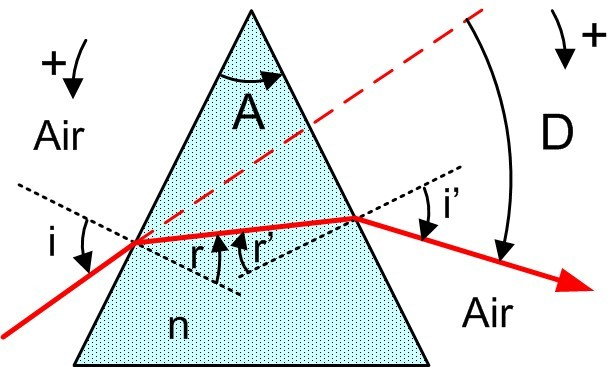
\includegraphics[scale=1.0]{./prisme.jpg}
    \caption{Représentation d'un prisme d'angle \(A\)}\label{fig:prisme}%
\end{figure}

\subsection{Les formules du prisme}
\label{chap6-subsec:formulesprisme}

Les deux premières formules traduisent la deuxième loi de Descartes pour la réfraction : \(\sin(i) = n\sin(r)\) et \(\sin(i') = n\sin(r')\). Les deux autres sont géométriques : \(r+r'=A\) et \(D=i+i'-A\). \(D\) est la déviation, c'est l'angle entre le rayon incident et le rayon émergeant. \emph{Un rayon lumineux est toujours dévié vers la base du prisme, \(D \geq 0\)}.

\subsection{Étude de la déviation en fonction de l'angle d'incidence}
\label{chap6-subsec:etudedeviation}
\paragraph{Existence d'un minimum de déviation}

Pour une lumière monochromatique donnée et un prisme donnée, \(n\) et \(A\) sont constants. Les formules du prisme donnent alors:
\(r = \arcsin{\frac{\sin(i)}{n}}\) et donc \(r'=A - \arcsin{\frac{\sin(i)}{n}}\) et donc aussi \(i' = \arcsin n\sin (A-\arcsin(\sin(i)/n))\), donc finalement~:
\begin{equation}
  D = i + \arcsin{n\sin\left(A-\arcsin{\frac{\sin(i)}{n}}\right)} -A.
\end{equation}
Cette fonction, \(D=f(i)\) est assez compliquée à étudier, mais on peut montrer qu'elle admet un seul extremum, qui est d'ailleurs un minimum. On peut le confirmer par expérience.

\paragraph{Symétrie au minimum de déviation}

La loi du retour inverse de la lumière implique que si \(i\) prend la valeur \(i_1\) et \(i'\) la valeur \(i_2\) pour un sens donné de la lumière, alors, pour le sens inverse, \(i=i_2\) et \(i'=i_1\). La déviation est la même pour les deux sens de la lumière. Donc, à chaque valeur de \(D\), il correspond deux angles d'incidence possibles. Mais au minimum de déviation \(D_m\) il n'en correspond qu'un seul.

Pour \(D=D_m\), on a \(i=i'\) et par conséquent \(r=r'\), \emph{la figure est alors symétrique par rapport au plan bisecteur du dièdre formé par le prisme.} En indiçant par \(m\) les valeurs correspondantes au minimum de déviation, on a~: \(r_m = r'_m = \frac{A}{2}\), \(D_m = 2i_m-A\), d'où \(i_m = \frac{D_m+A}{2}\) ; avec \(\sin(i_m) = n\sin(r_m)\), on obtient~:
\begin{equation}
    n = \frac{\sin\left(\frac{D_m+A}{2}\right)}{\sin\left(\frac{A}{2}\right)}
\end{equation}

\paragraph{Déviation maximale, condition d'émergence}

Un rayon lumineux pou\-rra de toute façon traverser la face d'entrée du prisme quel que soit son angle d'incidence, mais il ne traversera la face de sortie que si son angle d'incidence \(r'\) sur celle-ci est inférieur à \(i_m = \arcsin 1/n\) ce qui correspond à \(i'_0 = \frac{\pi}{2}\) et à \(r_0 = A - \arcsin 1/n\) donc à l'angle d'incidence minimal \(i_0 = \arcsin(n\sin(A-\arcsin 1/n))\). On remarquera que cet angle peut être positif ou négatif suivant la valeur du prisme \(A\). La déviation prendra alors sa valeur maximale, la même que pour \(i=\frac{\pi}{2}\), d'après la loi du retour inverse de la lumière~:
\begin{equation}
    D_m = i_0 +\frac{\pi}{2} - A
\end{equation}

\subsection{Exemple}\label{chap6-subsec:exemple}
Soit un prisme d'angle au sommet \(A = \frac{\pi}{6}\), d'indice \(n=\frac{3}{2}\) pour une lumière monochromatique considérée.

Au minimum de déviation, \(r=r'=r_m=\frac{A}{2}=\frac{\pi}{12}\), et \(i=i'=i_m=\arcsin\left(\frac{3}{2}\sin(\pi/12)\right) = \arcsin\left(\frac{3}{2} \frac{\sqrt{2-\sqrt{3}}}{2}\right)\) soit 22.8 degrés, et \(D_m=2i_m-A\) vaut approximativement 15.7 degrés.
L'angle d'incidence minimal permettant la traversée de la deuxième face du prisme est \(i_0\) tel que \(i'_0=\frac{\pi}{2}\), d'où \(r'_0 = \arcsin(1/n)\) soit approximativement 41.8 degrés et \(r_0=A-r'_0\) soit -11.8 degrés d'où \(i_0=\arcsin(1.5 \sin(r_0))\) soit approximativement -17.9 degrés. La déviation maximale est donc de \(D_0 = i_0 + \frac{\pi}{2}-A\) approximativement 42.1 degrés. Elle est obtenue pour \(i=i_0\) et \(i'=\frac{\pi}{2}\) comme pour \(i=\frac{\pi}{2}\) et \(i'=i_0\).

Pour \(i=0\) on a \(r=0\), \(r'=A=\frac{\pi}{6}\). On a alors \(i'=\arcsin(\frac{3}{2}\sin(\pi/6))\) soit approximativement 48.6 degrés et une déviation \(D=i'-A\) soit approximativement 18.6 degrés. La même déviation est obtenue pour \(i\) valant 48.6 degrés et \(i'=0\).
Le tracé complet de \(D=f(i)\) est réalisé ci-dessous sur la figure~\ref{fig:chap6-deviation}, directement avec l'expression de cette fonction.
\begin{figure}
    \centering
    \includegraphics[width=\textwidth]{Deviation.png}
    \caption{Déviation en fonction de l'incidence}
    \label{fig:chap6-deviation}
\end{figure}
\subsection{Étude de la déviation, dispersion polychromatique}

On retiendra d'abord que \emph{l'indice d'un milieu transparent est une fonction croissante de la fréquence de la lumière, donc décroissante en fonction de la longueur d'onde dans le vide}.

En effet, pour les radiations lumineuse (aussi dans l'infrarouge et l'ultraviolet), mais pas au delà,\emph{la lumière est d'autant plus freinée que ses photons ont plus d'énergie}, donc si \(E=h \nu\) croît, alors la longueur d'onde dans le vide \(\lambda_0 = h/\nu\) décroît, la vitesse \(v\) décroît et donc l'indice de réfraction par rapport à l'aire \(n=c/v\) croît. À la lumière violette correspond un indice plus élevé que pour la lumière rouge.

Il en résulte qu'un rayon entrant dans un milieu moins réfringent est d'autant plus dévié (rapproché de la normale) que sa longueur d'onde dans le vide est basse. De même, un rayon entrant dans u milieu moins réfringent est d'autant plus dévié (écarté de la normale) que lorsque sa longueur d'onde dans le vide est plus basse.

Pour un rayon lumineux traversant le prisme, les deux déviations \(i-r\) et \(i'-r'\) (dont la somme est \(D\)) se font dans le même sens, vers la base du prisme ; donc, pour un angle d'incidence fixé, \emph{un rayon lumineux est d'autant plus dévié par un prisme que sa longueur d'onde dans le vide est plus basse.}
\emph{Un prisme permet donc de disperser une lumière polychromatique plus efficacement, grâce aux deux réfractions, qu'un réfraction unique}.

\section{Exercices}

\begin{exercice}[Conditions d'émergences pour le prisme]
    Soit un prisme d'indice \(n\), plongé dans l'air d'indice 1, d'angle \(A\).
    Soit \(S\) la source lumineuse ponctuelle et \(SI\) un rayon incident contenu dans un plan de section principale, \(I\) étant le point d'incidence. Le rayon réfracté par la première face frappe la seconde face du prisme en \(I'\). Le rayon réfracté par la seconde face est \(I'R\), lorsqu'il existe.

    On utilisera les notations et les conventions de signes habituelles pour les angles \(i\), \(i'\), \(r\) et \(r'\) et \(D\).
    \begin{enumerate}
\item Montrer que, lorsqu'il existe, le rayon \(I'R\) est dans le plan de section principale de \(SI\).
\item Établir les quatre formules du prisme.
\item Montrer que pour que le rayon \(I'R\) existe, il est nécessaire que les deux conditions suivantes soient satisfaites : \(A \leq 2 \arctan(1/n)\) et \(i_0 \leq i \leq \pi/2\) avec \(\sin i_0 = n \sin\left(A-\arcsin(1/n)\right)\).
    \end{enumerate}
\end{exercice}

\begin{exercice}[Étude du minimum de déviation]
    Les notations sont celles de l'exercice précédent.
    \begin{enumerate}
        \item
        \begin{enumerate}
            \item Montrer que la déviation \(D\) passe par un minimum \(D_m\) lorsque \(ii=i'=i_m\).
            \item Exprimer l'indice \(n\) du prisme en fonction de \(A\) et \(D_m\).
            \item Tracer l'allure de la courbe de \(D=f(i)\). On précisera les tangentes aux deux extrémités \(i=i_0\) et \(i=\pi/2\), ainsi que la valeur de la déviation \(D_0\) correspondante.
            \item Quel est d'après vous l'intérêt d'utiliser le prisme au minimum de déviation ?
        \end{enumerate}
        \item Dans un spectroscope à prisme, le prisme est éclairé en lumière parallèle (donc sous une incidence \(i\) fixée), est monochromatique, de longueur d'onde dans le vide \(\lambda\), variable. Exprimer \(\derived{D}{\lambda}\), en fonction de \(\derived{n}{\lambda}\) (dispersion du verre du prisme), \(A\), \(r\) et \(i'\).
        \item On se place au minimum de déviation pour une longueur d'onde \(\lambda\) donnée. Le faisceau incident est obtenu grâce à une fente éclairée par la source, parallèle à l'arête du prisme et une lentille convergente \(L_1\), de distance focale \(f'\), placée entre la fente et le prisme. Le spectre obtenu est recueilli sur une plaque photographique dans le plan focal d'une lentille convergente \(L_2\) de même distance focale \(f'\) que \(L_1\). La base de la partie éclairée du prisme a une largeur \(b\), celui-ci est éclairé jusqu'à son arête. Le faisceau émergent a une largeur égale à \(a\) dans les plans de section principale du prisme. Exprimer \(\derived{D}{\lambda}\) en fonction de \(a\), \(b\) et \(\derived{n}{\lambda}\).
    \end{enumerate}
\end{exercice}

\begin{exercice}[Fibre optique à saut d'indice]
    Soit une fibre optique \(F\) constituée d'un cœur cylindrique de rayon \(a\) et d'indice \(n_1\), entouré d'une gaine d'indice \(n_2 \leq n_1\) et de rayon extérieur \(b\). Les faces d'entrées et de sortie sont perpendiculaires au cylindre d'axe \((Oz)\) formé par la fibre. L'ensemble, en particulier la face d'entrée, est en contact avec un milieu d'indice \(n_0\) et pour les applications numériques, on considérera que ce milieu est de l'air \(n_0=1\).
    \begin{enumerate}
        \item "Zigzag plan". Un rayon lumineux \(SI\) arrive en un point \(I\) sur la face d'entrée de la fibre. À quelles conditions d'incidence ce rayon a-t-il, dans la fibre, un trajet plan ?

        On considère un rayon \((SI)\) incident sur le cœur et contenu dans le plan \(Oxz\). On appelle \(i\) l'angle d'incidence et \(\theta\) l'angle de la réfraction sur la face d'entrée de la fibre.
        \item Déterminer en fonction de \(n_0\), \(n_1\) et \(n_2\) la condition que doit satisfaire \(i\) pour que le rayon réfracté ait une propagation guidée dans le cœur. la valeur maximale de \(i\) est alors désignée par \(i_a\), l'angle d'acceptance de la fibre.
        \item On appelle ouverture numérique \(ON\) du guide la quantité \(ON=n_0 \sin i_a\). Exprimer l'ouverture numérique en fonction de \(n_1\) et \(n_2\).
        \item Calculer \(i_a\) et \(ON\) pour une fibre d'indice \(n_1=1.456\) (silice) et \(n_2=1.410\) (silicone). Quelles seraient les valeurs de ces grandeurs pour un guide à base d'arséniure de gallium pour lequel \(n_1=3.9\) et \(n_2=3\) ? Commenter

        L'atténuation de la lumière dans les fibres optiques est due à l'absorption et à la diffusion par le matériau constitutif du cœur et par ses impuretés (les ions fers 2, les ions cuivres 2, les ions hydroxyde, \ldots). Elle se mesure en décibels par kilomètre : \(A=\frac{\SI{10}{km}}{l} \log(\Phi_1/\Phi_2)\), où \(\Phi_1\) et \(\Phi_2\) désignent les flux lumineux (puissance lumineuse) dans les plans de front successifs 1 et 2 distants de \(l\).

        \item On parvient couramment à réaliser des fibres dans lesquelles le flux, après un parcours de 50 kilomètres, représente 10 pourcents du flux incident. Calculer l'atténuation de telles fibres. Applications : Endoscope à fibres, fibroscope. Le but d'un endoscope est de permettre à un observateur de "voir" dans des endroits inaccessibles, d'intérêts divers (médical, militaire, industriel, \ldots). L'endoscope à fibres est constitué de deux faisceaux de fibres : l'un éclaire le site, l'autre assure le retour vers l'extérieur de la lumière émise par la cible éclairée. Le nombre de fibres constituant chaque faisceau est de l'ordre de 10 mille à 1 million.

        \item Si l'on imagine la cible divisée en 100 mille petits carrés à peu près, chaque fibre au voisinage de la cible recueillant la lumière de l'un d'eux, quel est le problème posé à l'autre extrémité par la reconstitution de l'image ? Quel est le problème technologique majeur posé alors par la fabrication d'un faisceau de fibres ?
    \end{enumerate}


\end{exercice}

\chapter{Formation des images, miroir plan, miroir sphérique}
\label{chap:formationdesimages}
\minitoc
\minilof
\minilot
\section{Point objet, point image, stigmatisme}
\label{chap7-sec:pointobjet}

\subsection{Stigmatisme d'un système optique pour un point}
\label{chap7-subsec:stigmatisme}

Soit un système optique utilisant l'optique géométrique (réflexions et réfractions), frappé par un faisceau lumineux monochromatique, dont les rayons (rayons incidents) sont portés par des droites concourantes. Le point de concours de ces droites est un point objet. Celui-ci peut se trouver sur le trajet des rayons lumineux ou sur leurs prolongements.

Si les droites supports des rayons émergeant du système optique sont concourantes, on dit que le système est stigmatique pour le point objet considéré. Le point de concours des droites supports des rayons émergents est le point image correspondant au point objet considéré.

\emph{Un système optique stigmatique pour un point objet donné, (intersection des supports des rayons incidents), donne de ce point objet un point image, (intersection des supports des rayons émergents).}

Un point objet et le point image correspondant sont dits ``conjugués'' par rapport au système optique.

\subsection{Réalité, virtualité d'un point objet ou d'un point image}
\label{chap7-subsec:realitevirtualite}

Si un système optique est stigmatique pour un point objet donné, le point objet est réel s'il est avant l'entrée dans le système et virtuel s'il se trouve après. Le point image est réel s'il se trouve après la sortie du système et virtuel s'il se trouve avant. On retiendra les définitions suivantes qui sont équivalentes.

\emph{Un point objet est réel si les rayons incidents divergent et virtuel s'ils convergent, à l'entrée dans le système optique. Un point image est réel si les rayons émergents convergent et virtuel s'ils divergent à la sortie du système optique.}

\subsection{Objets et images étendus}
\label{chap7-subsec:objetsimagesetendues}

Un ensemble de points objets constitue un objet étendu. Si le système optique considéré est stigmatique pour tous ces points, l'ensemble des points image correspondants constitue une image étendue.


\section{Images données par un miroir plan}
\label{chap7-sec:imagemiroirplan}

Les lois de Descartes pour la réflexion impliquent qu'à tout rayon incident dont le support passe par un point objet donné correspond un rayon émergent dont le support passe par le symétrique du point objet par rapport au plan du miroir. Celui-ci est donc le point image correspondant.

\emph{Un miroir plan est stigmatique pour tout point objet. L'image d'un objet donnée par un miroir plan est symétrique de l'objet par rapport au plan du miroir.}

Si l'objet est une source de lumière, source primaire, produisant elle-même de la lumière, ou source secondaire, éclairée et diffusant la lumière qu'elle reçoit, c'est-à-dire la réfléchissant dans toutes les directions du fait de la structure plus ou moins granulaire de sa surface, 1'objet est réel et l'image est virtuelle.

Si l'objet est l'image que formerait un système optique (projecteur) sur un écran si la lumière n'était pas déviée avant celui-ci par le miroir, il s'agit pour le miroir d'un objet virtuel et son image est réelle, on peut l'observer sur un écran diffusant convenablement placé. Si l'objet est plan son image l'est aussi).

\section{Miroir sphérique}
\label{chap7-sec:miroirspherique}

\subsection{Définitions}
\label{chap7-subsec:definitions}

Un miroir sphérique est constitué par une calotte sphérique réfléchissante. Le centre $C$ de la sphère dans laquelle a été découpé le miroir est le centre du miroir. Le rayon $r$ de cette sphère est le rayon du miroir. L'axe de la calotte sphérique est l'axe principal ou axe optique du miroir. Son intersection $S$ avec le miroir est le sommet du miroir. Le demi angle au sommet $a$ du cône de sommet $C$ qui délimite le miroir est l'angle d'ouverture du miroir. Les droites passant par $C$ sont les axes secondaires du miroir.
Si le centre $C$ est dans le milieu de propagation de 1a lumière, le miroir est concave. Il est convexe dans le cas contraire.

\subsection{Condition de stigmatisme rigoureux}
\label{chap7-subsec:conditiondestigmatisme}

On prendra l'exemple d'un point objet réel $A$ sur l'axe principal d'un miroir sphérique concave.
Un rayon lumineux issu de $A$, suivant l'axe principal est réfléchi en $S$ avec un angle d'incidence nul.
 L'angle de réflexion est donc aussi nul et le rayon réfléchi suit l'axe principal en sens inverse. Donc, si $A$ a un conjugué, celui-ci se trouve aussi sur l'axe principal.
Soit un autre rayon issu de $A$, frappant le miroir au point d'incidence $I$, avec l'angle d'incidence $i$. On notera $\omega$ l'angle de la normale au point d'incidence avec l'axe principal.
D'après les lois de Descartes, le rayon réfléchi coupe l'axe principal, en un point $A$, puisqu'il est dans le plan de $A$, $C$ et $I$ et l'angle de réflexion est égal à $i$.
$A'$ est le conjugué de $A$ si et seulement si la position de $A'$ est indépendante de l'angle $\omega$, (ou de $I$, ou de $i$).

On a~:
\begin{equation}
  \tan(\omega-i) = \frac{\tan \omega -\tan i}{1+ \tan\omega \tan i} = \frac{IH}{\overline{CH} - \overline{CA}}.
\end{equation}
Avec $H$ le projeté de $I$ sur l'axe du miroir, $IH = \overline{CS} \sin \omega$ et $\overline{CH} = \overline{CS} \cos \omega$. En posant $a = \frac{\overline{CA}}{\overline{CS} \cos \omega}$ on obtient
\begin{equation}
  \tan(\omega-i) = \frac{\tan \omega -\tan i}{1+ \tan\omega \tan i} =\frac{\tan \omega}{1-a}
\end{equation}
d'où
\begin{equation}
  \tan i = - \frac{a \tan \omega}{1-a+\tan^2 \omega}.
\end{equation}

De la même manière, en posant $a' = \frac{\overline{CA'}}{\overline{CS} \cos \omega}$ on obtient
\begin{equation}
  \tan(\omega+i) = \frac{\tan \omega +\tan i}{1+ \tan\omega \tan i} =\frac{\tan \omega}{1-a'},
\end{equation}
d'où
\begin{equation}
  \tan i = \frac{a' \tan \omega}{1-a+\tan^2 \omega}.
\end{equation}

Avec les deux expressions de $\tan i$, on obtient
\begin{equation}
  -a +aa' -a\tan^2\omega = a'-a'a+a'\tan^2\omega,
\end{equation}
d'où
\begin{equation}
  2aa' = \frac{a+a'}{\cos^2\omega}.
\end{equation}
En remplaçant $a$ et $a'$ on obtient
\begin{equation}
  2 \frac{\overline{CA}\overline{CA'}}{\overline{CS}^2\cos^2\omega} = \frac{\overline{CA} + \overline{CA'}}{\overline{CS} \cos^3\omega},
\end{equation}
d'où
\begin{equation}
  \label{eq:stigrigoureux}
  2 \overline{CA} \overline{CA'} \cos\omega = \overline{CS}(\overline{CA}+ \overline{CA'}).
\end{equation}
Ainsi
\begin{equation}
  \overline{CA'} = \frac{\overline{CA} \overline{CS}}{2 \overline{CA} \cos \omega - \overline{CS}},
\end{equation}
et en dérivant
\begin{equation}
  \derived{\overline{CA'}}{\omega} = 2 \frac{\overline{CA}^2 \overline{CS} \sin\omega}{(2 \overline{CA} \cos \omega - \overline{CS})^2}.
\end{equation}

Pour qu'il y ait stigmatisme rigoureux, il faut que pour tout $\omega$, $\derived{\overline{CA'}}{\omega} = 0$. En dehors du cas où $\overline{CS}=0$ qui n'a aucun intérêt et $\overline{CS}=\infty$ qui est la cas du miroir plan, la seule possibilité est que $\overline{CA}=0$. Alors~:
\emph{Un miroir sphérique n'est exactement stigmatique que  pour un seul point objet, son centre. Le centre d'un miroir sphérique est son propre conjugué.}

\subsection{Stigmatisme approché}
\label{chap7-subsec:stigmatismeapproche}

Si tous les rayons issus de A sont paraxiaux, c'est-à-dire voisins de l'axe principal, on peut faire l'approximation $\cos \omega = 1$. L'équation \ref{eq:stigrigoureux} se ré-écrit alors en
\begin{equation}
  2 \overline{CA} \overline{CA'} = \overline{CS}(\overline{CA}+ \overline{CA'}),
\end{equation}
alors
\begin{equation}
  \frac{1}{\overline{CA}} + \frac{1}{\overline{CA'}} = \frac{2}{\overline{CS}}.
\end{equation}

On remarque que si $A'$ est le conjugué de $A$, alors $A$ est le conjugué de $A'$ (c'est une conséquence de la loi du retour inverse). Lorsque tous les rayons sont paraxiaux, on dit que le miroir sphérique est utilisé dans les \emph{conditions de Gauss}.

\subsection{Aplanétisme, notion de plans conjugués, conditions de Gauss, grandissement transversal}
\label{chap7-subsec:aplanetisme}

Soit un point $A$ de l'axe principal et $A'$ son conjugué dans les conditions de Gauss. $AB$ est un petit objet dans un plan frontal, c'est-à-dire perpendiculaire à l'axe principal. $B$ est sur un axe secondaire; si les rayons issus de $B$ sont voisins de l'axe principal, ils le sont aussi de l'axe secondaire $CB$ si $AB$ est suffisamment petit. $B$ a donc un conjugué $B'$ tel que $\frac{1}{\overline{CB}}+\frac{1}{\overline{CB'}} = \frac{2}{\overline{CS'}} = \frac{2}{\overline{CS}}$. Mais AB étant petit, $\overline{CA}=\overline{CB}$, $\overline{CA'} \approx \overline{CB'}$ et l'image $A'B'$ est à peu près perpendiculaire à l'axe principal, c'est-à-dire \emph{contenue dans un plan frontal} dont on dira qu'il est \emph{conjugué du plan frontal de l'objet}.
Lorsqu'il en est ainsi pour un système centré, c'est-à-dire présentant une symétrie de révolution autour d'un axe appelé axe optique du système, on dit que celui-ci est \emph{aplanétique}.
On peut remarquer d'autre part que pour que les conditions de Gauss soient respectées à la fois pour $A$ et pour $B$, il faut et il suffit que l'angle d'incidence $i$ d'un rayon issu de $B$ et passant par $S$ soit très petit et que l'angle $\alpha$ d'ouverture utile du miroir le soit aussi. (On peut limiter l'ouverture utile du miroir avec un diaphragme).

\emph{Conditions de Gauss : objet petit devant le rayon du miroir et ouverture utile du miroir très faible (alors tous les rayons issus de l'objet et frappant le miroir sont paraxiaux). Le grandissement transversal est par définition le rapport des dimensions algébriques de l'image et de l'objet situés dans des plans frontaux conjugués} $\gamma = \frac{\overline{A'B'}}{\overline{AB}}$.

Pour le miroir sphérique on obtient immédiatement $\gamma = \frac{\overline{CA'}}{\overline{CA}}$.

\subsection{Formules du miroir sphérique avec origine au centre et avec origine au sommet}
\label{chap7-subsec:formulemiroirspherique}

Les formules déjà démontrées sont les formules de Descartes du miroir sphérique avec origine au centre : formule de conjugaison $\frac{1}{\overline{CA}} + \frac{1}{\overline{CA'}} = \frac{2}{\overline{CS}}$, formule du grandissement transversal $\gamma = \frac{\overline{CA'}}{\overline{CA}}$.
Le sens positif étant celui de la lumière incidente dans la direction de l'axe principal et celui de l'objet $AB$ dans la direction perpendiculaire. Ces formules ne sont valables que si l'image existe, c'est-à-dire si les conditions de Gauss sont respectées. On supposera dorénavant qu'il en est ainsi, même si pour des raisons pratiques les figures sont dilatées dans la direction perpendiculaire à l'axe principal.
Elles conviennent que le miroir soit concave ou convexe.

En plaçant maintenant l'origine au sommet, on obtient $ \frac{1}{\overline{SA} - \overline{SC}} + \frac{1}{\overline{SA'} - \overline{SC}} = -\frac{2}{\overline{SC}}$, en réduisant au même dénominateur et en multipliant par ce dénominateur $\overline{SC}(\overline{SA}+\overline{SA'}-2\overline{SC})=-2(\overline{SA}-\overline{SC})(\overline{SA'}-\overline{SC})$, après simplification il reste : $0= -2\overline{SA}(\overline{SA'}+\overline{SA}\overline{SC} +\overline{SA'}\overline{SC})$. En divisant par $\overline{SA}\overline{SA'}\overline{SC}$, on obtient finalement : $\frac{1}{\overline{SA}} + \frac{1}{\overline{SA'}} = \frac{2}{\overline{SC}}$.

Formules de Descartes du miroir sphérique avec origine au sommet : formule de conjugaison $\frac{1}{\overline{SA}} + \frac{1}{\overline{SA'}} = \frac{2}{\overline{SC}}$, formule du grandissement transversal $\gamma = -\frac{\overline{SA'}}{\overline{SA}}$.

\subsection{Foyer principal, plan focal, distance focale}
\label{chap7-subsec:foyerprincipal}

Pour un système optique centré, en général on nomme \emph{foyer principal image le point image conjugué du point objet situé à l'infini sur l'axe principal et foyer principal objet le point objet conjugué du point image situé à l'infini sur l'axe principal.}

\emph{Les foyers principaux image et objet du miroir sphérique sont confondus en un point $F$ nommé foyer principal du miroir, situé sur l'axe principal, à égale distance du centre et du sommet.}

On nomme distance focale 1a distance algébrique $f = \overline{SF}$ (avec pour sens positif celui de la lumière incidente). Distance focale : $f = \overline{SF} = \overline{FC} = \frac{\overline{SC}}{2}$, pour un miroir concave $f < 0$ , pour un miroir convexe $f > 0$. Le plan focal est le plan frontal qui contient le foyer principal. Son plan frontal conjugué est donc à l'infini.

De la définition du foyer principal, il résulte que : \emph{tout rayon incident parallèle à l'axe principal émerge en passant par le foyer principal. Tout rayon incident passant par le foyer principal émerge parallèlement à l'axe principal.}

\subsection{Foyers secondaires}
\label{chap7-subsec:foyerssecondaires}

Pour un axe secondaire, peu incliné sur l'axe principal, on a les mêmes propriétés : l'intersection d'un axe secondaire avec le plan focal est le foyer secondaire correspondant (noté $\Phi$), c'est le conjugué du point à l'infini de cet axe secondaire. Tout rayon incident (paraxial) parallèle à un axe secondaire donné émerge en passant par le foyer secondaire correspondant. Tout rayon incident (paraxial) passant par un foyer secondaire donné émerge parallèlement à l'axe secondaire correspondant.

\subsection{Représentation du miroir sphérique utilisé dans les conditions de Gauss, construction des images}
\label{chap7-subsec:miroirspheriqueconditionsdeGauss}

Pour qu'un miroir sphérique soit utilisé dans les conditions de Gauss, il est nécessaire que les rayons lumineux soient paraxiaux, donc qu'ils frappent le miroir prés de son sommet. La partie utile du miroir est donc pratiquement un plan de front d'où sa représentation (toujours fortement dilatée dans la direction perpendiculaire à l'axe principal, pour faciliter les constructions graphiques).

Les propriétés des foyers secondaires permettent de construire le rayon émergent correspondant à un rayon incident paraxial donné.

Pour construire l'image d'un petit objet $AB$ situé dans un plan frontal, $A$ étant sur l'axe principal, il suffit d'utiliser les propriétés du foyer principal pour obtenir l'image $B'$ de $B$. (On peut aussi utiliser le fait qu'un rayon passant par $C$ se réfléchi en revenant sur lui-même). L'image $A'$ de $A$ sera dans le même plan frontal que $B'$.

Exemple avec un miroir concave, un objet réel, une image réelle, renversée, plus petite que l'objet. Exemple avec un miroir convexe, un objet réel, une image virtuelle, droite, plus petite que l'objet. 

\subsection{Formules de Newton (origine au foyer)}
\label{chap7-subsec:formulesdeNewton}

Les homothéties dans les figures ci-dessus permettent  d'écrire (toujours avec $f =  \overline{SF}$) :
\begin{align}
  \gamma &= \frac{\overline{A'B'}}{\overline{AB}} = \frac{\overline{A'B'}}{\overline{SI}} = \frac{\overline{FA'}}{\overline{FS}} = - \frac{\overline{FA'}}{f} \\
\gamma &= \frac{\overline{A'B'}}{\overline{AB}} = \frac{\overline{SI'}}{\overline{AB}} = \frac{\overline{FS}}{\overline{FA}} = - \frac{f}{\overline{FA}}.
\end{align}
D'où $f^2 = \overline{FA}\overline{FA'}$. 

Formule de Newton du grandissement : $\gamma = - \frac{\overline{FA'}}{f} = - \frac{f}{\overline{FA}}$.
Formule de conjugaison de Newton : $f^2 = \overline{FA}\overline{FA'}$.

\subsection{Image d'un objet à l'infini}
\label{chap7-subsec:imageobjetinfini}

On peut utiliser directement la deuxième loi de Descartes ou les propriétés des foyers secondaires. Par exemple, pour un objet réel à l'infini, avec un miroir concave : On constate que l'image est réelle et renversée. Le grandissement est bien sûr nul. L'image est vue de $S$ sous le même angle apparent que l'objet : $\alpha'=\alpha$(angle petit dans les conditions de Gauss). On a donc $A'B' = \alpha |f| \tan(\alpha)$  soit $\overline{A'B'} = \alpha f$.

\section{Exercices}
\label{chap7-sec:exercices}

\begin{exercice}[Association de miroirs]
  On réalise un système optique centré constitué par l'association du miroir concave $M_1$, de centre $C_1$ de sommet $S_1$, et du miroir $M_2$, de centre $C_2$, de sommet $S_2$, de même axe optique. Ils sont disposés tels que : 
$C_1$ -- $C_2$ -- $S_2$ -- $S_1$.

Le miroir $M_1$ est percé d'un petit trou permettant à la lumière de le traverser près de son sommet, mais qui ne modifie pas ses propriétés.
Les distances focales $f_1$ et $f_2$ des deux miroirs sont telles que $|f_1| = \SI{3.0}{m}$ et $|f_2| = \SI{2.0}{m}$. On note $d = \overline{S_1 S_2}$.
\begin{enumerate}
\item Déterminer $d$ pour que tout rayon incident, parallèle à l'axe optique et réfléchi par les deux miroirs, passe par $S_1$.
\item Vérifier le calcul par une construction graphique à l'échelle $0,02$ pour les segments parallèles à l'axe optique. (L'échelle dans la direction perpendiculaire à l'axe optique sera prise bien plus grande).
\end{enumerate}
\end{exercice}
%
\begin{exercice}[Cavité confocale]
  Une cavité confocale est constituée de deux miroirs identiques concaves $M_1$ et $M_2$ face à face, de même rayon $R$, de même axe optique $\Delta$ et dont les foyers sont confondus. On place un objet $AB$ à l'intérieur de la cavité perpendiculairement à $\Delta$.
%
  \begin{enumerate}
  \item Construire géométriquement les quatre images successives obtenues, la première réflexion ayant lieu sur $M_2$. Le résultat dépend-il de la position de l'objet $AB$?
  \item On considère un rayon lumineux, incliné d'un angle $\alpha_1$ sur l'axe optique, émis d'un point $B$ et dont le support passe par le point $I_1$ de $M_1$ distant de $y_0$ de l'axe optique.

    Exprimer en fonction de $\alpha_1$, $y_0$ et $R$ dans les conditions de Gauss, les angles $\alpha_2$, $\alpha_3$, $\alpha_4$ que font les rayons réfléchis avec $\Delta$ à l'issue respectivement de la 1\iere, 2\ieme puis 3\ieme réflexion.
  \item Conclure quant à la localisation du rayon à l'intérieur de la cavité optique.
  \end{enumerate}
\end{exercice}
%
\begin{exercice}[Télescope Hipparcos (D'après écrit Mines sup 2000  filière PCSI option PC)]
  On propose de modéliser le télescope d'Hipparcos par un miroir concave $M_C$ de rayon $R = \SI{2800}{mm}$ avec un miroir plan de renvoi. On note $S$ le sommet du miroir concave. La lumière subit deux réflexions et passe par un orifice dans le miroir concave pour atteindre le détecteur. Celui-ci est constitué d'une grille et de cellules CCD permettant de repérer la position de l'image. La grille comporte $N = 2688$ fentes équidistantes de $L = \SI{8,2}{\micro\meter}$.

On considère une étoile visée dans la direction $Sx$. L'axe $Sx$ est orienté vers l'étoile.
\begin{enumerate}
\item Déterminer l'abscisse $x$ de l'image $E_1$, de l'étoile $E$ donnée par le miroir $M_C$.
\item On note $a$ la distance séparant le miroir plan et le sommet du miroir concave. Déterminer une condition sur $a$ pour que l'image finale $E_2$ se forme sur le détecteur placé à l'arrière du miroir concave.
\item Déterminer la largeur angulaire $\alpha_C$ du champ observé. Calculer $\alpha_C$ en degré.
\item En réalité, Hipparcos réalise une mesure de position relative des étoiles. Le télescope vise deux directions symétriques par rapport à $Sx$ présentant un angle $\alpha = 58 \degrees$. C'est un système de deux miroirs plans $M_1$, $M_2$ qui permet d'obtenir les images des deux étoiles sur le détecteur. Le télescope tourne autour d'un axe de direction fixe $S_z$. 
Déterminer l'angle $\alpha_0$ des miroirs $M_1$ et $M_2$ avec l'axe $Sx$ du télescope.
\item Déterminer le déplacement angulaire $\theta_1$, d'un rayon lumineux réfléchi par le miroir $M_1$ lorsque le satellite tourne d'un angle $\theta$. Préciser le sens de déplacement des rayons réfléchis par $M_1$ et $M_2$.
\end{enumerate}
\end{exercice}

%%% Local Variables: 
%%% mode: latex
%%% TeX-master: "physique"
%%% End: 

\chapter{Lentilles sphériques minces}
\label{chap:lentillesspheriques}
\minitoc
\minilof
\minilot

\section{Différents types de lentilles sphériques}
\label{chap8-sec:differentstypes}

Une lentille sphérique est forme par un milieu transparent, homogène et optiquement isotrope, limité par deux calottes sphériques. Placée dans l'air, la lentille forme donc \emph{deux dioptres sphériques} traversés successivement par la lumière, c'est-à-dire deux surfaces réfringentes correspondant au passage de la lumière de l'air au milieu qui constitue la lentille, et au passage de ce milieu à l'air.
\emph{L'axe principal d'une lentille est 1a droite qui passe par les centres de courbure des deux faces.}

Les deux réfractions subies par un rayon lumineux tendent à rabattre un rayon lumineux vers la base du prisme constitué par les plans tangents aux points d'incidence. On en déduit ainsi le caractère convergent ou divergent des différents types de lentilles, suivant leur action sur un faisceau lumineux parallèle à l'axe principal.

\section{Lentilles sphériques minces, leurs représentations}
\label{chap8-sec:lentillesspheriquesminces}

\emph{Une lentille sphérique mince est une lentille sphérique dont l'épaisseur, mesurée sur l'axe principal, est petite devant les rayons de courbure de ses deux faces.}
La lentille mince est donc assimilée grossièrement à un plan, le plan de la lentille. L'intersection du plan de la lentille avec son axe principal est le centre optique de la lentille. Tout plan perpendiculaire à l'axe principal est un plan frontal. 

Toute droite passant par le centre optique de la lentille est un axe secondaire de la lentille. Les lentilles minces sont représentées ainsi :
%% Mettre une figure

\section{Conditions de stigmatisme approché pour une lentille mince, conditions de Gauss et aplanétisme}
\label{chap8-sec:conditions}

L'étude du dioptre sphérique n'étant pas au programme, on admettra les résultats suivants sans démonstration. Les conditions de stigmatisme approché sont les mêmes que pour le miroir sphérique; ce sont les conditions de Gauss :
\emph{Une lentille mince est approximativement stigmatique pour des rayons lumineux paraxiaux.}

Utilisée dans ces conditions, la lentille mince est \emph{aplanétique; l'image d'un petit objet contenu dans un plan frontal et voisin de l'axe principal est elle-même contenue dans un plan frontal, conjugué de celui de l'objet.}

\section{Foyers d'une lentille mince}
\label{chap8-sec:foyers}

\subsection{Foyers principaux objet et image}
\label{chap8-subsec:foyersprincipaux}

Les définitions sont les mêmes que pour le miroir sphérique;
\emph{Le foyer principal objet, noté F, est le point de l'axe principal dont l'image est située à l'infini sur l'axe principal. Le foyer principal image, noté F', est le point de l'axe principal image du point objet à l'infini sur l'axe principal.}

Pour une lentille sphérique mince, ces deux points sont distincts, \emph{les deux foyers sont symétriques l'un de l'autre par rapport au centre optique de la lentille}.

\subsection{Plans focaux, distance focale}
\label{chap8-subsec:plansfocaux}

\emph{Les plans frontaux contenant les foyers principaux objet et image sont respectivement nommés plan focal objet et plan focal image de la lentille}. Les distances sont mesurées algébriquement sur l'axe principal avec le sens de propagation de la lumière comme sens positif. \emph{La distance algébrique du centre optique au foyer principal image est la distance focale de la lentille, on la note $f'$}, $f'= \overline{OF'}$. On la nomme encore ``distance focale image'' alors que $f = \overline{OF}= – f'$ est la ``distance focale objet''.

Pour une lentille convergente $f' > 0$ et les deux foyers sont réels. Alors que pour une lentille divergente $f' < 0$ et les deux foyers sont virtuels.

\subsection{Vergence}
\label{chap8-subsec:vergence}

Par définition, la vergence d'une lentille sphérique mince est l'inverse de sa distance focale $C =\frac{1}{f}$. La vergence d'une lentille convergente est positive, celle d'une lentille divergente est négative. Son unité SI est la dioptrie. $1 \delta = \SI{1}{m^{–1}}$.		

On démontre à partir des formules du dioptre (hors programme) que la distance focale dépend des rayons de courbure des faces et de l'indice de la lentille par rapport à l'air par la formule
\begin{equation}
  C = \frac{1}{f'} = (n-1) \left(\frac{1}{R_1} - \frac{1}{R_2}\right),
\end{equation}
avec $R_1 = \overline{OC_1}$ et $R_2 = \overline{OC_2}$ avec $C_1$ et $C_2$ les centres de courbures des deux faces.

\subsection{Foyers secondaires}
\label{chap8-subsec:foyerssecondaires}

L'intersection d'un axe secondaire avec le plan focal objet est un foyer secondaire objet ; c'est le point objet conjugué du point image situé à l'infini sur cet axe secondaire. L'intersection d'un axe secondaire avec 1e plan focal image est un foyer secondaire image ; c'est 1e point image conjugué d'un point objet situé à l'infini sur cet axe secondaire.

\section{Tracé du rayon émergent correspondant à un rayon incident donné}
\label{chap8-sec:trace}

Bien entendu les propriétés énoncées ci-dessous ne sont valables que pour des rayons paraxiaux.

Tout rayon passant par le centre optique ne subit aucune déviation à la traversée de 1a lentille. À tout rayon incident parallèle à l'axe principal (resp. à un axe secondaire) correspond un rayon émergent dont le support passe par le foyer principal image (resp. le foyer secondaire image correspondant).
À tout rayon incident dont le support passe par le foyer principal objet (resp. par un foyer secondaire objet) correspond un rayon émergent parallèle à l'axe principal (resp. à l'axe secondaire correspondant).

\section{Construction de l'image d'un objet frontal donné, dans les conditions de Gauss}
\label{chap8-sec:constructionimagefrontal}

On prendra d'abord l'exemple d'un objet réel situé avant le plan focal objet d'une lentille convergente. On obtient alors une image réelle, donc observable sur un écran diffusant. C'est le cas d'un projecteur de diapositives, d'un appareil photographique, d'un agrandisseur etc.
%%mettre une image
%

Une lentille convergente donne d'un objet réel une image virtuelle, droite, plus grande que l'objet, si l'objet est situé entre le plan focal objet et la lentille. C'est le cas de la loupe ou d'un verre correcteur pour hypermétrope ou presbyte.
%%mettre une image

Une lentille divergente donne d'un objet  réel une image virtuelle droite, plus petite que l'objet. C'est le cas d'un verre correcteur pour myope.
%%mettre une image

On s'exercera en traitant les autres cas, en particulier avec les lentilles divergentes.

\section{Formules des lentilles minces}
\label{chap8-sec:formulesdeslentillesminces}
On note habituellement : $p=\overline{OA}$ et $p'=\overline{OA'}$ on a $f'=\overline{OF'}=\overline{FO}=-f$.

Si $p < 0$ l'objet est réel. Si $p > 0$ l'objet est virtuel. Si $p' < 0$ l'image est virtuelle. Si $p' > 0$ l'image est réelle.

En observant les figures ci-dessus, on constate du fait des homothéties
\begin{equation}
  \gamma = \frac{\overline{A'B'}}{\overline{AB}} = \frac{\overline{A'B'}}{\overline{OI}} = \frac{\overline{OI'}}{\overline{AB}}
\end{equation}
 avec $  \frac{\overline{A'B'}}{\overline{OI}} =  \frac{\overline{F'A'}}{\overline{F'O}}$ et $ \frac{\overline{OI'}}{\overline{AB}} = \frac{\overline{FO}}{\overline{FA}} $ donc $\gamma = \frac{\overline{FO}}{\overline{FA}} = \frac{\overline{F'A'}}{\overline{F'O}}$.

Donc $\frac{f'}{p+f'} = \frac{p'-f'}{f'}$ soit $-f'^2 = -f'^2 + pp' - pf' + p'f'$  et  $pf' - p'f' = pp'$. On obtient la formule de conjugaison en divisant les deux membres par $pp'f'$ .
Formule de conjugaison
\begin{equation}
  \frac{1}{p'} - \frac{1}{p} = \frac{1}{f'} = C.
\end{equation}

D'autre	 part, on obtient directement $\gamma = \frac{\overline{OA'}}{\overline{OA}}$ avec l'homothétie des triangles $OAB$ et $OA'B'$.
Formule du grandissement transversal :
\begin{equation}
  \gamma = \frac{p'}{p}.
\end{equation}
Ce sont les formules de Descartes des lentilles sphériques minces (ou formules avec origine au centre optique). 

Le grandissement $\gamma > 0$ quand $p$ et $p'$ sont de même signe donc quand l'objet est réel et l'image virtuelle ou l'inverse. Le grandissement $\gamma < 0$ quand $p$ et $p'$ sont de signes contraires donc quand l'objet et l'image sont tous deux réels ou tous deux virtuels. Si $\gamma > 0$ l'image est droite, de nature différente de l'objet. Si $\gamma < 0$ l'image est renversée, de même nature que l'objet. Si $|\gamma| > 1$  l'image est plus grande que l'objet, sinon l'image est plus petite que l'objet.

De $\gamma = \frac{\overline{FO}}{\overline{FA}} = \frac{\overline{F'A'}}{\overline{F'O}}$ on tire les formules de Newton ou formules avec origines aux foyers.
Formules du grandissement de Newton : $\gamma = \frac{f'}{\overline{FA}}=-\frac{\overline{F'A'}}{f'}$
Formule de conjugaison de Newton : $\overline{FA}\overline{FA'} = ff' = -f'^2$.

\section{Image d'un objet à l'infini}
\label{chap8-sec:imagealinfini}

On prendra l'exemple d'un objet réel à l'infini. dont une lentille divergente donne une image virtuelle droite.
%% mettre image
%

$B'$ se trouve au foyer secondaire correspondant à l'axe secondaire $BO$. Si la lentille est convergente, l'image est réelle et renversée. L'image et l'objet sont vus de $O$ sous le même angle $\alpha$, toujours petit, si les conditions de Gauss sont respectées, donc $\alpha = tan \alpha = \frac{\overline{A'B'}}{\overline{F'O}} = \frac{\overline{A'B'}}{-f'}$ donc $\overline{A'B'} = -\alpha f'$  (pour $\overline{AB}>0$).

\section{Étude analytique des différents cas}
\label{chap8-sec:etudeanalytique}

%\subsection{Notations utilisées}
%\label{chap8-subsec:notationsutilisees}

De la formule de conjugaison avec origine au centre optique, on tire 
\begin{equation}
  p' = \frac{pf'}{p+f'} \qquad \gamma = \frac{f'}{p+f'}.
\end{equation}

Il est pratique d'utiliser des coordonnées réduites sans dimensions~:
\begin{itemize}
\item Si la lentille est convergente, $f' > 0$, alors on posera $x = \frac{p}{f'}$ et $x' = \frac{p'}{f'}$ donc $x' = \frac{x}{1+x}$ et $\gamma = \frac{1}{1+x}$. Ainsi
  \begin{equation}
    \forall x \ \derived{x'}{x} = \frac{1}{(1+x)^2} > 0 \quad \derived{\gamma}{x} = - \frac{1}{(1+x)^2} < 0.
  \end{equation}
\item Si la lentille est divergente, $f' < 0$, pour que $x$ soit du même signe que $p$ et $x'$ du même signe que $p'$, il est préférable de poser $x = \frac{p}{f}$ et $x' = \frac{p'}{f}$  donc $x' = \frac{x}{1-x}$  et  $\gamma = \frac{1}{1-x}$.
  \begin{equation}
    \forall x \ \derived{x'}{x} = \frac{1}{(1-x)^2} > 0 \quad \derived{\gamma}{x} = - \frac{1}{(1-x)^2} < 0.
  \end{equation}
\end{itemize}

Si l'objet avance dans le sens positif, l'image fait de même, mais avec une discontinuité; elle passe de $+\infty$ à $-\infty$ pour $x = -l$ avec une lentille convergente, et de $-\infty$ à $+\infty$ pour $x = 1$ avec une lentille divergente, c'est-à-dire dans les deux cas, quand l'objet atteint le plan focal objet.
On voit aussi que le grandissement décroît constamment pour une lentille convergente et croit constamment pour une lentille divergente, avec une discontinuité quand l'objet traverse 1e plan focal objet ($x = -1$pour une lentille convergente et $x = 1$ pour une lentille divergente).

\section{Lentilles minces accolées}
\label{chap8-sec:lentillesmincesaccolées}

Si des 	lentilles minces sont accolées, leurs centres optiques co\"incident pratiquement. La première de distance focale $f'_1$, donne de l'objet frontal $AB$ une image $A_1B_1$ qui pour la deuxième lentille est l'objet. La deuxième lentille, de distance focale $f'_2$ donne de $A_1B_1$ une image $A'B'$ qui est aussi l'image de $AB$ donnée par le système des deux lentilles accolées.

En posant $p = \overline{OA}$, $p_1 = \overline{OA_1}$ et $p' = \overline{OA'}$, les formules des lentilles sphériques minces donnent
\begin{equation}
  \frac{1}{p_1} - \frac{1}{p} = \frac{1}{f'_1} \qquad \frac{1}{p'} - \frac{1}{p_1} = \frac{1}{f'_2}
\end{equation}

d'où, par addition membre à membre : $\frac{1}{p'} - \frac{1}{p} = \frac{1}{f'_1} + \frac{1}{f'_2} = C_1 + C_2$. 

Le grandissement de la première lentille est $\gamma_1 = \frac{p_1}{p}$, celui de la deuxième est $\gamma_1 = \frac{p'}{p_1}$, celui du système est donc $\gamma = \gamma_1 \gamma_2 = \frac{p'}{p}$.

\emph{L'ensemble de deux lentilles sphériques minces accolées équivaut à une lentille unique dont la vergence est la somme des vergences des deux lentilles.}

Si les deux lentilles ont des vergences opposées, la vergence du système est nulle. sa distance focale est infinie, c'est-à-dire que ses foyers sont rejetés à l'infini. On a alors un \emph{système afocal}. Dans ce cas, $p' = p$, l'image est identique à l'objet.

Une des possibilités pour mesurer la vergence d'une lentille est de rechercher la lentille de vergence connue qui, accolée à la première, donnera un système afocal. Quelques autres méthodes de \emph{focométrie} (mesure des distances focales) seront étudiées en travaux pratiques.

\section{Exercices}
\label{chap8-sec:exercices}

\begin{exercice}[Montage $4f'$ d'une lentille convergente]
Un objet AB est situé à une distance $2f'$ en avant d'une lentille mince convergente de distance focale image $f'$. Où se trouve l'image $A'B'$ ? Quel est le grandissement ?  
\end{exercice}
%
\begin{exercice}[Lentille biconcave]
Une lentille mince biconcave a des faces sphériques dont les rayons de courbure sont $\SI{0,10}{m}$ et $\SI{0,15}{m}$. Le verre la constituant a un indice valant $1,5$. Où se trouve l'image d'un point objet situé à $\SI{20}{cm}$ en avant de la lentille ?
\end{exercice}
%
\begin{exercice}[Distance entre l'objet et l'image]
On considère une lentille mince convergente de distance focale image $f'$, un point objet $A$ situé sur l'axe et son image $A'$. Étudier les variations de la distance $D = \overline{AA'}$ en fonction de la position de l'objet $A$ par rapport à la lentille.
\end{exercice}
%
\begin{exercice}[Détermination d'une distance focale]
Une lentille mince convergente donne d'un objet une image sur un écran, agrandie deux fois. Lorsqu'on rapproche de $\SI{0,36}{m}$ la lentille de l'écran, la taille de l'image devient la moitié de celle de l'objet. Déterminer la distance focale image de la lentille.
\end{exercice}
%
\begin{exercice}[Mesure de la distance focale d'une lentille par la méthode de Bessel]
Un objet frontal $AB$ et un écran (E) sont fixes et distants de $D$. Entre l'objet et l'écran, on déplace une lentille mince convergente de distance focale image $f'$. Montrer que si $D \geq 4f'$, il existe deux positions de la lentille distantes de $d$ pour lesquelles il y a une image nette de l'objet sur l'écran. Calculer $f'$ en fonction de $D$ et $d$.
\end{exercice}
%
\begin{exercice}[Méthode d'autocollimation]
On accole une lentille mince convergente de distance focale $f'$ et un miroir plan. On éclaire ce dispositif au moyen d'un petit objet lumineux. Lorsque celui-ci est à $\SI{0,1}{m}$ du dispositif, l'image se forme dans le plan de l'objet. Calculer la distance focale de la lentille.
\end{exercice}
%
\begin{exercice}[Position de l'image donnée par un système catadioptrique]
Un système optique est formé d'une lentille mince de distance focale $\SI{0,3}{m}$ et d'un miroir plan disposé à $\SI{0,15}{m}$ de la lentille. Déterminer la position de l'image que ce système donne d'un objet situé à $\SI{0,15}{m}$ en avant de la lentille.
\end{exercice}
%
\begin{exercice}[Construction de l'image donnée par un système catadioptrique]
Construire l'image d'un objet à travers un système optique formé d'une lentille mince et d'un miroir plan disposé dans le plan focal image de la lentille. L'objet est placé en avant de la lentille à une distance comprise entre la distance focale et deux fois la distance focale.
\end{exercice}
%
\begin{exercice}[Points doubles d'un système catadioptrique]
Un système est formé par l'association d'une lentille mince convergente de distance focale $\SI{0,1}{m}$ et d'un miroir plan situé à $\SI{0,2}{m}$ de la lentille. Déterminer le ou les point(s) de l'axe qui est à lui-même, ou qui sont à eux-mêmes, leur propre image. Ces points sont dits points doubles ou points de Bravais.
\end{exercice}
%
\begin{exercice}[Construction de l'image donnée par un système catadioptrique]
Un système optique est formé d'un miroir sphérique concave de distance focale $\SI{0,1}{m}$ et d'une lentille mince convergente de distance focale $\SI{0,2}{m}$. La distance entre la lentille et le miroir est $\SI{0,3}{m}$. Un objet est placé à $\SI{40}{cm}$ de la lentille. Construire son image à travers le système.
\end{exercice}
%
\begin{exercice}[Système catadioptrique afocal]
On associe une lentille divergente et un miroir sphérique concave de façon à ce que le foyer principal image de la lentille soit confondu avec le centre du miroir et que le foyer principal objet de celle-ci soit confondu avec le sommet du miroir. Construire l'image d'un objet dans les conditions de Gauss, déterminer le grandissement transversal.
\end{exercice}
%
\begin{exercice}[Foyers d'un doublet]
Un doublet est formé d'une lentille convergente de distance focale $\SI{15}{cm}$ et d'une lentille convergente de distance focale $\SI{10}{cm}$, les centres optiques des deux lentilles étant distants de $\SI{5}{cm}$. Déterminer les positions des foyers du doublet.
\end{exercice}
%
\begin{exercice}[Doublet afocal]
Une lentille convergente de $\SI{0,3}{m}$ de distance focale et une lentille divergente de $\SI{0,1}{m}$ de distance focale sont distantes de $\SI{0,2}{m}$. Où faut-il placer une source lumineuse pour que ce doublet donne un faisceau de rayons parallèles.
\end{exercice}
%
\begin{exercice}[Étude graphique d'un doublet]
Étudier graphiquement le doublet de symbole (–1; 2; –1).
\end{exercice}
%
\begin{exercice}[Points doubles d'un doublet]
Deux lentilles convergentes (L1) et (L2) de distances focales images $f'_1$, et $f'_2$ forment un système afocal. Soit un objet $AB$ repéré par la distance algébrique $\overline{F_1A}= x1$ et soit son image $A'B'$ à travers le doublet repéré par la distance algébrique  $\overline{F'_2A'}= x_2$. Déterminer les relations de conjugaison du doublet. Application numérique $f'_1  = \SI{20}{cm}$, $f'_2 = \SI{2}{cm}$, déterminer le point de l'axe qui est à lui-même sa propre image.
\end{exercice}
%
\begin{exercice}[Lunette de Galilée]
Une lunette de Galilée est constituée d'une première lentille mince convergente (L1) de distance focale $f'_1 = \SI{0,3}{m}$ (objectif) et d'une seconde lentille mince divergente (L2) de distance focale $f'_2 = -\SI{0,12}{m}$ (oculaire). Ces lentilles sont distantes de $\SI{0,12}{m}$. Au moyen de cette lunette, on observe un objet très éloigné vu sous le diamètre apparent $10'$. Déterminer les caractéristiques de l'image donnée par la lunette.
\end{exercice}
%
\begin{exercice}[Téléobjectif]
Un téléobjectif est formé d'une lentille mince convergente de distance focal image $\SI{5}{cm}$ et d'une lentille mince divergente de distance focale image $-\SI{2}{cm}$ distantes de $\SI{3,5}{cm}$.
À quelle distance de la lentille convergente, l'image d'un objet lointain se forme-t-elle ? Quelle en est la taille si l'objet est vu sous un angle de $5'$ de la première lentille ?
\end{exercice}
%
\begin{exercice}[Téléobjectif]
Un téléobjectif d'appareil photographique est constitué d'une lentille convergente (L1) de distance focale  $f'_1 = \SI{0,06}{m}$ et d'une lentille divergente (L2) de distance focale  $f'_2 = -\SI{0,08}{m}$. Les centres optiques des deux lentilles sont distants de $d = \overline{O_1O_2} = \SI{0,02}{m}$. La pellicule photographique est placée dans le plan focal image du téléobjectif.
\begin{enumerate}
\item Où faut-il disposer cette pellicule ?
\item Construire l'image d'un objet très éloigné.
\item L'objet très éloigné est vu depuis le téléobjectif sous un diamètre apparent de $1'$. Déterminer la grandeur de l'image. 
\end{enumerate}
\end{exercice}
%
\begin{exercice}[Microscope]
Un microscope est constitué d'une lentille mince convergente (L1) de distance focale $f'_1 = \SI{0,002}{m}$ (objectif) et d'une lentille mince convergente (L2) de distance focale $f'_2 = \SI{0,02}{m}$. La distance entre les foyers $F'_1$ et $F_2$ est $d = \SI{0,159}{m}$. Un objet de longueur $\SI{0,01}{mm}$ est placé à $\SI{0,025}{mm}$ du foyer principal objet $F_1$ de (L1) . Déterminer les caractéristiques de l'image donnée par le microscope. Faire une construction géométrique. En déduire les conditions nécessaires pour que le doublet puisse effectivement jouer le rôle de microscope.
\end{exercice}

%%% Local Variables: 
%%% mode: latex
%%% TeX-master: "physique"
%%% End: 
\chapter{Charges électriques, intensité, tension et lois de Kirchhoff}
\minitoc{}
\minilof{}
\minilot{}

\section{Charge électrique}
\label{chap9-sec:chargeelectrique}

\subsection{Électrisation}
\label{chap9-subsec:electrisation}

Elle se fait par frottement, contact ou influence. Elle permet de distinguer isolants et conducteurs : à la surface d'un conducteur les charges sont mobiles (présence d'électrons libres). I1 y a deux types de charges électriques. Une charge négative est due à un excès d'électrons par rapport aux protons; une charge positive est due à un défaut d'électrons. Les atomes concernés par ces excès ou défauts d'électrons sont toujours extrêmement minoritaires.

\subsection{Définition}
\label{chap9-subsec:definition}

Une grandeur physique est dite ``mesurable'' si et seulement si l'on peut définir l'égalité et la somme ou le rapport de deux valeurs de cette grandeur. Soient deux charges \(q\) et \(q'\) ponctuelles, fixes, placées successivement au même point, dans le même environnement électrique (1) et subissant les forces électrostatiques \(\vv{F_1}\) et \(\vv{F'_1}\), puis dans un autre environnement (2), \(\vv{F_2}\) et \(\vv{F'_2}\) etc.

On peut constater par la mesure que \( \frac{F'_1}{F_1} = \frac{F'_2}{F_2} = ...\) Par définition, on pose \(\abs{\frac{q'}{q}} = \frac{F'_1}{F_1}\).
L'unité internationale de la charge électrique est le coulomb, c'est la charge qui traverse toute section d'un circuit parcourue par un courant de \(\SI{1}{A}\) pendant une durée de \(\SI{1}{s}\), donc \(\SI{1}{C} = \SI{1}{A.s}\).

\subsection{Quantification de la charge électrique}
\label{chap9-subsec:quantificationdelachargeelectrique}

Historiquement ceci a été vérifié par l'expérience de Millikan. La charge de tout objet (isolable) est un multiple de la charge élémentaire : \(q = z e\), avec \(z\) un entier relatif. Ceci ne s'applique donc pas aux quarks que l'on ne sait pas séparer les uns des autres. La charge élémentaire vaut \(e = \SI{1,6022e-19}{C}\).
Nombres de charge des particules fondamentales : électron \(z = -1\), proton \(z = 1\), neutron \(z = 0\), positron \(z = 1\), ...,  mais pour les quarks: up (u.) \(z = 2/3\), down (d) \(z = -1/3\).

\subsection{Propriétés des charges électriques}
\label{chap9-subsec:proprietesdeschargeselectriques}

Elles sont invariantes dans un changement de référentiel. La charge électrique est une grandeur extensive conservative. Elle est donc invariable pour un système fermé. Les charges de chaque signe se conservent dans un système fermé en l'absence de toute réaction de création ou d'annihilation de particules.

\section{Densités de charge électrique}
\label{chap9-sec:densitesdechargeelectrique}

\subsection{Densité volumique de charge}
\label{chap9-subsec:densitevolumiquedecharge}

Soit un volume élémentaire \(\D\tau\) autour du point \(M\), portant la charge \(\D q\), la densité volumique de charge en \(M\) est: \(\rho = \derived{q}{\tau}\) (\(\D\tau\) est de l'ordre de \(\SI{1e-24}{m^3}\), \(\D q\) est grand devant la charge élémentaire \(e\)). Son unité internationale est le \(\si{C/m^3}\). Si \(n_i\) est la concentration volumique (nombre par unité de volume en métre cube) des particules de charge \(q_i\), la densité volumique de charge s'écrit encore : \(\rho = \sum_i n_i q_i\).

À l'intérieur d'un conducteur en équilibre électrique, \(\rho = 0\). Les charges éventuelles sont réparties sur la surface du conducteur (voir le cours de deuxième année). Dans un volume \(V\), la charge est \(q=\iiint_V \rho \D V\). Cette écriture signifie simplement que la charge \(q\) est la somme d'un nombre infini de charges infiniment petites. Le signe \(\iiint\) est utilisé ici parce que le volume élémentaire \(\D\tau = \D x \D y \D z\) est le produit de trois différentielles, ce qui implique qu'il faut effectuer trois intégrations, sur les valeurs de \(x\), sur celles de \(y\) et sur celles de \(z\) pour obtenir \(q\).

\subsection{Densité surfacique de charge, densité linéique de charge}
\label{chap9-subsec:densitesurfacique}

Soit un surface élémentaire d'aire \(\D S\) autour du point \(M\), portant la charge \(\D q\), la densité surfacique de charge en \(M\) est : \(\sigma = \derived{q}{S}\). (\(\D S\) de l'ordre de \(\si{1e-16}{m^2}\), \(\D q\) grand devant la charge élémentaire \(e\)). Son unité internationale est le \(\si{C.m^{-2}}\). Sur une surface \(\Sigma\), la charge est \(\iint_\Sigma \sigma \D S\).

Soit une ligne élémentaire de longueur \(\D L\) autour du point \(M\), portant la charge \(\D q\), la densité linéique de charge en \(M\) est : \(\lambda = \derived{q}{L}\). (\(\D L\) de l'ordre de \(\si{1e-8}{m}\), \(\D q\) grand devant la charge élémentaire \(e\)). Son unité internationale est le \(\si{C.m^{-1}}\). Sur une ligne \(\Gamma\), la charge est \(\int_\Gamma \lambda \D L\).

\section{Densités de courant}
\label{chap9-sec:densitedecourant}

\subsection{Densité volumique de courant}
\label{chap9-subsec:densitevolumique}

Soit, pour le \(i\)\ieme type de porteur de charge, au point \(M\) :
\begin{itemize}
\item \(q_i\) : charge de ce type de porteur de charge,
\item \(\rho_i\) : densité volumique de charge mobile (en \(\si{C.m^{-3}}\)),
\item \(\vvv_i\) : vecteur vitesse moyen (en \(\si{m/s}\)),
\item \(n_i\) : concentration volumique (en \(\si{m^{-3}}\)).
\end{itemize}
La densité volumique de courant en \(M\) est \(\vj = \sum_i \rho_i \vvv_i = \sum_i n_i q_i \vvv_i\). Elle s'exprime en \(\si{A.m^{-2}}\).

\subsection{Densité surfacique de courant}
\label{chap9-subsec:Densité surfacique de courant}
Avec des notations semblables, pour des courants circulant sur une surface, la densité surfacique de courant en \(M\) est: \(\vj_s = \sum_i \sigma_i \vvv_i\) .\(\vj_s\) s'exprime en \(\si{A.m^{-1}}\).

\section{Intensité d'un courant électrique}
\label{chap9-sec:intensiteduncourantelectrique}

Soit une surface \(\Sigma\) à travers laquelle circule un courant d'intensité algébrique \(i\). \(\si{A}=\si{C.s^{-1}}\) donc ceci signifie que \(i\) est le nombre d'ampères, c'est-à-dire le nombre de coulombs qui traverse \(\Sigma\) par seconde dans le sens de la flèche qui donne la convention de signe pour \(i\).
%% Inserer figure

\(\vv{\D S}\) représente un vecteur surface élémentaire de norme \(\D S\) autour du point \(M\) (aire élémentaire), normal à la surface \(\Sigma\), orienté dans le sens de la flèche qui définit la convention de signe pour \(i\). Si la densité volumique de charges mobiles, au voisinage de \(M\) est \(\rho\), et si leur vitesse moyenne est \(\vvv\), la densité volumique de courant est \(\vj = \rho \vvv\).
Les charges mobiles contenues dans le cylindre de base , de génératrice \(\vvv \D t\), sont celles qui auront traversé la surface \(\D S\) au bout du temps \(\D t\). Le volume de ce cylindre est \(\D \vv{S} \cdot \vvv\D t\).
La charge qui traverse \(\D S\) pendant le temps \(\D t\) a donc pour expression
\begin{equation}
  \D q = \rho \D \vv{S} \cdot \vvv \D t = \vj \cdot \D S \D t.
\end{equation}

L'intensité du courant traversant la surface \(\D S\) dans le sens défini par la flèche est \(\D i = \derived{q}{t} = \vj \cdot \D \vv{S}\).
Pour obtenir l'intensité totale du courant traversant la surface \(\Sigma\), il faut additionner les intensités élémentaires qui traversent toutes les surfaces élémentaires dont la réunion constitue \(\Sigma\).
L'intensité du courant électrique traversant \(\Sigma\) dans le sens défini par la flèche est donc le ``flux'' du vecteur densité volumique de courant à travers \(\Sigma\)~: \(i = \iint_\Sigma \vj \cdot \D \vv{S}\).

Dans le cas d'un courant surfacique (nappe de courant), pour évaluer le courant  traversant une ligne \(\Gamma\), on fait correspondre à un élément de longueur \(\D L\) de cette ligne un vecteur, normal à la ligne, dans le plan tangent à la surface où circule le courant et orienté dans le sens de la flèche qui définit la convention de signe pour l'intensité. L'élément \(\D L\) est traversé parle courant d'intensité \(\D i = \vj_S \cdot \D \vv{L}\) et l'intensité totale qui traverse la ligne \(\Gamma\) est \(i = \int_\Gamma \vj_S \cdot \D \vv{L}\).

\section{Lignes de courant, tubes de courant}
\label{chap9-sec:lignesdecourant}

En chaque point d'une ligne de courant \(\vj\) est tangent à  cette ligne. Les lignes de courant sont orientées dans le même sens que \(\vj\). Ce sont donc les lignes de champ de la densité volumique de courant. Pour une nappe de courant, ce sont les lignes de champ de la densité surfacique de courant \(\vj_S\).
Les équations d'une ligne de courant sont telles que~: soit un point \(M(x,y,z)\) sur une ligne de courant et un vecteur \(\D M\) joignant \(M\) à un point \(M'\) infiniment voisins de \(M\) sur la même ligne de courant.
\(\D \vv{M} = \D x \ux + \D y \uy + \D z \uz\) est parallèle à \(\vj = j_x \ux + j_y \uy + j_z \uz\) donc \(\frac{\D x}{j_x} = \frac{\D y}{j_y} = \frac{\D z}{j_z}\). L'intégration de ces équations différentielles donne l'équation des lignes de courant.

\emph{Un tube de courant s'appuie sur une courbe fermée et est limité par des lignes de courant.}

Pour une portion de tube de courant limitée par les sections \(\Sigma_1\) et \(\Sigma_2\), avec \(I_1\) courant entrant par \(\Sigma_1\) et \(I_2\) courant sortant par \(\Sigma_2\). Le courant sortant par la paroi \(T\) est nul car en chaque point de \(T\), \(\vj\) est normal à \(\D \vv{S}\) et \(\vj \cdot \D \vv{S} = 0\). Le courant \(i\) sortant de cette portion de tube de courant est donc \(i = I_2 - I_1\).

\section{Régime stationnaire, approximation des régimes quasi-stationnaires (ARQS)}
\label{chap9-sec:ARQS}

\subsection{Définition}
\label{chap9-sec:def}

En régime stationnaire, toutes les grandeurs physiques sont indépendantes du temps (sauf bien entendu les coordonnées des porteurs de charge). Les dérivées partielles par rapport au temps de En régime stationnaire, toutes les grandeurs physiques sont indépendantes du temps (sauf bien entendu les coordonnées des porteurs de charge).
Les dérivées partielles par rapport au temps de \(n_i\), \(\rho_i\), \(\vj\), \(\vvv_i\), T, etc. sont nulles en chaque point. L'approximation des régimes quasi-stationnaires (ARQS) concerne les régimes ``lentement'' variables.

Concrètement, en régime sinusoïdal permanent (courant alternatif sinusoïdal), on peut appliquer cette approximation tant que la fréquence est suffisamment basse pour que la longueur d'onde de la propagation du courant soit grande devant les dimensions du circuit. En notant \(f\) la fréquence et \(v\) la vitesse de propagation du courant (\(v\approx c = \SI{3e8}{m.s^{-1}}\) : vitesse de la lumière dans le vide), cette longueur d'onde est \(\lambda = \frac{c}{f}\).

Pour une fréquence de \(\SI{1}{MHz}\), \(\lambda \approx \SI{300}{m}\), il suffit donc que les dimensions du circuit ne dépassent pas \(\SI{1}{m}\) pour qu'on puisse appliquer l'ARQS.

Pour \(f=\SI{50}{Hz}\) (courants EDF) \(\lambda \approx \SI{6000}{km}\), pour des lignes de transport de plusieurs centaines de kilomètres, l'ARQS ne serait pas très bonne.

\subsection{Tube de courant dans le cadre de l'ARQS}
\label{chap9-subsec:TubedeCourantARQS}

En régime stationnaire, si on note \(q\) la charge électrique contenue dans un volume déterminé, on a \(\derived{q}{t}=0\). Par exemple, pour le tube de courant \(T\), limité par les sections \(\Sigma_1\) et \(\Sigma_2\). Le courant sortant par \(T\) est nul. Le courant sortant est donc \(i = I_2 - I_1\) or \(i=-\derived{q}{t}=0\), donc \(I_1 = I_2\). L'intensité du courant a la même valeur à travers toutes les sections d'une branche du circuit. Pour un tube de courant se partageant en deux branches : On a pour la même raison : \(I = I_1 + I_2\).

En ARQS, ces lois restent valables approximativement, mais les intensités varient (lentement) au cours du temps.

\section{Potentiel électrostatique, tension électrostatique ou différence de potentiel électrostatique}
\label{chap9-sec:potentiel}

\subsection{Potentiel électrostatique}
\label{chap9-subsec:potentiel}

Une répartition de charges (ponctuelles, volumiques, surfaciques ou linéiques) fixe et indépendante du temps crée un champ électrostatique. Le champ électrostatique en un point où une charge \(q\) subit (ou subirait) la force électrostatique \(\vF\)  est \(\vv{E} = \frac{\vF}{q}\), il ne dépend pas de \(q\) mais de la disposition et des valeurs des charges qui créent ce champ.

\emph{Les forces électrostatiques sont conservatives donc elles dérivent d'un potentiel : l'énergie potentielle électrostatique}. Pour un déplacement \(\D \vv{M}\) on a \(\vF \cdot \D \vv{M}=\delta W = -\D E_p\) soit \( q \vv{E} \cdot \D \vv{M}=-\D E_p\) avec \(q\) constante donc \(\D \left(\frac{E_p}{q}\right) = -\vv{E} \cdot \D \vv{M}\).
\(V = \frac{E_p}{q}\) est le potentiel électrostatique au point \(M\), il ne dépend pas de la charge \(q\), ni même de la présence d'une charge électrique en \(M\) puisque sa différentielle est \(\D V = -\vv{E} \cdot \D \vv{M}\) et que \(\vv{E}\) dépend des charges qui le créent et non de celle qui éventuellement le subit.

Son unité internationale est le volt \(\si{V} = \si{J/C} =\si{W/A} = \si{kg.m^2.s^{-3}.A^{-1}}\). On peut donc définir le potentiel électrostatique par la formule
\begin{equation}
 \D V = -\vv{E} \cdot \D \vv{M}.
\end{equation}
Il en résulte que l'unité internationale du champ électrostatique est le volt par mètre : \(\si{V/m}\).

Étant défini par sa différentielle, (comme une énergie potentielle ou un avancement de réaction...) le potentiel électrostatique n'est ainsi défini qu'à une constante prés que l'on peut choisir arbitrairement.

\subsection{Surfaces équipotentielles}
\label{chap9-subsec:surfacesequipotentielles}

\emph{Une surface équipotentielle est une surface sur laquelle le potentiel électrique \(V\) est uniforme}. Soient deux point \(M_1\) et \(M_2\) très voisins sur une surface équipotentielle. On note \(\D \vv{M}=\vv{M_1M_2}\) et \(dV= V_1 - V_2 = 0\), on a donc \(\D V = -\vv{E}\cdot\D \vv{M} = 0\)  donc \(\vv{E} \perp \D \vv{M}\).
\emph{En un point d'une surface équipotentielle, le champ électrostatique est normal à la surface équipotentielle}.

\subsection{Différence de potentiel électrostatique ou tension électrostatique}
\label{chap9-subsec:differencedepotentielelectrostatique}

\emph{La différence de potentiel électrostatique entre deux points} \(M_1\) et \(M_2\) est obtenue par intégration de la relation précédente : \(V_2 - V_1 = \int_{M_1}^{M_2} -\vv{E} \cdot \D \vv{M}\), cette intégrale est bien sûr indépendante du chemin suivi de \(M_1\) à \(M_2\) puisqu'on intègre une différentielle totale exacte : celle de V.

La diminution du potentiel électrostatique entre \(M_1\) et \(M_2\) est donc égale à la circulation du champ électrostatique de \(M_1\) à \(M_2\): \(V_1-V_2 = \int_{M_1}^{M_2} \vv{E} \cdot \D \vv{M}\).
Dans le cas d'un champ électrostatique uniforme : \(V_1-V_2 = \vv{E} \cdot \vv{M_1M_2}\).
La différence de potentiel électrostatique (d.d.p.) entre deux points est aussi nommée \emph{tension électrostatique entre ces deux points}. On peut la définir par une flèche :
%mettre figure
La tension \(u\) définie par la flèche ci-dessus est \(u=V_1-V_2\) (On peut aussi la noter \(u_{12}\)). Le travail de la force électrostatique subie par une charge ponctuelle \(q\) se déplaçant de \(M_1\) à \(M_2\) peut donc s'écrire : \(W_{1,2} = E_{p_1} - E_{p_2}\) avec \(E_p = q V\) donc \(W_{1,2} = q(V_1-V_2)\) ou \(W_{1,2} = q u\) si la flèche définissant \(u\) va de \(M_2\) vers \(M_1\).

\section{Cas de l'ARQS, différence de potentiel électrique ou tension électrique}
\label{chap9-sec:casdelARQS}

Dans le cas d'un régime variable, les charges sont soumises à un champ électromagnétique, formé d'un champ électrique et d'un champ magnétique qui sont couplés (chacun dépend des variations temporelles de l'autre). Il existe toujours un potentiel \(V\), nommé alors potentiel électrique, mais la relation \(\D V = -\vv{E} \cdot \D \vv{M}\) n'est plus valable (voir cours de deuxième année).
On admettra que si le régime est lentement variable, c'est-à-dire quasi-stationnaire, les relations obtenues en électrostatique restent valables avec une bonne approximation.
En ARQS : \(V\) représente alors le potentiel électrique, \(E_p\) l'énergie potentielle électrique (ou électrocinétique) et \(W\) le travail de la force électrique agissant sur la charge ponctuelle \(q\).

\section{Travail et puissance électrocinétiques reçus par un dipôle électrocinétique en ARQS}
\label{chap9-sec:travailetpuissance}

Une portion de circuit (tube de courant) comprise entre deux surfaces équipotentielles \(A\) et \(B\), constitue un dipôle électrocinétique \(D\). Si le régime est quasi stationnaire, l'intensité \(i\) (ou \(i_{AB}\))  du courant circulant de \(A\) vers \(B\) est la même à travers toutes les sections du tube de courant, et en particulier, à travers les deux équipotentielles \(A\) et \(B\). Soit \(u\) la différence de potentiel ou tension électrique définie sur le schéma (\(u = u_{AB} = V_A - V_B\)).

L'énergie électrocinétique que reçoit une charge \(q\) qui le traverse de la part du reste du circuit est : \(W = E_{p_A} - E_{p_B} = q(V_A - V_B)\). En un temps \(\D t\) :
\begin{itemize}
\item il entre par \(A\) dans le dipôle, la charge \(\D q = i \D t\) avec l'énergie potentielle \(\D Ep_A = i \D t V_A\),
\item il sort par \(B\) du dipôle la même charge \(\D q = i \D t\) (en ARQS la charge de D est quasi-constante), avec l'énergie potentielle \(\D Ep_B = i \D t V_B\),
\item il ne sort ni ne rentre aucune charge par la surface latérale du tube de courant,
\item à l'intérieur du tube, les charges se sont déplacées mais en ARQS chaque petit volume contient une charge électrique constante à un potentiel constant. L'énergie potentielle électrique des charges intérieures au tube n'a donc pas changé pendant \(\D t\).
\end{itemize}
L'énergie électrocinétique reçue par le dipôle de la part du reste du circuit pendant \(\D t\), c'est-à-dire le travail total des forces électriques qui s'exercent sur les porteurs de charge du dipôle est donc
\begin{equation}
\delta W = (V_A - V_B) i \D t = u i \D t = u \D q.
\end{equation}

La puissance électrocinétique reçue par le dipôle est \(\P = \frac{\delta W}{\D t}=ui\). Si \(u\) et \(i\) sont fléchés dans le même sens on a bien sûr \(P = -ui\).

Si \(P  > 0\) le dipôle reçoit de l'énergie électrocinétique de la part du reste du circuit. Si \(P < 0\), il fournit de l'énergie électrocinétique au reste du circuit, c'est un générateur.

\section{Lois de Kirchhoff}
\label{chap9-sec:loisdeKirchhoff}

\subsection{Définitions}
\label{chap9-subsec:kirchhoffdef}

Ces lois concernent les circuits électriques filiformes, c'est-à-dire formés de composants connectés entre eux par des fils conducteurs fins. Un n\oe{}ud est un point d'où partent plus de deux branches du circuit. Une maille est une suite de branches du circuit partant d'un point pour aboutir au même point.

\subsection{Loi des n\oe{}uds}
\label{chap9-subsec:loidesnoeuds}

On a déjà démontré, en ARQS, que l'intensité totale du courant sortant d'un conducteur est nulle donc, si \(n\) courants d'intensités \(i_1\), \(i_2\), ... \(i_n\) arrivent en un nœud par les différentes branches, leur somme est nulle :
\begin{equation}
  \sum_{k=1}^n i_k = 0.
\end{equation}
Il en est de même pour les courants arrivant en un nœud.

\subsection{Loi des mailles}
\label{chap9-subsec:loidesmailles}

Le potentiel électrique dépend du point considéré, la différence de potentiel ne dépend pas du chemin suivi par les porteurs de charge, d'où la loi des mailles :
\emph{La somme des tensions représentées par des flèches, correspondant toutes au même sens de parcours le long d'une maille, est nulle}. En notant \(u_1\), \(u_2\), ... \(u_n\) les \(n\) tensions correspondantes :
\begin{equation}
  \sum_{k=1}^n u_k = 0.
\end{equation}

\subsection{Utilisation des lois de Kirchhoff}
\label{chap9-subsec:utilisationdeslois}

On étudie ici le cas d'un circuit pour lequel on connaît les relations \(u = f(i)\) pour chacun des dipôles qui le constituent (\(u = R i\) pour un conducteur ohmique, \(u = E - R i\) pour un générateur, \(u = R i + E'\) pour un récepteur). On cherche à calculer les intensités des courants dans toutes les branches de ce circuit, (on pourra en déduire ensuite les tensions).

L'utilisation directe des lois de Kirchhoff se fait en écrivant autant d'équations qu'il y a d'intensités inconnues : on écrit d'abord la loi des nœuds pour tous les nœuds moins un. (le dernier nœud fournirait une équation qui serait une combinaison linéaire des précédentes).

On écrit ensuite la loi des mailles autant de fois que nécessaire pour compléter le système d'équations, après avoir choisi sur chaque maille utilisée un sens de parcours déterminé. Il suffit pour ceci de repérer un ensemble de mailles indépendantes.

Chaque tension intervenant dans une équation est exprimée en fonction de l'intensité dans la branche correspondante en utilisant l'expression de la caractéristique \(u = f(i)\) du dipôle contenu dans cette branche.

On résout ensuite le système d'équations par le moyen le plus adapté.

Cette méthode est souvent longue, d'autres méthodes plus rapides seront étudiées ultérieurement.

\section{Exercices}
\label{chap9-sec:exercices}

\begin{exercice}[Conducteur métallique]
  \begin{enumerate}
  \item Sachant que chaque atome de cuivre fournit un électron libre, calculer la densité volumique de charge mobile \(\rho\) dans un conducteur en cuivre. On donne la masse volumique du cuivre : \(\mu = \SI{8,96e3}{kg/m^3}\), son numéro atomique : \(Z = 29\) et sa masse molaire atomique : \(M = \SI{63,5e-3}{kg/mol}\). La charge élémentaire est \(e = \SI{1,602e-19}{C}\), la constante d'Avogadro est \(N  = \SI{6,02e23}{mol^{-1}}\).
  \item Un fil de cuivre cylindrique de rayon \(r = \SI{0,500}{mm}\) est parcouru par un courant d'intensité \(I = \SI{1,00}{A}\). En admettant que le vecteur densité de courant soit uniforme dans le fil et parallèle à l'axe du cylindre, calculer la norme \(j\) de ce vecteur ainsi que la norme \(v\) du vecteur vitesse moyen des électrons libres.
  \item Ce fil est enroulé à spires jointives sur un cylindre de diamètre \(D = \SI{10}{cm}\). On considérera que les spires sont pratiquement circulaires et qu'elles forment une nappe de courant. Quels sont la direction, et la norme \(j_s\) du vecteur densité surfacique de courant ?
  \end{enumerate}
\end{exercice}
\begin{exercice}[Pont de Wheatstone]
  %Mettre la figure
  \begin{enumerate}
  \item Écrire les équations d'inconnues \(i, i_{1 .. 5}\), données par les lois de Kirchhoff, qui permettent le calcul de ces intensités.
  \item Si \(i_5 = 0\), quelle relation y a-t-il entre \(R_1, R_2, R_3\) et \(R_4\) ? Exprimer alors toutes les intensités avec les résistances et \(E\).
  \end{enumerate}
\end{exercice}
\begin{exercice}[Lois de Kirchhoff]
  Pour le circuit suivant~:
  %METTRE LA FIGURE
  \begin{enumerate}
  \item Écrire la relation entre l'intensité et la tension pour chaque branche du circuit (On appellera les tensions \(u\), \(u'\), \(u_1\), \(u_2\) ... \(u_5\) et on les fléchera sur le circuit).
  \item \(E, E', r, r', R_{1 .. 5}\) étant des constantes supposées connues, écrire les équations données par les lois de Kirchhoff qui permettent de calculer les intensités.
  \item Réécrire en le simplifiant le système d'équations précédent pour \(E' = 2 E\), \(r' = r\) et \(R_1 = R_2 = R_3 = R_4 = R_5 = R\), avec \(E\), \(r\) et \(R\) pour seuls paramètres.
  \item Résoudre ce système d'équations pour \(E = \SI{6}{V}\) , \(R = \SI{10}{\ohm}\) et \(r = \SI{2}{\ohm}\).
  \end{enumerate}
\end{exercice}
\begin{exercice}[Courant volumique]
  Une tôle métallique est définie dans le repère cartésien Oxyz, de vecteurs unitaire \(\ux, \uy, \uz\), par \(y \in \intervalleff{0}{\ell}\), \(x \in \intervalleff{0}{L}\) et \(z \in \intervalleff{0}{H}\). Elle est parcourue par un courant de densité volumique \(\vj = j_0 \exp\left(-\frac{z}{a}\right) \ux\). Dans cette expression la constante \(a\) est une constante très petite devant l'épaisseur \(H\) de la tôle.
  \begin{enumerate}
  \item Exprimer l'intensité \(I\) du courant qui traverse une section de la tôle normale à l'axe Ox.
  \item H étant petite devant \(\ell\) et L, on assimile la tôle à une surface. Exprimer le vecteur densité surfacique de courant \(\vj_s\).
  \end{enumerate}
\end{exercice}
\begin{exercice}[Sphère chargée en volume]
  Soit une sphère de rayon \(R\), de centre \(O\), chargée électriquement. La densité volumique de charge en un point \(M\), à la distance \(r\) de \(O\) est \(\rho = \frac{q \exp\left(-\frac{r}{a}\right)}{4 \pi r a^2}\). Calculer sa charge électrique totale \(Q\) pour \(R = a\) ainsi que \(\lim\limits_{R \to \infty} Q\).
\end{exercice}

%%% Local Variables:
%%% mode: latex
%%% TeX-master: "physique"
%%% End:

\chapter{Conducteurs ohmiques, loi d'ohm, loi de joule}
\minitoc
\minilof
\minilot

\section{Conductivité, loi d'Ohm locale}
\label{chap10-sec:conductivite}

\subsection{Conducteur ohmique, mobilité des porteurs de charge}
\label{chap10-subsec:conducteurohmique}

On considère un conducteur homogène, électriquement isotrope, immobile et à température constante et uniforme. 
Dans un tel conducteur, le mouvement d'ensemble des porteurs de charge est dû à une seule cause, le champ électrique créé par le reste du circuit.
Le conducteur étant isotrope, il n'existe aucune direction privilégiée, mise à part celle du champ électrique. La vitesse moyenne (vitesse de leur mouvement d'ensemble) de chaque type de porteurs de charge est donc parallèle à $\vv{E}$. Les lignes du champ électrique sont donc les lignes de courant.
La \emph{mobilité} $\mu_i$ du $i$\ieme type de porteurs de charge est définie par $\vvv_i= \mu_i \vv{E}$ lorsque le régime stationnaire (ou quasi-stationnaire) est atteint. La mobilité $\mu_i > 0$ si $q_i > 0$ et $\mu_i < 0$ si $q_i < 0$.

La limitation de la vitesse moyenne d'un porteur de charge est due aux interactions avec les obstacles. Dans un conducteur métallique, ces obstacles sont les défauts du réseau cristallin et les impuretés, c'est-à-dire tout ce qui rompt la périodicité spatiale du cristal. Dans un électrolyte ce sont les ions de charge opposée et éventuellement les molécules du solvant.
La mobilité d'un porteur de charge dépend de la température. Pour un métal elle décroît si la température $T$ croît, car les défauts cristallins sont en nombre croissant avec $T$. Par contre, pour un électrolyte, elle croît avec $T$.
La densité volumique de courant est $\vj = \sum_i \rho_i \vvv_i = \sum_i \rho_i \mu_i \vv{E}$.

\subsection{Loi d'Ohm locale}
\label{sec:loidOhmlocale}

Un conducteur suit la  loi d'Ohm locale si et seulement si $\mu_i$  est indépendant de $\vv{E}$.

Les métaux suivent la loi d'Ohm locale, même pour des champs électriques intenses. Dans ce cas, le conducteur considéré est un conducteur ohmique. Sa conductivité est définie par $\rho = \sum_i \rho_i \mu_i$ . Elle est indépendante de $\vv{E}$ et uniforme dans tout le conducteur. Elle est de plus indépendante du temps en régime stationnaire ou elle en dépend très peu en ARQS. Son unité internationale est le siemens par mètre : $\si{S/m}$.

La loi d'Ohm locale se traduit donc par la formule $\vj = \sigma \vv{E}$ avec $\sigma$ constant. L'inverse de la conductivité est la résistivité , son unité internationale est l'ohm-mètre : $\si{\ohm.m}$. Le siemens est l'inverse de l'ohm. La loi d'Ohm locale s'écrit donc encore $\vv{E} = \rho \vj$.

\section{Résistance électrique d'un conducteur ohmique, loi d'Ohm}
\label{chap10-sec:resistanceelectrique}

\subsection{Loi d'Ohm}
\label{chap10-subsec:loidohm}

Pour un conducteur ohmique, c'est-à-dire un conducteur homogène, isotrope, immobile, en régime stationnaire ou en ARQS (donc en particulier à $T$ constante), la loi d'Ohm s'écrit : $u = R i$ avec $R$ constante, si l'on utilise la convention récepteur. 
%mettre une figure

$R$ est la résistance du conducteur ohmique, son unité SI est l'ohm : $\si{\ohm}$. Son inverse est la conductance $G=\frac{1}{R}$. Son unité SI est le siemens $\si{S}$. La loi d'Ohm s'écrit donc aussi $i = G u$. La loi d'Ohm est bien entendue une conséquence de la loi d'Ohm locale~: Soit un conducteur ohmique traversé par un courant en régime stationnaire, limité par deux équipotentielles A et B. Sa surface latérale est un tube de courant puisque aucun courant n'en sort. S étant une section quelconque du conducteur, l'intensité du courant est $ i = \iint_{S} \vj \cdot \vv{\D S} = \sigma \iint_S \vj \cdot \vec{\D S}$ et la tension est $u \int_A^B \vv{E} \cdot \vv{\D M}$. Si en chaque point du conducteur, $\vv{E}$ est multiplié par $k$, alors $u$ est multiplié par $k$ et $\sigma$ étant inchangé, $i$ est aussi multiplié par $k$. Le rapport $R = \frac{u}{i}$ reste bien constant.

\subsection{Résistance d'un conducteur ohmique élémentaire et d'un conducteur ohmique cylindrique}

Soit un tube de courant élémentaire de longueur $\D L$ et de section $\D S$, limité par deux équipotentielles entre lesquelles la tension est $\D u$ et parcouru par le courant d'intensité $\D i$. 

Le champ électrique $\vv{E}$ est comme les lignes de courant normal aux équipotentielles et il est donc parallèle au vecteur $\D L$ et au vecteur $\D S$. 

On a alors $\D i = \sigma E \D S$ et $\D u = E \D L$ d'où la conductance de cet élément de conducteur ohmique~: $\D G = \sigma \derived{S}{L}$.
 (c'est un infiniment petit) et sa résistance (infiniment grande)~: $\Delta R = \rho \derived{L}{S}$.

Par intégration, on obtient la résistance d'un conducteur ohmique cylindrique limité par deux équipotentielles, si la densité volumique de courant est bien parallèle à l'axe du cylindre : $R = \rho \frac{L}{S}$.

Si un conducteur est filiforme, de section constante, chaque petite portion du fil est assimilable à un cylindre, la formule ci-dessus s'applique aussi.

Pour une forme quelconque du conducteur ohmique, on peut calculer sa résistance ou sa conductance en le décomposant en tubes de courant élémentaires et en appliquant les lois sur les associations de résistances ou de conductances.

\section{Étude physique de la conductivité}

\subsection{Cas des métaux, des alliages métalliques}

Pour un métal pur~:
\begin{itemize}
\item aux températures ordinaires : $\rho = \rho_0 (1 + a \theta)$, avec $\theta$ représentant la température en $\degrees$C et $a$ est de l'ordre de $\SI{3,7e-3}{K^{-1}}$;
\item à des températures basses ($\SI{20}{K}$ à $\SI{100}{K}$ environ) la résistivité varie plus rapidement et non linéairement.
\end{itemize}

Les alliages métalliques ont souvent des coefficients a bien plus faibles, parfois même très faibles (constantan, manganine).

\subsection{Supraconducteurs}

Il existe une température critique en dessous de laquelle la résistivité s'annule pour certains matériaux. En dessous de cette température critique, le matériau est ``supraconducteur''.

Pour les métaux, la température critique est toujours très basse~: quelques kelvins pour la plupart, mais il n'y a pas de température critique pour les meilleurs conducteurs (cuivre, argent).

\subsection{Électrolytes}

La conductivité d'un électrolyte est une fonction croissante de la température, (la mobilité des ions croît avec la température).

Soit un électrolyte dans lequel les porteurs de charge sont les ions libres $X_i^{z_i^+}$($z_i > 0$ ou $z_i < 0$ suivant si l'on a affaire à un cation ou à un anion).

La charge de l'ion est $q_i = z_i e$. La concentration molaire volumique de cet ion étant $c_i$ (ou $[X_i^{z_i^+}]$ ), la concentration volumique de ces ions est $n_i = N  c_i$. La densité volumique de charge mobile pour ces ions est donc $\rho_i = N  c_i z_i e$. En utilisant la constante de Faraday $F = N e = \SI{96,5}{kC.mol^{-1}}$, on obtient : $\rho_i = z_i F c_i$. On a donc~: .
\begin{equation}
  \vj = \sum_{i} \rho_i \vvv_i = \sum_i z_i \mu_i c_i \vv{E}
\end{equation}

Avec la loi d'Ohm locale $\vj = \sigma \vv{E}$, on obtient  $\sigma = \sum_i z_i \mu_i c_i$

La conductivité molaire des ions $X_i^{z_i^+}$  est définie par $\lambda_i = z_i \mu_i F$, son unité SI est : $\si{S.m^2.mol^{-1}}$, $\lambda_i > 0$ car $z_i$ et $\rho_i$ sont de même signe. D'où l'expression de la conductivité de l'électrolyte : $\sigma = \sum_i \lambda_i c_i$. Les conductivités molaires des ions, comme leurs mobilités, dépendent de la température et des concentrations.

Pour une solution suffisamment diluée, la conductivité molaire de chaque ion tend vers une limite appelée conductivité molaire limite, notée $\lambda^0$, qui croît avec la température. Pour une solution très diluée : 
\begin{equation}
  \sigma = \sum_i \lambda_i^0 c_i
\end{equation}

\section{Associations de résistances}

\subsection{Association en série}

Des dipôles sont en série s'ils sont traversés par le même courant. Soit $i$ l'intensité de ce courant, $R$ la résistance électrique du $k$\ieme{} conducteur et $u_k = R_k i$ la tension entre les équipotentielles qui le limitent. La tension entre les bornes de l'association des $n$ conducteurs ohmiques est $u = \sum_{k=1}^n u_k = \sum_{k=1}^n R_k i$. La résistance du conducteur ohmique équivalent au groupement en série est donc $R = \sum_{k=1}^n R_k$.

\subsection{Association en parallèle}

Des dipôles sont en parallèle s'ils sont placés entre les deux mêmes équipotentielles, donc sous la même tension. Soit $u$ la tension entre ces deux équipotentielles, $G_k$ la conductance électrique du $k$\ieme{} conducteur et $i_k = G_k u$ l'intensité du courant qui le traverse. L'intensité du courant qui traverse l'ensemble des $n$ conducteurs ohmiques est $i = \sum_{k=1}^n i_k = \sum_{k=1}^n G_k u$. La conductance du conducteur ohmique équivalent au groupement en parallèle est donc $G = \sum_{k=1}^n G_k$.

\subsection{Cas de deux conducteurs ohmiques}

Pour deux conducteurs ohmiques en série $R=R_1+R_2$ et $G = \frac{G_1G_2}{G_1+G_2}$.

Pour deux conducteurs ohmiques en parallèle $R = \frac{R_1R_2}{R_1+R_2}$ et $G=G_1+G_2$.

\subsection{Théorème de Kennely (équivalence triangle, étoile)}

On admettra qu'il y a équivalence entre les deux réseaux ci-dessous et on cherchera les relations entre les résistances de l'étoile et celles du triangle.

Si $i_{12} = 0$, on peut supprimer la branche correspondante, entre $A_{31}$ et $A_{23}$ on a, d'après les lois sur les associations de résistances : 
\begin{equation}
\label{eq:Kennely-1}
R_{31} + R_{23} = \frac{R_3(R_1+R_2)}{R_1+R_2+R_3}.
\end{equation}
Par le même raisonnement, on obtient
\begin{align}
\label{eq:Kennely-2} R_{12} + R_{31} & = \frac{R_1(R_2+R_3)}{R_1+R_2+R_3}, \\ 
\label{eq:Kennely-3} R_{23} + R_{12} &= \frac{R_2(R_3+R_1)}{R_1+R_2+R_3}.
\end{align}

L'opération sur les équations précédentes : (\ref{eq:Kennely-2}+\ref{eq:Kennely-3}-\ref{eq:Kennely-1})/2 donne
\begin{equation}\label{eq:Kennely-12}
R_{12} = \frac{R_1 R_2}{R_1+R_2+R_3},
\end{equation}
et de manière similaire
\begin{align}
\label{eq:Kennely-23} R_{23} &= \frac{R_2 R_3}{R_1+R_2+R_3}, \\
\label{eq:Kennely-31} R_{31} &= \frac{R_3 R_1}{R_1+R_2+R_3}.
\end{align}

Si $V_{31} = V_{23}$, on peut réunir les noeuds $A_{31}$ et $A_{23}$ (on supprime $R_3$ où ne passe aucun courant), on a alors
\begin{equation}\
G_2 + G_3 = \frac{(G_{12} + G_{31})G_{23}}{G_{31}+G_{23}+G_{12}}.
\end{equation}
De la même manière, on a
\begin{align}
G_3+G_1 &= \frac{(G_{23} + G_{12})G_{31}}{G_{31}+G_{23}+G_{12}}, \\
G_1+G_2 &= \frac{(G_{31} + G_{23})G_{12}}{G_{31}+G_{23}+G_{12}}.
\end{align}
En manipulant ces trois équations, il vient:
\begin{align}
G_1 &= \frac{G_{12} G_{31}}{G_{12}+G_{31}+G_{23}}, \\
G_2 &= \frac{G_{23} G_{12}}{G_{12}+G_{31}+G_{23}}, \\
G_3 &= \frac{G_{31} G_{23}}{G_{12}+G_{31}+G_{23}}.
\end{align}

\section{Théorème de Millman}
Soit un noeud au potentiel $V$ ou aboutissent~:
\begin{itemize}
	\item $n$ branches passives, par la branche de numéro $k$ de conductance $G_k$ arrive au noeud considéré le courant d'intensité $i_k$ et son autre extrémité étant au potentiel $V_k$,
	\item $m$ branches comportant des sources de courant, $\eta_j$ étant l'intensité du courant électromoteur de la branche numéro $j$ fléché vers le noeud considéré.
\end{itemize}
La loi d'Ohm donne : $i_k = G_k(V_k-V)$. La loi des noeuds donne $\sum_{k=1}^{n} G_k(V_k-V) + \sum_{j=1}^{m} \eta_j = 0$. D'où, en notant $G = \sum_{k=1}^{n} G_k$, le théorème de Millman :
\begin{equation}\label{eq:Millman}
V = \sum_{k=1}^{n} \frac{G_k}{G} V_k + \sum_{j=1}^{m} \frac{\eta_j}{G}.
\end{equation}
 
Le théorème de Millman, comme on le verra en exercices, est très pratique à utiliser dans les montages à amplificateurs opérationnels.

\section{Ponts diviseur de tension et diviseur de courant}
\subsection{Pont diviseur de tension}
%Mettre les schémas

Les deux schémas sont équivalents, le second présente le diviseur de tension sous forme d'un quadripôle, le quadripôle est le réseau de quatre bornes entouré en pointillés. $R_C$ est la résistance de charge, ou résistance utile. En son absence, on dit que le diviseur de tension est en sortie ouverte Les formules du diviseur de tension s'obtiennent facilement avec la loi d'Ohm : pour une même intensité, les tensions sont proportionnelles aux résistances.

En sortie ouverte,
\begin{equation}\label{eq:pontdiviseuru}
\frac{u_s}{u_e} = \frac{R_2}{R_1+R_2} = \frac{G_1}{G_1+G_2}.
\end{equation}
Avec une résistance de charge, il faut remplacer $R_2$ par la résistance équivalente $R_2 \parallel R_c$, ce qui donne~:
\begin{equation}\label{eq:diviseuru_rc}
\frac{u_s}{u_e} = \frac{R_2R_c}{R_1R_2+R_1R_c+R_2R_c} = \frac{G_1}{G_1+G_2+G_c}.
\end{equation}

\subsection{Pont diviseur de courant}
Les deux schémas sont équivalents, le second présente le diviseur de courant sous forme d'un quadripôle, le quadripôle est le réseau de quatre bornes entouré en pointillés. $G_C$ est la conductance de charge, ou conductance utile. En son absence, on dit que le diviseur de courant est en sortie court-circuitée. Les formules du diviseur de courant s'obtiennent facilement avec la loi d'Ohm : pour une même tension, les intensités sont proportionnelles aux conductances.

En sortie court-circuitée,
\begin{equation}\label{eq:pontdiviseuri}
\frac{i_s}{i_e} = \frac{G_2}{G_1+G_2} = \frac{R_1}{R_1+R_2}.
\end{equation}
Avec une conductance de charge, il faut remplacer $G_2$ par la conductance équivalente $G_2$ en série avec $R_c$, qui vaut $\frac{G_cG_2}{G_c+G_2}$ ce qui donne~:
\begin{equation}\label{eq:diviseuri_gc}
\frac{u_s}{u_e} = \frac{G_2G_c}{G_1G_2+G_1G_c+G_2G_c} = \frac{R_1}{R_1+R_2+R_c}.
\end{equation}

\section{Loi de Joule}
\subsection{Cas d'un conducteur ohmique}

\emph{Dans un conducteur ohmique toute l'énergie électrocinétique reçue est transformée en énergie thermique. En régime stationnaire, cette énergie thermique est intégralement cédée au milieu extérieur sous forme de chaleur}, puisque la température du conducteur est fixe, de même bie sûr que l'état physique et la composition chimique du conducteur.

Par contre, en régime variable, une partie de l'énergie thermique peut être conservée par le conducteur qui voit alors sa température varier. La résistance du conducteur est alors une variable de la température\ldots{} La puissance électrocinétique reçue par un conducteur ohmique est, avec la convention récepteur $P = ui$, avec $u=Ri$ ou $u=Gi$, donc $P=R i^2 = G u^2$.

\emph{La puissance thermique produite dans un conducteur ohmique est donc~:}
\begin{equation}\label{eq:loidejoule}
\P_{th} = Ri^2=Gu^2.
\end{equation}
L'énergie thermique produite pendant un temps infinitésimal $\D t$ est donc $\delta W_{th} = Ri^2 \D t = Gu^2 \D t$. Si le régime est stationnaire, la chaleur reçue par le conducteur ohmique vaut $Q = -Ri^2 t = -Gu^2 t$.

\subsection{Cas d'un dipôle quelconque}

L'effet Joule est la production d'énergie thermique dans un dipôle. Il concerne tous les dipôles. Par définition, la résistance d'un dipôle dans lequel la puissance thermique produite est $\P_{th}$ pour une intensité $i$ traversant ce dipôle est $R = \frac{\P_{th}}{i^2}$. La loi de Joule s'écrit donc pour un dipôle quelconque $\P_{th} = Ri^2$, mais elle ne s'écrit $\P_{th} = Gu^2$ que pour un conducteur ohmique. De même, en régime stationnaire $Q = -Ri^2 t$, mais $Q=-Gu^2t$ n'est valable que pour un conducteur ohmique.

\section{Exercices}
\begin{exercice}[Loi de joule locale]
	\begin{enumerate}
		\item On donne la masse de l'électron $m=\SI{9.11e-31}{\kilogram}$, la charge élémentaire $e = \SI{1.60e-19}{\coulomb}$, la masse molaire atomique de l'argent $M=\SI{108}{\gram\per\mole}$ et la masse volumique de l'argent $M_V = \SI{10.5}{\gram\per\cubed\centi\meter}$. En admettant qu'il y a un électron libre par atome d'argent, calculer la concentration $n$ des électrons libres dans ce métal.
		\item La conductivité de l'argent étant $\sigma = \SI{61.8}{\micro\siemens\per\meter}$, déterminer la norme de la vitesse moyenne des électrons libres pour une densité de courant de norme $j=\SI{20.0}{\ampere\per\meter\squared}$, puis la mobilité $\mu$ de ces électrons libres dans l'argent.
		\item Exprimer avec $j$, $\sigma$ et $n$ la puissance de la force exercée par le champ électrique sur un porteur de charge, puis, avec $j$ et $\sigma$, le rapport $\derived{P}{V}$, $\D P$ étant la puissance électrocinétique que reçoivent les électrons libres d'un volume élémentaire $\D V$. Cette dernière formule exprime la loi de Joule locale.
		\item Retrouver la loi de Joule macroscopique $P=Ri^2$ à partir de la loi de Joule locale.
	\end{enumerate}
\end{exercice}

\begin{exercice}[Association de résistances]
	\begin{enumerate}
		\item Les douze arêtes d'un cube sont constituées par des résistance identiques de valeur $r$ chacune. Le cube est relié au circuit extérieur par deux sommets opposés. Exprimer la résistance équivalente de ce cube avec $r$ (On utilisera des symétries pour chercher comment on divise l'intensité totale entre les différentes arêtes).
		\item On considère un grillage formé de seize carrés dont les côtés ont chacun une résistance $r$. Ce réseau est connecté au circuit extérieur par des sommets opposés. Exprimer la résistance équivalente de ce grillage avec $r$ (On montrera d'abord à l'aide des symétries, l’équivalence entre les deux réseaux ci-dessous, puis on utilisera les lois sur les associations de résistance et le théorème de Kennelly). 
	\end{enumerate}
\end{exercice}

\begin{exercice}[Résistance d'une prise de terre]
	Deux sphères métalliques concentriques en un point $O$, de rayons $r_1$ et $r_2$, supposées parfaitement conductrices, sont séparées par un milieu peu conducteur de résistivité $\rho$. On établit entre ces deux sphères une différence de potentiel.
	
	Quelles sont les surfaces équipotentielles et quelles sont les lignes de ce champs électrique ?
	
	Calculer la résistance $R$ du conducteur situé entre les deux sphères. On exprimera d'abord la résistance d'un tronc de cône élémentaire, de sommet $O$, limité par les sphères de rayon $r$ et $r +\D r$, que l'on assimilera à un cylindre de section $\D S$ ; puis on effectuera les intégrations nécessaires pour calculer $R$.
	
	Que devient $R$ lorsque $r_2$ tend à l'infini ?
	
	Application numérique pour $r_1 = \SI{10}{\centi\meter}$ et $\rho=\SI{e3}{\ohm \meter}$ (sol argileux).
\end{exercice}

\begin{exercice}[Diviseur de courant en cascade]
	\begin{enumerate}
		\item Quelle est, exprimée en avec $G$, la conductance $G_k$ équivalente au groupement de conducteurs ohmiques à droite des points $A_k$ et $B_k$ pour $k$ allant de 1 à 3 ?
		\item Montrer que pour tout naturel non nul $k$ on a : $G_k = \frac{x_{k+1}}{x_k} G$, où $(x_k)$ est la suite de Fibonacci définie par $x_2=x_1=1$ et $x_k = x_{k-1}+x_{k-2}$ pour $k \geq 3$.
		\item Lorsque $k$ tend vers l'infini, le rapport $\frac{x_{k+1}}{x_k}$ converge vers une limite finie. Calculer cette limite et donner la valeur de $G_\infty = \lim\limits_{k \to \infty} G_k$ en fonction de $G$.
		\item On note $i_k$ l'intensité entrant par $A_k$ et sortant par $B_k$. Calculer le rapport $\frac{i_{k-1}}{i_k}$ avec $G$ et $G_{k-1}$, en utilisant la formule du diviseur de courant, puis avec les termes $x_{2k+1}$ et $x_{2k-1}$ de la suite de Fibonacci.
		\item En déduire que le rapport $\frac{i_n}{i_0}$ de l'intensité du courant d'entrée à l'intensité du courant de sortie duquadripôle représenté ($A_n$, $B_n$, $A_0$, $B_0$) est égal à l'un des termes de la suite de Fibonacci, lequel ? 
	\end{enumerate}
\end{exercice}

\chapter{Dipôles électrocinétiques}
\minitoc
\minilof
\minilot

\section{Dipôle électrocinétique, puissance électrocinétique}
\subsection{Circuits étudiés}

On ne considérera ici que des circuits dans lesquels les dipôles seront reliés entre eux par des fils que l'on assimilera à de simples lignes conductrices, le plus souvent, de résistances négligeables (de conductances infinies). La tension entre les deux extrémités d'un fil sera alors nulle. Un dipôle sera donc limité par deux équipotentielles assimilables à des points. Chaque dipôle sera donc couplé électriquement au reste du circuit. Avec la convention récepteur, la puissance électrocinétique que reçoit un dipôle de la part du reste du circuit est \(P = ui\).

La charge entrant par A pendant dt est \(\D q = i \D t\), la charge sortant par B pendant \(\D t\) est la même (ARQS). L'énergie électrocinétique reçue par le dipôle pendant dt est \(\delta W = P \D t = u i \D t = u \D q\). Avec la convention générateur (flèche u inversée), on a bien sûr \(P  = - u i\)  et \(\delta W = - u i \D t\). On se placera toujours dans des conditions telles que l'on puisse appliquer l'approximation des régimes quasi stationnaires. La température d'un dipôle sera considérée comme constante, sa résistance le sera donc aussi. Toute l'énergie thermique produite par effet Joule sera donc évacuée sous forme de chaleur \(P_{th} = R i^2\) et \(\delta W_{th} = R i^2 \D t = -\delta Q\), si \(R\) est la résistance du dipôle.

\subsection{Transformations d'énergie dans un dipôle}
En plus du couplage électrique avec le reste du circuit et du couplage thermique avec l'extérieur, le dipôle peut être couplé au milieu extérieur de différentes façons~:
\begin{itemize}
\item Couplage mécanique pour un moteur ou un alternateur comme une transformation d'énergie électrocinétique en énergie mécanique ou l'inverse ;
\item Couplage chimique pour un électrolyseur ou une pile comme une transformation d'énergie électrocinétique en énergie chimique ou l'inverse ;
\item Couplage par rayonnement  dans le cas d'un photopile ;
\item Couplage électromagnétique \ldots
\end{itemize}

Dans tous les cas l'énergie électrocinétique reçue sera intégralement transformée en autres formes d'énergie :
\begin{itemize}
\item en énergie thermique uniquement pour un conducteur ohmique ;
\item en énergie thermique et en une autre forme d'énergie (chimique, mécanique, électromagnétique), cédée à l'extérieur ou accumulée dans le dipôle pour les autres dipôles.
\end{itemize}

Ceci est valable au sens algébrique du terme, un récepteur reçoit de l'énergie électrocinétique alors qu'un générateur peut en fournir au reste du circuit. On reviendra sur ces notions de générateur et de récepteur plus loin dans ce chapitre.

\section{Caractéristique courant tension d'un dipôle}
\subsection{Définition}

Lorsque la caractéristique existe, c'est la relation (éventuellement la fonction) qui à \(i\) fait correspondre \(u\), ou celle qui à \(u\) fait correspondre \(i\). Un dipôle possédant une caractéristique est linéaire si sa caractéristique est une droite. Il est symétrique si \(u(-i) = - u(i)\) (fonction impaire). Les deux bornes du dipôle sont alors équivalentes.

Il est actif si pour \(i = 0\), \(u \neq 0\). Lorsqu'il est passif, sa caractéristique passe par l'origine des axes. Le point de fonctionnement d'un dipôle est le point de coordonnées \((u,i)\) correspondant à son fonctionnement dans le circuit considéré. Beaucoup de dipôles n'ont pas de caractéristique, c'est par exemple le cas si la relation entre \(u\) et \(i\) est une équation différentielle comme par exemple pour une bobine \(u = L \derived{i}{t}\).

\subsection{Exemples de caractéristiques de dipôles}

\subsection{Dipôles linéaires}

Un dipôle est linéaire si et seulement si \(u\) est une fonction affine de \(i\) ou est lié à \(i\) par une équation différentielle linéaire. En régime stationnaire, les dipôles linéaires sont les conducteurs ohmiques ($u = R i$) et les générateurs et récepteurs linéaires ($u = R i - e$ avec la convention récepteur). En régime quasi-stationnaire il faut ajouter les bobines et les condensateurs.

\section{Dipôles linéaires idéaux}
\subsection{Sources de tension}

Ce sont des générateurs (ou récepteurs) idéaux pour lesquels la tension entre les bornes est indépendante de l'intensité du courant qui les traverse. Le tension \(e\) est la force électromotrice (force électro-motrice) de la source de tension. C'est la tension constante entre ses bornes, fléchée habituellement dans le même sens que le courant \(i\). C'est un dipôle actif, non symétrique, ses deux bornes (ou pôles) sont différents : Si e > 0, le pôle + est du côté de la pointe de la flèche représentant la force électro-motrice Avec la convention récepteur, l'équation de la caractéristique est quelque soit le courant \(i\) : \(u=-e\). La puissance électrocinétique est \(P=-ei\).

Son opposé est la puissance électrocinétique engendrée : \(P' = e i\). Lorsqu'elle est positive, ($e$ et \(i\) de même signe), la source transforme de l'énergie chimique, mécanique ou autre en énergie électrocinétique qu'elle fournit au reste du circuit. Il s'agit donc alors d'un générateur. Si c'est \(P\) qui est positive ($P ' < 0$), elle transforme de l'énergie électrocinétique qu'elle reçoit du reste du circuit en énergie chimique, mécanique ou autre. Il s'agit alors d'un récepteur.

\subsection{Sources de courant}

Ce sont des générateurs (ou récepteurs) idéaux pour lesquels l'intensité du courant qui les traverse est indépendante de la tension entre les bornes.

$\eta$ est le courant électromoteur (c.é.m.) de la source de courant. C'est l'intensité constante qui traverse la source de courant, fléchée habituellement dans le même sens que \(i\).
C'est un dipôle actif, non symétrique, ses deux bornes (ou pôles) sont différents : Si \(\eta > 0\), le pôle + est du côté de la pointe de la flèche représentant le c.é.m. Avec la convention récepteur, l'équation de la caractéristique est quelque soit la tension \(u\) : \(i=\eta\). La puissance électrocinétique reçue est \(P  = u i = u \eta\). Lorsqu'elle est négative, ($u$ et \(\eta\) de signe opposés), la source transforme de l'énergie chimique, mécanique ou autre en énergie électrocinétique qu'elle fournit au reste du circuit. Il s'agit donc alors d'un générateur. Son opposé est la puissance électrocinétique engendrée : \(P' = -u\eta\). Si c'est \(P'\) qui est positive ($P  < 0$), elle transforme de l'énergie électrocinétique qu'elle reçoit du reste du circuit en énergie chimique, mécanique ou autre. Il s'agit alors d'un récepteur.

\subsection{Auto-inductance pure}

Il s'agit du cas idéal d'une bobine de résistance nulle. Dans le cours de deuxième année, on démontrera que si le courant \(i\) varie, la bobine est le siège d'un phénomène d'auto-induction. La force électro-motrice d'auto-induction est \(e = -L\derived{i}{t}\) . La relation entre \(u\) et \(i\) est donc l'équation différentielle linéaire : \(u = L\derived{i}{t}\). C'est donc une source de tension variable puisque sa force électro-motrice dépend des variations de i au cours du temps.

\subsection{Capacité pure}

Il s'agit du cas idéal d'un condensateur parfait, c'est-à-dire parfaitement isolant (de conductance nulle). Par définition de la capacité d'un condensateur, \(q=Cu\). \(q\) étant la charge accumulée sur l'armature où arrive le courant d'intensité \(i\) donc \(i = \derived{q}{t}\)  et la relation entre \(i\) et \(u\) est l'équation différentielle linéaire : \(i=C\derived{u}{t}\). On peut considérer que c'est une source de courant variable puisque son c.é.m. dépend des variations de u au cours du temps.

\section{Bobines et condensateurs réels}

\subsection{Bobine de résistance non négligeable}

On peut l'assimiler à une auto-inductance pure en série avec un conducteur ohmique. En réalité, il faudrait modéliser la bobine en ajoutant en parallèle une capacité due au vernis isolant qui se trouve entre les spires. Mais cette capacité est négligeable pour des fréquences pas trop élevées. D'autre part, pour une bobine avec noyau de fer, si le courant est intense, \(L\) varie avec \(i\) et le dipôle n'est donc plus linéaire. Par addition des tensions aux bornes des deux dipôles élémentaires imaginaires \(R\) et \(L\), on a donc : \(u = L\derived{i}{t} + Ri\).

\subsection{Condensateur réel avec conductance de fuite}

Si le diélectrique d'un condensateur n'est pas un isolant parfait, un courant le traverse. On peut alors le modéliser comme une capacité pure en parallèle avec un conducteur ohmique.
La loi des nœuds donne : \(i = Gu + C \derived{u}{t}\).

\section{Générateurs et récepteurs linéaires}

Tout générateur ou récepteur linéaire peut être modélisé de deux façons différentes.

\subsection{Modèle de Thévenin}

Avec la convention récepteur et \(e\) fléché dans le même sens que \(i\), l'équation de la caractéristique est \(u=Ri-e\). Si le pôle + est du côté de la pointe de la flèche \(e\), alors \(e > 0\). C'est à ce cas que correspond le tracé ci-dessus.

\subsection{Modèle de Norton}

Avec la convention récepteur et \(\eta\) fléché dans le même sens que \(i\), l'équation de la caractéristique est \(i=Gu+\eta\). Si le c.é.m. \(\eta\) est fléché comme sortant du pôle +, alors \(\eta > 0\). C'est à ce cas que correspond le tracé ci-dessus.

\subsection{Équivalence des deux modèles}

Les deux modèles représentent donc le même dipôle si et seulement si \(G=\frac{1}{R}\) et \(e = R \eta\). La tension à vide est la valeur de \(u\) pour \(i = 0\), (coupe circuit dans sa branche). On la mesure en plaçant directement un voltmètre (de résistance infinie) entre les bornes du dipôle non connecté à un circuit. Sa valeur est \(-e = -R\eta = -\frac{\eta}{G}\).

L'intensité du courant de court-circuit est la valeur de \(i\) pour \(u = 0\) (court-circuit réalisé en reliant les deux bornes avec un conducteur ohmiques de résistance négligeable). On la mesure en plaçant directement un ampèremètre (de conductance infinie) entre les bornes du dipôle. Sa valeur est \(\eta = Ge = \frac{e}{R}\).

\subsection{Puissance électrocinétique reçue, puissance électrocinétique
engendrée, différents types de fonctionnement}

La puissance électrocinétique reçue par le dipôle est \(P  = u i = R i^2 - e i = P_{th} - P'\). Il cède donc au reste du circuit \(-P  = P' -P{th}\) : il cède la puissance électrocinétique qu'il engendre diminuée de celle qu'il consomme par effet Joule. Toutes les grandeurs sont en fait algébriques dans ces relations, sauf  bien sûr \(P_{th} > 0\).

Étudions le cas où \(e > 0 (\eta > 0)\) ; il y a trois fonctionnements possibles :
Si \(i > 0\)  et \(u < 0\), alors \(P'> 0\) et \(-P  > 0\) , avec \(-P  < P'\). C'est le cas habituel d'un générateur qui engendre effectivement de la puissance électrocinétique, qui en fournit une partie au reste du circuit et qui dissipe le reste par effet Joule.

Si \(i < 0\), et \(u < 0\), alors \(P > 0\) et \(P' < 0\) . C'est le cas d'un fonctionnement en récepteur; le dipôle consomme de la puissance électrocinétique par effet joule et par un autre effet (chimique, mécanique...). Ce récepteur peut être un "générateur monté en opposition", \(i < 0\) étant imposé par un autre générateur de force électro-motrice plus grande (en valeur absolue), les deux pôles + étant reliés entre eux.

Si \(i > 0\) et \(u > 0\), alors \(P > 0\) et \(P' > 0\) avec \(P > P'\). On a dans ce cas \(i > \eta\), l'intensité du courant est plus grande que celle du courant de court-circuit (avec souvent un risque de détérioration du fait d'un effet Joule intense). C'est le cas exceptionnel d'un générateur qui engendre effectivement de la puissance électrocinétique mais qui en consomme par effet Joule plus qu'il n'en engendre.  Ce n'est possible que s'il est monté en série avec un autre générateur de force électro-motrice grande et de résistance petite (son pôle – est relié au pôle + de l'autre).

\subsection{Cas d'un dipôle non linéaire possédant une caractéristique}

C'est en fait le cas habituel pour les générateurs et récepteurs réels. On peut, au voisinage du point de fonctionnement assimiler la caractéristique à sa tangente et écrire suivant la modélisation choisie \(u = R i - e\) ou i$ = G u + \eta$. La caractéristique est "linéarisée". Mais alors, \(R\) (ou \(G\)) et \(e\) (ou \(\eta\)) dépendent du point de fonctionnement.
\subsection{Récepteurs (électrolyseurs, moteurs électriques) non polarisés}
Il s'agit de récepteurs symétriques, leurs deux bornes sont identiques.

$E' > 0$ est la force contre électromotrice (f.c.é.m.) du récepteur. La caractéristique comporte trois parties linéaires~:
\begin{align}
i > 0 & u = R i + E' \ (u > E') \\
i < 0 & u  = R i - E' \ (u < -E') \\
i = 0 &  - E' < u < E'.
\end{align}

La puissance utile, c'est-à-dire la puissance électrocinétique transformée en puissance chimique ou mécanique est \(P_u = E' \abs{i}\). Elle est toujours positive. La puissance électrocinétique reçue est \(P = u i = R i^2 + E' \abs{i} = P_{th} + P_u\).

\section{Loi d'Ohm généralisée, signe de la force électro-motrice}
Finalement, tout récepteur ou générateur polarisé ou non, si sa caractéristique est linéaire dans le domaine du point de fonctionnement, peut être modélisé par la représentation de Thévenin ou par celle de Norton et suit la loi d'Ohm généralisée qui s'écrit, avec la convention récepteur avec \(i\), \(e\), et \(\eta\) fléchés dans le même sens : \(u = R i - e\) ou \(i = G u + \eta\).

Si le dipôle est polarisé, alors le signe de \(e\) est constant : avec \(e\) fléché de \(A\) vers \(B\), \(e = eAB\) on a \(e > 0\) si \(B\) est le pôle plus, et \(e < 0\) si B est le pôle moins. De même pour le signe de \(\eta\).

Si le dipôle n'est pas polarisé, alors le signe de \(e\) (ou de \(\eta\)) change avec celui de \(i\) : si \(i > 0\), \(e = -E'\). Si \(i < 0\), \(e = E'\) . On a bien dans ces deux cas \(u = R i - e\).

La puissance utile s'écrit donc aussi \(P_u = - e i\) . Elle est toujours positive car un récepteur non polarisé ne peut fonctionner qu'en récepteur. On a donc toujours \(ei < 0\).

\section{Générateurs et récepteurs}
Avec la loir d'Ohm généralisée (convention récepteur, \(e\) fléchée dans le même sens que \(i\))~: \(u=Ri-e\). La puissance électrocinétique reçue du reste du circuit est
\begin{equation}
	\P = ui = Ri^2 - ei = \P_{th}+ \P_u = \P_{th} - \P',
\end{equation}
où \(\P_{th}\) représente la puissance dissipée par effet Joule, \(\P_u=-ei\) la puissance dissipée par un autre effet (mécanique, chimique, \ldots{}) et \(\P'\) la puissance électrocinétique engendrée dans le dipôle.

Si \(\P_u\) est positive, alors le dipôle est un récepteur, si elle est négative, alors le dipôle est un générateur et si elle est nulle il s'agit d'un conducteur ohmique.

Pour un dipôle polarisé, le signe de \(e\) est fixé, celui de \(i\) dépend de la présence ou non d'autres dipôles polarisés dans le circuit, de leurs sens de branchement (série ou opposition), de leur forces électromotrices et de leurs résistances. Il peut fonctionner comme générateur ou comme récepteur.

Pour un dipôle non polarisé, si \(e\) n'est pas nulle, elle est toujours du signe opposé à \(i\), il ne peut fonctionner que comme récepteur et ceci uniquement s'il est placé sous une tension suffisante (de valeur absolue supérieure à sa force contre-électromotrice).

Un dipôle non polarisé peut être polarisé lors de son fonctionnement en récepteur, il suffit qu'il accumule au moins une partie de l'énergie non-électrique (chimique, mécanique, électro-magnétique, \ldots{}) qu'il produit. Il peut alors retransformer cette énergie en énergie électrocinétique, c'est-à-dire, fonctionner aussi en générateur.

\section{Exercices}
\begin{exercice}[Associations de dipôles]
	\begin{enumerate}
		\item Donner l'allure de la caractéristique \(i=f(u)\) de deux diodes Zéner en série tête bêche.
		\item Tracer la caractéristique de l'association en parallèle d'une diode Zener idéale de tension de seuil \(U_s=\SI{0.1}{\volt}\), de tension de Zener \(U_Z = \SI{0.7}{\volt}\) et d'un conducteur ohmique de résistance \(R=\SI{1}{\kilo\ohm}\).
		\item Même question en remplaçant la diode par deux diodes Zener en série reliées par leurs bases
		\item Exprimer la caractéristiques de deux générateurs de tension \((e_1, R_1)\) et \((e_2, R_2)\) associées en parallèle, si les deux forces électromotrices sont fléchées dans le même sens. Conclusion ?
		\item Même question pour deux générateurs de courant \((\eta_1, G_1)\), \((\eta_2, G_2)\) associés en série.
	\end{enumerate}
\end{exercice}
\begin{exercice}[Association de dipôles et point de fonctionnement]
	\begin{enumerate}
		\item Tracer les caractéristiques des dipôles \(AB\) et \(MN\) représentés ci-dessous :
		\item Tracer la caractéristique \(u=f(i)\) des dipôles \(AB\) et \(MN\) associés en parallèle, avec \(A\) reliè à$N$ et \(B\) à \(M\).
		\item En déduire les coordonnées du point de fonctionnement de cette association sans connexion avec l'extérieur.
	\end{enumerate}
\end{exercice}

\begin{exercice}[Puissance reçue par un conducteur ohmique]
	On relie un générateur \((E, r)\) avec un conducteur ohmique de résistance \(R\) variable.
	\begin{enumerate}
		\item Déterminer l'expression de l'intensité \(i\) dans le circuit
		\item Exprimer la puissance \(P\) reçue par \(R\) et tracer l'allure de \(P=f(R)\). Quelles sont les expressions (avec \(E\) et \(r\)) de la valeur maximale \(P_M\) de \(P\) et la valeur \(R_M\) de \(R\) correspondante ?
		\item Reprendre le même raisonnement avec un générateur modélisé par le modèle de Norton \((j, g)\).
	\end{enumerate}
\end{exercice}

\begin{exercice}[Montage potentiométrique]
La résistance de la partie du potentiomètre entre \(A\) et \(B\) est \(kR\) avec \(k\) variant entre 0 et 1.
	\begin{enumerate}
		\item Déterminer les éléments \(e_T\) et \(r_T\) du générateur de Thévenin situé à gauche ed \(A\) et \(B\) sur le schéma. Application numérique pour \(R=\SI{1}{\kilo\ohm}\), \(E=\SI{30}{\volt}\) et \(k=0.3\).
		\item Déterminer l'expression de \(U\) en fonction de \(E\), \(k\), \(R\) et \(R_C\). En posant \(\alpha = \frac{R_C}{R}\) et \(y= \frac{U}{E}\), exprimer \(y\) en fonction de \(k\) et \(\alpha\). Application numérique pour \(R_C=\SI{5}{\kilo\ohm}\).
		\item On note \(U_0\) la valeur de \(U\) lorsque \(R_C\) est infinie et \(y_0 = U_0/E\). Déterminer l'écart relatif \(\epsilon = \frac{y_0-y}{y_0}\) en fonction de \(k\) et \(\alpha\). Montrer que \(\epsilon\) passe par un maximum lorsque \(k\) varie et \(\alpha\) demeure constant. Tracer l'allure des courbes donnant \(y\) en fonction de \(k\) pour différents valeurs de \(\alpha\).
		\item Pour quelle valeur de \(R_C\) la puissance reçue par \(R_C\) est elle maximale ?
	\end{enumerate}
\end{exercice}

\begin{exercice}[Diode idéale]
	Dans le circuit ci-contre~: \(E_1=\SI{16}{V}\), \(E_2 = \SI{8}{V}\), \(R_1 = \SI{8}{\kilo\ohm}\), \(R_2 = \SI{8}{\kilo\ohm}\) et \(R_3 = \SI{4}{\kilo\ohm}\).
	\begin{enumerate}
		\item L'interrupteur \(K\) étant ouvert, calculer \(I\).
		\item \(K\) étant fermé, calculer \(I\) et \(I_k\).
		\item \(K\) est remplacé par une diode parfaite, calculer \(I_k\) pour chacun des deux sens de branchement de la diode.
		\item Reprendre la deuxième question pour \(E_2 = \SI{16}{V}\).
	\end{enumerate}
\end{exercice}

\begin{exercice}
	Donner les caractéristiques des générateurs de Thévenin (force électromotrice fléchée de \(B\) vers \(A\) et résistance \(R\)) et de Norton (courant électromoteur fléché de \(B\) vers \(A\) et une conductance \(G\)) équivalents aux réseaux linéaires placés à gauche de \(A\) et \(B\) pour chacun des schémas suivants :
	% Mettre les schémas
\end{exercice}

\chapter{Régimes transitoires}
\minitoc
\minilof
\minilot

\section{Régime continu}
	\subsection{Définitions}
		En "régime continu" (ou stationnaire), les tensions et les intensités sont constantes. Le régime continu a un début et une fin qui ne peuvent être instantanés pour deux raisons~:
		\begin{itemize}
			\item Continuité de \(i_L = f(t)\) dans toute portion de circuit inductive car la tension \(u_L = L\derived{i_L}{t}\) ne peut être infinie ;
			\item Continuité de la charge \(q(t)\) accumulée sur une armature de condensateur, et donc aussi de la tension entre les armatures \(u_c(t) = \frac{q}{C}\), pour toute portion de circuit capacitive car l'intensité \(i_C = C \derived{u_c}{t}\) ne peut être infinie.
		\end{itemize}
		Le régime continu est donc précédé et suivi de "régimes transitoires". On verra que pour les circuits ne comportant que des dipôles linéaires, intensités et tensions sont solutions d'équations différentielles linéaires à coefficients constants. Chaque solution est la somme de deux fonctions, l'une correspondant au régime continu, l'autre s'amortissant au cours du temps, souvent rapidement, elle correspond donc au régime transitoire et disparaît en régime continu.
	\subsection{Loi de Pouillet}
		Pour un circuit simple, (c'est-à-dire sans nœuds), ne comportant que des dipôles linéaires, en régime continu~:
		\begin{itemize}
			\item l'intensité \(i_L\) est constante donc \(u_L = L \derived{i}{t} = 0\), une inductance pure équivaut à un court-circuit.
			\item la tension \(u_C\) entre les armatures d'un condensateur est constante, donc \(q = C u_C\) est constante et \(i_c = C\derived{u_C}{t} = 0\), un condensateur pur équivaut à un coupe-circuit.
		\end{itemize}
		Les circuits simples en continu sont donc du type suivant~:

		On choisit un sens positif  pour le courant (ici le sens trigonométrique), les f.é.m. fléchées dans ce sens sont~: \(e_1 = E_1\), \(e_2 = - E_2\), \(e_3 = - E_3\).
		Avec la loi d'Ohm et la loi  des mailles, on obtient~:
		\begin{equation}
			R_4 i - e_3 + R_1 i + R_2 i - e_1 + R_3 i - e_2 = 0.
		\end{equation}
		D'où la loi de Pouillet~:
		\begin{equation}
			i = \frac{\sum_{j} e_j}{\sum_k R_k},
		\end{equation}
		avec les \(e\) fléchés dans le même sens que \(i\).

		Si le circuit comporte un récepteur non polarisé, de f.c.é.m. \(E'\), on suppose \(i > 0\) donc \(e = -E'\). Si on trouve \(i < 0\), on recommence avec \(i < 0\) donc \(e = E’\). Si on obtient \(i > 0\), c'est que le récepteur ne fonctionne pas (sources insuffisantes).
	\subsection{Circuits complexes}
		S'ils ne comportent que des dipôles linéaires, on peut les réduire à des circuits simples avec les lois sur les associations de conducteurs ohmiques, l'équivalence triangle étoile, l'équivalence entre générateurs de Norton et générateurs de Thévenin \ldots On applique ensuite la loi de Pouillet. On peut aussi utiliser les lois de Kirchhoff pour écrire le nombre d'équations nécessaire à la résolution du problème. On verra encore d'autres méthodes \ldots

		S'ils comportent des dipôles non linéaires, on doit appliquer des méthodes graphiques qui aboutissent à l'obtention du point de fonctionnement à l’intersection de deux caractéristiques.
\section{Échelon de tension}
	Un échelon de tension est une fonction du type~:
	\begin{equation}
		\fonction{e}{\R}{\R}{t}{
		\begin{cases}
		0 & t < t_0 \\
		E & t > t_0
		\end{cases}.
		}
	\end{equation}
	La fonction \(e\) n'est pas définie en \(t_0\). Il correspond à la mise en marche brutale d'une source de tension qui était jusqu'alors court-circuitée, mais en pratique, le temps de montée de \(0\) à \(E\) ne peut être tout à fait nul. On obtient des échelons de tension presque parfaits avec certains dispositifs électroniques. On peut décrire mathématiquement l'échelon de tension avec la fonction de Heaviside.

	On étudiera dans la suite la réponse de différents dipôles en série soumis à des échelons de tension et dans tous les cas, on supposera que le régime stationnaire était atteint à la date \(t = 0\), ce qui permettra d’obtenir la condition initiale pour \(t > 0\).
\section{Dipôle R, L série soumis à un échelon de tension}
	\subsection{Schéma, équation différentielle}
		On supposera que \(L\) et \(R\) sont des constantes. L’équation différentielle s’écrit grâce à la loi des mailles~:
		\begin{equation}
			L\derived{i}{t}+Ri=e(t).
		\end{equation}
		Ainsi, pour \(t < 0\), \(L\derived{i}{t}+Ri=0\) et pour \(t > 0\), \(L\derived{i}{t}+Ri=E\).	Si le régime stationnaire est atteint pour \(t < 0\), alors \(\derived{i}{t}=0\) et \(i = 0\). Mais \(i\) est une fonction continue de \(t\) car ce courant passe dans une bobine donc \(\lim\limits_{t \to 0^+} i = 0\).
	\subsection{Établissement du courant}
		On résout l'équation différentielle pour \(t > 0\). L'équation homogène (ou "sans second membre") s'écrit
		\begin{equation}
			L\derived{i}{t}+Ri = 0n
		\end{equation}
		soit en séparant les variables :
		\begin{equation}
			\dfrac{\D i}{i} = -\frac{R}{L} \D t,
		\end{equation}
		d'où en intégrant~:
		\begin{equation}
			\ln\left(\frac{i}{A}\right) = -\frac{R}{L} t.
		\end{equation}
		Ainsi Donc la solution générale de l'équation homogène est~:
		\begin{equation}
			i = A \exp\left(-\frac{R}{L} t\right)
		\end{equation}
		La constante d'intégration \(A\) est une intensité. Une solution particulière évidente de l'équation complète est \(i = \frac{E}{R}\). Par conséquent~:
		\begin{equation}
			i = \frac{E}{R} + A \exp\left(-\frac{R}{L} t\right).
		\end{equation}
		La condition initiale \(\lim\limits_{t \to 0^+} i = 0\) donne la constante : \(A = -\frac{E}{R}\). L'établissement du courant dans le circuit se fait donc suivant la loi~:
		\begin{equation}
			i = \frac{E}{R} \left(1 - \exp\left(-\frac{R}{L} t\right)\right).
		\end{equation}
		La courbe présente donc une asymptote, \(\lim\limits_{+\infty} i = \frac{E}{R}\). Elle correspond au régime stationnaire.
	\subsection{Constante de temps}
		La constante de temps du dipôle R, L série est \(\tau=\frac{L}{R}\) donc, pendant l'établissement du courant dans le circuit \(i = \frac{E}{R} \left(1 - \exp\left(-\frac{t}{\tau}\right)\right)\) et \(\derived{i}{t}=\frac{E}{L}\exp\left(-\frac{t}{\tau}\right)\) donc \( \lim\limits_{0} \derived{i}{t} = \frac{E}{L}\).
		La tangente à l'origine a pour équation \(\frac{E}{L} t\), elle coupe l'asymptote pour \(t = \frac{L}{R}\) soit \(t = \tau\). Des ordres de grandeur de la constante de temps sont~:
		\begin{itemize}
			\item Si \(L=\SI{2}{\henry}\) et \(R=\SI{10}{\ohm}\), alors \(\tau=\SI{0.2}{\second}\) ;
			\item Si \(L=\SI{20}{\milli\henry}\) et \(R=\SI{1}{\kilo\ohm}\), alors \(\tau=\SI{20}{\micro\second}\).
		\end{itemize}
		Le temps de montée est le temps pour passer de 10 \% à 90 \% de \(i\) maximal. 	Donc \(t_M = t_2 - t_1\), donc \(t_M = \tau \ln(9)\) soit \(t_M = 2.2\tau\).
		Le temps de réponse à 5 \% est le temps nécessaire pour que l'écart avec la valeur finale soit inférieur à 5 \%, donc \(\tau_R = \tau \ln(20) = 3\tau\).
	\subsection{Arrêt du courant}
		Si, après que le régime stationnaire se soit établi dans le circuit, la source est court-circuitée à partir de \(t = 0\), c'est-à-dire : \(e(t) = E Y(-t)\), on a alors \(\lim\limits_{t \to 0^+} i = \frac{E}{R}\) et, pour \(t > 0\) l'équation différentielle est l'équation homogène~:
		\begin{equation}
			L \derived{i}{t} + Ri = 0,
		\end{equation}
		l'arrêt du courant dans le circuit suit donc la loi~:
		\begin{equation}
			i = -\frac{E}{R} \exp\left(-\frac{R}{L} t\right).
		\end{equation}
		L'asymptote est \(i = 0\), elle correspond au régime stationnaire.
	\subsection{Aspect Énergétique}
		La puissance fournie par la source est \(ei = Ri^2+Li \derived{i}{t}\). Pendant l'établissement du courant dans le circuit, l'énergie fournie par la source est :
		\begin{equation}
			\int_0^t Ei \D t = \int_0^t Ri^2 \D t+ \int_0^t Li \derived{i}{t} \D t.
		\end{equation}
		On voit que cette énergie est consommée en partie par effet Joule dans le conducteur ohmique et en partie stockée dans la bobine sous forme d'énergie électromagnétique (magnétique). L'énergie stockée dans la bobine est \(W_m = \int_0^t Li \D i\). L'énergie électromagnétique stockée dans la bobine est \(W_m = \frac{Li^2}{2}\). Quand le régime stationnaire est atteint la bobine a accumulé une énergie \(\lim\limits_{\infty} W_m = \frac{LE^2}{2R^2}\), cette énergie est restituée sous forme électrocinétique pendant la phase d'arrêt du courant et finalement transformée en chaleur par effet Joule dans le conducteur ohmique.
\section{Dipôle R, C série soumis à un échelon de tension}
	\label{sec:RLCserie}
	\subsection{Schéma, équation différentielle}
		On a \(i = \derived{q}{t}\). L'équation différentielle s'écrit donc grâce à la loi des mailles~:
		\begin{equation}
			R \derived{q}{t} + \frac{q}{C} = e(t).
		\end{equation}
		Pour \(t < 0\), on a \(R \derived{q}{t} + \frac{q}{C} = 0\) et pour \(t > 0\) \(R \derived{q}{t} + \frac{q}{C} = E\). Si le régime stationnaire est atteint pour \(t < 0\), \(\derived{q}{t} = 0\) et \(q = 0\). Mais \(q\) est une fonction continue du temps donc \(\lim\limits_{0} q =0\).
	\subsection{Charge du condensateur}
		On résout l'équation différentielle pour \(t>0\)~: L'équation homogène s'écrit \(R \derived{q}{t} + \frac{q}{C} =0\). En séparant les variables, on obtient \(\frac{\D q}{q} = -\frac{\D t}{R C}\). Soit en intégrant en posant \(A\) la constante d'intégration : \(\ln{\abs{\frac{q}{A}}} = -\frac{t}{R C}\).
		Ainsi, la solution de l'équation homogène est~:
		\begin{equation}
			q = A\exp\left(-\frac{t}{RC}\right).
		\end{equation}
		Une solution particulière évidente de l'équation complète est \(q = C E\). La solution complète s'exprime donc~:
		\begin{equation}
			q = CE + A\exp\left(-\frac{t}{RC}\right).
		\end{equation}
		La condition initiale \(\lim\limits_{\infty} q=0\) donne la constante \(A=-CE\). Ainsi~:
		\begin{equation}
			q = CE\left(1-\exp\left(-\frac{t}{RC}\right)\right).
		\end{equation}
		La courbe représentative de \(q\) en fonction du temps possède donc une asymptote. Elle correspond au régime stationnaire. L'intensité est \(i = \frac{E}{R} \exp\left(-\frac{t}{RC}\right)\) et \(\lim\limits_{\infty} i(t) = 0\).
	\subsection{Constante de temps}
		La constante de temps du dipôle R,C série est \(\tau = RC\). Pendant la charge du condensateur~:
		\begin{equation}
			q = CE(1 - \exp(-t/\tau)),
		\end{equation}
		et \(i = \frac{E}{R} \exp(-t/\tau)\). La limite en zéro du courant vaut \(\frac{E}{R}\), donc la tangente à l'origine de \(q\) a pour équation \(\frac{E}{R} t\). La tangente à l'origine coupe l'asymptote pour une valeur de \(t = \tau\). Le temps de montée est le temps pour passer de 10\% à 90 \% de \(q_max\), soit \(t_M = 2.2 \tau\). Le temps de réponse à 5\% est le temps nécessaire pour que l'écart avec la valeur finale soit inférieure à 5\%. Donc \(t_r = 3 \tau\).
	\subsection{Décharge du condensateur}
		Si, après que le régime stationnaire se soit établi dans le circuit, la source est court-circuitée à partir de \(t = 0\), (c'est-à-dire : \(e(t) = E Y(-t)\), on a alors \(\lim\limits_{0} q = CE\) et, pour \(t > 0\) l'équation différentielle est l'équation homogène \(R \derived{q}{t} + \frac{q}{C} = 0\), sa solution générale est donc \(q=CE \exp(-t/\tau)\). La décharge du condensateur suit donc la loi \(q=CE \exp{-t/\tau}\). L'asymptote est \(q=0\), elle correspond au régime stationnaire. On a alors \(i=0\).
	\subsection{Aspect énergétique}
		La puissance fournie par la source est \(ei = Ri^2 + \frac{q}{C} \derived{q}{t}\). Pendant l'établissement du courant dans le circuit, l'énergie fournie par la source est~:
	\begin{equation}
		\int_0^t Ei \D t = \int_0^t R i^2 \D t + \int_{0}^{t} \frac{q}{C} \derived{q}{t} \D t.
	\end{equation}
		On voit que cette énergie est consommée en partie par effet Joule dans le conducteur ohmique et en partie stockée dans le condensateur sous forme d'énergie électromagnétique (électrostatique). L'énergie stockée dans le condensateur est \(W_e = \int_{0}^{t} \frac{q}{C} \derived{q}{t} \D t = \frac{q^2}{2C}\). La source a fourni l'énergie \(W' = Eq\). Quand le régime stationnaire est atteint le condensateur a accumulé une énergie \(\frac{CE^2}{2}\), alors que la source a fourni \(W' = C E^2\). Le condensateur accumule donc la moitié de l'énergie fournie par la source, l'autre moitié est dissipée par effet Joule dans le conducteur ohmique. Cette énergie accumulée est restituée sous forme électrocinétique pendant la décharge du condensateur et finalement transformée en chaleur par effet Joule dans le conducteur ohmique.
\section{Régimes propres du circuit RLC série}
	\subsection{Équation différentielle}
		On parle de régime libre lorsqu’il n’y a pas de générateur dans le circuit. On a au préalable chargé le condensateur ou fait circuler un courant dans la bobine pour accumuler de l’énergie dans l’un de ces deux dipôles (ou dans les deux). On supposera que \(R\), \(L\) et \(C\) sont des constantes. On a \(i = \derived{q}{t}\) et \(\derived{i}{t} = \deriveds{q}{t}\). Ainsi~:
		\begin{equation}
			L \deriveds{q}{t} + R \derived{q}{t} + \frac{q}{C} = 0.
		\end{equation}
		ou
		\begin{equation}
			\deriveds{q}{t} + \frac{R}{L} \derived{q}{t} + \frac{q}{LC} = 0.
		\end{equation}
		C'est une équation linéaire du second ordre à coefficients constants. On pose en général : \(\lambda = \frac{R}{2L}\) qu'on appelle coefficient d'amortissement et \(\omega_0 = \frac{1}{\sqrt{LC}}\). appelée la pulsation propre. La pulsation propre vérifie donc la formule de Thomson : \(L C \omega_0^2 = 1\). On a alors~:
		\begin{equation}
			\deriveds{q}{t} + 2\lambda \derived{q}{t} + \omega_0^2 q = 0.
		\end{equation}
		L'équation caractéristique associée à cette équation différentielle est \(x^2 + 2\lambda x + \omega_0^2=0\). 	Son discriminant réduit est \(\delta = \lambda^2-\omega_0^2\) (c'est \(\frac{\Delta}{4}\)). Il est nul pour \(\lambda=\omega_0\), soit pour une valeur de \(R\) appelée résistance critique : \(R_c = 2\sqrt{\frac{L}{C}}\). Pour \(L\) et \(C\) fixés, \(\delta>0\) si \(R > R_c\).
	\subsection{Régime apériodique}
		Lorsque \(\delta >0\), l'équation caractéristique possède deux racines réelles négatives : \(x_{1, 2} = -\lambda \pm \sqrt{\lambda^2 -\omega_0^2}\). La solution de l'équation différentielle s'écrit~: \(q(t) = A\exp(-\alpha t) + B\exp(-\beta t)\), avec \(\alpha = -x_1\) et \(\beta=-x_2\), \(\alpha>\beta>0\). En dérivant la charge, le courant vaut
		\begin{equation}
			i(t) = -A\alpha \exp{(-\alpha t)} - B\beta \exp{(-\beta t)}.
		\end{equation}
		Si les conditions initiales à \(t=0\) sont \(q=q_0\) et \(i=0\), alors les deux constantes d'intégrations valent \(A = -\frac{q_0 \beta}{\alpha - \beta}\) et \(B = \frac{q_0 \alpha}{\alpha - \beta}\).

		La solution adaptée au problème physique est donc~:
		\begin{equation}
			q(t) = \frac{q_0}{\alpha - \beta}\left(-\beta\exp(-\alpha t) + \alpha\exp(-\beta t )\right).
		\end{equation}

		Ainsi \(i = \derived{q}{t} = \frac{q_0 \alpha \beta}{\alpha - \beta}\left(\exp(-\alpha t) - \exp(-\beta t )\right)\) et \(\derived{i}{t} = \frac{q_0 \alpha \beta}{\alpha - \beta}\left(-\alpha\exp(-\alpha t) +\beta\exp(-\beta t )\right)\). On voit que \(\lim\limits_{t \to 0} \derived{i}{t} = -q_0 \alpha\beta\), \(\lim\limits_{t \to \infty} q = \lim\limits_{t \to \infty} i = \lim\limits_{t \to \infty} \derived{i}{t} = 0\). Pour \(t_m = \frac{\ln\left(\frac{\alpha}{\beta}\right)}{\alpha-\beta}\), le courant \(i\) est minimal et \(q\) s'infléchie. % (voir Fig. \label{fig:}).
	\subsection{Régime critique}

		Si le discriminant réduit, \(\delta = 0\) (\emph{i.e.} \(\lambda = \omega_0\) et \(R = R_c\)) alors l'équation caractéristique a une racine double réelle \(x = -\lambda = -\omega_0\). La solution générale de l'équation différentielle s'écrit \(q(t) = (At+B)\exp(-\lambda t)\). En dérivant temporellement la charge, le courant vaut \(i(t) = (A-\lambda B-\lambda A t)\exp(-\lambda t)\).

		Si les conditions initiales sont à \(t=0\), \(q=q_0>0\), \(i=0\) alors on a \(B=q_0\) et \(A=\lambda q_0\). La solution adaptée au problème physique s'écrit donc \(q(t) = q_0(A+\lambda t)\exp(-\lambda t)\). D'où \(i(t) = -q_0\lambda^2 t\exp(-\lambda t)\) et \(\derived{i}{t} = -q_0\lambda^2(1-\lambda t)\exp(-\lambda t)\).

		On voit que \(\lim\limits_{t \to 0} \derived{i}{t} = -q_0\lambda^2\) et \(\lim\limits_{t \to \infty} q(t) = \lim\limits_{t \to \infty} i(t) = 0\).

		On voit que la dérivée du courant s'annule pour \(t=t_m = \frac{1}{\lambda} = 2\frac{L}{R} = \sqrt{LC} = \frac{RC}{2}\). Le courant passe par un minimum négatif \(i_m=-\frac{q_0 \lambda}{e}\) et \(q\) présente un point d'inflexion. Les graphes sont du même types que pour le régime apériodique, avec un amortissement plus rapide pour des valeurs de \(L\) et de \(C\) identiques.
	\subsection{Régime pseudo-périodique (ou sinusoïdal amorti)}
		Si le discriminant réduit, \(delta\) est négatif (\emph{i.e.} \(\lambda = \omega_0\) et \(R = R_c\)) alors l'équation caractéristique a deux racines complexes conjuguées : \(x_{1, 2} = -\lambda \pm j\sqrt{-\delta}\). La solution générale de l'équation différentielle (homogène) s'écrit~:
		\begin{equation}
			q(t) = A \exp(x_1 t) + B \exp(x_2 t) = \exp(-\lambda t)(A\exp(-j\sqrt{-\delta t})+B\exp(j\sqrt{-\delta t})).
		\end{equation}
		Seules les solution réelles nous intéressent, alors~:
		\begin{equation}
			q(t) = \exp(-\lambda t)(A\cos(\sqrt{-\delta t}) + B\sin(\sqrt{-\delta t})).
		\end{equation}
		On a donc un régime sinusoïdal amorti de pseudo pulsation \(\omega=\sqrt{-\delta} = \sqrt{\omega^2 - \lambda^2}<\omega_0\) qui vérifie \(\omega^2 +\lambda^2 = \omega_0^2\). La pseudo période \(T=\frac{2\pi}{\omega}\) est supérieure à la période propre \(T_0=\frac{2\pi}{\omega_0}\). La solution réelle générale s'écrit donc~:
		\begin{equation}
			q(t) = \exp(-\lambda t)(A\cos(\omega t)+B\sin(\omega t)).
		\end{equation}
		Alors le courant vaut~:
		\begin{equation}
			i(t) = \exp(-\lambda t)((B\omega - A\lambda)\cos(\omega t) - (A\omega + B\lambda)\sin(\omega t)).
		\end{equation}
		Si les conditions initiales à \(t=0\) sont \(q=q_0>0\), \(i=0\) alors on a~: \(A=q_0\) et \(B=q_0\frac{\lambda}{\omega}\). La solution adaptée au problème est donc~:
		\begin{equation}
			q(t) = q_0 \exp(-\lambda t)\left(\cos(\omega t) + \frac{\lambda}{\omega} \sin(\omega t)\right).
		\end{equation}
		Alors, \(i(t) = -\exp(-\lambda t) \left(\omega +\frac{\lambda^2}{\omega}\right)\sin(\omega t)\) avec \(\omega + \frac{\lambda^2}{\omega} = \frac{\omega_0^2}{\omega}\) d'où~:
		\begin{equation}
			i(t) = \frac{-q_0\omega_0^2}{\omega}\exp(-\lambda t) \sin(\omega t),
		\end{equation}
		et
		\begin{equation}
			\derived{i}{t} = \frac{-q_0\omega_0^2}{\omega}\exp(-\lambda t) (\omega \cos(\omega t) - \lambda \sin(\omega t)).
		\end{equation}

		La pseudo période est l'intervalle de temps entre deux maxima (ou deux minima, ou deux annulations), avec variation dans le même sens, de \(i\) ou de \(q\). En une pseudo-période, \(\ln(q)\) et \(\ln(i)\) diminuent de \(\delta_\ell = \ln\left(\frac{q(t)}{q(t+T)}\right) = \ln\left(\frac{\exp(-\lambda t)}{\exp(-\lambda t-\lambda T)}\right)=\lambda T\). Cette grandeur est appelée \emph{décrément logarithmique}~: \(\delta_\ell = \lambda T\).

		On peut aussi écrire la solution sous la forme~: \(q=K\exp(-\lambda t) \cos(\omega t +\phi)\). Donc~:
		\begin{equation}
			i = -K\exp(-\lambda t)(\lambda\cos(\omega t + \phi)+\omega\sin(\omega t +\phi)
		\end{equation}
		En effet,
		\begin{equation}
			K\exp(-\lambda t) \cos(\omega t +\phi) = \exp(-\lambda t)(A\cos(\omega t) + B\sin(\omega t)),
		\end{equation}
		pour \(A=K\cos \phi\) et \(B=-K\sin \phi\). D'où \(K=\sqrt{A^2+B^2}\) et \(\phi = -\arctan\left(\frac{B}{A}\right)\).

		Avec les mêmes conditions initiale que précédemment, on obtient~:
		\begin{align}
			q_0 &=K\cos \phi \\
			  0 &= \lambda\cos\phi + \omega\sin\phi.
		\end{align}
		Ainsi \(\cos\phi = \frac{q_0}{K}\) et \(\sin\phi = -\frac{\lambda}{K\omega}\) alors \(\frac{q_0^2}{K^2} + \frac{\lambda^2}{K^2\omega^2}= \left(\frac{q_0 \omega_0}{K\omega}\right)=1\). Si on choisit \(K\) positif, alors \(K=q_0 \frac{\omega_0}{\omega}\). Alors~:
		\begin{align}
			\cos\phi &= \frac{\omega}{\omega_0} \\
			\sin\phi &=-\frac{\lambda}{\omega_0},
		\end{align}
		alors \(\tan \phi = -\frac{\lambda}{\omega}\). Comme \(\cos\phi\) est positif, \(\phi = \arctan\left(-\frac{\lambda}{\omega}\right)\).

		On remarquera que la courbe est comprise entre les deux exponentielles \(K\exp(-\lambda t)\) et \(-K\exp(-\lambda t)\) et que \(K>q_0\) puisque \(\omega_0>\omega\).
	\subsection{Aspects énergétiques, facteur de qualité}

		Le facteur de qualité d'un dipôle R, L, C est par définition \(Q = \frac{L\omega_0}{R}\), compte tenu de la formule de Thomson, on a donc aussi
		\begin{equation}
			Q = \frac{1}{RC \omega_0} = \frac{1}{R}\sqrt{\frac{L}{C}}.
		\end{equation}

		L'énergie stockée dans le dipôle R,L,C série est \(W = W_m + W_m = \frac{1}{2}\left(Li^2 + \frac{q^2}{C}\right)\). \emph{Pour un amortissement très faible}~: \(\lambda\) est très petit devant \(\omega_0\), d'où \(\omega = \omega_0\) et \(\frac{\lambda}{\omega}\) est très faible. Les approximations suivantes sont justifiées~:
		\begin{align}
			q(t) &= q_0 \exp(-\lambda t)\left(\cos(\omega t) + \frac{\lambda}{\omega} \sin(\omega t)\right) \\
			     &= q_0 \exp(-\lambda t) \cos(\omega t),
		\end{align}
		et~:
		\begin{align}
			i(t) &= \frac{-q_0\omega_0^2}{\omega}\exp(-\lambda t) \sin(\omega t) \\
		         &=-q_0 \omega_0 \exp(-\lambda t) \sin(\omega t).
		\end{align}

		Alors en injectant ces expressions dans le calcul de l'énergie~:
		\begin{equation}
			W(t) = \frac{q_0^2 \exp(-2\lambda t)}{2} \left(L\omega_0^2 \sin^2(\omega_0 t) + \frac{1}{C}\cos^2(\omega_0 t)\right) = \frac{q_0^2 \exp(-2\lambda t)}{2}
		\end{equation}

		Une période plus tard, l'énergie accumulée a diminuée à cause de l'effet Joule : \(W(t+T) = \frac{q_0^2 \exp(-2\lambda (t+T))}{2}\). Alors le ratio suivant vaut~:
		\begin{equation}
			\frac{\text{énergie accumulée}}{\text{énergie perdue en une période}} = \frac{W(t)}{W(t) - W(t+T_0)} = \frac{1}{1 - \exp(-2\lambda T_0)} = \frac{1}{2\lambda T_0},
		\end{equation}
		avec \(\lambda = \frac{R}{2L}\), soit \(\frac{1}{2\lambda}=\frac{L}{R}\) et \(\frac{1}{T_0} = \frac{\omega}{2\pi}\). Donc le ratio vaut~:
		\begin{equation}
			\frac{\text{énergie accumulée}}{\text{énergie perdue en une période}} = \frac{Q}{2\pi},
		\end{equation}
	\subsection{Équation différentielle}
		Si l'amortissement est faible. Plus le facteur de qualité est grand, plus l'énergie électromagnétique accumulée est longue à se dissiper par effet Joule. \(R\), \(L\) et \(C\) sont des constantes, par hypothèse. L'équation différentielle du circuit est~:
		\begin{equation}
			L\deriveds{q}{t} +R\derived{q}{t} +\frac{q}{C} = E(t),
		\end{equation}
		avec \(E(t)\) un échelon en zéro de valeur \(E\). Cette équation différentielle est équivalente à~:
		\begin{align}
			\deriveds{q}{t} + 2\lambda\derived{q}{t} + \omega_0^2 q           &= \frac{E(t)}{L} \\
			\deriveds{q}{t} + \frac{\omega_0}{Q}\derived{q}{t} + \omega_0^2 q &= \frac{E(t)}{L},
		\end{align}
		puisque \(2\lambda = \frac{R}{L} = \frac{\omega_0}{Q}\). Si lorsque \(t<0\), le régime stationnaire était atteint, alors le courant et la charge seraient nuls puisque qu'elles sont continues en fonction du temps.

		La solution générale de l'équation homogène dépend du signe du discriminant réduit de l'équation caractéristique \(\delta\), elles ont été vues dans la section précédente. Une solution particulière pour \(t>0\) de cette équation est \(q(t)=CE\). La solution physique de l'équation différentielle est la somme de ces deux solutions, les constantes d'intégration étant fixées par les condtions initiales.
	\subsection{Régime pseudo périodique}
		Pour \(R<Rc\), (\emph{i.e.} \(\delta<0\)), la solution générale de l'équation différentielle est~:
		\begin{equation}
			q = CE + \exp(-\lambda t)(A\cos(\omega t) + B\sin(\omega t))
		\end{equation}
		D'où~:
		\begin{equation}
			i = \exp(-\lambda t)((B\omega-A\lambda)\cos(\omega t) - (B \lambda+A \omega)\sin(\omega t)).
		\end{equation}
		Avec les conditions initiales données, \(A=-CE\) et \(B=-\lambda \frac{CE}{\omega}\). La solution adaptée est donc~:
		\begin{equation}
			q = CE\left(1 - \exp(-\lambda t) \left(\cos(\omega t) + \frac{\lambda}{\omega} \sin(\omega t) \right)\right).
		\end{equation}
		On procéderait de la même manière pour les régimes critique et apériodique.
	\subsection{Aspects énergétiques}
		L'énergie fournie par la source est \(\int_0^t E i \D t = Eq\), celle qui est stockée est \(W = \frac{1}{2} \left(Li^2 + \frac{q^2}{C}\right)\). À la fin du régime transitoire, la source a fourni l'énergie \(CE^2\) et il reste \(W=\frac{CE^2}{2}\) stockée dans le condensateur (ici \(W_m=0\)). La moitié de l'énergie fournie par la source a été consommée par effet Joule.
	\subsection{Régime propre et régime transitoire}
		L'exemple du régime R,L,C série a montré que le régime propre et le régime transitoire sont étroitement liés, le régime propre n'étant qu'un régime transitoire particulier. Le régime transitoire, caractéristique du circuit, disparaît au bout d'un temps suffisamment long. Il en est de même si la source fournit une tension alternative sinusoïdale, à la fin du régime transitoire, il y a un régime sinusoïdal permanent.
\section{Tracés du chapitre}
	On utilisera des variables sans dimensions pour ces tracés.
	\subsection{Dipôle \(R, L\) série soumis à un échelon de tension}
		Tracés de \(\frac{u_R}{E} = \frac{R}{E} i\) et de \(\frac{u_L}{E} = 1- \frac{u_R}{E}\) en fonction de \(\frac{t}{\tau} = \frac{R}{L} t\).
		\paragraph{Établissement du courant}

		\paragraph{Arrêt du courant}

	\subsection{Dipôle \(R, C\) série soumis à un échelon de tension}
		Tracés de \(\frac{u_C}{E} = \frac{1}{CE} q\) et de \(\frac{u_R}{E} = \frac{R}{E} i = 1- \frac{u_C}{E}\) en fonction de \(\frac{t}{\tau} = \frac{R}{L} t\).
		\paragraph{Charge du condensateur}

		\paragraph{Décharge du condensateur}

	\subsection{Régimes propres du circuit \(R, L, C\) série}
		Tracé de \(\frac{u_c}{u_{C_0}} = \frac{q}{q_0}\) en fonction de \(\frac{t}{T_0}\) pour \(R \in \left\{\frac{R_C}{9}, \frac{R_C}{3}, R_C, 3R_C \right\}\) avec pour conditions initiales à \(t=0\), \(q=q_0\) et \(i=0\).
		%% Mettre les tracés
		Tracé de \(\frac{u_R}{u_{C_0}} = \frac{CR}{q_0} i\) en fonction de \(\frac{t}{T_0}\) pour \(R \in \left\{\frac{R_C}{9}, \frac{R_C}{3}, R_C, 3R_C \right\}\) avec pour conditions initiales à \(t=0\), \(q=q_0\) et \(i=0\).
		%% Mettre les tracés
\section{Exercices}
	\begin{exercice}[Circuit \(R, L, C\) série]
		Voir le cours pour les données. La charge initiale du condensateur est \(q_0\) et \(u_{C_0} = \frac{q_0}{C}\), \(T_0\) la période propre de l'oscillateur, et \(R_c\) sa résistance critique. Établir les équations de \(\frac{U_C}{u_{C_0}}\) et \(\frac{U_R}{u_{C_0}}\) en fonction de \(t/T_0\) pour les valeurs de \(R\) suivantes \(3R_C\), \(R_C\), \(R_C/3\) et \(R_C/9\).

		Comparer , dans le cas où l'on a un régime sinusoïdal amorti, la pseudo-période \(T=\frac{2\pi}{\omega}\) à la période propre \(T_0\), donner leur écart relatif \(\frac{T-T_0}{T_0}\).
	\end{exercice}
	\begin{exercice}[Réponse à un échelon de courant]
		Le générateur de courant fournit un courant électromoteur \(\eta = I Y(t)\), avec \(Y\) la fonction de Heaviside, qui est nulle pour \(t\) négatif et unitaire pour \(t\) positif.
		\begin{itemize}
			\item[Dipôle \(R, C\) parallèle] Initialement, \(q_C=0\), avec \(\eta(t) = i_R(t)+i_C(t)\). Donner les expressions de \(q_C(t)\), \(i_C(t)\) et \(u(t)\) et tracer l'allure des graphes correspondants.
			\item[Dipôle \(R, L\) parallèle] Initialement, \(i_L=0\), avec \(\eta(t) = i_R(t)+i_L(t)\). Donner les expressions de \(i_C(t)\) et \(u(t)\) et tracer l'allure des graphes correspondants.
			\item Traiter les cas suivants, en précisant les impossibilité éventuelles~:
			\begin{itemize}
				\item Réponse à un échelon de tension d'un dipôle \(R, C\) parallèle ;
				\item Réponse à un échelon de tension d'un dipôle \(R, L\) parallèle ;
				\item Réponse à un échelon de courant d'un dipôle \(R, C\) série ;
				\item Réponse à un échelon de courant d'un dipôle \(R, L\) série.
			\end{itemize}
		\end{itemize}
	\end{exercice}
	\begin{exercice}[Réponse à un échelon de courant d'un dipôle \(R, L, C\) parallèle]
		\label{exo:RLCparallelle}
		Le générateur de courant fournit un courant électromoteur \(\eta(t) = I Y(t)\), avec \(Y\) la fonction de Heaviside, qui est nulle pour \(t\) négatif et unitaire pour \(t\) positif. Initialement, \(q_C=0\) et \(i_L=0\). Écrire l'équation différentielle vérifiée par \(i_L\). Montrer l'existence d'une résistance critique \(R_C\) dot on donnera l'expression. Pour \(R=R_C\), puis pour \(R=3R_C\), donner les expressions de \(i_L\) et \(i_C\) puis de \(u\) et \(q\) et représenter le graphe de \(u\) en fonction du temps \(t\).
	\end{exercice}
	\begin{exercice}[Réponse à une impulsion de tension ou de courant]
		Soit \(\epsilon\) positif très petit devant la constante de temps du circuit. Une impulsion de tension correspond à la tension fournie par une source de tension de force éléctromotrice \(e(t)\) telle que~: \(e(t) = E\) pour \(t \in \intervalleff{0}{\epsilon}\) et nulle ailleurs.
		\begin{enumerate}
			\item Réponse à une impulsion de tension d'un dipôle \(R,C\) série
			\begin{enumerate}
				\item Expliciter la condition sur \(\epsilon\), \(R\) et \(C\) pour qu'on puisse considérer \(e(t)\) comme une impulsion de tension.
				\item Donner les expressions de l'intensité \(i(t)\) et de la charge \(q_C(t)\) pour une charge initiale nulle.
				\item Montrer que ces expressions ne dépendent que du produit \(\epsilon E\).
			\end{enumerate}
			\item Réponse à une impulsion de tension d'un dipôle \(R,L\) série
			\begin{enumerate}
				\item Expliciter la condition sur \(\epsilon\), \(R\) et \(L\) pour qu'on puisse considérer \(e(t)\) comme une impulsion de tension.
				\item Donner les expressions de l'intensité \(i(t)\) pour un courant initial nul.
				\item Montrer que ces expressions ne dépendent que du produit \(\epsilon E\).
			\end{enumerate}
			\item Réponse à une impulsion de courant. Une impulsion de courant correspond au fourni par une source de courant de courant éléctromoteur \(\eta(t)\) tel~: \(\eta(t) = I\) pour \(t \in \intervalleff{0}{\epsilon}\) et nul ailleurs, avec \(\epsilon\) petit devant la constante de temps du circuit.
			\begin{enumerate}
				\item Quelle est la signification physique du produit \(\epsilon I\).
				\item Sur le modèle des questions précédentes, on traitera les cas d'un dipôle \(R,C\) parallèle et d'un dipôle \(R, L\) parallèle
				\item Dans le cas du dipôle \(R, L\) parallèle, peut on rendre \(R\) infinie ?
			\end{enumerate}
		\end{enumerate}
	\end{exercice}
	\begin{exercice}[Établissement et rupture d'un courant]
		Soit une bobine \((L, r)\) en parallèle avec une résistance \(R\), en parallèle d'une tension \(E\).
		\begin{enumerate}
			\item Initialement, à \(t=0\), on ferme l'interrupteur \(K\). Déterminer \(i_L\) et \(i_R\).
			\item au bout d'un temps très long, on ouvre \(K\). Calculer \(i_l\), la tension \(u_R = u_{L, r}\). Montrer que celle-ci peut, pendant un temps bref, être très supérieure (en valeur absolue) à \(E\) si les paramètres sont bien choisis.
		\end{enumerate}
	\end{exercice}
	\begin{exercice}[Régime propre d'un circuit \(R, L, C\) série]
		\begin{enumerate}
			\item On considère le régime propre d'un circuit \(R, L, C\) série peu amorti. Donner l'expression de la pseudo-période \(T\), \(T_0\) étant la limite de \(T\) lorsque \(R\) tend vers 0, calculer, en fonction de \(L\) et \(C\), la valeur maximale de \(R\) telle que la quantité \(\beta = \frac{T-T_0}{T_0}\) demeure inférieure à \(10^{-3}\). On prendra \(L = \SI{1}{\kilo\henry}\) (aucune bobine n'a une telle inductance, elle est simulée par un circuit électronique) et \(C=\SI{1}{\micro\farad}\).
			\item Quel est alors le facteur de qualité du circuit ?
		\end{enumerate}
	\end{exercice}
	\begin{exercice}[Réponse d'un dipôle \(R, C\) série à une tension en créneaux]
		Voir schéma de l'exercice~\ref{exo:RLCparallelle}. On note la constante de temps \(\tau\). Le condensateur est initialement déchargé. Le générateur de tension fournit la tension \(e(t)\), en créneaux, de période \(T\) : pour \(t\) négatif \(e(t)=0\), pour \(t\) positif et \(n _in \N\), si \(t \in \intervalleff{nT}{(n+0.5)T}, e(t)=E\), sinon \(t \in \intervalleff{(n+0.5)T}{(n+1)T}, e(t)=0\).
		\begin{enumerate}
				\item Ecrire les équations différentielles vérifiées par \(q\) pendant les différents intervalles de temps et leurs solutions générales. On notera la constante d'intégration \(A_n\) pour l'intervalle \(\intervalleff{nT}{(n+0.5)T}\) et \(A'_n\) pour l'intervalle \(\intervalleff{(n+0.5)T}{(n+1)T}\).
				\item On notera \(Q_n\) la charge du condensateur à la date \(nT\) et \(Q'_n\) àla date \((n+0.5)T\). Donner les expressions des constantes \(A_n\) et \(A'_n\) avec \(C\), \(E\), \(n\), \(T\), \(\tau\) et respectivement \(Q_n\) et \(Q'_n\). Donner, avec les mêmes paramètres, la relation entre \(Q_{n+1}\) et \(Q_n\) et celle entre \(Q'_{n+1}\) et \(Q'_n\).
				\item Compte tenu de \(Q_n=0\), démontrer que \(\frac{Q_n}{CE} = \frac{1-\exp(-nT/\tau)}{1-\exp(T/(2\tau))}\) et \(\frac{Q'_n}{CE} = \frac{1-\exp(-(n+1)T/\tau)}{1-\exp(-T/(2\tau))}\).
				\item pour \(T=0.5 \tau\) puis pour \(T=4\tau\), calculer les valeurs successives de \(\frac{Q_n}{CE}\) et de \(\frac{Q'_n}{CE}\) jusqu'à \(n=10\). Vers quelles limites tendent \(Q_n\) et \(Q'_n\) lorsque \(n\) tend vers l'infini. Vers quelles limites tendent elles lorsque \(T\) est très supérieur à \(\tau\) ?
				\item Donner l'allure du graphe de \(u_c = \frac{q(t)}{C}\) dans les deux cas.
		\end{enumerate}
	\end{exercice}
	\begin{exercice}[Oscillation de relaxation d'un tube à gaz]
		La tension fournie par la source est \(e(t) = E Y(t)\), avec \(Y\) la fonction de Heaviside. Le circuit comporte une résistance \(R\) et une capacité \(C\). Un interrupteur \(K\) permet de placer la dérivation aux bornes du condensateur un tube à gaz. Le tube à gaz se comporte comme une résistance infinie si la tension entre ses bornes est inférieure à une valeur \(V_0\) inférieure à \(E\), et comme une résistance nulle dès que sa tension dépasse \(V_0\). Ceci à pour effet de décharger instantannément le condensateur en produisant dans le tube un arc très bref.

		\begin{enumerate}
			\item Si \(K\) est ouvert, déterminer pour \(t\) positif, la tension \(u(t)\) entre les armatures du condensateur. On posera \(\tau = RC\).
			\item L'interrupteur$K$ est maintenant fermé, montrer que la tension \(u(t)\) subit des oscillations. Quelle est l'allure de \(u(t)\) ? Calculer la fréquence \(f\) des oscillations.
			\item Application numérique avec \(R=\SI{1}{\kilo\ohm}\), \(E=\SI{24}{V}\), \(V_0=\SI{5}{V}\) et \(C=\SI{1}{\micro\farad}\).
		\end{enumerate}
	\end{exercice}

\chapter{Régime sinusoïdal permanent}
\minitoc
\minilof
\minilot

\section{Réponse à une excitation sinusoïdale, régime transitoire, régime permanent}
    Soit un dipôle \(R, C\) série par exemple, branché sur une source de tension 
    fournissant une tension alternative sinusoïdale à partir de \(t=0\). On a 
    \(e(t) = E\cos(\omega t + \varphi) Y(t)\) avec \(Y\) la fonction de 
    Heaviside. Initialement l'intensité est nulle et le condensateur est 
    déchargé. L'équation différentielle vérifiée par \(q\) la charge du 
    condensateur est~: \[ \ddot{q} + \frac{R}{L} \dot{q} + \frac{q}{RC} = 
    \frac{e}{L} \]. Pour \(t\) positif~:
    \begin{itemize}
        \item La solution générale \(q= f_T(t)\) de l'équation différentielle sans second membre correspond à un régime amorti, apériodique ou pseudo-périodique ;
        \item L'équation complète admet, comme on le démontreraplus loin, une solution particulière alternative sinusoïdale de pulsation égale à celle de la source de tension, de la forme \(q = f_P(t) = Q \cos(\omega t +\psi)\).
        \item On a donc pour \(t\) positif, \(q = f_T(t) + f_P(t)\) et \(i = \dot{q} = f_T' + f_P'\). Les constantes d'intégration étant déterminées par les conditions initiales~: la continuité de \(i\) qui traverse l'inductance \(L\) donne \(\lim\limits{t \to 0} i = 0\) et celle de \(q\) donne \(\lim\limits{t \to 0} q = 0\). Pour \(t\) suffisamment grand, le régime transitoire peut être considéré comme terminé, du fait des exponentielles d'argument négatifs, \(\lim\limits{t \to \infty} f_T(t) = 0\). On a alors un régime sinusoïdal permanent~:
        \begin{align}
            q = f_P(t) &= Q \cos(\omega t +\psi) \\
            i = f_P'(t) &= -\omega Q\sin(\omega t +\psi)
        \end{align}
    \end{itemize}
\section{Déphasage entre deux grandeurs sinusoïdales de même fréquence}
    \subsection{Définition}
            Pour deux grandeurs sinusoïdale de même fréquence (de même pulsation)~: \(x = X\cos(\omega t + \varphi)\) et \(y = Y\cos(\omega t + \psi)\), ou \(x = X\sin(\omega t + \varphi)\) et \(y = Y\sin(\omega t + \psi)\), \(X\) et \(Y\) sont positifs, ce sont les amplitudes ; \(\omega t + \varphi\) et \(\omega t + \psi\) sont les phases à la date \(t\). \(\Phi = \psi -\varphi\) est le déphasage de \(y\) par rapport à \(x\) (ou différence de phase).
            Si l'on choisit l'origine des dates de telle façon qu'à \(t=0\), \(x=X\), on a alors \(\varphi=0\) et \(\Phi = \psi\).
    \subsection{Mesure du déphasage sur les graphes}
            Pour simplifier, on peut donc choisir l'origine des dates telle que \(x = X\cos \omega t\) et \(y=Y\cos(\omega t + \Psi)\) avec \(\Phi \in \intervalleof{-\pi}{\pi}\). À \(t' = t + \frac{\Phi}{\omega} = t + T\frac{\Phi}{2\pi}\), \(x\) aura la phase qu'à \(y\) à la date \(t\). L'avance de \(y\) sur \(x\) est donc de \(\theta = \frac{\Phi}{2\pi} T\).
            En éliminant le paramètre \(t\) dans les expressions de \(x\) et \(y\)~:
            \begin{align}
                \frac{x}{X} &= \cos\omega t \\
                \frac{y}{Y} &= \cos\omega t \cos\Phi -\sin\omega t \sin\Phi,
            \end{align}
            donc~:
            \begin{align}
                \cos\omega t &= \frac{x}{X} \\
                \sin\omega t &= \frac{\frac{x}{X}\cos\Phi - \frac{y}{Y}}{\sin\Phi}.
            \end{align}
            Avec \(\sin^2+\cos^2=1\), on obtient~:
            \begin{align}
                1 &= \cos^2\omega t + \sin^2\omega t \\
                  &= \left(\frac{x}{X}\right)^2 + \left( \frac{\frac{x}{X}\cos\Phi - \frac{y}{Y}}{\sin\Phi} \right)^2 \\
                  &= \left(\frac{x}{X}\right)^2 + \frac{(\frac{x}{X}\cos\Phi - \frac{y}{Y})^2}{\sin^2\Phi} \\
       \sin^2\Phi &= \sin^2\phi \left(\frac{x}{X}\right)^2 + \cos^2\Phi \left(\frac{x}{X}\right)^2 + \left(\frac{y}{Y}\right)^2 - 2 \frac{xy}{XY} \cos\Phi
            \end{align}
            Donc on a bien l'équation cartésienne d'une ellipse~:
            \begin{equation}
                \left(\frac{x}{X}\right)^2 + \left(\frac{y}{Y}\right)^2 - 2 \frac{xy}{XY} \cos\Phi = \sin^2\Phi.
            \end{equation}
            Cette ellipse est inscrite dans le rectagle \([X, Y]\) et en général, ces axes sont inclinés par rapport au repère \((Oxy)\). Pour \(y=0\), on a \(x = \pm X\sin(\Phi) = \pm a\). Pour \(x=0\) on a \(y = \pm Y\sin\Phi\) donc \(\abs{\sin\Phi} = \frac{2a}{2X} = \frac{2b}{2Y}\). Si l'ellipse est décrite dans le sens trigonométrique, \(x\) est maximal avant \(y\), \(y\) est en retard sur \(x\), alors \(\Phi\) est négatif.
        \subsection{Déphasages particulier}
            Si \(\Phi\) est nul, \(x\) et \(y\) sont en concordance de phase, ou "en phase". Alors \(y=\frac{Y}{X} x\), le graphe de \(y(x)\) est alors un segment de droite symétrique par rapport à \(O\), de coefficient directeur positif. Si \(\Phi=\pi\), \(x\) et \(y\) sont en opposition de phase. Alors \(y=-\frac{Y}{X} x\), le graphe de \(y(x)\) est alors un segment de droite symétrique par rapport à \(O\), de coefficient directeur négatif. Si \(\Phi=\frac{\pi}{2}\), \(y\) est en quadrature avance sur \(x\). Si \(\Phi=-\frac{\pi}{2}\), \(y\) est en quadrature retard sur \(x\).

            Dans les deux derniers cas, \(\cos\phi = 0\), \(\sin\Phi=1\), l'équation de l'ellipse est \(\left(\frac{x}{X}\right)^2 + \left(\frac{y}{Y}\right)^2 = 1\). Les axes de symétrie de l'ellipse sont \(Ox\) et \(Oy\). Si l'ellipse est décrite dans le sens trigonométrique, \(y\) est en quadrature retard sur \(x\) (on passe par \(y\) après \(x\)). Si elle est décrite dans le sens inverse, \(y\) est en quadrature avance sur \(x\) (on passe par \(y\) avant \(x\)).
\section{Notation complexe d'une grandeur sinusoïdale}
    \label{sec:complexe}
    \subsection{Grandeur complexe associée, amplitude complexe}
        En électricité, pour éviter toute confusion avec l'intensité, on note \(\ju\) l'unité imaginaire \(\ju^2=-1\), alors qu'en mécanique ou en optique, on note ce nombre \(\iu\). Soit la grandeur \(x\) fonction sinusoïdale de la date \(t\)~: \(x = X\cos(\omega t +\varphi)\). La grandeur complexe associée à \(x\) est par définition~: \(\xc = X\exp(\ju(\omega t +\varphi))\). L'amplitude complexe de \(x\) est \(\Xc = X\exp(\ju \varphi)\), donc \(\xc = \Xc \exp(\ju\omega t)\). On a donc \(x = \Re(\Xc)\), \(X = \abs{\Xc}\) et \(\varphi = \Arg(\Xc)\).
    \subsection{Dérivation d'une grandeur complexe associée}
        Avec les grandeurs complexes associées, la dérivation par rapport à \(t\) devient une multiplication par \(\ju\omega\)~:
        \begin{align}
            \derived{\xc}{t} &= \ju\omega\xc \\
            \derivedn{\xc}{t}{n} &= (\ju\omega)^n\xc.
        \end{align}
        Pour l'intégration, si à \(t=0\) on a \(x=x_0\), alors
        \begin{equation}
                \int \xc \diff t = \frac{\xc-\xc_0}{\ju\omega}.
        \end{equation}
    \subsection{Équations différentielles linéaires à coefficients constants}
        Une équation différentielle du type~:
        \begin{equation}
            \label{eq:eqdiffcomp}
            \yc = \sum_{i=1}^n \alpha_i \derivedn{\xc}{t}{i}
        \end{equation}
        peut s'écrire, après division de tous les termes par \(\exp(\ju\omega t)\)~:
        \begin{align}
            \Yc &= \Xc \sum_{i=1}^n \alpha_i (\ju \omega)^i\\
                          &= \Xc ~ \Zc
        \end{align}
        avec \(\Zc = \sum_{i=1}^n \alpha_i (\ju \omega)^i\). La grandeur complexe \(\xc = \Xc\exp(\ju\omega t)\) est solution de l'équation différentielle. Sa partie réelle \(X\cos(\omega t+\varphi)\) est solution de l'équation différentielle réelle \(\Re(\eqref{eq:eqdiffcomp})\)~:
        \begin{equation}
            \label{eq:eqdiffreel}
            Y\cos(\omega t +\psi) = \sum_{i=1}^n \alpha_i \derivedn{x}{t}{i}.
        \end{equation}
        La réciproque est aussi vraie~: Si \(x=X\cos(\omega t +\varphi)\) est une solution de l'équation réelle \eqref{eq:eqdiffreel}, alors \(X\sin(\omega t +\varphi)\) est solution de l'équation~:
        \begin{equation}
            \label{eq:eqdiffreel2}
            Y\sin(\omega t +\psi) = \sum_{i=1}^n \alpha_i \derivedn{x}{t}{i},
        \end{equation}
        qui est identique à \eqref{eq:eqdiffreel} à un changement d'origine ds dates près (\(T/4\)).

        Mais \(\eqref{eq:eqdiffcomp} = \eqref{eq:eqdiffreel} + \ju \eqref{eq:eqdiffreel2}\), donc \(\Xc = \Xc \exp(\ju\omega t)\) est solution de l'équation complexe \eqref{eq:eqdiffcomp}. La recherche de la solution particulière sinusoïdale de l'équation différentielle linéaire, grâce aux grandeurs complexes associées, se réduit à la résolution d'une équation complexe algébrique.

        Si un terme du type \(\lambda \int x \diff{}t\) est présent dans l'équation différentielle à résoudre, le plus simple est de dériver les deux membres de l'égalité pour éviter ce type de terme.
\section{Impédance complexe, admittance complexe d'un dipôle linéaire passif}
    On s'intéresse ici aux dipôles linéaires passifs dont la force électromotrice, ou courant électromoteur est nul(le) en régime stationnaire~: conducteurs ohmiques, bobines et condensateurs.

    En régime sinusoïdal permanent, la tension est alternative sinusoïdale, la grandeur complexe associée à cette tension est du type \(\uc = \Uc \exp(\ju\omega t)\) et l'intensité (fléchée en sens inverse) est aussi alternative sinusoïdale, dont la grandeur complexe associée est du type \(\ic = \Ic \exp(\ju\omega t)\). C'est la solution particulière de l'équation différentielle particulière complexe associée à l'équation différentielle réelle qui relie \(u\) et \(i\). Cette solution étant obtenue par la méthode exposée dans la section \ref{sec:complexe}, c'est-à-dire par la méthode de résolution algébrique.
    \subsection{Impédance complexe}
        Par définition l'impédance complexe du dipôle considéré est \(\Zc = \frac{\Uc}{\Ic}=\frac{\uc}{\ic}\) en \(\si{\ohm}\). Son module est l'impédance du dipôle~: \(Z = \abs{\Zc} = \frac{U}{I}\). Son argument est le déphasage de \(u\) par rapport à \(i\)~:
        \begin{equation}
            \Phi = \Arg(\Zc) = \Arg(\uc) - \Arg(\ic) = \Arg(\Uc) - \Arg(\Ic).
        \end{equation}
        La partie réelle de l'impédance est la résistance du dipôle \(R = \Re(\Zc)\). Sa partie imaginaire est la réactance \(S=\Im(\Zc)\). On a donc \(\Zc = R + \ju S\), \(Z = \sqrt(R^2+S^2)\) et comme \(R\) est toujours positif, \(\Phi = \arctan(S/R)\), avec \(\cos\Phi = R/Z\) et \(\sin\Phi=S/Z\).
    \subsection{Admittance complexe}
        Par définition, l'admittance complexe du dipôle considéré est \(\Yc = \frac{\Ic}{\Uc}=\frac{\ic}{\uc}=\frac{1}{\Zc}\) en \(\si{\siemens}\), "Siemens". Son module est l'admittance du dipôle~: \(Y = \abs{\Yc} = \frac{I}{U} = \frac{1}{Z}\). Son argument est le déphasage de \(i\) par rapport à \(u\)~:
        \begin{equation}
            -\Phi = \Arg(\Yc) = \Arg(\ic) - \Arg(\uc) = \Arg(\Ic) - \Arg(\Uc) = -\Arg(\Zc).
        \end{equation}
        Attention, sa partie réelle n'est pas l'inverse de la résistance.
    \subsection{Impédance et admittance des dipôles linéaires simples}
        \begin{itemize}
            \item Résistance pure~: \(u=Ri\) donc \(\uc = R \ic\), \(\Zc =R\), \(\Yc = G\), \(Z=R\) et \(\Phi=0\), \(u\) et \(i\) sont en concordance de phase ;
            \item Auto-inductance pure~: \(u=L\derived{i}{t}\), donc \(\uc = \ju L \omega \ic\), donc \(\Zc = \ju L\omega\) et \(\Yc = \frac{-\ju}{L\omega},\) \(Z=L\omega\) et \(\Phi=\frac{\pi}{2}\). \(u\) est en quadrature avance sur \(i\).
            \item Capacité pure~: \(i=C\derived{u}{t}\), d'où \(\ic = \ju\omega C \ic\), donc \(\Yc = \ju\omega C\) et \(\Zc = \frac{-\ju}{C\omega}\), \(Y=C\omega\), \(Z=\frac{1}{C\omega}\) et \(\Phi = -\frac{\pi}{2}\). \(u\) est en quadrature retard sur \(i\).
        \end{itemize}
    \subsection{Comportement fréquentiel des dipôles linéaires simples}
        Pour une auto-inductance pure, lorsque \(\omega\) tend vers 0, l'impédance \(Z\) tend vers 0 et donc la tension \(U\) tend vers 0, pour toute intensité \(I\). \emph{Une auto-inductance pure à basse fréquence, ou en régime stationnaire, est un court-circuit}.

        Pour une auto-inductance pure, lorsque \(\omega\) tend vers l'infini, alors l'admittance \(Y\) tend vers 0, donc \(I\) tend vers 0 pour toute tension \(U\). \emph{Une auto-inductance pure à haute fréquence est un coupe-circuit}.

        Pour une capacité pure, lorsque \(\omega\) tend vers 0 alors l'admittance \(Y\) tend vers 0 et \(I\) tend vers 0, pour toute tension \(U\). \emph{Une capacité pure à basse fréquence, ou en régime stationnaire, est un coupe-circuit}.

        Pour une capacité pure, lorsque \(\omega\) tend vers l'infini, alors l'impédance \(Z\) tend vers 0, donc \(U\) tend vers 0 pour toute intensité \(I\). \emph{Une capacité pure à haute fréquence est un court-circuit}.
\section{Lois de Kirchhoff, associations de dipôles, équivalences}
    \subsection{Lois de Kirchhoff, théorème de Millman}
        En régime sinusoïdal permanent (quasi-stationnaire donc de fréquence pas trop élevée), la loi des n\oe{}ds et la loi des mailles s'appliquent aux valeurs instantanées des intensités et des tensions~:
        \begin{equation}
            \label{eq:noeuds_cos}
            \sum_{k} I_k\cos(\omega t +\varphi_k) = 0.
        \end{equation}
        En reculant l'origine des dates de \(T/4\), on en déduit~:
        \begin{equation}
            \label{eq:noeuds_sin}
            \sum_{k} I_k\sin(\omega t +\varphi_k) = 0.
        \end{equation}
        En additionnant ces deux équations, \(\eqref{eq:noeuds_cos} + \ju \eqref{eq:noeuds_sin}\), il vient~:
        \begin{equation}
            \label{eq:noeuds_cplx}
            \sum_k \Ic_k \exp(\ju\omega t) = 0
        \end{equation}
        La loi des nœuds s'applique donc aux grandeurs complexes associées aux intensités et aux amplitudes complexes des intensités~: Pour l'ensemble des \(n\) courants arrivant en un noeud \(\sum_{k=1}^n \ic_k = 0\) et \(\sum_{k=1}^n \Ic_k = 0\).

        On démontre de même que la loi des mailles en régime sinusoïdal permanent~: La loi des mailles s'applique donc aux grandeurs complexes associées aux tensions et aux amplitudes complexes des tensions~: Pour l'ensemble des \(n\) tensions représentées par des flèches, correspondant toutes aux même sens de parcours le long d'une maille \(\sum_{k=1}^n \uc_k = 0\) et \(\sum_{k=1}^n \Uc_k = 0\).

        Pour un dipôle linéaire passif, la définition de l'impédance complexe et celle de l'admittance complexe donne l'équivalent en régime sinusoïdal permanent de la loi d'Ohm~:
        \begin{align}
            \label{eq:ohm_cplxZ}    \uc = \Zc ~ \ic &\quad \Uc = \Zc ~ \Ic \\
            \label{eq:ohm_cplxY}    \ic = \Yc ~ \uc &\quad \Ic = \Yc ~ \Uc.
        \end{align}
        En combinant \eqref{eq:ohm_cplxY} avec la loi des nœuds, on obtient le théorème de Millman~: en notant \(\Yc = \sum_{k=1}^n \Yc_k\) alors
        \begin{align}
            \uc & = \sum_{k=1}^n \uc_k \frac{\Yc_k}{\Yc} + \sum_{j=1}^m \frac{\ncomplexe{\eta}_j}{\Yc} \\
            \Uc & = \sum_{k=1}^n \Uc_k \frac{\Yc_k}{\Yc} + \sum_{j=1}^m \frac{\ncomplexe{H}_j}{\Yc}.
        \end{align}
    \subsection{Associations de dipôles linéaires}
      \paragraph{En parallèle} Les dipôles sont sous la même tension et les intensités s'ajoutent. Pour les grandeurs complexes associées, on a donc~: \(\ic = \sum_k {\ic}_k = \sum{k} {\yc}_k \uc \). \emph{L'admittance complexe du dipôle équivalent est la somme des admittances complexe des dipôles en parallèle}~: \(\Yc = \sum_{k=1}^n \Yc_k\). En particulier pour deux dipôles en parallèle : \(\Yc = \Yc_1 + \Yc_2\), d'où \(\Zc = \frac{\Zc_1 \Zc_2}{\Zc_1+\Zc_2}\). Par exemple, l'admittance complexe d'un condensateur de capacité \(C\) avec une conductance de fuite non nulle \(G\) est~: \(\Yc = G + \ju\omega C\), donc \(Y = \sqrt{G^2 + C^2 \omega^2}\), d'où \(Z = \frac{R}{\sqrt{1+(RC\omega)^2}}\) et le déphasage de la tension sur l'intensité est \(\Phi = -\arctan\left(\frac{C\omega}{G}\right) = -\arctan(RC\omega)\).
      
      \paragraph{En série} Les dipôles sont traversés par le même courant et les tensions s'ajoutent. Pour les grandeurs complexes associées, on a donc~: \(\uc = \sum_k \Zc_k \ic\). \emph{L'impédance complexe du dipôle équivalent est la somme des impédances complexes des dipôles en série~: \(\Zc = \sum_k \Zc_k\). En particulier pour deux dipôles en série : \(\Zc = \Zc_1 + \Zc_2\), d'où \(\Yc = \frac{\Yc_1 \Yc_2}{\Yc_1+\Yc_2}\).} Par exemple, l'impédance complexe d'une bobine réelle, si l'on peut négliger sa capacité est~: \(\Zc = R + \ju\omega L\), donc \(Z = \sqrt{R^2+L^2\omega^2}\), d'où \(Y = \frac{G}{\sqrt{1+(GL\omega)^2}}\), avec \(G=1/R\), et le déphasage de la tension sur l'intensité est \(\Phi = \arctan\left(\frac{L\omega}{R}\right) = \arctan(GL\omega)\).
      \paragraph{Théorème de Kennely}
        Il y a équivalence entre le triangle et l'étoile et on démontre, comme en régime continu~:
      \begin{align}
        \Zc_{12} = \frac{\Zc_1\Zc_2}{\Zc_1 + \Zc_2 + \Zc_3}  & \Zc_{23} = \frac{\Zc_2\Zc_3}{\Zc_1 + \Zc_2 + \Zc_3} & \Zc_{31} = \frac{\Zc_3\Zc_1}{\Zc_1 + \Zc_2 + \Zc_3} \\
        \Yc_1 = \frac{\Yc_{12}\Yc_{31}}{\Yc_{12} + \Yc_{23} + \Yc_{31}}  & \Yc_2 = \frac{\Yc_{23}\Yc_{12}}{\Yc_{12} + \Yc_{23} + \Yc_{31}} & \Yc_3 = \frac{\Yc_{31}\Yc_{23}}{\Yc_{12} + \Yc_{23} + \Yc_{31}}
      \end{align}
      %
    \subsection{Modèle de Norton et modèle de Thévenin d'un dipôle linéaire  actif} 
      Les équations de ces modèles sont~: \(e = E\cos(\omega t + \varphi)\) et \(\eta = H\cos(\omega t + \psi)\) étant respectivement la force électromotrice et le courant électromoteur du dipôle linéaire, en régime sinusoïdal permanent de pulsation \(\omega\). \(\Zc\) et \(\Yc\) respectivement l'impédance complexe et l'admittance complexe de ce dipôle, on a~: \(u = u_Z -e\), d'où \(\uc = \Zc \ic -\ncomplexe{e}\) et en divisant par \(\exp(\ju\omega t)\), on obtient \(\Uc = \Zc \Ic - \ncomplexe{E}\). On a aussi~: \(i = i_Y + \eta\), d'où \(\ic = \ic_Y + \ncomplexe{\eta}\) et en divisant par \(\exp(\ju\omega t)\), on obtient \(\Ic = \Yc \Uc + \ncomplexe{H}\).
    
      \emph{Les deux modèle représentent le même dipôle si et seulement si~: \(\Yc = 1/\Zc\) et \(\ncomplexe{eta} = \ncomplexe{e}/ \Zc\), soit \(\ncomplexe{H} = \ncomplexe{E}/\Zc\).} On a donc pour les amplitudes, \(H = E/Z = YE\) et pour les phases initialement à \(t=0\), \(\psi = \varphi - \Arg(\Zc) = \varphi+\Arg(\Yc)\).
      %
    \subsection{Pont diviseur de tension}
      En sortie ouverte~: \(\frac{\uc_s}{\uc_e} = \frac{\Uc_s}{\Uc_e} = \frac{\Zc_2}{\Zc_1+\Zc_2}\), et aussi en divisant par \(\Zc_1 \Zc_2\) : \(frac{\Uc_s}{\Uc_e} = \frac{\Yc_1}{\Yc_1+\Yc_2}\).
      
      Avec une impédance de charge, il faut remplacer \(\Zc_2\) par l'impédance équivalente \(\Zc_2 \parallel \Zc_c\), ce qui donne \(\frac{\Uc_s}{\Uc_e} = \frac{\Zc_c \Zc_2}{\Zc_1\Zc_2 + \Zc_c\Zc_1 + \Zc_c\Zc_2} = \frac{\Yc_1}{\Yc_1+\Yc_2+\Yc_c}\)
      %
  \subsection{Pont diviseur de courant}
    En sortie court-circuitée~: \(\frac{\ic_s}{\ic_e} = \frac{\Ic_s}{\Ic_e} = \frac{\Yc_2}{\Yc_1+\Yc_2}\), et aussi en divisant par \(\Yc_1 \Yc_2\) : \(frac{\Ic_s}{\Ic_e} = \frac{\Zc_1}{\Zc_1+\Zc_2}\).
    
    Avec une conductance de charge, il faut remplacer \(\Yc_2\) par la conductance équivalente \(\Yc_2 \parallel \Yc_c\), ce qui donne \(\frac{\Ic_s}{\Ic_e} = \frac{\Yc_c \Yc_2}{\Yc_1\Yc_2 + \Yc_c\Yc_1 + \Yc_c\Yc_2} = \frac{\Zc_1}{\Zc_1+\Zc_2+\Zc_c}\)
\section{Exercices}
  \begin{exercice}[Circuit complexe en régime sinusoïdal permanent]
    Le réseau représenté ci-dessous est alimenté par une source de tension alternative \(E = E \cos(\omega t).\) On donne \(R=\SI{10}{\ohm}\) et \(E=\SI{20}{\volt}\). La fréquence du générateur est réglé de façon que \(L\omega = \frac{1}{C\omega}=R\). Calculer l'amplitude \(I\) de l'intensité du courant dans la résistance.
  \end{exercice}
  \begin{exercice}[Dipôle \(R, L, C\) parallèle]
    Dans le montage ci-dessous, le générateur délivre une tension sinusoïdale de pulsation \(\SI{1000}{\radian\per\second}\) d'amplitude \(\SI{10}{\volt}\). On constate que l'intensité du courant débité par le générateur prend la même valeur efficace pour deux valeurs différentes de capacité~: \(\SI{3,2}{\micro\farad}\) et \(\SI{6,9}{\micro\farad}\).
    \begin{itemize}
      \item Déterminez \(L\). \item Pour quelle valeur de \(C\) (notée \(C_0\)) l'intensité efficace sera minimale ?
    \end{itemize}
  \end{exercice}
  \begin{exercice}[Dipôles \(R, C\)]
    Dans le montage ci-dessous, la résistance \(R\) et les capacités \(C\) et\(C'\) sont fixées. On posera \(C'=\frac{C}{a}\). On peut faire varier \(R'\) et la pulsation \(\omega\).
    \begin{itemize}
      \item Trouver les deux relations réelles que doivent vérifier \(R\), \(R'\), \(C\) et \(C'\) pour que les tensions \(u_1\) et \(u_2\) soient constamment égales.
      \item Montrer que, pour que cette condition soit remplie, il faut imposer à \(R'\) une certaine relation avec \(R\) et à \(\omega\) une certaine relation avec \(C\).
      \item Pour \(a=2\), exprimer en fonction de \(R\) et de l'amplitude \(U\) de la tension totale \(u_1+u_2\), les caractéristiques (amplitudes et déphasages) des différents courants du circuit.
    \end{itemize}
  \end{exercice}
  \begin{exercice}[Pont de Sauty]
    Dans le pont décrit ci-dessous, les grandeurs inconnues sont des caractéristiques \(L\) et \(r\) de la bobine. Montrer que l'on peut les tirer de la relation qui traduit l'équilibre du pont (\(u=0\)). Comment peut-on constater que le pont est équilibré ?
  \end{exercice}
  \begin{exercice}[Condensateur réel, bobine réelle]
  \begin{itemize}
    \item Calculer la résistance de fuite d'un condensateur réel, de capacité \(\SI{2}{\nano\farad}\), lorsque la tension entre ses armatures, de fréquence \(\SI{200}{\hertz}\), est déphasée de \(\ang{10}\) par rapport à l'intensité.
    \item Calculer la résistance de fuite d'une bobine réelle, d'inductance \(\SI{20}{\milli\henry}\), lorsque la tension entre ses armatures, de fréquence \(\SI{200}{\hertz}\), est déphasée de \(\ang{80}\) par rapport à l'intensité.
  \end{itemize}
  \end{exercice}

\chapter{Résonance d'intensité, puissance en régime sinusoïdal permanent}
\minitoc
\minilof
\minilot

\section{Dipôle \(R, L, C\) série en régime sinusoïdal permanent, résonance d'intensité}
  \subsection{Circuit, limites de la modélisation utilisée}

  Les résistances éventuelles de la bobines et du générateur sont incluses dans \(R\) On suppose que la conductance de fuite du condensateur est nulle ainsi que la capacité de la bobine (les spires sont séparées par un vernis isolant). On suppose que \(R\) est indépendante de la pulsation \(\omega\). Or la géométrie des lignes de courant est modifiée par le phénomène d'induction dû au champ magnétique créé par le courant lui-même. Il en résulte que les lignes de courant se concentrent sur la surface des conducteurs, sur une épaisseur d'autant plus faible que \(\omega\) est grande. C'est \emph{l'effet de peau} et il conduit à une augmentation de la résistance \(r\) avec \(\omega\) \ldots

  \subsection{Impédance du dipôle \(R, L, C\) série}

  L'impédance complexe du dipôle \(R, L, C\) série est \(\Zc = R + \ju\left(L\omega -\frac{1}{C\omega}\right)\). Son impédance vaut donc \(Z = \abs{\Zc} = \sqrt{R^2 + \left(L\omega -\frac{1}{C\omega}\right)^2}\) et le déphasage de \(e\) par rapport à \(i\) est \(\Phi = \Arg(\Zc) = \arctan\left(\frac{L\omega -\frac{1}{C\omega}}{R}\right)\). On remarque que \(Z = R\sqrt{1+\tan(\Phi)^2}=R\cos\Phi\). Donc \(\cos\Phi = \frac{R}{Z}\).

  \subsection{Pulsation propre, facteur de qualité}
 \(Z\) est minimale et \(Phi=0\) pour \(\omega=\omega_0\), la pulsation propre du dipôle \(R, L, C\) série. Elle vérifie la formule de Thomson \(LC\omega_0^2=1\), soit \(\omega_0=\frac{1}{\sqrt{LC}}\). Le facteur de qualité est \(Q = \frac{L\omega_0}{R} = \frac{1}{RC\omega_0}\). En notant la pulsation réduite \(x = \frac{\omega}{\omega_0} =\frac{N}{N_0} =\frac{T_0}{T}\), la réactance du dipôle \(S = L\omega -\frac{1}{C\omega}\) s'écrit encore \(S = RQ\left(x-\frac{1}{x}\right)\) et l'impédance du dipôle est \(Z = R\sqrt{1+Q^2\left(x-\frac{1}{x}\right)^2}\). Le déphasage de \(e\) par rapport à \(i\) est \(\Phi = \arctan(S/R) = \arctan\left(Q\left(x - \frac{1}{x}\right)\right)\).

    Le rapport des amplitudes (ou des valeurs efficaces) des tensions aux bornes de \(R\) et de la source est
    \begin{equation}
      \frac{RI}{E} = \frac{R}{Z} = \frac{1}{\sqrt{1+Q^2\left(x-\frac{1}{x}\right)^2}}.
    \end{equation}

  \subsection{Étude de la réponse du dipôle}

  L'étude de la réponse, en régime permanent, du dipôle \(R, L, C\) série à une excitation sinusoïdale peut donc se faire en étudiant les fonctions \(\frac{RI}{E} = f(x)\) et \(\Phi = g(x)\) et leur évolution en fonction du paramètre \(Q\). Déjà \(f(0) = 0\), \(f(1) = 1\) et \(\lim\limits_{+\infty} f = 0\). De plus \(g(0) = -\pi/2\), \(g(1) = 0\) et \(\lim\limits_{+\infty} g = \pi/2\).

  En dérivant, il vient \(f'(x) = -Q^2 \frac{x-1/x^3}{1+Q^2(x-1/x^3)^{3/2}}\) et \(g'(x) = Q \frac{1+1/x^2}{1+Q^2(x-1/x)^2}\). Alors \(f'(0) = Q\), \(f'(1) = 0\) et \(\lim\limits_{+\infty} f' = 0\). De plus \(g'(0) = 1/Q\), \(g'(1) = 2Q\) et \(\lim\limits_{+\infty} g' = 0\).

  \subsection{Résonance d'intensité, surtension à la résonance}
    \emph{Le maximum d'amplitude de l'intensité correspond à \(Z\) minimale} donc à \(x=1\) et \(\omega = \omega_0\), \emph{on a alors résonance d'intensité}. Dans ce cas, \(\Phi\) est nul, \(i\) et \(e\) sont en \emph{concordance de phase} et \(Z=R\). On peut noter, avec l'indice 0 pour cette situation~: \(Z_0 = R\), \(S_0=0\), \(I_0 = E/R\), \(\Phi_0=0\), \(\cos\Phi_0 = 1\). L'impédance de la bobine est donc égale à \(\Zc_{L_0} =\ju L \omega_0 = \ju Q R\) et l'impédance de la capacité est \(\Zc_{C_0}=\frac{1}{\ju C \omega_0}=-\ju Q R = -\Zc_{L_0}\), donc \(\Uc_{L_0} = \ju Q R \Ic = -\Uc_{C_0}\). les tensions aux bornes de \(L\) et de \(C\) sont opposées à chaque instant et de même amplitude \(QRI = QE\).

    Le facteur de qualité est donc aussi le facteur de surtension à la résonance \( Q = \frac{U_{C_0}}{E} = \frac{U_{L_0}}{E}\).

  \subsection{Acuité de la résonance, bande passante à \(\SI{-3}{\dB}\)}
  \label{sec-chap14:acuite}
    Calculons les pulsations \(\omega_1 = x_1 \omega_0\) et \(\omega_2 = x_2 \omega_0\) (\(x_1<x_2\)) pour lesquelles \(I = \frac{I}{\sqrt{2}}\). C'est-à-dire que \(I = \frac{E}{Z}\) et \(I_0 = \frac{E}{R}\), donc l'égalité précédente donne \(Z = R\sqrt{2}\). Donc \(R\sqrt{1+Q^2\left(x-\frac{1}{x}\right)^2} = R\sqrt{1+1}\). \(x_1\) et \(x_2\) sont les solutions réelles positives de l'équation \(x -\frac{1}{x} = \pm \frac{1}{Q}\). Donc \(x = \pm\frac{1}{2Q} \pm \sqrt{\frac{1}{(2Q)^2} +1}\) et donc les deux solutions positives sont \(x_1 = -\frac{1}{2Q} + \sqrt{\frac{1}{(2Q)^2} +1}\) et \(x_2 = \frac{1}{2Q} + \sqrt{\frac{1}{(2Q)^2} +1}\). Leur différence est \(\Delta x = x_2-x_1 = \frac{\omega_2 -\omega_1}{\omega_0} = \frac{1}{Q}\). La bande passante en pulsation est \(\Delta \omega = \frac{\omega_0}{Q}=\frac{R}{L}\). La bande passante en fréquence est \(\Delta N = \frac{N_0}{Q}=\frac{R}{2\pi L}\).

    On verra dans la suite du cours pourquoi on appelle encore la bande passante à \(\SI{-3}{\dB}\). On voit que la bande passante est d'autant plus large que \(R\) est grand et \(L\) petit, elle ne dépend pas de la capacité.

    Il est plus intéressant de comparer \(\Delta \omega\) à \(\omega_0\)~: la résonance est d'autant plus aiguë que le rapport \(\frac{\omega_0}{\omega} = \frac{N_0}{\Delta N} = \frac{1}{\Delta x} = Q\) est grand, donc \emph{le facteur de qualité exprime aussi l'acuité de la résonance, plus il est grand, plus la résonance est aiguë}. Remarquons encore que que pour les extrémités de la bande, \(Z_1=Z_2=R\sqrt{2}\). Il en résulte que les réactances sont~: \(S_1=-R\) et \(S_2=R\) et les déphasages alors \(\Phi_1=-\pi/4\) et \(\Phi_2 =\pi/4\).

\section{Puissance électrocinétique en régime périodique}
  On ne considère ici que le cas des régimes lentement variables (ARQS).
  \subsection{Puissance instantanée, valeur moyenne de la puissance}
    La puissance électrocinétique instantanée reçue par un dipôle en régime continu ou lentement variable est \(p = ui\) (convention récepteur). L'énergie électrocinétique reçue de \(t_1\) à\(t_2\) par le dipôle est donc de \(W = \int_{t_1}^{t_2} ui \D t\). La valeur moyenne de la puissance reçue entre \(t_1\) et \(t_2\) est donc \(<p> = \frac{W}{t_2 - t_1}\).
  \subsection{Puissance moyenne en régime périodique}
    En régime périodique (lentement variable), \emph{on appelle ``puissance moyenne'' la valeur moyenne de la puissance pour une durée d'un nombre de périodes}~: \(P = \frac{W}{nT} = \frac{\int_{t_1}^{t_1+nT} ui \D t}{nT}\). ``La puissance moyenne'' ne s'identifie à la valeur moyenne exacte de la puissance que pour un nombre entier de périodes (ou pour un temps \(t_2-t_1 >> T\) à certaines conditions).
  \subsection{Valeurs efficaces en régime périodique}
    \emph{La valeur efficace \(U_{eff}\) d'une tension périodique \(u\) est la valeur de la tension continue qui, dans un même conducteur ohmique, produirait en un nombre entier de périodes la même quantité de chaleur par effet Joule que la tension périodique \(u\).} On a donc, avec \(G\), la conductance du conducteur ohmique considéré~:
    \begin{equation}
      P = G U_{eff}^2 = 1/T \int_0^T G u^2 \D t,
    \end{equation}
    donc \(U_{eff} = \sqrt{\frac{1}{T} \int_0^T u^2 \D t}\). C'est donc la racine carrée de la valeur moyenne de \(u^2\) sur une période, on dit aussi que c'est la tension quadratique moyenne sur une période. C'est la même définition pour le courant efficace : c'est le courant quadratique moyen sur une période~: \(I_{eff} = \sqrt{\frac{1}{T} \int_0^T i^2 \D t}\).

\section{Puissance moyenne en régime sinusoïdal permanent}
  \subsection{Tension efficace, intensité efficace}
    Si \(\Phi\) est le déphasage de la tension sur l'intensité dans le dipôle et \(U\) et \(I\) les amplitudes de \(u\) et de \(i\), on a par exemple~: \(i=I\cos(\omega t)\) et \(u=U\cos(\omega t+\Phi)\), alors \(I_eff^2 = \frac{1}{T} \int_0^T I^2 \cos^2(\omega t) \D t = \frac{I^2}{2T} \int_0^T (1+\cos(2\omega t)) \D t\). Donc \(I_eff = \frac{I}{\sqrt{2}}\). De même \(U_eff = \frac{U}{\sqrt{2}}\).
  \subsection{Puissance moyenne, énergie reçue}
    La puissance instantanée est \(p=ui=UI\cos\omega t \cos(\omega t +\Phi) = \frac{UI}{2} (\cos(2\omega t +\Phi)+\cos \Phi)\). L'énergie électrocinétique reçue de la date \(t_1\) à la date \(t_2=t_1+nT+\theta\) avec \(\theta \in [0, T[\) est
    \begin{equation}
      W = \frac{UI}{2}\left( \int_{t_1}^{t_1+nT} \cos(2\omega t +\Phi) \D t + \int_{t_1+nT}^{t_1+nT+\theta} \cos(2\omega t +\Phi) \D t +\int_{t_1}^{t_2} \cos\Phi \D t \right).
    \end{equation}
    Le premier terme de la somme est nul (valeur moyenne d'un cosinus sur une période est nulle), le deuxième est compris entre \(\theta\) et \(-\theta\) et le troisième vaut \((t_2-t_1)\cos\Phi\). On a donc~:
    \begin{equation}
      \frac{UI}{2}((t_2-t_1)\cos\Phi-\theta) \leq W < \frac{UI}{2}((t_2-t_1)\cos\Phi+\theta),
    \end{equation}
    ou avec les valeurs efficaces~:
    \begin{equation}
      U_{eff}I_{eff}((t_2-t_1)\cos\Phi-\theta) \leq W < U_{eff}I_{eff}((t_2-t_1)\cos\Phi+\theta)t.
    \end{equation}
    Pour un nombre entier de périodes (\(\theta=0\))~: \(W = nT U_{eff}I_{eff}\cos\Phi\). En divisant par la durée \(nT\), on obtient la puissance moyenne~:
    \begin{equation}
      P = \frac{UI}{2}\cos\Phi = U_{eff}I_{eff}\cos\Phi.
    \end{equation}
    La puissance apparente (en \(\si{\volt \ampere}\)) est \(P_A = \frac{UI}{2} = U_{eff}I_{eff}\), le facteur de puissance est \(\cos\Phi\) et donc \(P = P_A \cos\Phi\). On voit que sur l'encadrement effectué auparavant pour \(W\) que l'énergie électrocinétique reçue ne vaut \(W = P(t_2-t_1) = (t_2-t_1) U_{eff}I_{eff}\cos\Phi\) que dans l'un des cas suivants~:
    \begin{itemize}
      \item si \(t_2-t_1 = nT\), \item si \((t_2-t_1)\cos\Phi >> \theta\) donc si \(t_2-t_1 >> T\) et \(\cos\Phi\) pas trop petit.
    \end{itemize}
  \subsection{Remarques}
    Pour une puissance moyenne donnée reçue par un utilisateur du réseau EDF l'intensité efficace sera d'autant plus grande et les pertes par effet Joule le long des lignes de transport seront d'autant plus grande que le facteur de puissance sera plus petit. Aussi, EDF impose aux utilisateurs de compenser l'effet inductif des bobinages des moteurs par l'effet capacitif de condensateur de telle façon que le facteur de puissance soit d'au moins 0,9 sous peines d'amendes.
  \subsection{Autres expressions de la puissance moyenne}
    Pour un dipôle linéaire d'impédance complexe \(\Zc = R +\ju S\), on a \(\uc = \Zc \ic\) et \(\Phi = \Arg(\uc) - \Arg(\ic)\) donc \(\Phi = \Arg(\Zc_{C_0})\), le facteur de puissance est \(\cos\Phi = \frac{R}{Z}\). La puissance moyenne est \(P = \frac{UI}{2}\cos\Phi = \frac{ZI^2}{2} \frac{R}{Z}\), soit \(P=\frac{RI^2}{2}=RI_{eff}^2\). Sur un nombre entier de périodes ou sur un temps très long, si le facteur de puissance n'est pas trop petit, l'énergie reçue est \(W=RI_{eff}^2 \Delta t\). En un nombre entier de périodes toute l'énergie électrocinétique est dissipée par effet Joule.
  \subsection{Adaptation d'impédance}
    Pour un dipôle d'impédance complexe \(\Zc = R + \ju S\) branché sur un générateur de force électromotrice complexe \(\ec = E\exp(\ju \omega t)\) d'impédance complexe \(\zc = r + \ju s\), on a \(\Ic = \frac{\Ec}{\Zc + \zc}\), donc \(I^2 = \frac{E^2}{(R+r)^2+(S+s)^2}\). La puissance moyenne reçue par le dipôle \(P = \frac{RI^2}{2} = \frac{RE^2}{2((R+r)^2+(S+s)^2)}\). Elle sera maximale si on adapte le dipôle de telle façon que \(S=-s\) et \(\derived{R/(R+r)^2}{R}=0\), soit \((R+r)^2-2R(R+r)=0\), soit \(R=r\). Le dipôle est donc adapté si et seulement si \(\Zc = \zc^*\), le conjugué de \(\zc\). La puissance maximale est donc \(P_M = \frac{E^2}{8r} = \frac{E_{eff}^2}{4r}\).
\section{Exercices}
  \begin{exercice}[Dipôle \(R, L, C\) parallèle]
    Faire une étude du dipôle \(R, L, C\) parallèle soumis à une source de courant alternatif sinusoïdal, en régime permanent. On mènera cette étude comme celle du dipôle \(R, L, C\) série soumis à une source de tension alternative sinusoïdale effectuée en cours.
  \end{exercice}
  \begin{exercice}[Quartz piézo-électrique]
    Un quartz piézo-électrique peut être modélisé sous la forme du dipôle \(AB\) représenté ci-dessous. Une tension alternative sinusoïdale est appliquée entre \(A\) et \(B\). On donne \(L=\SI{1}{mH}\), \(C=\SI{1}{nF}\) et \(C'=\SI{10}{pF}\).
    \begin{enumerate}
      \item Calculer la fréquence de résonance \(f_R\) (\(I\) théoriquement infini) et d'antirésonance \(f_A\) (\(I\) nul). \item On fait osciller le quartz sur la fréquence \(f_R\). L'intensité du courant est très grande sans être infinie car le circuit a une résistance négligeable devant les autres impédances mais non nulle. Calculer en \(\si{\ohm\per\hertz}\), la variation d'impédance créée par une petite variation de fréquence au voisinage de la résonance, amplitude de la tension entre \(A\) et \(B\) étant maintenue constante. Quelle propriété essentielle du quartz met-on ainsi en évidence ?
    \end{enumerate}
  \end{exercice}
  \begin{exercice}[Dipôle \(R, L, C\) de capacité variable]
    Soit un dipôle \(R, L, C\) série de capacité variable, de résistance et d'inductance fixes, en régime sinusoïdale permanent sous une tension de valeur maximale \(U\) et de pulsation \(\omega\) fixes. On note \(C_0\) la valeur de \(C\) pour laquelle il y a résonance d'intensité (\(I\) maximal). \(Q = L\omega/R\) et le déphasage \(\varphi\) de la tension par rapport à l'intensité. On pose \(x = C/C_0\) et \(y=RI/U\).
    \begin{itemize}
      \item Étudier la réponse du dipôle sous la forme \(y=f(x)\) et \(\varphi=g(x)\) et tracer les graphes correspondants pour les valeurs de \(Q\) suivantes : \(0.5, 1, 2, 10\).
      \item Pour quelles valeurs \(x_1\) et \(x_2>x_1\) de \(x\) a-t-on \(y=1/\sqrt{2}\) ? Quelle est la largeur \(x_2-x_1\) de la bande passante en capacité ? Pour quelle valeur de \(Q\) devient elle infinie ? Exprimer le facteur de qualité défini ici par \(Q' = \frac{C_0}{C_2-C_1} = \frac{1}{x_2-x_1}\) en fonction de \(Q\)
    \end{itemize}
  \end{exercice}
  \begin{exercice}[Puissance moyenne, puissance instantanée]
    L'intensité dans un dipôle est \(i = I\cos(\omega t)\) et la tension aux bornes du dipôle \(u=U\cos(\omega t +\varphi)\). La puissance instantanée reçue par le dipôle est notée \(p\) et la puissance moyenne \(P\).
    \begin{itemize}
    \item Montrer que l'écart relatif entre la puissance instantanée et la puissance moyenne est \(\epsilon_P(t) = \frac{p-P}{P} = \frac{\cos(2\omega t +\varphi)}{\cos\phi}\).
    \item On note \(w\) l'énergie électrocinétique reçue par le dipôle de \(0\) à \(t\) et \(W=Pt\) l'énergie calculée avec la puissance moyenne. Montrer que l'écart relatif entre \(w\) et \(W\) est \(\epsilon_W(t) = \frac{w-W}{W} = \frac{\sin(2\omega t + \varphi)-\sin\varphi}{2\omega t \cos\varphi}\).
    \item Donner la borne supérieur de la valeur absolue de l'erreur relative que l'on fait en assimilant \(w\) à \(W\) pour un temps court ou pour un facteur de puissance trop petit.
    \item Application numérique : Au bout de combien de périodes peut-on affirmer que l'erreur relative est inférieure à \(0.1\%\) si \(\varphi=89°\) ? Quelle est la date correspondante \(t\) si la fréquence est de \(\SI{50}{\hertz}\) ?
    \end{itemize}
  \end{exercice}
  \begin{exercice}
    Pour chacune des tensions périodiques suivantes, donner en fonction de l'amplitude (ou tension crête) \(U_M\) et éventuellement du rapport cyclique \(x\)~:
    \begin{itemize}
      \item la valeur moyenne de \(u\) sur une période ;
      \item la valeur donnée par un voltmètre usuel \(\frac{\pi}{2\sqrt{2}} U_{MR}\) avec \(U_{MR}\) étant la valeur moyenne redressée \(U_{MR} = \frac{1}{T} \int_0^T \abs{u} \D t\) ;
      \item la valeur efficace vraie \(U\) donnée par un voltmètre efficace vrai (voltmètre RMS, c'est-à-dire \emph{root mean square}).
    \end{itemize}

    Dans chaque cas étudiée, on représentera \(u(t)\) sur une période et on comparera les indications données par un voltmètre usuel à celle que donnerait un voltmètre efficace vrai.
    \begin{enumerate}
      \item Tension en créneaux symétrique de rapport cyclique \(x\);
      \item Tension en créneaux positif de rapport cyclique \(x\);
      \item Tension triangulaire symatrique de rapport cyclique \(x\);
      \item Tension alternative sinusoïdale;
      \item Tension alternative sinusoïdale redressée simple alternance;
      \item Tension alternative sinusoïdale redressée double alternance;
      \item Tension alternative sinusoïdale écrêtée à \(86.6\%\) pour les alternances positives par un phénomène de saturation (\(\cos\pi/3 = 0.866\)).
    \end{enumerate}
  \end{exercice}
  \begin{exercice}[Différentes expressions de la puissance moyenne]
    On considère un dipôle \(R, L, C\) série d'impédance complexe \(\Zc\) et d'admittance complexe \(\Yc\). On note \(\Ic\) et \(\Uc\) les amplitudes complexes de l'intensité et de la tension et \(P\) la puissance moyenne pour ce dipôle. Démontrer~: \(R = \frac{\Zc + \Zc^*}{2}\) ; \(P = \frac{(\Zc + \Zc^*)\ic \ic^*}{4}\) ; \(P = \frac{\uc\ic^* + \uc^*\ic}{4}\) ; \(P = \frac{(\Yc+\Yc^*)\uc\uc^*}{4}\). Peut-on écrire les mêmes relations en remplaçant les grandeurs complexes instantanées \(\ic\) et \(\uc\) par les amplitudes complexes \(\Uc\) et \(\Ic\) ?

    On nomme puissance complexe la grandeurs \(\pc = \frac{\uc \ic^*}{2}\). Sa partie réelle est appelée puissance active et sa partie imaginaire puissance réactive. Démontrer que la puissance active est toujours positive et que la puissance réactive peut être positive ou négative.
  \end{exercice}
  \begin{exercice}[Puissance moyenne dans un dipôle \(R, L, C\) série]
    Étudier en fonction de la pulsation \(\omega\), pour un dipôle \(R, L, C\) série sous une tension efficace \(U\) constante, les variations de la puissance moyenne \(P\).
  \end{exercice}
  \begin{exercice}[Puissance dissipée dans une résistance]
    On considère le dipôle formé par \(R, L, C\) et \(R_L\) placés en parallèle et parcourus par un courant total \(i = I\cos\omega t\).
    \begin{enumerate}
      \item Montrer que si \(\omega\) vérifie une certaine relation avec \(c\) et \(L\)=, l'amplitude \(V\) de la tension au bornes de \(R_L\) est la plus grande possible. Que vaut alors \(V\) ?
      \item La relation précédente étant vérifiée, exprimer la puissance moyenne \(P\) dissipée par \(R_L\). Comment choisir \(R_L\) pour que cette puissance soit maximale ? Que vaut alors \(P\) en fonction de \(R\) et de \(I\) ?
    \end{enumerate}
  \end{exercice}
  \begin{exercice}[Méthode des trois ampèremètres]
    On se propose de mesurer la puissance \(P\) dissipée dans une impédance quelconque de valeur complexe \(\Zc\). Pour cela, on considère le montage ci-contre dans lequel \(r\) est une résistance pure et on suppose que chaque ampèremètre a une résistance négligeable. Exprimer \(P\) en fonction de \(r\) et des intensités efficaces \(I_1\), \(I_2\) et \(I_3\) mesurées par les ampèremètres.
  \end{exercice}
%%% Local Variables:
%%% mode: latex
%%% TeX-master: "physique"
%%% End:

\chapter{Quadripôles, filtres du premier ordre}
\minitoc
\minilof
\minilot

\section{Quadripôle, fonction de transfert}
\subsection{Quadripôle, générateur, charge}
%TODO Mettre le schema du quadripôle
Un quadripôle est une portion de circuit présentant quatre bornes~: deux bornes d'entrée et deux bornes de sortie. Les tension et les courants sont en général algébrisés comme sur le schéma ci-dessous. \(u_E\) tension d'entrée, \(i_E\) courant d'entrée, \(u_S\) tension de sortie, \(i_S\), courant de sortie (pour des raisons de symétrie, il peut être utile de flécher \(i_S\) dans l'autre sens). Un quadripôle est en général associé à deux dipôles électrocinétiques~:
\begin{itemize}
\item Un dipôle générateur relié aux bornes d'entré ; Si ce dipôle est linéaire, au moins dans le domaine où on l'utilise, il pourra être modélisé par un générateur de Thévenin ou de Norton ; Si la résistance du générateur (ou, en régime sinusoïdal permanent, son impédance) est négligeable, on le modélisera comme une source de tension ; De la même manière, si sa conductance (ou, en régime sinusoïdal permanent, son admittance) est négligeable, on le modélisera comme une source de courant ;
\item Un dipôle récepteur relié aux bornes de sortie, que l'on nommera ``charge''. Ce sera souvent un dipôle passif, par exemple une résistance pure.
\end{itemize}
Un quadripôle peut comporter un dipôle générateur, le plus souvent une source liée dont le fonctionnement nécessite une alimentation (voir les montages à amplificateurs opérationnels), celle-ci n'est en général pas représentée sur les schémas. Lorsque le quadripôle ne comporte pas de source, il est dit ``passif'', dans le cas contraire, il est dit ``actif''.
\subsection{Fonctions de transfert --- Transmittances}
En régime sinusoïdal permanent, pour un quadripôle linéaire, les grandeurs d'entrée et de sortie sont de même pulsation, ou \emph{fréquence angulaire}, \(\omega\). Les grandeurs complexes associées à une grandeur d'entrée \(\xc_E\) et à une grandeur de sortie \(\yc_S\) sont respectivement \(\xc_E = \Xc_E \exp(\ju \omega t)\) et \(\yc_S = \Yc_S \exp(\ju \omega t)\). Le rapport \(\frac{\yc_S}{\xc_E} = \frac{\Yc_S}{\Xc_E}\) est indépendant du temps, c'est une fonction de \(\ju \omega\), que l'on note \(\Hc(\ju \omega)\).

La \emph{fonction de transfert, ou ``transmittance complexe'', du quadripôle} est \(\Hc(\ju \omega) = \frac{\yc_S}{\xc_E} = \frac{\Yc_S}{\Xc_E}\).

Il est très important de note dès maintenant, que la fonction de transfert d'un quadripôle dépend, \emph{a priori}, non seulement du quadripôle considéré, mais aussi de la charge.

On peut distinguer quatre transmittance pour un quadripôle suivant la nature, intensité ou tension, des grandeurs \(\yc_S\) et \(\xc_E\) auxquelles on s'intéresse~:
\begin{itemize}
	\item Amplification en tension : \(\frac{\Uc_S}{\Uc_E}\) sans dimension ;
	\item Amplification en courant : \(\frac{\Ic_S}{\Ic_E}\) sans dimension ;
	\item Transimpédance complexe : \(\frac{\Uc_S}{\Ic_E}\) en \si{\ohm};
	\item Transadmittance complexe : \(\frac{\Ic_S}{\Uc_E}\) en \si{\siemens}.
\end{itemize}
Le module \(H\) et l'argument \(\Phi\) d'une fonction de transfert sont des fonctions de la fréquence angulaire \(\Hc(\ju \omega) = H(\omega) \exp(\ju \Phi(\omega))\).
\subsection{Amplification, Gain, Décibels}
Si les grandeurs d'entrée et de sortie considérées sont de même nature, le module \(H\) de la fonction de transfert est nommé ``gain'', il peut varier énormément avec la pulsation, c'est pourquoi on utilise un échelle logarithmique.

Le logarithme décimal du rapport de deux puissance (électrocinétiques, acoustiques, \(\dots\)) s'exprime avec une unité : le bel (symbole \si{\bel}). Si \(\P_0\) est la puissance de référence, le gain en puissance est, en bels \(G_p = \SI{1}{\bel} \log\left(\frac{\P}{\P_0}\right)\), ou en décibels \(G_p = \SI{10}{\dB} \log\left(\frac{\P}{\P_0}\right)\). Pour un quadripôle, en régime sinusoïdal permanent, le gain en puissance s'exprime avec les puissances électrocinétiques moyennes reçues à l'entrée et fournie à la sortie : \(G_P = \SI{10}{\dB} \log\left(\frac{\P_S}{\P_E}\right)\). Si l'ensemble constitué par le quadripôle et la charge est équivalent, vu des entrées, à un dipôle et si son impédance complexe est \(\Zc_E = R_E + \ju S_E\), alors \(\P_E = \frac{R_E I_E^2}{2} = \frac{R_E U_E^2}{2 Z_E^2}\). De même, si la charge est passive et si son impédance complexe est \(\Zc_C = R_C + \ju S_C\), alors \(\P_S = \frac{R_C I_S^2}{2} = \frac{R_C U_S^2}{2 Z_C^2}\). On a donc~:
\begin{equation}
 G/(\SI{1}{\dB}) = 10\log\left(\frac{R_C}{R_E}\right) + 20\log\left(\frac{I_S}{I_E}\right) = 10\log\left(\frac{R_CZ_E^2}{R_EZ_C^2}\right) + 20\log\left(\frac{U_S}{U_E}\right).
\end{equation}
Le gain en puissance, en décibels apparaît comme la somme de deux termes dont l'un est \(20\log(H)\), avec \(\Hc = \frac{\Uc_S}{\Uc_E}= \frac{\Ic_S}{\Ic_E}\) suivant si l'on s'intéresse à une amplification en courant ou en tension. C'est pourquoi on définit le \emph{gain en décibels du quadripôle} par \(G = \SI{20}{\dB} \log{H}\). C'est une fonction de la pulsation \(\omega\) tout comme \(H\). Un gain de \(\SI{20}{\dB}\) correspond donc à une multiplication par 10 de l'amplification. \(G\) est positif s'il y a réellement une amplification ($H>1$) et négatif s'il y a une atténuation ($H<1$). Il tend vers \(-\infty\) s'il y a une extinction ($H \to 0$).

\subsection{Gain en décibels dans le cas d'une fonction de transfert mixte}
Si \(H(\ju \omega)\) est une transadmittance ou une transimpédance, il est nécessaire de se ramener à une grandeur sans dimension pour utiliser une échelle logarithmique. On utilise une pulsation de référence \(\omega_0\) judicieusement choisie (une valeur pour laquelle la transmittance est réelle, voire maximale, \ldots), le gain en décibels est alors défini par :
\begin{equation}
G = 20 \log \left(\frac{H(\omega)}{H(\omega_0)}\right)
\end{equation}

\section{Diagrammes de Bode d'une fonction de transfert}
\subsection{Définition}
Soit une pulsation de référence \(\omega_0\) (ou une fréquence de référence \(N_0\)) bien choisie. On notera \(x = \omega/omega_0 = N/N_0\) la pulsation réduite ou la fréquence réduite. \emph{On appelle diagrammes de Bode d'une fonction de transfert, les diagrammes représentant les graphes des fonctions~:}
\begin{equation}
\fonction{G}{\R}{\R}{\log(x)}{G = \SI{20}{\dB} \log(H)} \qquad \fonction{\Phi}{\R}{\R}{\log(x)}{\Phi = \arg(H)}
\end{equation}

Les diagrammes obtenus avec différents choix pour \(\omega_0\) (ou pour \(N_0\)) ne différent que par une translation sur l'axe de abscisses. L'intervalle compris entre les fréquences \(N\) et \(10N\) est appelé une décade, il lui correspond une largeur de \(1\) sur l'axe des abscisses. Le tracé des diagrammes de Bode est facilité par l'utilisation du papier semi-logarithmique qui est gradué proportionnellement à \(\log x\) sur l'axe des \(x\) et proportionnellement à \(y\) sur l'axe des \(y\).

\subsection{Bande passante, fréquence de coupure}
Par définition, \emph{à la ``coupure'', le gain maximum est divisé par \(\sqrt{2}\)}, gain en puissance divisé par 2, donc \(H_C = H_M/\sqrt{2}\). Donc \(20\log(H_C/H_M) = -10\log 2 \approx -3\), d'où \(G_C = G_M -\SI{3}{\dB}\). Les valeurs \(\omega_C\), \(N_C\), correspondantes sont les \emph{pulsations de coupure}, \emph{fréquences de coupure}. \emph{La ``bande passante'' est l'intervalle en fréquence ou en pulsation tel que \(G > G_M - \SI{3}{\dB}\), elle s'exprime par la différence entre deux fréquences, pulsations, de coupure ou par la valeur de l'unique fréquence, pulsation de coupure}. Lorsqu'il n'y a qu'une fréquence de coupure, il est pratique de l'utiliser comme fréquence de référence, c'est-à-dire de tracer les graphes en fonction de \(\log(N/N_C) = \log(\omega/\omega_C)\).

\section{Exemples de fonctions de transfert}
\subsection{Circuit RLC série}
On peut étudier le dipôle RLC série (ou tout autre dipôle en régime sinusoïdal permanent), comme un quadripôle en sortie court-circuitée ($R_C = 0$) et étudier sa transadmittance lorsqu'il est alimenté par une source de tension.
%TODO Mettre une figure du circuit
Ici, \(\ic_S = \ic_E\) et \(\uc_S = 0\), la seule fonction de transfert présentant un intérêt est la transadmittance \(\Hc = \frac{\Ic_S}{\Uc_e} = \Yc(\text{RLC série}) = \frac{1}{R + \ju\left(L\omega -\frac{1}{C\omega}\right)}\).

En prenant la pulsation de résonance comme référence \(\omega_0 = \frac{1}{\sqrt{LC}}\), avec le facteur de qualité \(Q = \frac{L\omega_0}{R} = \frac{1}{RC\omega_0}\) et \(H_0 = \frac{1}{R}\) la transadmittance réelle à la résonance, en posant \(x = \omega / \omega_0\), on a~:
\begin{equation}
\Hc = \frac{1}{R\left(1+\ju Q\left(x-\frac{1}{x}\right)\right)},
\end{equation}
donc
\begin{equation}
H = \frac{1}{R\sqrt{1+Q^2\left(x-\frac{1}{x}\right)^2}} \qquad \Phi = -\arctan\left(Q \left(x-\frac{1}{x} \right) \right).
\end{equation}
Alors le gain en décibels est~: 
\begin{equation}
G = 20\log(H/H_0) = -10\log\left( 1 + Q^2\left(x-\frac{1}{x} \right)^2\right)
\end{equation}

\paragraph{Diagramme du gain \(G = f(\log x)\)}

On remarque d'abord que \(G\) prend la même valeur pour \(x\) et pour \(x' = 1/x\), donc \(f\) est une fonction paire. La valeur maximale de \(G\) est \(0\) obtenue en \(x=1\). Les pulsations réduites de coupure correspondent à \(G = \SI{-3}{\dB}\), ce sont donc \(x_1\) et \(x_2\) qui vérifient l'équation \footnote{déjà résolue en \ref{sec-chap14:acuite}}~:
\begin{equation}
\frac{H}{H_0} = \frac{1}{\sqrt{1+Q^2\left(x-\frac{1}{x} \right)^2}} = \frac{1}{\sqrt{2}},
\end{equation}
soit \(Q^2\left(x-\frac{1}{x} \right)^2=1\), donc les pulsations réduites de coupure sont les deux solution positives~: \(x_1 = -\frac{1}{2Q} + \sqrt{\left(\frac{1}{2Q} \right)^2+1}\) et \(x_2 = \frac{1}{2Q} + \sqrt{\left(\frac{1}{2Q} \right)^2+1} = \frac{1}{x_1}\), donc \(\log x_2 = -\log x_1\) (puisque \(f\) est paire).

La bande passante s'exprime, en pulsation réduite, par \(\Delta x = x_2 - x_1 = \frac{1}{Q}\), ou en pulsation par \(\Delta \omega = \omega_2 - \omega_1 = \omega_0/Q = \frac{R}{L}\), ou en fréquence par \(\Delta N = N_2- N_1 = \frac{R}{2\pi L}\). Le facteur de qualité est bien \(Q = \frac{\omega_0}{\Delta \omega}\). On trace le diagramme asymptotique de la façon suivante~:
\begin{itemize}
	\item Pour \(x\) tendant vers \(0\), soit \(\log x\) tendant vers \(-\infty\), on a \(G \approx -10\log(Q^2/x^2) = -20\log Q +20\log x\), cette asymptote a une pente de +\SI{20}{\dB} par décade ;
	\item Pour \(x\) tendant vers \(+\infty\), soit \(\log x\) tendant vers \(+\infty\), on a \(G \approx -10\log(Q^2+x^2) = -20\log Q -20\log x\), cette asymptote a une pente de -\SI{20}{\dB} par décade.
\end{itemize}
Les deux asymptotes ont la même ordonnée à l'origine : \(-\SI{20}{\dB}\log Q\).
%TODO Mettre le graphe
\paragraph{Diagramme du déphasage \(\Phi = g(\log x)\)}

On remarque d'abord que \(\Phi\) prend des valeurs opposées pour \(x\) et pour \(x'=1/x\), donc la fonction \(g\) est impaire. Pour \(x=1\), \(\Phi = 0\). Pour \(x=x_1\), \(Q(x-1/x)=-1\), donc \(\Phi_1=\pi/4\), donc \(\Phi_2=-\pi/4\). Lorsque \(x\) tend vers \(0\), soit \(\log x\) tendant vers \(-\infty\), \(\Phi\) tend vers \(\pi/2\). Lorsque \(x\) tend vers \(0+\infty\), soit \(\log x\) tendant vers \(+\infty\), \(\Phi\) tend vers \(-\pi/2\)
%TODO Mettre le graphe
\paragraph{Conclusion}

Le quadripôle étudié est un \emph{filtre passe bande} car il atténue les signaux de basse fréquence et de haute fréquence, ne laissant passer que les signaux dont la fréquence est voisine de \(N_0 = \frac{1}{2\pi\sqrt{LC}}\).

Sa fonction de transfert \(\Hc = \frac{\Ic_S}{\Uc_E} = \frac{1}{R+\ju\left( L\omega -\frac{1}{\ju \omega C} \right)} = \frac{\ju \omega C}{\ju \omega R C + 1 +LC (\ju \omega)^2}\) est équivalente à~:
\begin{align}
	& RC \ju \omega \Ic_S + LC (\ju \omega)^2 \Ic_S + \Ic_S = C \omega \Uc_E \\
	\iff & (\ju \omega)^2 \ic_S + \frac{R}{L} \ju\omega \ic_S + \frac{1}{LC} \ic_S = \frac{1}{L} \Uc_E \\
	\iff & \deriveds{i_S}{t} + \frac{R}{L} \derived{i_S}{t} + \frac{i_S}{LC} = \frac{1}{L} \derived{u_E}{t}.
\end{align}
C'est bien sûr celle que l'on obtiendrait directement en étudiant le circuit en régime quelconque. Cette équation différentielle est du deuxième ordre, il s'agit donc d'un \emph{filtre du deuxième ordre}. Ce filtre est \emph{passif} car le quadripôle étudié ne comporte pas de sources de tension ni de source de courant.

\subsection{Filtres passifs du premier ordre}
On étudiera ici deux exemples~: le filtre RC passe-bas et CR passe-haut.
\subsubsection{Filtre RC (passe-bas)}
%TODO Mettre le schema du filtre et les graphiques
Il s'agit d'un diviseur de tension que l'on supposera en sortie ouverte. On étudiera son amplification complexe en tension, en régime sinusoïdal permanent : \(\Hc = \frac{\Uc_S}{\Uc_E} = \frac{\Zc_C}{\Zc_C + \Zc_R} = \frac{1}{1+\Zc_R\Yc_C} = \frac{1}{1+\ju R C \omega}\). Il est naturel de poser \(\omega_0=\frac{1}{RC}\), donc \(x=\omega/\omega_0=RC\omega\), donc \(\Hc = \frac{1}{1+\ju x}\). Ainsi \(H =\frac{1}{\sqrt{1+x^2}}\). Donc le gain en décibels vaut \(G = 20\log H = -10\log(1+x^2)\) et \(\Phi = \arg(\Hc)=-\arctan x\).

Le comportement asymptotique est évident~:
\begin{itemize}
	\item À très basse fréquence, le condensateur est un coupe-circuit donc l'intensité du courant est nulle est \(\Uc_S = \Uc_E\), donc \(\Hc=1\), \(H=1\), \(G=0\), \(\Phi=0\);
	\item À très haute fréquence, pas trop pour rester dans l'ARQS, le condensateur est un court-circuit, donc \(\Uc_S=0\) et \(\Hc=0\), \(G\) tend vers \(-\infty\).
\end{itemize}
Les signaux basses fréquences demeurent inchangés, alors que les signaux hautes fréquences tendent à l'extinction. Il s'agit donc d'un filtre ``passe-bas''. L'étude mathématique donne des résultats plus complets.

$H$, \(G\) et \(\Phi\) sont des fonctions décroissantes de \(x\), donc de \(\log x\). Le déphasage présente une symétrie, puisque \(\arctan(1/x) + \arctan(x) = \pi/2\), donc \(1/2(\Phi(-\log x)+\Phi(\log x)) = -\pi/4\) : le diagramme de Bode du déphasage est symétrique par rapport au point de coordonnée \(x=1\), \(\Phi=-\pi/4\). Le gain maximum correspond à \(x=0\), soit \(H_m=1\), \(G_m=0\), \(\Phi_m=0\). La coupure correspond à \(H = H_m/\sqrt{2}\), donc \(H_c = 1\sqrt{2} = 1/\sqrt{1+x_c^2}\), avec \(x_c=1\). La fréquence de coupure est donc \(N_c = N_0 = \omega_0/(2\pi) = \frac{1}{2\pi RC}\). On a alors \(Gc = G_m-\SI{3}{\dB}=-\SI{3}{\dB}\) et \(\Phi = -\arctan(x_c) = -\pi/4\).

À très basse fréquence, lorsque \(x\) tend vers \(0\), \(\Hc\) tend vers \(1\), alors \(G\) et \(\Phi\) tendent vers \(0\) (asymptote horizontale). À haute fréquence, le gain en décibel est équivalent à \(G \approx -10 \log(x^2) = -20\log x\), qui est l'équation d'une droite d'ordonnée à l'origine nulle et de coefficient directeur \SI{-20}{\dB} par décade ; et \(\Phi\) tend vers \(-\pi/2\) (asymptote horizontale).

\subsection{Filtre CR (passe-haut)}
%TODO Mettre le schema du filtre et les graphiques
Dans les mêmes conditions que le filtre précédent~: \(\Hc = \frac{\Uc_S}{\Uc_E} = \frac{\Zc_R}{\Zc_C + \Zc_R} = \frac{1}{1+\Zc_C\Yc_R} = \frac{1}{1+\frac{1}{\ju R C \omega}}\). Il est naturel de poser \(\omega_0=\frac{1}{RC}\), donc \(x=\omega/\omega_0=RC\omega\), donc \(\Hc = \frac{1}{1-\frac{\ju}{x}}\). Donc \(H = \frac{1}{\sqrt{1+\frac{1}{x^2}}}\), et le gain en \si{\dB} vaut \(G = -10\log(1+1/x^2)\) ; \(\Phi = \arctan(1/x) = \pi/2 - \arctan(x)\). Le comportement asymptotique est le suivant~:
\begin{itemize}
	\item À très basse fréquence, le condensateur est un coupe-circuit donc l'intensité du courant est nulle est \(\Uc_S = 0\), donc \(\Hc=0\), \(H=0\), \(G=-\infty\), \(\Phi=\pi/2\);
	\item À très haute fréquence, pas trop pour rester dans l'ARQS, le condensateur est un court-circuit, donc \(\Uc_S=\Uc_E\) et \(\Hc=1\), \(G=0\) et \(\Phi=0\).
\end{itemize}
Les signaux hautes fréquences demeurent inchangés, alors que les signaux basses fréquences tendent à l'extinction. Il s'agit donc d'un filtre ``passe-haut''. L'étude mathématique donne des résultats suivants~: le gain en décibels est celui du filtre précédent (RC passe-bas) si l'on change \(x\) en \(1/x\), soit \(\log x\) en \(-\log x\). Le diagramme de Bode du gain est le symétrique du filtre précédent par rapport à l'axe des ordonnées. Le déphasage est l'opposé de celui du filtre précédent si l'on change \(x\) en \(1/x\), soit \(\log x\) en \(-\log x\). Il suffit de translater le diagramme de Bode du déphasage du filtre précédent vers le haut de \(\pi/2\).

\section{Exercices}
\begin{exercice}[Filtre passe-bas, influence de la charge et du générateur]
	%TODO Mettre le schema
	\begin{enumerate}
		\item Pour une charge \(R_U\) infinie, déterminer la fonction de transfert \(\Hc = \frac{\uc_s}{\uc_E}\) en fonction de \(\omega\) et de \(\omega_0 = \frac{1}{RC}\). Calculer \(R\) pour que la bande passante à \SI{-3}{\dB} soit de \SI{100}{\kilo\hertz} si \(C=\SI{1}{\nano\farad}\).
		\item Déterminer la fonction de transfert \(\Hc' = \frac{\uc_S}{\uc_E}\) pour une résistance de charge quelconque. Donner la nouvelle expression de la bande passante et sa nouvelle valeur avec \(C\) inchangée, \(R\) déterminée précédemment et \(R_U = 10 R\).
		\item Déterminer la fonction de transfert \(\Hc'' = \frac{\uc_S}{\ec_G}\). Quelle relation doit il y avoir entre \(R\), \(R_u\) et \(R_G\) pour que la bande passante ait la même valeur que pour la fonction de transfert \(\Hc\) de la première question ?
	\end{enumerate}
\end{exercice}
\begin{exercice}[Étude de deux filtres]
	%TODO Mettre les schemas
	\begin{enumerate}
		\item Montrer que les transferts statiques (c'est-à-dire en continu) \(\frac{U_{S_1}}{u_E}\) et \(\frac{U_{S_2}}{u_E}\) sont les mêmes pour ces deux quadripôles. On notera par la suite \(H_0\) la valeur commune à ces deux transferts statiques.
		\item Déterminer les fonctions de transferts \(\Hc_1\) et \(\Hc_2\) de ces deux quadripôles en régime sinusoïdal de pulsation \(\omega\). On notera \(R_E = R_1 \parallel R_2\) et on écrira les fonctions de transfert en fonction de \(H_0\) et de \(x = R_E C \omega\).
		\item Pour \(R = R_1 = R_2\), tracer les diagrammes de Bode des deux quadripôles et donner leurs bandes passantes à \SI{-3}{\dB}.
	\end{enumerate}
\end{exercice}
\begin{exercice}[Étude de deux filtres]
	%TODO Mettre les schemas
	\begin{enumerate}
		\item Déterminer en régime sinusoïdal établi, les fonctions de transfert~: \(\Hc_1 = \frac{\uc}{\uc_E}\), \(\Hc_1 = \frac{\uc_S}{\uc}\) et \(\Hc_1 = \frac{\uc_S}{\uc_E}\).
		\item On pose \(x = R C \omega\), montrer que \(\H = \frac{1}{3+\left(x-\frac{1}{x} \right)}\).
		\item Pour quelle valeur de pulsation \(\omega_0\) les tensions \(u_s\) et \(u_e\) sont elles en concordance de phase ? Que vaut alors le gain en décibels ?
		\item Déterminer la bande passante à \SI{-3}{\dB} Application numérique pour \(R = \SI{1}{\kilo\ohm}\) et \(C = \SI{1}{\micro\farad}\). 
	\end{enumerate}
\end{exercice}

\chapter{L'amplificateur opérationnel}
\minitoc
\minilof
\minilot
%
\section{L'amplificateur opérationnel}
\subsection{Définition, schéma}
%TODO Mettre les schemas
Un amplificateur opérationnel est un circuit intégré comportant de nombreux transistors et des condensateurs. Pour le faire fonctionner, il doit être alimenté par un générateur de tension continue à trois bornes $+\Vcc$, $0$ et $-\Vcc$. Le schéma de l'amplificateur opérationnel avec son alimentation est le suivant~:
%mettre le schema
L'alimentation est souvent omise sur les schémas. On schématise encore l'amplificateur opérationnel par~:
%mettre le schema

Un amplificateur opérationnel amplifie sa tension différentielle d'entrée. Il doit son nom à ce qu'il servit d'abord pour la réalisation d'opérations simples sur les tensions telles que l'addition, la soustraction et la multiplication par une constante. \emph{En régime linéaire, il délivre à la sortie une tension proportionnelle à la différence de potentiel entre ses deux entrées}. L'une des entrée est appelée \emph{entrée inverseuse}, on la note $-$ sur les schémas, et l'autre entrée est appelée \emph{non-inverseuse}, notée $+$. Il n'a qu'une seule sortie notée $S$. Les tensions $v^+$, $v^-$ et $v_S$ sont respectivement les potentiels par rapport à la masse d'alimentation des entrées $+$, $-$ et de la sortie. Les bornes d'alimentation sont portées l'une au potentiel $\Vcc$, et l'autre au potentiel $-\Vcc$. Le plus souvent, $\Vcc = \SI{15}{\volt}$.
\subsection{Réponse en tension, fonctionnement linéaire et saturation en tension}
En régime continu, pour une impédance de charge infinie, la réponse de l'amplificateur opérationnel est schématisée par le graphe ci-dessous.%TODO Mettre le graphe
On a donc différents fonctionnement~:
\begin{itemize}
	\item Un fonctionnement linéaire~: lorsque $\mid \epsilon \mid \leq \epsilon_M$, et $\mid V_S \mid \leq V_0$, on a $V_S = \mu \epsilon$ ;
	\item Une saturation en tension~: lorsque $\epsilon < -\epsilon_M$, $V_S = -V_0$ et lorsque $\epsilon > \epsilon_M$, $V_S = V_0$.
	\item Destruction de l'amplificateur opérationnel~: Pour $\epsilon$ assez important, quelques volts.
\end{itemize}
Typiquement, lorsque $\Vcc = \SI{15}{\volt}$, on a $\SI{13.5}{\volt} \leq V_0 \leq \SI{14}{\volt}$. La valeur de $\mu$ est de l'ordre de \num{e5} à \num{1.5e5}, donc $\epsilon_M = V_0/\mu$ est de l'ordre de \SI{0.13}{\milli\volt}, souvent négligeable.

\emph{On a donc, en fonctionnement linéaire $\epsilon$ quasi-nul et $\mu$ quasiment infini.}
\subsection{Courants d'entrée, courant de sortie et saturation en courant}
Les courant dans les entrées sont en général de quelques nano-ampères et peuvent être négligés en première approximation $i_E^+ = i_E^-=0$. Le courant de sortie est limité en général à quelques dizaines de milliampères et quand il atteint la valeur maximale, il y  a \emph{saturation en courant}~: $\mid \i_S \mid \leq I_{SM}$.
\subsection{Comportement fréquentiel de l'amplificateur opérationnel}
En régime sinusoïdal permanent, pour des fréquences basses et moyennes, 
\begin{equation}
	\label{eq:freqao}
	\ncomplexe{\mu} = \ncomplexe{v}_S / \ncomplexe{\epsilon},
\end{equation}
se comporte comme la transmittance d'un filtre passe-bas du premier ordre avec une fréquence de coupure $f_C$ de l'ordre de \SI{10}{\hertz}~:
\begin{equation}
	\ncomplexe{\mu} = \frac{\mu_0}{1+\ju \frac{f}{f_C}}.
\end{equation}
On peut en déduire que $ \mu_0 \ncomplexe{\epsilon} = \ncomplexe{v}_S + \frac{1}{\omega_C} \derived{\ncomplexe{v}_S}{t}$. Notons que l'équation \eqref{eq:freqao} n'est bien sûr valable que tant qu'il n'y a pas de saturation, donc en particulier, tant que l'amplitude $V_S$ de $v_S$ n'atteint pas la valeur $V_0$. Aux très basses fréquences et en régime continu, on a donc $\mu = \mu_0 = \num{150e3}$ par exemple et $\phi=0$.

\emph{Pour les régimes transitoire, tant que $\epsilon$ ne varie pas trop rapidement, l'équation différentielle vérifiée par $v_S$ et $\epsilon$ est la même qu'en régime sinusoïdal permanent~:}
\begin{equation}
	\label{eq:equadiffaop}
	\derived{v_S}{t} + \omega_C v_S = \mu_0 \omega_C \epsilon.
\end{equation} 

\subsection{L'amplificateur opérationnel idéal}
Pour un amplificateur opérationnel idéal, les courants d'entrées sont nuls $i_E^+ = i_E^-=0$, le gain est infini $\mu = \infty$ et la différence de potentiel d'entrée est nulle $\epsilon=0$ en fonctionnement linéaire. %TODO Mettre le schema d'un AO idéal
Dans tout ce qui suit, on supposera que l'amplificateur opérationnel est idéal et que son fonctionnement est linéaire stable.

\section{Quelques montages simples utilisant un amplificateur opérationnel idéal en fonctionnement linéaire}
\subsection{Montage suiveur}
%TODO Mettre le schema du montage suiveur
En régime linéaire, $\epsilon=0$, donc $v^+ = v^-$ soit $u_S = u_E$. Il s'agit d'un ``montage suiveur''. Le conducteur parfait placé entre l'entrée inverseuse et la sortie constitue une ``boucle de rétroaction'' (réaction négative). On peut démontrer en tenant compte de l'équation différentielle \eqref{eq:equadiffaop} que c'est grâce à cette rétroaction que le fonctionnement linéaire est stable et que si l'on inversait les deux entrées (réaction positive), alors le fonctionnement linéaire serait impossible. l'intérêt du montage suiveur est dans le fait que $i_E=0$, puisque la puissance reçue est nulle ; donc la puissance disponible à la sortie est entièrement fournie par l'alimentation de l'amplificateur opérationnel.
\subsection{Montage sommateur inverseur}
%TODO Mettre le schema du montage sommateur
En régime linéaire, le théorème de Millman permet d'obtenir rapidement l'expression de la tension de sortie en fonction des tension d'entrée~:
\begin{equation}
	v^- = \frac{\sum_{k=1}^3 \frac{u_k}{R_k} + u_S/R_0 - i_{E^-}}{\sum_{k=1}^3 \frac{1}{R_k}},
\end{equation}
avec $i_{E^-}=0$, et comme $\epsilon=0$, on a $v^-=v^+=0$ donc $u_S = -R_0 \left(\sum_{k=1}^3 \frac{u_k}{R_k} \right)$. Si les résistances sont toutes égales, alors on a bien un ``sommateur inverseur''~:$u_S = - \sum_{k=1}^3 u_k$.
\subsection{Montage amplificateur inverseur}
%TODO Mettre le schema du montage ampli inverseur
En fonctionnement linéaire, le théorème de Millmann, avec $i_{E^-}=0$ et $v^-=v^+=0$ (puisque $\epsilon$ est nul) donne $0=v^- =\frac{u_E/R_1+u_S/R_2}{1/R_1+1/R_2}$, donc $u_S = -R_2/R_1 u_E$. Si $R_2 > R_1$, alors $\mid u_S \mid > \mid u_E \mid$, donc il s'agit bien d'un amplificateur inverseur, si $R_2 < R_1$, alors $\mid u_S \mid < \mid u_E \mid$ il s'agit d'un atténuateur inverseur, et si $R_2 = R_1$, il s'agit juste d'un inverseur.
\subsection{Exemple de filtre actif avec amplificateur opérationnel}
%TODO mettre le schema
On étudiera le quadripôle de tension d'entrée $u_E$ et de tension de sortie $u_S$ en régime sinusoïdal permanent, lorsque l'amplificateur opérationnel est en fonctionnement linéaire. On a donc $\epsilon$ nul, donc $\ncomplexe{v}^+=\ncomplexe{v}^-=0$. En notant $\Yc$ l'admittance complexe de $R2 \parallel C$~: $\Yc = \ju C \omega + \frac{1}{R_2}$. Le théorème de Millman donne~: $0=\ncomplexe{v}^-=\frac{\frac{\uc_E}{R_1}+\Yc \uc_S}{1/R_1+\Yc}$, donc $\uc_S = -\uc_E/(R_1 \Yc)$. L'amplification complexe en tension est donc~:
\begin{equation}
	\Hc = \frac{\uc_S}{\uc_E} = \frac{R_2/R_1}{1+\ju\omega R_2 C}.
\end{equation}
Il lui correspond l'équation différentielle du premier ordre suivante~:
\begin{align}
	R_1/R_2 \uc_S + R_2C \derived{\uc_S}{t} &= \uc_E; \\
	R_1/R_2 u_S + R_2C \derived{u_S}{t} &= u_E. 
\end{align}
Il s'agit donc d'un filtre actif du premier ordre. On pose comme pulsation de référence $\omega_0 = \frac{1}{R_2C}$, $x = \omega/\omega_0 = R_2C \omega$ et $H_0 = R_2/R_1$, pour faciliter l'étude de la transmittance complexe. On a donc $\Hc = -\frac{H_0}{1+\ju x}$. Alors $H = \frac{H_0}{\sqrt{1+x^2}}$, le gain en décibels vaut $G = 20\log H_0 - 10 \log(1+x^2)$ et le déphasage vaut $\Phi = \pi - \arctan x$. $H$ et $G$ sont des fonctions décroissantes de $\log x$. $\Phi$ est une fonction croissante de $\log x$. À basse fréquence, il s'agit d'un simple inverseur (amplificateur ou atténuateur suivant les valeurs des résistance), puisque le condensateur est un coupe-circuit en régime permanent. Lorsque $\log x$ tend vers $-\infty$ ($x$ vers 0), $G$ tend vers $20\log H_0 = G_M$ et $\phi$ tend vers $\pi$. Lorsque $\log x$ tend vers $+\infty$ ($x$ vers $+\infty$), $G$ est équivalent à $G_M - 20\log x$ qui est l'équation d'une asymptote d'ordonnée à l'origine $G_M$ et de coefficient directeur $\SI{20}{\dB}$ par décade ; et $\Phi$ tend vers $\pi/2$.

À la coupure, $H_C = \frac{H_M}{\sqrt{2}} = \frac{H_0}{\sqrt{2}}$ et $G_C = G_M -\SI{3}{\dB}$, donc $x_c=1$ et $\Phi_C = \pi/4$. On a donc affaire à un filtre passe-bas amplificateur (si $R_2>R_1$) inverseur. Le tracé ci-dessous, figure \ref{fig:BodeAOP}, correspond au cas où $R_2=10R_1$ (alors $H_0=10$ et $G = \SI{20}{\dB}$).
%TODO Mettre le graphique
\begin{figure}[h!]
    \centering
    \includegraphics[scale=0.7]{Fig12.png}
    \caption{Diagramme de Bode du filtre actif}
    \label{fig:BodeAOP}
\end{figure}
\section{Exercices}
\begin{exercice}[Amplificateur non-inverseur]
	%TODO Mettre le schema
	\begin{enumerate}
		\item Si l'amplificateur opérationnel est idéal et en fonctionnement linéaire, exprimer la fonction de transfert $\Hc = \ncomplexe{v}_S/\ncomplexe{v}_E$ avec les résistances $R_1$ et $R_2$.
		\item On tient compte, pour seul défaut de l'amplificateur opérationnel, du gain fini $\mu_0$ en régime continu. Montrer que $H_0 = v_S / v_E$ peut se mettre sous la forme $H_0 = \frac{K}{1+\frac{K}{\mu_0}}$ et exprimer $K$ avec les résistances.
		\item En régime sinusoïdal permanent $\ncomplexe{\mu} = \frac{\mu_0}{1+ \ju f/f_0}$. Montrer que la fonction de transfert du quadripôle peut se mettre sous la forme $\Hc = \frac{H_0}{1+\ju f/F_0}$. Quelle est la bande passante, exprimée avec $f_0$ $\mu_0$ et $H_0$,  de l'amplificateur ? Montrer que le facteur de mérite $H_0F_0$ est constant.
	\end{enumerate}
\end{exercice}
\begin{exercice}[Montage dérivateur]
	%TODO Mettre le schema
	On suppose que l'amplificateur opérationnel est idéal en fonctionnement linéaire
	\begin{enumerate}
		\item Exprimer la fonction de transfert du quadripôle $\Hc = \frac{\ncomplexe{v}_S}{\ncomplexe{v}_E}$ et tracer ses diagrammes de Bode en prenant $x = \omega/\omega_0=RC\omega$.
		\item Montrer qu'il s'agit d'un montage dérivateur inverseur. 
	\end{enumerate}
\end{exercice}
\begin{exercice}[Rétroaction, stabilité du montage inverseur]
	%TODO mettre les schemas
	Pour un fonctionnement linéaire de l'amplificateur opérationnel, quelle est l'amplification en tension de chacun des ces deux montages si $\mu = \mu_0$ ? Que devient elle si $\mu$ devient infini ? 
	
	En réalité, en régime sinusoïdal permanent, on a~: $\ncomplexe{\mu} = \frac{\mu_0}{1+\ju \omega/\omega_0}$. Montrer que cette expression permet d'écrire l'équation différentielle relient $v_E$ et $v_S$ en régime variable. Montrer alors que toute mise sous tension de l'un de ces deux montages conduit rapidement à un fonctionnement linéaire si $\mid V_E \mid < V_0$ (tension de saturation), alors que l'autre montage conduit nécessairement à la saturation en tension. Conclure.
\end{exercice}
\begin{exercice}[Simulation d'une bobine]
	%TODO mettre le schema
	\begin{enumerate}
		\item Amplification en tension du quadripôle (ME,MS). On veut étudier, en régime sinusoïdal permanent de pulsation $\omega$, la fonction de transfert $\Hc = \ncomplexe{v}_S / \ncomplexe{v}_E$ de ce montage
		\begin{enumerate}			
			\item Exprimer $\ncomplexe{v}_A/\ncomplexe{v}_E$ avec $R$, $C$ et $\omega$. Faire de même avec $\ncomplexe{v}_B/\ncomplexe{v}_S$;
			\item L'amplificateur opérationnel étant considéré comme idéal et en fonctionnement linéaire, ne déduire l'expression de $\Hc$ avec $R$, $C$ et $\omega$, puis avec $z=2RC\omega$.
			\item Tracer les diagrammes de Bode de $\Hc$ : $G(\si{\dB}) = f(\log z)$ et $\Phi = g(\log z)$. Calculer la fréquence de coupure $N$ et préciser sur les diagrammes de Bode les coordonnées correspondantes à cette coupure.
		\end{enumerate}
		\item Dipôle équivalent à (ME). On veut montrer l'équivalence, en régime sinusoïdal permanent entre le dipôle (ME), situé à droite du point E, et une auto-inductance pure $L$ en série avec une résistance pure $r$.
		\begin{enumerate}
			\item Exprimer l'intensité complexe $\ic_E$ du courant d'entrée avec $\ncomplexe{v}_E$, $\ncomplexe{v}_S$, $R$, $C$ et $\omega$.
			\item Compte tenu de l'expression de $\Hc$ obtenu précédemment, exprimer l'impédance complexe d'entrée définie par $\Zc_E = \frac{\ncomplexe{v}_E}{\ic_E}$ avec $R$, $C$ et $\omega$.
			\item Montrer l'équivalence entre le dipôle (ME) et $L$ en série avec $r$~: On exprimera $L$ et $r$ en fonction de $R$ et $C$.
		\end{enumerate}
	\end{enumerate}
\end{exercice}

\chapter{Oscillations mécaniques forcées}
\minitoc
\minilof
\minilot

\section{Oscillateur harmonique soumis à des frottements fluides et à une force 
excitatrice sinusoïdale}
On considèrera dans ce chapitre un point matériel \(M\), de masse \(m\), mobile 
sur un axe \((Ox)\), soumis à~:
\begin{itemize}
  \item une force de rappel, due à un ressort parfait, \(-kx \ux\),
  \item une force de frottement fluide, visqueux, du type \(-\alpha \dot{x} 
    \ux\), c'est-à-dire proportionnelle à la vitesse du point \(M\),
  \item une force excitatrice \(f \ux\), on n'étudiera que le cas où la force 
    excitatrice est une fonction sinusoïdale de la date soit \(f = F\cos(\omega 
    t + \varphi)\).
\end{itemize}
L'élongation de \(M\) est solution d'une équation différentielle~:
\begin{equation}
  m\ddot{x}+\alpha\dot{x}+kx = f.
\end{equation}
La solution de l'équation différentielle est la somme de la solution générale de 
l'équation sans second membre (notée \(x_T\)) et d'une solution particulière de 
l'équation complète (notée \(x_P\)). Les constantes d'intégration intervenant 
dans \(x_T\) étant déterminées par les conditions initiales (en utilisant la 
solution complète \(x = x_T+x_P\)). 

La solution de l'équation sans second membre \(x_T\) peut prendre différentes 
forme, comme on l'a vu dans la section \ref{sec:regpropresRLC}, suivant la valeur 
de l'amortissement. Dans tous les cas, la solution générale tend vers 0 du fait 
de la présence d'exponentielles décroissantes \ldots

On a vu en électrocinétique qu'une solution particulière de ce type d'équation 
est sinusoïdale, de même pulsation que le second membre de l'équation 
différentielle, soit \(x_P = X\cos(\omega t + \Psi)\). Au bout d'un temps, on 
peut faire l'approximation \(x = x_P\) et l'oscillateur est en \emph{régime 
sinusoïdal permanent}. 

On ne cherchera ici que la solution particulière sinusoïdale, c'est-à-dire 
l'amplitude et le déphasage de \(x\) par rapport à \(f\), en régime sinusoïdal 
permanent.

\section{Recherche de l'amplitude et du déphasage en régime sinusoïdal 
permanent}
On peut mettre l'équation différentielle sous l'une de ses formes en posant 
\(\lambda = \alpha/(2m)\) le coefficient d'amortissement et 
\(\omega_0=\sqrt{k/m}\) la pulsation propre, alors \(\ddot{x}+2\lambda 
\dot{x}+\omega_0^2x = f/m\).
En définissant le facteur de qualité \(Q = 
\frac{m\omega_0}{\alpha}=\frac{\sqrt{km}}{\alpha}=\frac{k}{\alpha\omega_0}\) on 
peut aussi écrire que \(\ddot{x}+\frac{\omega_0}{Q}\dot{x}+\omega_0^2 
x=\frac{f}{m}\).

La résolution utilise la même méthode qu'en électrocinétique~: on associe à 
chaque grandeur fonction sinusoïdale du temps, une \emph{grandeur complexe 
associée}.
\(\xc = \Xc\exp(\ii\omega t)\) avec \(\Xc = X\exp(\ii\psi)\) et \(\fc = 
\Fc\exp(\ii\omega t)\) avec \(\Fc = F\exp(\ii\phi)\).

\(\xc\) est donc solution de l'équation différentielle complexe associée~: 
\(\ddot{\xc}+\frac{\omega_0}{Q}\dot{\xc}+\omega_0^2 \xc=\frac{\fc}{m}\), soit 
\((\ii\omega)^2\xc + (\ii\omega)\frac{\omega_0}{Q}\xc+\omega_0^2\xc = 
\frac{\fc}{m}\), soit en divisant par \(\exp(\ii\omega t)\) les deux membres~:
\begin{equation}
  \label{eq:elongationcomplexe}
  \Xc = \frac{\Fc/m}{\omega_0^2-\omega^2+\ii\frac{\omega\omega_0}{Q}}.
\end{equation}

On déduit donc l'amplitude de l'élongation en passant au module~:
\begin{equation}
  X = 
  \frac{F/m}{\sqrt{(\omega_0^2-\omega^2)^2+\left(\frac{\omega\omega_0}{Q}\right)^2}},
\end{equation}
et le déphasage de l'élongation par rapport à l'abscisse de la force 
excitatrice~: \(\psi-\varphi = \Phi\)~: \begin{itemize}
  \item si \(\omega<\omega_0\)~: \(\Phi = 
    \arctan(\frac{\omega\omega_0}{Q(\omega^2-\omega_0^2)})\);
  \item si \(\omega>\omega_0\)~: \(\Phi = -\pi + 
    \arctan(\frac{\omega\omega_0}{Q(\omega^2-\omega_0^2)})\);
  \item si \(\omega=\omega_0\)~: \(\Phi = -\frac{\pi}{2}\)
\end{itemize}
On constate que si \(\omega = 0\), alors \(\Phi=0\) et \(X_0 = 
\frac{F}{m\omega_0^2}\). En l'infini, \(X\) tend vers 0 et \(\Phi\) tend vers 
\(-\pi\).

\section{Résonance d'élongation}
\subsection{Pulsation à la résonance, amplitude de l'élongation à la résonance}

L'amplitude de l'élongation est maximale lorsque 
\((\omega_0^2-\omega^2)^2+\left(\frac{\omega\omega_0}{Q}\right)^2\) est minimal, 
donc lorsque sa dérivée (par rapport à \(\omega\)) est nulle~: 
\(2(-2\omega)(\omega_0^2-\omega^2)+2\omega\frac{\omega_0^2}{Q^2} = 0\), 
c'est-à-dire pour \(\omega = 0\) et pour \(\omega = 
\omega_0\sqrt{1-\frac{1}{2Q^2}}\).

\emph{Il n'y a donc résonance d'élongation que si \(Q>\frac{1}{\sqrt{2}}\)} et 
la pulsation à la résonance est inférieure à la pulsation propre \(\omega_r = 
\omega_0\sqrt{1-\frac{1}{2Q^2}}\). L'amplitude à la résonance d'élongation est 
donc~: \(X_r = \frac{QX_0}{\sqrt{1-\frac{1}{4Q^2}}}\). 

Si \(Q>\frac{1}{\sqrt{2}}\), l'amplitude maximale vaut donc l'amplitude à la 
résonance : \(X_m = X_r\) ; sinon \(X_m = X_0\).

On remarque que \(X_r\) est une fonction croissante de \(Q\) et que 
\(\lim\limits_{Q\to\infty} \omega_r = \omega_0\) et
\(\lim\limits_{Q\to\infty} X_r = +\infty\). D'autre part, de l'expression de 
\(\omega_r\), on obtient \(Q^2 = 
\frac{1}{2\left(1-\left(\frac{\omega_R}{\omega_0}\right)^2\right)}\) et en 
reportant dans l'expression de \(X_m\), on obtient après simplification~: \(X_m 
= \frac{X_0}{\sqrt{1-\left(\frac{\omega_r}{\omega_0}\right)^4}}\).

L'équation de la courbe sur laquelle se trouvent les maxima de \(X\) est donc 
\(X = \frac{X_0}{\sqrt{1-\left(\frac{\omega}{\omega_0}\right)^4}}\).

\subsection{Variables réduites, tracés}
\label{subsec:varred}
Pour les tracés, on utilise les variables réduites~: \(\xi = \frac{X}{X_0} \ 
\Omega = \frac{\omega}{\omega_0}\). On a alors~: \(\xi = 
\left((1-\Omega^2)^2+\frac{\Omega^2}{Q^2}\right)^{-\frac{1}{2}}\) et \(\xi_m = 
\frac{Q}{\sqrt{1-\frac{1}{4Q^2}}} = 
\left(\frac{1}{Q^2}-\frac{1}{4Q^4}\right)^{-\frac{1}{2}}\).

Les maxima de \(\xi\) sont sur la courbe d'équation \(\xi = 
(1-\Omega^4)^{-\frac{1}{2}}\).

Si \(\Omega <1\), alors \(\Phi = 
\arctan\left(\frac{1}{Q\left(\Omega-\frac{1}{\Omega}\right)}\right)\). Si 
\(\Omega >1\), alors \(\Phi = 
\arctan\left(\frac{1}{Q\left(\Omega-\frac{1}{\Omega}\right)}\right) - \pi\). On 
pourrait encore démontrer que dans tous les cas~: \(\Phi = 
\arctan\left(Q\left(\frac{1}{\Omega}-\Omega\right)\right)-\frac{\pi}{2}\).

Les courbes sont tracées sur la figure \ref{fig:oscforcees}.

\begin{figure}[!h]
  \centering
  \includegraphics[scale=0.7]{./Fig17.png}
  \caption{\(\xi\) et \(\Phi\) à différentes valeurs valeurs du facteur de 
  qualité}
  \label{fig:oscforcees}
\end{figure}

\subsection{Bande passante à \SI{-3}{\deci\bel}}

Pour \(Q \leq \frac{1}{\sqrt{2}}, \xi_m = 1\), donc à l'unique coupure, on a 
\(\left(1-\Omega_c^2)^2+\frac{\Omega^2}{Q^2}\right)^{-0.5} = 2^{-0.5}\). On 
obtient \(\Omega_C = \sqrt{1 - \frac{1}{2Q^2} + \sqrt{2 - \frac{1}{Q^2} + 
\frac{1}{4Q^4}}}\).

Pour \(Q \geqslant \frac{1}{\sqrt{2}}\), les coupures correspondent à \(\xi_C = 
\frac{\xi_M}{\sqrt{2}} = \left(\frac{2}{Q^2}-\frac{1}{2Q^4}\right)^{-0.5}\), les 
pulsations réduites aux coupures sont donc solutions de l'équation 
\(1-\Omega^2)^2 +\frac{\Omega^2}{Q^2} = \frac{2}{Q^2} - \frac{1}{2Q^4}\), dont 
la résolution donne les résultats suivants~:
\begin{itemize}
  \item Si \(Q \geqslant \sqrt{1 + \frac{1}{\sqrt{2}}}\) il y a deux coupures, 
    pour \(\Omega_C = \sqrt{1-\frac{1}{2Q^2} \pm \sqrt{\frac{1}{Q^2} - 
    \frac{1}{Q^4}}}\) ;
  \item Si \(\frac{1}{\sqrt{2}} \leqslant Q \leqslant \sqrt{1 + 
    \frac{1}{\sqrt{2}}}\) il n'y a qu'une coupure, 
    pour \(\Omega_C = \sqrt{1-\frac{1}{2Q^2} + \sqrt{\frac{1}{Q^2} - 
    \frac{1}{Q^4}}}\).
\end{itemize}
On remarque que pour \(Q = \frac{1}{\sqrt{2}}\), \(\Omega_C = 1\) (donc 
\(\omega_C = \omega_0\). On remarque aussi que \emph{si \(\Q\) est très grand}, 
les pulsations de coupures peuvent être obtenues avec un développement limité~: 
\(\Omega_1 \sim \sqrt{1-\frac{1}{Q}} \sim 1-\frac{1}{2Q}\) et \(\Omega_2 \sim 
\sqrt{1+\frac{1}{Q}} \sim 1+\frac{1}{2Q}\). La bande passante est donc, en 
pulsation réduite, \(\Delta\Omega \approx \frac{1}{Q}\), ou en pulsation~:
\begin{equation}
  \Delta\omega \approx \frac{\omega_0}{Q} = \frac{\alpha}{m} \quad Q \approx 
  \frac{\omega_0}{\Delta\omega}=\frac{N_0}{\Delta N}.
\end{equation}

\section{Résonance de vitesse}

On rappelle l'équation \eqref{eq:elongationcomplexe}, \(\Xc = 
\frac{\Fc/m}{\omega_0^2-\omega^2+\ii\frac{\omega\omega_0}{Q}}\). En posant \(v = 
\dot{x}\) : abscisse de la vitesse, on a \(\Vitc = \ii \xc\) et on en déduit que 
\(\Vitc = \ii\omega \Xc\), soit~:
\begin{equation}
  \Vitc = \frac{\ii\omega \Fc/m}{\omega_0^2-\omega^2+\ii\frac{\omega\omega_0}{Q}} 
  = \frac{\frac{QF}{m\omega_0}}{1+\ii Q\left(\Omega-\frac{1}{\Omega}\right)}.
\end{equation}
La deuxième égalité s'obtient en multipliant le numérateur et le dénominateur 
par \(\frac{Q}{\ii\omega\omega_0}\).

L'amplitude de vitesse est donc~:
\begin{equation}
  V = 
  \frac{\frac{QF}{m\omega_0}}{\sqrt{1+Q^2\left(\Omega-\frac{1}{\Omega}\right)^2}}.
\end{equation}
Elle est maximale pour \(\Omega = 1\), soit \(\omega = \omega_0\), il y a alors 
résonance de vitesse en cette pulsation et ce maximum vaut \(V_M = 
\frac{QF}{m\omega_0}\).

Aux coupures, la vitesse vaut \(V_C = \frac{V_M}{\sqrt{2}}\), donc les 
pulsations de coupures sont données par l'équation \(\Omega - \frac{1}{\Omega} = 
\pm \frac{1}{Q}\), soient \(\Omega_1 = -\frac{1}{2Q} + \sqrt{\frac{1}{4Q^2}+1}\) 
et \(\Omega_2 = +\frac{1}{2Q} + \sqrt{\frac{1}{4Q^2}+1}\). La bande passante, 
pour l'amplitude de la vitesse, en pulsation réduite est donc \(\Delta\Omega = 
\frac{1}{Q}\), ou en pulsation \(\Delta\omega = \frac{\omega_0}{Q}\), ou en 
fréquence \(\Delta N = \frac{N_0}{Q}\). \emph{Le facteur de qualité exprime donc 
l'acuité de la résonance de vitesse}~: \(Q = \frac{\omega_0}{\Delta\omega} = 
\frac{N_0}{\Delta N}\).

La courbe de résonance de vitesse peut être tracée avec les variables réduites 
\(\Omega\) et \(\xi = \frac{V}{V_M}\), son équation est~:
\begin{equation}
  \xi = \frac{1}{\sqrt{Q^2\left(\Omega - \frac{1}{\Omega}\right)^2 + 1}}
\end{equation}
et le déphasage de l'abscisse \(v\) de la vitesse par rapport à celle de la 
force excitatrice \(f\) est~:
\begin{equation}
  \Psi = \arctan\left(Q\left(\frac{1}{\Omega} - \Omega\right)\right).
\end{equation}
On remarque que \(\Vitc = \ii\omega \xc\), donc que \(v\) est déphasée de 
\(\frac{\pi}{2}\) par rapport à \(x\), ce qui justifie l'expression de \(\Phi\) 
dans la section \ref{subsec:varred}.

Aux coupures, on a \(\Psi_1 = \frac{\pi}{4}\) et \(\Psi_2 = -\frac{\pi}{4}\).

\begin{figure}[!h]
  \centering
  \includegraphics[scale=0.7]{./Fig17-2.png}
  \caption{\(\xi\) et \(\Psi\) à différentes valeurs valeurs du facteur de 
  qualité}
  \label{fig:oscforceesvit}
\end{figure}

Les tracés pour \(\xi\) et \(\psi\) correspondent aux mêmes valeurs de \(Q\) que 
pour les tracés de résonance d'élongation \ref{subsec:varred}, affichés sur la 
figure \ref{fig:oscforceesvit}. Le tracé de \(\xi\) est trompeur, car \(V_M\) 
est proportionnel à \(Q\), donc \(\xi\) ne donne pas une idée claire des maxima 
de \(V\). Si l'on traçait \(V\) en fonction de \(\Omega\), on aurait des maxima 
d'autant plus grand que \(Q\) est grand. L'avantage de notre tracé est que tous 
les maxima sont ramenés à la valeur \(1\) et qu'on peut donc repérer le coupures 
et les bandes passantes, quel que soit \(Q\), sur la même horizontale d'ordonnée 
\(\frac{1}{\sqrt{2}}\).

\section{Résonance de puissance}

La puissance développée par la force excitatrice est~:
\begin{equation}
  p = \vec{f} \cdot \vv = F\cos(\omega t +\varphi) V\cos(\omega t + \varphi + \Psi) 
  = \frac{FV}{2}\left(\cos(2\omega t + \varphi + \Psi) + \cos \Psi\right)
\end{equation}
Sa valeur moyenne sur une période est la \og{}puissance moyenne\fg{}~:\(P = 
\frac{FV\cos\Psi}{2}\). Avec \(\Psi = \arctan(Q(1/\omega - \Omega))\), on 
obtient~: \(\cos \Psi = 
\frac{1}{\sqrt{Q^2\left(\Omega-\frac{1}{\Omega}\right)^2+1}} = \xi\), et \(V = 
\frac{\frac{QF}{m\omega_0}}{\sqrt{Q^2\left(\Omega-\frac{1}{\Omega}\right)^2+1}}\), 
donc 
\begin{equation}
  P = 
  \frac{QF^2}{2m\omega_0\left(Q^2\left(\Omega-\frac{1}{\Omega}\right)^2+1\right)}.
\end{equation}
La puissance maximale est obtenue pour \(\Omega = 1, \omega = \omega_0\), il y a 
alors \emph{résonance de puissance}, alors \(P_M = \frac{QF^2}{2m\omega_0} = 
\frac{F^2}{2\alpha}\). On a donc \(\tau = \frac{P}{P_M} = 
\frac{1}{Q^2\left(\Omega-\frac{1}{\Omega}\right)^2+1} = \xi^2\).

Le tracé de \(\tau\) en fonction de \(\Omega\) pour différents \(Q\) (les mêmes 
que précédemment) est donné par la figure \ref{fig:oscforceespuis}.

\begin{figure}[!h]
  \centering
  \includegraphics[scale=0.7]{./Fig17-3.png}
  \caption{\(\tau\) à différentes valeurs valeurs du facteur de qualité}
  \label{fig:oscforceespuis}
\end{figure}

Aux coupures en puissance ce maximum est divisé par 2. Les coupures 
correspondent donc à \(Q^2\left(\Omega-\frac{1}{\Omega}\right)^2 = 1\) comme 
pour la résonance de vitesse.

\emph{La pulsation de résonance de puissance, les pulsations de coupure en 
puissance et la bande passante correspondante sont donc les mêmes que pour 
l'amplitude de la vitesse}.

\section{Exemple d'oscillations sinusoïdales forcées}

On considère un ressort parfait \((k, L_0)\), enfilé sur une tige horizontale, 
dont une extrémité \(A\) est actionnée par un moteur qui lui communique un 
mouvement sinusoïdal. L'autre extrémité du ressort est lié au point matériel 
\(M(m)\) qui est soumis à une force de frottement fluide \(-\alpha \vec{v}\).

Soit \(\overline{A_0O} = L_0\), \(\overline{A_0A} = x_A = X_A\cos(\omega t + 
\varphi)\) (\(\omega\) est ici la vitesse de rotation du moteur) et 
\(\overline{OM} = x\), la longueur du ressort est \(L = L_0 + x - x_A\) et la 
force qu'il exerce sur \(M\) est \(-k(L-L_0)\ux = -k(x-x_A)\ux\). La force de 
frottement fluide est \(-\alpha \dot{x}\ux\).

La relation fondamentale de la dynamique donne \(m \ddot{x} = -\alpha \dot{x} 
-k(x-x_A)\), soit \(m\ddot{x} +\alpha \dot{x} + kx = f\), avec \(f = 
F\cos(\omega t +\varphi)\) si l'on pose \(F=kX_A\).

Tout se passe donc comme si \(M\) était soumis à une force supplémentaire 
sinusoïdale et si \(A\) était fixe.

\section[Analogie mécanique/électrique]{Analogie entre les oscillations 
sinusoïdales forcées en mécanique et en électricité}

\subsection{équivalences entre grandeurs mécaniques et électriques}

Pour un dipôle RLC série branché sur une source de tension, l'équation 
différentielle qui régit le système s'écrit~: \(L \ddot{q} + R\dot{q} + q/C = 
e\) avec \(q\) la charge électrique du condensateur.

Pour un point matériel de masse \(m\) lié à un ressort et soumis à une force 
excitatrice \(f\), avec frottement fluide \(-\alpha \vec{v}\), l'équation 
différentielle qui régit le système s'écrit~:\(m\ddot{x}+\alpha \dot{x}+k x = 
f\). On a les équivalence suivantes dans le tableau \ref{tab:equiv}.

\begin{table}[h]
  \centering
  \begin{tabular}{||c|c|c||}
    \hline
    Electrique & Mecanique & Interprétation\\
    \hline
    \(L\) & \(m\) & Facteur d'inertie\\
    \(R\) & \(\alpha\) & Facteur d'amortissement\\
    \(\frac{1}{C}\) & \(k\) & Raideur d'oscillateur\\
    \(e\) & \(f\) & Excitation\\
    \(\frac{1}{\sqrt{LC}}\) & \(\sqrt{\frac{k}{m}}\) & Pulsation propre 
    \(\omega_0\)\\
    \(\frac{L\omega_0}{R} = \frac{1}{R}\sqrt{\frac{L}{C}}\) & 
    \(\frac{m\omega_0}{\alpha} = \frac{1}{\alpha}\sqrt{km}\) & Facteur de 
    qualité \(Q\)\\
    \(\frac{L}{2R}\) & \(\frac{m}{2\alpha}\) & Coefficient d'amortissement 
    \(\lambda\)\\
    \(q\) & \(x\) & \\
    \(i=\dot{q}\) & \(v=\dot{x}\) & \\
    \(p=ei\) & \(p=fv\) & Puissance reçue\\
    \hline
  \end{tabular}
  \caption{Tableau d'analogies entre la mécanique et l'électricité}
  \label{tab:equiv}
\end{table}

L'équation différentielle s'écrit suivant les cas~:
\[\ddot{q}+2\lambda\dot{q}+\omega_0^2 q = e/L \text{~ou~} 
\ddot{q}+\frac{\omega_0}{Q}\dot{q}+\omega_0^2 q = e/L\]
\[\ddot{x}+2\lambda\dot{x}+\omega_0^2 q = e/L \text{~ou~} 
\ddot{x}+\frac{\omega_0}{Q}\dot{x}+\omega_0^2 x = e/L\]

La résolution de l'équation sans second membre donne les différents types de 
régimes transitoires. Les équations différentielles vérifiées par l'intensité et 
par l'abscisse de la vitesse sont obtenues en dérivant par rapport au temps 
celles qui sont vérifiées par \(q\) et \(x\)~:
\[L\ddot{i}+R\dot{i}+i/C = \dot{e} \text{~et~} m\ddot{v}+\alpha\dot{v}+kv = 
\dot{f}\]

\subsection{Notion d'impédance mécanique}

En régime sinusoïdal permanent, de pulsation \(\omega\), \(\ic\) et \(\vitc\) 
vérifient les mêmes équations, en électricité on a vu que le circuit RLC série 
a pour impédance électrique \(\Zc = \frac{\Ec}{\Ic} = R + \ju\left(L\omega 
-\frac{1}{C\omega}\right)\). De même on définit une impédance mécanique \(\Zc = 
\frac{\Fc}{\Vitc} = \alpha +\ju\left(m\omega -\frac{k}{\omega}\right)\).

\section{Exercices}
\begin{exercice}[Étude mécanique d'un haut-parleur]
  %%TODO : Mettre la représentation du haut-parleur
  On modélise la partie mécanique d'un haut-parleur par une masse \(m\) assimilée 
  à un point matériel \(M\), se déplacant sur une ige horizontale d'axe \((Ox)\), 
  reliée à un ressort de longueur à vide \(L_0\) et de raideur \(k\) et liée à un 
  amortisseur fluide (piston solidaire de \(M\), se déplaçant dans un liquide) qui 
  exerce sur \(M\) la force \(-f \vvv\). La masse \(m\) est celle du noyau de fer 
  et du cône du haut-parleur, elle est soumise en plus à une force magnétique 
  \(\vF\) proportionnelle au courant \(i(t)\) entrant dans la bobine (fixe) 
  du haut-parleur.
  %%TODO : Mettre le circuit électrique du haut-parleur

  On a \(\vF = Ki \ux\) avec \(i = I_m \cos(\omega t)\), \(m = \qty{10}{g}\), 
  \(k = \qty{15e3}{N/m}\), \(K = \qty{200}{N/A}\), \(I_m = \qty{1.0}{A}\) et 
  \(\omega = 2000\pi\unit{rad/s}\).
  \begin{enumerate}
    \item Écrire l'équation différentielle vérifiée par l'abscisse \(x = 
      \bar{OM}\) de \(M\) (\(O\) étant la position de \(M\) lorsque le ressort est 
      au repos).
    \item La normaliser, avec la pulsation propre \(\omega_0\) et le facteur de 
      qualité \(Q\). On veut \(Q = \frac{\sqrt{2}}{2}\), calculer le coefficient 
      \(f\).
    \item Déterminer l'expression de la réponse forcée \(x = X_m\cos(\omega t 
      +\varphi)\) en calculant \(X_m\) et \(\varphi\).
    \item Tracer l'allure de la courbe représentant \(X_m\) en fonction de 
      \(\omega\). Quelle est la bande passante du système pour l'amplitude 
      \(X_m\).
  \end{enumerate}
\end{exercice}
\begin{exercice}[Ressorts en série, ressorts en parallèle]
  On dispose de deux ressorts parfaitement élastiques, de masses négligeables 
  devant la masse \(m\) du point matériel \(M\), de raideurs \(k\) et \(k'\), de 
  longueurs à vide \(L_0\) et \(L'_0\).
  \begin{enumerate}
    \item Les ressorts et \(M\) sont enfilés sur une tige horizontale comme 
      indiqué par le schéma. La distance entre les deux supports est fixe et 
      vaut \(L_0+L'_0\). Le point \(O\) est la position de \(M\) lorsque les 
      ressorts sont au repos et on note \(x = \bar{OM}\).
      La force de frottement exercée par la tige sur \(M\) est négligée mais 
      l'ensemble est plongé dans un fluide de viscosité \(\eta\), de masse 
      volumique \(\mu\) et \(M\) (qui est une sphère de rayon \(r\)) subit une 
      frottement fluide qui vaut \(-6\pi\eta r \vvv\). On notera \(\alpha = 
      6\pi\eta r\).
      %%TODO : Mettre le schéma mécanique.

      Écrire l'équation différentielle du mouvement. Quelle est la raideur \(K\) 
      du ressort équivalent aux deux ressorts? Représenter le dispositif sous la 
      forme d'un circuit mécanique après avoir précisé si les ressorts sont 
      analogues à des condensateurs en série ou en parallèle.
    \item Les deux ressorts sont maintenant attachés l'un à l'autre comme le 
      montre le dessin ci-dessous.
      %%TODO : Mettre le schéma mécanique.

      Exprimer la longueur \(L'\) du ressort \((L'_0, k')\) en fonction de la 
      longueur \(L\) de l'autre ressort, avec \(k, k', L_0\) et \(L'_0\). et en 
      déduire la relation entre l'abscisse \(x\) de \(M\) et la longueur \(L\), 
      avec \(k, k'\) et \(L_0\). Exprimer la force de rappel exercée sur \(M\) 
      par le ressort auquel il est attaché. Quelle est la raideur du ressort 
      équivalent, pour le point \(M\), aux deux ressorts ainsi groupés?
      Représenter le dispositif sous la forme d'un circuit mécanique après avoir 
      précisé si les ressorts sont analogues à des condensateurs en série ou en 
      parallèle.
    \item Les deux ressorts sont enfilés l'un dans l'autre, accrochés au point 
      \(A\) fixe et, à l'autre extrémité, à \(M\). Le tout est suspendu 
      verticalement. On note \(L\) la longueur \(AM\) commune aux deux ressorts 
      et \(L_{eq}\) sa valeur à l'équilibre.
      %%TODO : Mettre le schéma mécanique.

      Démontrer que l'ensemble des deux ressorts exerce sur \(M\) la même force 
      qu'un unique ressort \((K, \Lambda_0)\), en exprimant \(K\) avec \(k\) et 
      \(k'\) et \(\Lambda_0\) avec \(L_0, L'_0, k, k'\).

      Écrire la relation vérifiée par la valeur \(L_{eq}\) de \(L\) à 
      l'équilibre, avec \(K\), \(\Lambda_0\), \(L\), \(m\), \(g\), \(\mu\) et 
      \(r\). La position \(O\) de \(M\) à l'équilibre est prise comme origine 
      des abscisses \(x\). Le point \(M\) est soumis, en plus de son poids, à la 
      poussée d'Archimède, de la force de frottements visqueux et des forces 
      exercées par les ressorts, à une force excitatrice \(\vv{f} = f\ux\). Écrire 
      l'équation différentielle vérifiée par \(x\) avec \(K, \alpha, m\) et 
      \(f\). Représenter le dispositif sous la forme d'un circuit mécanique.
  \end{enumerate}
\end{exercice}


\chapter{Mouvement dans un champ de forces centrales conservatives}
\minitoc{}
\minilof{}
\minilot{}

\section{Mouvement à accélération centrale}
\subsection{Définition, planéité du mouvement, loi des aires}
Un point matériel a un mouvement à accélération centrale de centre \(O\), fixe 
dans le référentiel considéré, si et seulement si son accélération est parallèle 
à son vecteur position \(\vv{OM}\) à chaque instant.

%TODO:Mettre un schéma

Alors, pour ce mouvement, on a \(\vv{OM} \wedge \vv{a} = \vv{0}\). Soit le 
vecteur \(\vv{C} = \vv{OM} \wedge \vvv\). En le dérivant, on obtient 
\(\derived{\vv{C}}{t} = \vvv \wedge \vvv + \vv{OM} \wedge \vv{a} = 
\vv{0}\), donc \(\vv{C}\) est constant (Le moment cinétique en \(O\) \(m\vv{C}\)
est constant). Le vecteur \(\vv{OM}\) reste donc perpendiculaire à un vecteur 
constant et par conséquent \emph{le mouvement est plan}.

Pendant un intervalle de temps du durée \(\D{t}\), \(\vv{OM}\) balaye une 
surface élémentaire qui est la norme du vecteur \(\D\vv{S} = 
\dfrac{\vv{OM}\wedge\D\vv{M}}{2}\), donc la ``vitesse aréolaire'' est 
\(\derived{\vv{S}}{t} = \dfrac{\vv{OM}\wedge\vvv}{2} = \dfrac{\vv{C}}{2}\).

Dans un mouvement à accélération centrale, \emph{la vitesse aréolaire est 
constante}. C'est la loi des aires. Le vecteur \(\vv{C}\) est \emph{la 
constante de la loi des aires}.

\subsection{Utilisation du théorème du moment cinétique}
On arrive aux mêmes conclusions par le raisonnement suivant~: si le mouvement 
de \(M\) est à accélération centrale, de centre \(O\), alors il est soumis à la 
force totale \(\vv{F} = m \vv{a} \parallel \vv{OM}\), c'est-à-dire à une 
\emph{force centrale (exercée par \(O\))}. Le moment de la force en \(O\) est 
\(\Gamma_O = \vv{OM} \wedge \vv{F} = 0\). Le théorème du moment cinétique 
appliqué en \(O\) qui est fixe donne \(\derived{\vv{L_O}}{t} = \Gamma_O = \vv{0}\), 
donc le moment cinétique en \(O\) est constant, \(L_O = m\vv{C}\).

\subsection{Formule de Binet}
On utilisera les coordonnées cylindriques de \(M(r, \theta, z=0)\) avec l'axe 
\(z\) dans la direction et le sens de \(\vv{C}\). On a donc~:
\[\vv{C} = C \uz = \vv{OM} \wedge \vvv = r \ur \wedge (\dot{r}\ur + 
r\dot{\theta} \utheta) = r^2\dot{\theta} \uz\]
et donc \(\dot{\theta} = \dfrac{C}{r^2} = \dfrac{L_O}{mr^2}\)

Pour simplifier les expression suivantes, on pose~:
\[u = \dfrac{1}{r} ; u'=\derived{u}{\theta} ; u''=\deriveds{u}{\theta}.\]
On a donc \(\dot{\theta} = Cu^2\). On a aussi \(\dot{r} = -\dfrac{\dot{u}}{u^2} 
= -\dfrac{u' \dot{\theta}}{u^2} = -Cu'\) et ainsi \(\vvv = -Cu' \ur + Cu 
\utheta\). D'où la \emph{première loi de Binet}~:
\begin{equation}
  v^2 = C^2(u^2 + u'^2)
\end{equation}
En dérivant la vitesse, on obtient \(\vv{a} = -Cu''\dot{\theta}\ur 
-Cu\dot{\theta}\ur\), les termes en \(\utheta\) s'annule puisque l'accélération 
est colinéaire à \(\vv{OM}\). D'où la \emph{deuxième loi de Binet}~:
\begin{equation}
  \vv{a} = -C^2u^2(u+u'')\ur
\end{equation}
\section{Cas d'une force centrale conservative en \(F_r(r)\)}
\subsection{Énergie potentielle, conservation de l'énergie mécanique}
Dans ce case, le travail élémentaire de la force s'écrit \(\delta{}W = 
\vv{F}\cdot\vv{\D{M}} = F_r(r)\ur\cdot(\D{r}\ur + r\D{\theta}\utheta) = 
F_r(r)\D{r}\). Donc \(-\D{E_p} = F_r(r)\D{r}\). L'énergie potentielle n'est 
fonction que de \(r\). La constante d'intégration est choisie telle que la 
limite en l'infini soit nulle. L'énergie mécanique (qui est constante puisque 
la force est conservative) vaut donc~:
\[E = E_p(r) + \dfrac{1}{2} mv^2\]

\subsection{Energie potentielle effective, énergie cinétique radiale}
La vitesse de \(M\) est \(\vvv = \dot{r}\ur + r\dot{\theta}\utheta\) et son 
carré vaut \(v^2 = \dot{r}^2 + r^2\dot{\theta}^2\) avec \(\dot{\theta} = 
C/r^2\), donc \(v^2 = \dot{r}^2 + \dfrac{C^2}{r^2}\) donc l'énergie mécanique 
de \(M\) s'écrit~:
\[E = \dfrac{1}{2}m\dot{r}^2 + \dfrac{mC^2}{2r^2} + E_p(r).\]
Elle est la somme de deux termes, l'énergie cinétique radiale (qui serait 
l'énergie cinétique si la vitesse était radiale) \(Ec_r = 
\dfrac{1}{2}m\dot{r}^2\) et l'énergie potentielle 
effective \(Ep_{\textmd{eff}} = \dfrac{mC^2}{2r^2} + E_p(r)\).

On a \(Ep_{\textmd{eff}} \leq E\).

\subsection{Différents types de mouvements}
La condition \(Ep_{\textmd{eff}} \leq E\), si l'on connait l'expression de 
\(Ep_{\textmd{eff}}\) en fonction de \(r\) permet de déterminer le type de 
mouvement de \(M\) suivant la valeur de l'énergie mécanique (constante), donc 
suivant la valeur initiale de \(E\) et suivant la valeur initiale de \(r\). De 
toute façon, la limite de l'énergie potentielle effective en l'infini est nulle 
et en zéro est infini (en général). Supposons par exemple que l'allure de la 
courbe ait l'allure de la Fig.~\ref{fig:puits_potentiel}.

\begin{figure}
  \centering
  \includegraphics[scale=0.7]{./puits_potentiel.png}
  \caption{Puits de potentiel}\label{fig:puits_potentiel}
\end{figure}

Pour \(E = E_1\), le point \(M\) peut s'éloigner indéfiniment de \(O\), car il 
n'est pas lié à \(O\). Pour \(E=E_2\), deux cas sont possibles suivant la 
valeur initiale de \(r\), si le rayon initial est dans le puits, alors \(M\) 
reste à une distance finie de \(O\), il est donc lié; sinon il n'est pas lié.
Pour \(E=E_3\) il est lié et pour \(E=E_0\), le point \(M\) est lié et a un
mouvement circulaire autour de \(O\). \emph{Si \(M\) peut s'éloigner 
indéfiniment de \(O\) on parle d'état de diffusion, sinon on parle d'état lié.}

Bien entendu, un état lié n'est possible que si la force exercée par \(O\) sur 
\(M\) est attractive.

\subsection{Obtention de l'équation de la trajectoire en coordonnées polaires}
On peut utliser la deuxième loi de Newton et la deuxième formule de Binet. 
\(F_r\) étant fonction de \(r\) est aussi une fonction de \(u = 1/r\), donc 
\(u\) en fonction de \(\theta\) est solution de l'équation différentielle~:
\begin{equation}
  F_r(u) = -mC^2u^2(u+u'') \iff F_r(u) + \frac{L_0^2}{m}u^2(u+u'') = 0.
\end{equation}
La constante \(C\) (ou la constante \(L_0\)) est déterminée avec les conditions 
initiales.
\section{Cas des forces centrales en \(1/r^2\)~: interaction gravitationnelle,
interaction électrostatique}
\subsection{Expression de l'énergie potentielle, potentiel électrostatique, 
potentiel gravitationnel}
Si \(M\) de masse \(m\) est attiré par la masse \(m_O\) placé en \(O\) fixe, 
\(M\) subit la force d'attraction gravitationnelle~:
\begin{equation}
  \vv{F} = -\Gb \frac{m_O m}{r^2} \er.
\end{equation}
avec \(\er = \frac{\vv{OM}}{OM}\). Son travail élémentaire vaut \(\delta W = 
-\D E_p = F_r \D r\) donc \(\D E_p = \Gb\frac{m_O m}{r^2}\) en intégrant avec 
une constante d'intégration nulle (\(\lim_{r\to\infty} E_p = 0 = C\)) il vient
\begin{equation}
  E_p = -\Gb \frac{m_O m}{r} \qquad V = \frac{E_p}{m} = -\Gb \frac{m_O}{r}
\end{equation}
avec \(V\) le potentiel gravitationnel.

Si \(M\) de charge électrique \(q\) est attiré (ou repoussé) par la charge 
\(q_O\) placée en \(O\) fixe, \(M\) subit la force électrostatique
\begin{equation}
  \vv{F} = \frac{q_O q}{4\pi\epsilon_0r^2} \er.
\end{equation}
avec \(\er = \frac{\vv{OM}}{OM}\). Son travail élémentaire vaut \(\delta W = 
-\D E_p = F_r \D r\) donc \(\D E_p = - \frac{q_O q}{4\pi\epsilon_0r^2}\)
en intégrant avec une constante d'intégration nulle (\(\lim_{r\to\infty}
E_p = 0 = C\)) il vient
\begin{equation}
  E_p = \frac{q_O q}{4\pi\epsilon_0 r} \qquad V = \frac{E_p}{q} = 
  \frac{q_O}{4\pi\epsilon_0 r}
\end{equation}
avec \(V\) le potentiel électrostatique.

Dans les deux cas, la force est centrale et inversement proportionnel au carré 
de la distance au centre, l'énergie potentielle est de la forme \(E_p = 
\frac{K}{r}\) et on a \(F_r = \frac{K}{r^2}\) avec~:
\begin{itemize}
  \item \(K = -\Gb m_O m < 0\) pour une interaction gravitationnelle~;
  \item \(K = \frac{q_O q}{4\pi\epsilon_0}\) pour une interaction 
    électrostatique qui est négatif (attraction) si les charges sont de signes
    opposés et positif (répulsion) si les charges sont de même signe.
\end{itemize}
\subsection{Énergie potentielle effective, différents types de mouvements}
Dans ces deux cas, on a donc~:
\begin{equation}
  E_{\text{p,eff}} = \frac{K}{r} + \frac{L_O^2}{2mr^2} = \frac{K}{r} + 
  \frac{mC^2}{2r^2}.
\end{equation}
Si \(K >0\), \(E_{\text{p,eff}}\) décroît de l'infini vers 0 lorsque le rayon va de 0 
à l'infini.\emph{Il n'y a que des états de diffusion.}
Si \(K < 0\), l'énergie potentielle effective passe par un minimum négatif en 
\(r_0 = -\frac{mC^2}{K}\) qui vaut \(E_0 = -\frac{K^2}{2mC^2}\). On remarque 
aussi que l'énergie potentielle effective s'annule pour \(r = \frac{r_0}{2}\).
Il y a donc différents cas~:
\begin{itemize}
  \item Si \(E>0\) c'est-à-dire \(r<r_0/2\) alors il n'y a que des états de 
    diffusion
  \item Si \(E<0\) il s'agit d'états liés, particulièrement en \(E = E_0\) pour 
    lequel le mouvement de \(M\) est circulaire, de rayon \(r_0\).
\end{itemize}
\subsection{Équation de la trajectoire en coordonnées polaires}
Elle est donnée par l'équation différentielle \(F_r(u) = -mC^2u^2(u+u'')\). 
Avec \(F_r = Ku^2\), l'équation différentielle s'écrit~:
\begin{equation}
  u'' + u = \frac{-K}{mC^2}
\end{equation}
et sa solution générale est de la forme \(u = \frac{-K}{mC^2} + 
A\cos(\theta-\theta_0)\), avec le choix de \(\theta_0\) tel que \(A\) demeure 
positif, d'où il vient~:
\begin{equation}
  r = \frac{1}{u} = \frac{1}{\frac{-K}{mC^2} + A\cos(\theta - \theta_0)} = 
  \frac{-\frac{mC^2}{K}}{1 - \frac{AmC^2}{K}\cos(\theta - \theta_0)}
\end{equation}
\paragraph{Cas d'une force attractive}
Pour une force attractive, \(K < 0\), on a affaire à une conique d'équation \(r 
= \frac{p}{1 + e\cos(\theta - \theta_0)}\), avec~: le paramètre \(p = 
-\frac{mC}{K}\) et l'excentricité \(e = -\frac{AmC^2}{K} = Ap\) (\(p\) et \(e\) 
sont positifs). Si \(e=0\), la trajectoire est un cercle, si \(e=1\) il s'agit 
d'une parabole, si \(e>1\) il s'agit d'une branche d'hyperbole. Le cercle et 
les ellipses correspondent aux états liés., la parabole et la branche 
d'hyperbole correspondent aux états de diffusion. La parabole correspond au cas 
limite. Dans le cas de la branche d'hyperbole, il s'agit de celle pour laquelle 
\(O\) est dans la concavité (on le démontre en tenant compte de \(r>0\)).
\paragraph{Cas d'une force répulsive}
Pour une force répulsive, \(K > 0\), il ne peut y avoir que des états de 
diffusion et la trajectoire ne peut être qu'une branche d'hyperbole puisque le 
cas limite de la parabole n'existe pas. On a donc le paramètre \(p = 
\frac{mC}{K}\) et l'excentricité \(e = \frac{AmC^2}{K} = Ap\) \(e = Ap\). 
L'équation de la trajectoire s'écrit~\(r = \frac{-p}{1 - e\cos(\theta - 
\theta_0)}\). La branche d'hyperbole décrite par \(M\) est celle pour laquelle 
\(O\) est du côté de sa convexité.

\emph{Dans tous les cas~: le paramètre est \(p=\frac{mC^2}{\abs{K}}\) et 
l'excentricité est \(e = Ap\)}.

\subsection{Énergie mécanique}
L'énergie mécanique s'exprime comme la somme de l'énergie potentielle et de 
l'énergie cinétique~: \[E = Ku + \frac{mC^2}{2}(u^2 + {u'}^2).\]
Si \(K<0\) alors \(mC^2 = -kP\) et donc \(u = \frac{1+e\cos(\theta - 
\theta_0)}{p}\) et \(u' = \frac{-e\sin(\theta - \theta_0)}{p}\). Ainsi~:
\[E = \frac{K}{2p}\left(2+2e\cos(\theta-\theta_0) - 
{(1+e\cos(\theta-\theta_0))}^2 - {(-e\sin(\theta-\theta_0))}^2\right) = 
\frac{K}{2p}(1-e^2)\]

Si \(K>0\) alors \(mC^2 = kP\) et donc \(u = \frac{1-e\cos(\theta - 
\theta_0)}{-p}\) et \(u' = \frac{e\sin(\theta - \theta_0)}{-p}\). Ainsi~:
\[E = \frac{K}{2p}\left(-2+2e\cos(\theta-\theta_0) - 
{(1-e\cos(\theta-\theta_0))}^2 - {(e\sin(\theta-\theta_0))}^2\right) = 
\frac{K}{2p}(-1+e^2) = -\frac{K}{2p}(1-e^2)\]

Dans les deux cas, \(E = \frac{\abs{K}}{2p}(e^2-1)\). Pour une trajectoire 
circulaire ou elliptique (état lié), \(E<0\) ; pour une trajectoire 
parabolique, \(E=0\) et pour une trajectoire hyperbolique, \(E>0\).

\section{Attraction gravitationelle par un astre}
\subsection{Cas général}

Si l'astre a sa masse \(m_0\) répartie suivant une symétrie sphérique de centre 
\(O\), on démontre avec le théorème de Gauss (cf. cours d'électrostatique) que 
la force d'attraction qu'il exerce sur le point matériel \(M\) est la même que 
si toute la masse \(m_O\) était concentrée en \(O\).

On supposera que les forces exercées par les autres astres sur \(M\) sont 
négligeables devant celle qu'exerce \(O\) et que le repère d'origine \(O\) dont 
les axes sont orientés vers des étoiles lointaines constitue un référentiel
galiléen.

On a donc ~:\(K = -\Gb m_O m\). Le point \(M\) décrit alors une conique 
d'équation \(r = \frac{p}{1+e\cos(\theta - \theta_0)}\) avec \(p = 
\frac{C^2}{\Gb m_O}\) et \(e = \frac{AC^2}{\Gb m_O}\). Les constantes \(A\) et
\(C\) sont déterminées par les conditions initiales sur la position et sur la 
vitesse. L'énergie mécanique du point \(M\) vaut \(E = \frac{\Gb m_O 
m}{2p}(e^2-1) = \frac{\Gb^2{m_O}^2m}{2C^2}(e^2-1)\). L'énergie potentielle du 
point \(M\) vaut \(Ep = -\frac{\Gb m m_O (1+e\cos(\theta-\theta_0))}{p}\). 
L'énergie cinétqiue vaut donc la différence entre l'énergie mécanique et 
l'énergie potentielle~: \(Ec = \frac{\Gb m_O m}{2p}(e^2 + 
2e\cos(\theta-\theta_0)+1)\)

\subsection{Trajectoire circulaire}
Dans ce cas particulier, l'excentricité \(e\) est nulle, \(A=0\), et \(r=p=r_0\) est 
constant. Si l'on note \(\vvv_0\) la vitesse initiale, on a \(\vvv \perp \vv{OM}\)
et donc \(C = r_0 v_0 = r_0 v\) donc \(v\) est constante et vaut \(v_0\), le 
mouvement est donc uniforme.
Ainsi, \(r_0 = p = \frac{C^2}{\Gb m_O} = \frac{r_0^2v_0^2}{\Gb m_O}\).

Donc pour que le mouvement soit circulaire, il faut que \(\vvv_0 \perp 
\vv{OM_0}\) et que \(v_0 = \sqrt{\frac{m_O \Gb}{r_0}}\).

Par exemple, pour un satellite artificiel d'orbite basse, \(r_O = 
\qty{6.37e6}{m}\) qui est à peu près le rayon terrestre, avec \(\Gb = 
\qty{6.67e{-11}}{N.m^2.kg^{-2}}\) et \(m_O=m_T=\qty{5.97e24}{kg}\), on obtient 
\(v_0 = \qty{7.9}{km/s}\). C'est la première vitesse cosmique~:
\begin{equation}
  v_1 = \sqrt{\frac{m_T \Gb}{r_T}} = \qty{7.9}{km/s}
\end{equation}

L'énergie mécanique vaut \(E = -\frac{\Gb m_O m}{2r_O}\), on a \(Ec=-E\) et 
\(Ep = 2E\). Il en résulte que pour un satellite, l'atmosphère raréfié dans 
lequelle il est plongé diminuant par forttement sont énergie mécanique, sa 
distance à la Terre diminue, il perd de l'altitude, mais sa vitesse croît.

La période de révolution est \(T = \frac{2\pi r_0}{v_0} = 2\pi r_0 
\sqrt{\frac{r_0}{m_O \Gb}}\). On a bien la troisième loi de Kepler, la loi des 
périodes~:
\begin{equation}
  \frac{r_0^3}{T^2} = \frac{m_O \Gb}{4\pi^2}
\end{equation}

\subsection{Trajectoires elliptiques}
%Voir le dessin de l'ellipse en 18.3.3
Le point \(P\) est le péricentre (périgée, périhélie, périastre suivant 
l'attracteur) et le point \(A\) est l'apocentre (apogée, aphélie ou apoastre 
suivant l'attracteur). Les points \(O\) et \(O'\) sont les foyers, \(B\) et 
\(M\) sont des points de l'ellipses.

Le grand axe d'une ellipse vaut \(2a\). D'après les propriétés des ellipses~:
\begin{equation}\label{eq:trajell}
\begin{split}
  2a & = PO + OA \\
  & = PO + PO' \\
  & = BO + BO' \\
  & = MO + MO'
\end{split}
\end{equation}
car l'ellipse st l'ensemble des points du plan dont la somme des distances aux 
deux foyers est constante.
%%% Local Variables:
%%% mode: latex
%%% TeX-master: "physique"
%%% End:

\chapter{Changement de référentiel, dynamique dans un référentiel non galiléen}
\section{Transformation de la vitesse et de l'accélération d'un point par
changement de référentiel}
\subsection{Point coïncidant}
Soit un référentiel \(R\) défini par ses axes de coordonnées cartésiennes \((O;
X, Y, Z)\), que l'on appellera le \emph{référentiel fixe} ou \emph{référentiel
absolu} et un autre référentiel \(r\) en mouvement par rapport à \(R\) noté
\((o; x, y, z)\) appelé \emph{référentiel mobile} ou \emph{référentiel 
relatif}. Ces dénomination n'étant bien sûr que des commodités de langage, sans
signification physique valable.

\include{chapitre20}
\include{chapitre21}
\include{chapitre22}
\include{chapitre23}
\include{chapitre24}
\include{chapitre25}
\include{chapitre26}
\include{chapitre27}
\include{chapitre28}
\include{chapitre29}
\include{chapitre30}
\include{chapitre31}

%
\backmatter
\tableofcontents
\listoffigures
\listoftables
\printindex

\end{document}
